% 高一75_市二中学_10月月考.tex
%   —— 高一上数学“2026-2027 年市二中学高一上 10 月月考”（讲评版）
% 试卷版：xelatex 高一75_市二中学_10月月考.tex
% 答案版：xelatex "\def\isanswer{1}% 高一75_市二中学_10月月考.tex
%   —— 高一上数学“2026-2027 年市二中学高一上 10 月月考”（讲评版）
% 试卷版：xelatex 高一75_市二中学_10月月考.tex
% 答案版：xelatex "\def\isanswer{1}% 高一75_市二中学_10月月考.tex
%   —— 高一上数学“2026-2027 年市二中学高一上 10 月月考”（讲评版）
% 试卷版：xelatex 高一75_市二中学_10月月考.tex
% 答案版：xelatex "\def\isanswer{1}% 高一75_市二中学_10月月考.tex
%   —— 高一上数学“2026-2027 年市二中学高一上 10 月月考”（讲评版）
% 试卷版：xelatex 高一75_市二中学_10月月考.tex
% 答案版：xelatex "\def\isanswer{1}\input{高一75_市二中学_10月月考.tex}"
% 紧凑版：xelatex "\def\iscompact{1}\input{高一75_市二中学_10月月考.tex}"
%
% 原始材料：微信公众号“魔都数学加油站”文章，连载“27学年高一75”；
% 原文标题“27学年高一75——2026-2027年上海市市二中学高一上10月月考”；
% 原文链接：https://mp.weixin.qq.com/s/dhxtwWEZgKLxeKdkbWqOhw。
% 页面标注发布时间 2026-10-22 21:45（上海）。
% 正文为 11 张 PNG 页（`原图/高一75_市二中学_10月月考/01..11.png`）：
% 第 2、4、5、6、9 页为 4762×6735，其余 6 页为 2560×3620，均按页序读取。
% 11 页全为试卷正文页（卷首标题在第 1 页页顶，卷末第 21 题 (3) 解析止于第 11 页），
% 无封面页、目录页、二维码或宣传页。粉色斜排“魔都数学加油站”为卷面水印，未录入。
%
% 卷首标题：照卷面印作“2026-2027 年市二中学高一上 10 月月考”（黑体加粗一行）。
% 原卷年份区间用半角连字符，本稿按全稿惯例排 en dash；原卷无副标题。
%
% 篇幅与题号：原卷自第 3 题起编号（第 1、2 题不在本卷内）。填空题 3—12（10 题）、
% 选择题 13—16（4 题）、解答题 17—21（5 题），共 19 题。本稿沿用原节与原题号，
% 只改排为全稿统一的大节样式。
%
% 讲评版：原卷第 4 题只印【答案】（“$[-1,2]$”），本稿只给 \ans{}；其余 18 题均印
% 【解析】，用 \solbegin…\solend。四道选择题的作答括号原卷即留空，答案写在解析末句
% “故选 C／A／B／A”，照录在解析内，不另提 \ans{}。
%
% 副标题：原卷未印副标题。本稿按“知识模块”口径标作“集合与常用逻辑用语、不等式”：
% 19 题中集合与常用逻辑用语 9 题（第 3、4、5、8、10、12、13、15、17、18 题中的集合题），
% 不等式 10 题（第 6、7、9、11、19、20、21 题及第 12、20 题的不等式部分），两类均确有
% 分量，故并标。口径同 高一63、高一68—74。
%
% 与原卷的排版差异：
%   ① 原卷每题下直接印【答案】/【解析】，本稿按全稿惯例将答案与解析置于答案版；
%   ② 原卷未印副标题，本稿按“知识模块”口径补出；
%   ③ 原卷填空横线约四个字宽，本稿按全稿惯例统一排 \blankline[4.4em]；
%   ④ 原卷数集记号排粗体 $\mathbf{R}$（第 5、6、7、9、10、14、18、20、21 题），本稿
%      按全稿惯例改用 $\R$（同 高一68—74）；第 11 题的“解集为 $\R$”同此；
%   ⑤ 原卷句末标点多为西文句点，均逐处照录；
%   ⑥ 第 17—21 题的子问原卷印作“（1）…（2）…”，本稿按 高一69—74 成例用行内
%      “（1）（2）（3）”段，解析中的子问标号用 \stepm{(1)}{…}；
%   ⑦ 每道解答题原卷未留作答空白，本稿按全稿惯例加 \ansspace（末题用 \ansspace*）；
%   ⑧ 选择题的作答括号原卷排半角“(    )”，本稿按全稿惯例排 \mbox{（\quad）}；
%      选项行排照原卷——第 13、14 题一行四条，第 15、16 题一行四条；
%   ⑨ 第 9、12、15、17—21 题解析中的不等式组／方程组，原卷均排作“{”连接的多行式，
%      本稿按全稿惯例排 cases；
%   ⑩ 第 12 题解析有一幅“抛物线 + 直线”图：原卷印在解析第 3 行右侧、题干无“如图”二字
%      （解析里写“两函数图象如图：”）。本稿按原卷截图裁取（`figures/gao75_q12_graph.png`，
%      由第 3 页原图裁出、去除粉色水印后转灰度，未放大），放在答案版解析第 3 条之后；
%   ⑪ 第 13 题题干中间有一幅韦恩图（全集矩形内含 A、B 两圆，A 涂灰）：原卷印在题干
%      右侧、题干句子被图隔开。本稿按原卷截图裁取（`figures/gao75_q13_venn.png`，由第 3
%      页原图裁出、去除粉色水印后转灰度，并抹去左侧侵入的“分”字），放在题干之后、
%      选项之前，仅答案版出。
%
% 原卷笔误/存疑（均照录未改，正文对应处另有 % 注）：
%   ① 第 12 题解析列不等式组时写 $2^2-2\times2+2\geqslant(2+1)a$，与
%      $x^2-2x+2<a(x+1)$ 的严格不等号方向不一致；原卷如此，照录未改。
%   ② 第 14 题选项 A—D 的“充分非必要”“必要非充分”“既非充分又非必要”与原卷
%      其它题的“充分不必要”写法不同，照录未统一。
%   ④ 第 21 题 (3) 题干的“$x$ 满足 $|mx^2-4x+3|>5$”的一个必要非充分条件是
%      “$x$ 满足 $x^2+cx+c^2-1>0$，原卷只有左引号、无右引号（且逗号在引号内），
%      本稿照录未补。
%   ③ 第 20 题 (2) 的解集写成 $(-2-\sqrt3,-2+\sqrt3)$，其中 $a<0$ 与 $\Delta<0$ 联立后
%      左端点应为 $-2-\sqrt3$、右端点为 $-2+\sqrt3$；原卷如此，照录未改。
%
% 行数核对：逐题数 \step/\stepm 条数与原卷【解析】印刷行数，18 题逐一相符，
% 合计 132 条 / 132 行（Q3：6；Q5：1；Q6：2；Q7：1；Q8：2；Q9：3；Q10：10；
% Q11：8；Q12：6；Q13：2；Q14：1；Q15：5；Q16：7；Q17：12；Q18：7；Q19：15；
% Q20：19；Q21：25）。另第 4 题只印【答案】，提 \ans{}，不计入 \step 账。
%
% 插图：第 12 题解析的抛物线图、第 13 题题干的韦恩图，见上⑩⑪；其余题干无配图。
%
\documentclass[a4paper,11pt]{article}
\usepackage{common}

\begin{document}

\examtitlest[3]{2026--2027 年市二中学高一上 10 月月考}{集合与常用逻辑用语、不等式}

\bigsec{一、填空题}

\begin{enumerate}
\setcounter{enumi}{2}

\item 已知集合 $A=\{a,a^2\}$，且 $1\in A$，则 $a=$\blankline[4.4em].

\ifanswer
\solbegin
\step{因为 $1\in A=\{a,a^2\}$，所以 $a=1$ 或 $a^2=1$.}
\step{又集合 $A=\{a,a^2\}$ 是用列举法写出两个元素的，其元素必须互异，故 $a\neq a^2$，}
\step{即 $a\neq0$ 且 $a\neq1$，所以 $a=1$ 应舍去；}
\step{由 $a^2=1$ 得 $a=1$（舍去）或 $a=-1$.}
\step{当 $a=-1$ 时，$A=\{-1,1\}$，满足 $1\in A$ 且两个元素互异.}
\step{故 $a=-1$.}
\solend
\fi

\item 已知集合 $A=[-1,1]$，$B=[0,2]$，则 $A\cup B=$\blankline[4.4em].

\ifanswer
\ans{$[-1,2]$}
\fi

\item 已知全集 $U=\R$，集合 $A=\{x\mid x\neq1\}$，则 $\overline{A}=$\blankline[4.4em].

\ifanswer
\solbegin
\step{因为全集 $U=\R$，集合 $A=\{x\mid x\neq1\}$，所以 $\overline{A}=\{x\mid x=1\}$.}
\solend
\fi

\item 设 $x\in\R$，不等式 $x^2-4x<0$ 的解集用区间表示是\blankline[4.4em].

\ifanswer
\solbegin
\step{因为 $x^2-4x<0$，即 $x(x-4)<0$，所以 $0<x<4$，}
\step{所以 $x(x-4)<0$ 的解集为 $(0,4)$.}
\solend
\fi

\item 已知 $m\in\R$，若关于 $x$ 的方程 $2mx^2+3x+m-1=m^2\cdot x^2+(m+1)x+1$ 解集为 $\R$，则 $m$ 的值为\blankline[4.4em].

\ifanswer
\solbegin
\step{由题意得 $2m=m^2$，$3=m+1$，$m-1=1$，所以 $m=2$.}
\solend
\fi

\item 设 $\alpha:x\leqslant m$，$\beta:|x-2|\leqslant1$，若 $\alpha$ 是 $\beta$ 的必要条件，则实数 $m$ 的取值范围是\blankline[4.4em].

\ifanswer
\solbegin
\step{由 $|x-2|\leqslant1$，得 $-1\leqslant x-2\leqslant1$，解得 $1\leqslant x\leqslant3$，}
\step{因为 $\alpha$ 是 $\beta$ 的必要条件，所以 $\{x\mid1\leqslant x\leqslant3\}\subseteq\{x\mid x\leqslant m\}$，得 $m\geqslant3$.}
\solend
\fi

\item 设 $a\in\R$，若关于 $x$ 的不等式 $\dfrac{a}{x-1}\leqslant1$ 的解集是 $(-\infty,1)\cup[2,+\infty)$，则 $a$ 的值为\blankline[4.4em].

\ifanswer
\solbegin
\step{不等式可变形为 $\dfrac{a+1-x}{x-1}\leqslant0$，等价于 $\begin{cases}(a+1-x)(x-1)\leqslant0\\ x-1\neq0\end{cases}$，}
\step{因为原不等式的解集是 $(-\infty,1)\cup[2,+\infty)$，}
\step{所以 $1$，$2$ 是方程 $(a+1-x)(x-1)=0$ 的两根，所以 $a+1=2$，解得 $a=1$.}
\solend
\fi

\item 下列命题：① “$x>1$ 或 $y>1$”的否定形式是“$x\leqslant1$ 或 $y\leqslant1$”，② 若 $A\cup B=B$，则 $A\subseteq B$，③ 方程 $ax+1=0$ 的解是 $x=-\frac1a$，④ “$ac=bc$”是“$a=b$”的必要非充分条件，⑤ “任意 $x\in\R$，$f(x)=f(-x)$”的否定形式是“存在 $x_0\in\R$，使得 $f(x_0)\neq f(-x_0)$”其中真命题的序号是\blankline[4.4em]（填写序号）.

\ifanswer
\solbegin
\step{①假命题：“$x>1$ 或 $y>1$”的否定形式是“$x\leqslant1$ 且 $y\leqslant1$”；}
\step{②真命题：$A\cup B=B\Leftrightarrow A\subseteq B$；}
\step{③假命题：当 $a=0$ 时，方程无解，因此该命题忽略了 $a=0$ 的情况；}
\step{④真命题：先判断必要性：若 $a=b$，则有 $ac=bc$，所以必要性成立；}
\step{再判断充分性：若 $ac=bc$，即 $(a-b)c=0$，当 $c=0$ 时，$a$ 和 $b$ 可以不相等，}
\step{因此充分性不成立.}
\step{⑤真命题：全称命题的否定是存在量词命题，}
\step{“任意 $x\in\R$，$f(x)=f(-x)$”的否定形式是}
\step{“存在 $x_0\in\R$，使得 $f(x_0)\neq f(-x_0)$”，表述正确.}
\step{故正确的是②④⑤.}
\solend
\fi

\item 为了加强家校联系，蔡老师组建了一个由学生、家长和教师组成的微信群. 已知该群中男学生人数多于女学生人数，女学生人数多于家长人数，家长人数多于教师人数，教师人数的两倍多于男学生人数. 则该微信群人数的最小值为\blankline[4.4em].

\ifanswer
\solbegin
\step{设男学生、女学生、家长、教师的人数分别为 $M$、$F$、$P$、$T$，}
\step{它们都是正整数.}
\step{由题意得 $M>F>P>T$，且教师人数的两倍多于男学生人数，即 $2T>M$.}
\step{由 $M>F>P>T$ 得 $M\geqslant T+3$；}
\step{又 $2T>M\geqslant T+3$，所以 $2T>T+3$，解得 $T>3$，故教师人数最少为 $T=4$.}
\step{当 $T=4$ 时，为使总人数最少，取 $P=5$、$F=6$、$M=7$，}
\step{此时 $7>6>5>4$ 且 $2\times4=8>7$，满足题意.}
\step{于是微信群人数为 $4+5+6+7=22$，所以该微信群人数的最小值为 $22$.}
\solend
\fi

\item 若集合 $M$ 有 $k$ 个子集，则称集合 $M$ 为“$k$ 集合”，\\
已知集合 $A=\{x\mid x^2-(a+2)x+2-a<0,\,x\in\Z\}$ 是“$2$ 集合”，则正实数 $a$ 的取值范围是\blankline[4.4em].

\ifanswer
\solbegin
\step{由 $x^2-(a+2)x+2-a<0$，得 $x^2-2x+2<a(x+1)$，}
\step{设二次函数 $y=x^2-2x+2$ 与一次函数 $y=a(x+1)$，}
\needvspace{13\baselineskip}
\step{由 $a>0$，$y=a(x+1)$ 过定点 $(-1,0)$，两函数图象如图：}
\begin{center}
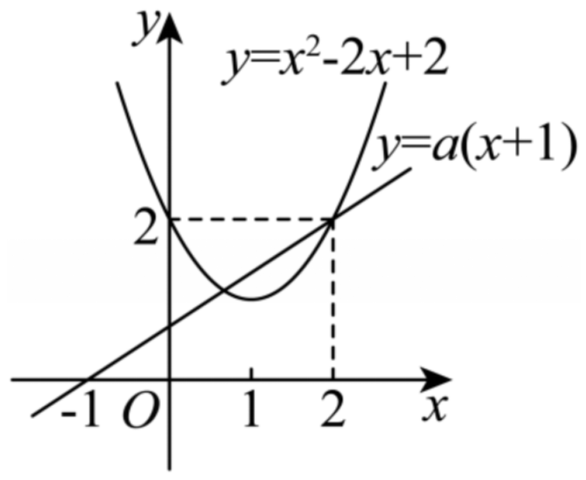
\includegraphics[width=0.30\textwidth]{figures/gao75_q12_graph.png}
\end{center}
% 原卷此处作“≥”，与题干严格不等号方向不一致，照录（见文件头“原卷笔误/存疑”①）
\step{由集合 $A$ 是“$2$ 集合”，故集合 $A$ 中只有一个元素，}
\step{得 $\begin{cases}2^2-2\times2+2\geqslant(2+1)a\\ 1^2-2\times1+2<(1+1)a\end{cases}$，解得 $\dfrac12<a\leqslant\dfrac23$，}
\step{故正实数 $a$ 的取值范围是 $\dfrac12<a\leqslant\dfrac23$.}
\solend
\fi

\end{enumerate}

\bigsec{二、选择题}

\begin{enumerate}
\setcounter{enumi}{12}

\item 已知全集 $U=\R$，集合 $A=\{x\mid x^2<4\}$，$B=\{y\mid y=x^2\}$，则图中阴影部分所表示的集合为\mbox{（\quad）}

\begin{center}
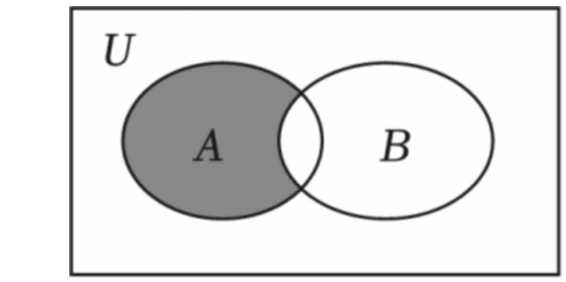
\includegraphics[width=0.26\textwidth]{figures/gao75_q13_venn.png}
\end{center}

\keepwithprev
A. $\{-2,-1,0\}$\qquad B. $(-\infty,4)$\qquad C. $(-2,0)$\qquad D. $(-2,0]$

\ifanswer
\solbegin
\step{集合 $A=\{x\mid x^2<4\}=(-2,2)$，$B=\{y\mid y=x^2\}=[0,+\infty)$，}
\step{图中阴影部分所表示的集合是 $A\cap\overline{B}=(-2,0)$. 故选 $C$.}
\solend
\fi

\item 已知 $x\in\R$，则“$\dfrac1x>1$”是“$x<1$”的\mbox{（\quad）}

\keepwithprev
A. 充分非必要条件\qquad B. 必要非充分条件\qquad C. 充要条件\qquad D. 既非充分又非必要条件

\ifanswer
\solbegin
\step{“$\dfrac1x>1$”$\Leftrightarrow0<x<1$，所以“$\dfrac1x>1$”是“$x<1$”的充分不必要条件. 故选 $A$.}
\solend
\fi

\item 已知集合 $M=\{x\mid x=m+\dfrac16,\,m\in\Z\}$，$N=\{x\mid x=\dfrac n2-\dfrac13,\,n\in\Z\}$，\\
$P=\{x\mid x=\dfrac p2+\dfrac16,\,p\in\Z\}$，则 $M$、$N$、$P$ 的关系为\mbox{（\quad）}

\keepwithprev
A. $M=N\subseteq P$\qquad B. $M\subseteq N=P$\qquad C. $M\subseteq N\subseteq P$\qquad D. $N\subseteq P\subseteq M$

\ifanswer
\solbegin
\step{集合 $N=\{x\mid x=\dfrac n2-\dfrac13,\,n\in\Z\}$，则 $x=\dfrac n2-\dfrac13=\dfrac{3n-2}6$，$n\in\Z$.}
\step{$P=\{x\mid x=\dfrac p2+\dfrac16,\,p\in\Z\}$，则 $x=\dfrac p2+\dfrac16=\dfrac{3p+1}6$，$p\in\Z$.}
\step{$M=\{x\mid x=m+\dfrac16,\,m\in\Z\}$，则 $x=m+\dfrac16=\dfrac{6m+1}6$，$m\in\Z$.}
\step{$M$、$N$、$P$ 三者分母相同，所以只需要比较他们的分子.}
\step{$M$：$6$ 的倍数$+1$，$N=P$：$3$ 的倍数$+1$，所以 $M\subseteq N=P$. 故选 $B$.}
\solend
\fi

\item 设集合 $P_1=\{x\mid x^2+ax+1>0\}$，$P_2=\{x\mid x^2+ax+2>0\}$，$Q_1=\{x\mid x^2+x+b>0\}$，$Q_2=\{x\mid x^2+2x+b>0\}$ 其中 $a,b\in\R$，给出下列两个命题：命题 $q_1$：对任意的 $a$，$P_1$ 是 $P_2$ 的子集；命题 $q_2$：对任意的 $b$，$Q_1$ 不是 $Q_2$ 的子集. 下列说法正确的是\mbox{（\quad）}

\keepwithprev
A. 命题 $q_1$ 是真命题，命题 $q_2$ 是假命题\qquad B. 命题 $q_1$ 是假命题，命题 $q_2$ 是真命题

C. 命题 $q_1$、$q_2$ 都是真命题\qquad D. 命题 $q_1$、$q_2$ 都是假命题

\ifanswer
\solbegin
\step{对于集合 $P_1=\{x\mid x^2+ax+1>0\}$，$P_2=\{x\mid x^2+ax+2>0\}$，}
\step{当 $m\in P_1$，即 $m^2+am+1>0$，得 $m^2+am+2>0$，}
\step{即有 $m\in P_2$，得对任意 $a$，$P_1$ 是 $P_2$ 的子集，命题 $q_1$ 为真命题；}
\step{当 $b=5$ 时，$Q_1=\{x\mid x^2+x+5>0\}=\R$，$Q_2=\{x\mid x^2+2x+5>0\}=\R$，}
\step{得 $Q_1$ 是 $Q_2$ 的子集；}
\step{存在 $b$，使得 $Q_1$ 是 $Q_2$ 的子集，故命题 $q_2$ 是假命题.}
\step{故选 $A$.}
\solend
\fi

\end{enumerate}

\bigsec{三、解答题}

\begin{enumerate}
\setcounter{enumi}{16}

\item 设集合 $A=\{x\mid x^2-2x=0\}$，$B=\{x\mid x^2+2(a+1)x+a^2-1=0\}$.

（1）写出集合 $A$ 的所有子集；

（2）若 $A\cap B=B$，求实数 $a$ 的取值范围.

\ifanswer
\solbegin
\stepm{(1)}{由 $x^2-2x=0$，得 $x=2$ 或 $x=0$，所以 $A=\{0,2\}$，}
\step{故集合 $A$ 的所有子集为 $\varnothing$、$\{0\}$、$\{2\}$、$\{0,2\}$.}
\stepm{(2)}{因为 $A\cap B=B$，所以 $B\subseteq A$，}
\step{方程 $x^2+2(a+1)x+a^2-1=0$，$\Delta=4(a+1)^2-4(a^2-1)=8a+8$，}
\step{若 $\Delta<0$，即 $a<-1$，方程 $x^2+2(a+1)x+a^2-1=0$ 无解，}
\step{此时 $B=\varnothing$，满足题意；}
\step{若 $\Delta=0$，即 $a=-1$，由 $x^2+2(a+1)x+a^2-1=0$，即 $x^2=0$，}
\step{解得 $x=0$，此时 $B=\{0\}$，满足题意；}
\step{若 $\Delta>0$，即 $a>-1$，要使 $B\subseteq A$，}
\step{则方程 $x^2+2(a+1)x+a^2-1=0$ 的解集为 $\{0,2\}$，}
\step{则 $\begin{cases}2+0=-2(a+1)\\ 2\times0=a^2-1\end{cases}$，$a$ 不存在.}
\step{综上所述，$a\leqslant-1$，即实数 $a$ 的取值范围为 $\{a\mid a\leqslant-1\}$.}
\solend
\fi

\ansspace

\item 已知全集 $U=\R$，集合 $A=\left\{x\,\middle|\,\dfrac{x-1}{x-3}<0\right\}$，$B=\{x\mid|x-a|<2\}$.

（1）当 $a=1$ 时，试用区间表示集合 $A$、$B$；

（2）若 $A\cup B=B$，求实数 $a$ 的取值范围.

\ifanswer
\solbegin
\stepm{(1)}{不等式 $\dfrac{x-1}{x-3}<0$ 可化为 $(x-1)(x-3)<0$，解得 $1<x<3$，即 $A=(1,3)$，}
\step{当 $a=1$ 时，$|x-1|<2$，则 $-2<x-1<2$，解得 $-1<x<3$，}
\step{即 $B=(-1,3)$；}
\stepm{(2)}{由不等式 $|x-a|<2$ 得 $-2<x-a<2$，解得 $-2+a<x<2+a$，}
\step{即 $B=\{x\mid-2+a<x<2+a\}$，}
\step{因为 $A\cup B=B$，所以 $A\subseteq B$，则 $\begin{cases}-2+a\leqslant1\\ 2+a\geqslant3\end{cases}$，解得 $1\leqslant a\leqslant3$，}
\step{即实数 $a$ 的取值范围为 $[1,3]$.}
\solend
\fi

\ansspace

\item 法国数学家弗朗索瓦·韦达 1615 年在著作《论方程的识别与订正》中建立了方程根与系数的关系. 发现一元二次方程 $ax^2+bx+c=0$，$a\neq0$ 的根与系数有如下的关系：

$x_1+x_2=-\dfrac ba$，$x_1x_2=\dfrac ca$，此即为韦达定理. 韦达定理的逆定理仍成立：如果两个数 $x_1$，$x_2$ 满足 $x_1+x_2=-\dfrac ba$，$x_1x_2=\dfrac ca$，则这两个数 $x_1$、$x_2$ 是方程 $ax^2+bx+c=0$，$a\neq0$ 的两个根. 例如：$m+n=-3$，$mn=2$，则 $m$、$n$ 是方程 $x^2+3x+2=0$ 的两个根. 请根据上述材料解决以下问题.

（1）已知 $m$、$n$ 是两个不相等的实数，满足 $m^2-6m-5=0$，$n^2-6n-5=0$，求 $\dfrac1m+\dfrac1n$ 的值；

（2）已知实数 $x$、$y$ 满足 $x+y+xy=17$，$x^2y+xy^2=72$，求 $x^2+y^2$ 的值.

\ifanswer
\solbegin
\stepm{(1)}{由题意，不相等的实数 $m$、$n$ 满足 $m^2-6m-5=0$、$n^2-6n-5=0$，}
\step{因此 $m$、$n$ 是一元二次方程 $x^2-6x-5=0$ 的两个不等实根.}
\step{由韦达定理得 $m+n=6$，$mn=-5$，因此 $\dfrac1m+\dfrac1n=\dfrac{m+n}{mn}=\dfrac6{-5}=-\dfrac65$.}
\stepm{(2)}{令 $s=x+y$，$t=xy$，}
\step{因为 $x+y+xy=17$，$x^2y+xy^2=72$，}
\step{即 $x+y+xy=17$，$xy(x+y)=72$，将已知条件变形得 $\begin{cases}s+t=17\\ st=72\end{cases}$.}
\step{由韦达定理逆定理，$s$、$t$ 是一元二次方程 $z^2-17z+72=0$ 的两个实根，}
\step{解方程得 $z_1=8$，$z_2=9$，即有两组解 $\begin{cases}s=8\\ t=9\end{cases}$ 和 $\begin{cases}s=9\\ t=8\end{cases}$.}
\step{当 $\begin{cases}s=8\\ t=9\end{cases}$ 时，$x$、$y$ 是方程 $w^2-8w+9=0$ 的根，}
\step{判别式 $\Delta=8^2-4\times1\times9=64-36=28>0$，符合题意，}
\step{此时 $x^2+y^2=(x+y)^2-2xy=s^2-2t=8^2-2\times9=64-18=46$；}
\step{当 $\begin{cases}s=9\\ t=8\end{cases}$ 时，$x$、$y$ 是方程 $w^2-9w+8=0$ 的根，}
\step{判别式 $\Delta=9^2-4\times1\times8=81-32=49>0$，符合题意，}
\step{此时 $x^2+y^2=(x+y)^2-2xy=s^2-2t=9^2-2\times8=81-16=65$.}
\step{综上，$x^2+y^2$ 的值为 $46$ 或 $65$.}
\solend
\fi

\ansspace

\item 已知关于 $x$ 的不等式 $ax^2-(a+1)x+b<0$.

（1）若不等式的解集是 $\{x\mid1<x<5\}$，求 $a+b$ 的值；

（2）若 $b=-\dfrac12$ 且不等式的解集为 $\R$，求 $a$ 取值范围；

（3）若 $b=1$，讨论此不等式的解集.

\ifanswer
\solbegin
\stepm{(1)}{由题意得 $1$ 和 $5$ 是方程 $ax^2-(a+1)x+b=0$ 的两个根且 $a>0$，}
\step{所以 $1+5=\dfrac{a+1}a$，$1\times5=\dfrac ba$，解得 $a=\dfrac15$，$b=1$，所以 $a+b=\dfrac65$.}
\stepm{(2)}{若 $b=-\dfrac12$，则不等式为 $ax^2-(a+1)x-\dfrac12<0$，}
\step{当 $a\neq0$，则有 $\begin{cases}a<0\\ \Delta=(a+1)^2+2a<0\end{cases}$，解得 $-2-\sqrt3<a<-2+\sqrt3$；}
\step{当 $a=0$，不等式即为 $-x-\dfrac12<0$，则 $x>-\dfrac12$，不合题意；}
\step{所以 $a$ 的取值范围是 $(-2-\sqrt3,-2+\sqrt3)$.}
\stepm{(3)}{若 $b=1$，则不等式为 $ax^2-(a+1)x+1<0$，即 $(ax-1)(x-1)<0$.}
\step{当 $a\neq0$ 时，由 $ax^2-(a+1)x+1<0$ 得 $(ax-1)(x-1)<0$.}
\step{方程 $(ax-1)(x-1)=0$ 的根为 $x=\dfrac1a$ 或 $x=1$，}
\step{当 $0<a<1$ 时，$\dfrac1a>1$，则不等式的解集为 $\left(1,\dfrac1a\right)$；}
\step{当 $a<0$ 时，$\dfrac1a<1$，则不等式的解集为 $\left(-\infty,\dfrac1a\right)\cup(1,+\infty)$；}
\step{当 $a=1$ 时，不等式即为 $(x-1)^2<0$，则不等式的解集为 $\varnothing$；}
\step{当 $a>1$ 时，$\dfrac1a<1$，则不等式的解集为 $\left(\dfrac1a,1\right)$；}
\step{当 $a=0$ 时，不等式为 $-x+1<0$，则不等式的解集为 $(1,+\infty)$；}
\step{综上所述，当 $a<0$ 时，不等式的解集为 $\left(-\infty,\dfrac1a\right)\cup(1,+\infty)$；}
\step{当 $a=0$ 时，不等式的解集为 $(1,+\infty)$；}
\step{当 $0<a<1$ 时，不等式的解集为 $\left(1,\dfrac1a\right)$；}
\step{当 $a=1$ 时，不等式的解集为 $\varnothing$；}
\step{当 $a>1$ 时，不等式的解集为 $\left(\dfrac1a,1\right)$.}
\solend
\fi

\ansspace

\item 已知关于 $x$ 的不等式① $x^2+2cx+c>0$，② $x^2+cx+c^2-1>0$，其中 $c$ 是实数.

（1）若 $1$ 是不等式②的一个解，求实数 $c$ 的取值范围；

（2）证明：不等式①、②中至多有一个恒成立；

（3）当 $c=0$ 时，“$x$ 满足 $|mx^2-4x+3|>5$”的一个必要非充分条件是“$x$ 满足 $x^2+cx+c^2-1>0$，求实数 $m$ 的取值范围.

\ifanswer
\solbegin
\stepm{(1)}{因为 $1$ 是不等式②的一个解，所以 $1+c+c^2-1>0$，}
\step{即 $c(c+1)>0$，解得 $c>0$ 或 $c<-1$，}
\step{所以实数 $c$ 的取值范围为 $(-\infty,-1)\cup(0,+\infty)$.}
\stepm{(2)}{假设不等式①、②都恒成立，}
\step{不等式① $x^2+2cx+c>0$ 恒成立，所以 $4c^2-4c<0$，所以 $0<c<1$；}
\step{② $x^2+cx+c^2-1>0$ 恒成立，所以 $c^2-4(c^2-1)<0$，$c^2>\dfrac43$，}
\step{解得 $c>\dfrac{2\sqrt3}3$ 或 $c<-\dfrac{2\sqrt3}3$；}
\step{所以当不等式①、②都恒成立时，}
\step{不等式组 $\begin{cases}0<c<1\\ c\in\left(-\infty,-\dfrac{2\sqrt3}3\right)\cup\left(\dfrac{2\sqrt3}3,+\infty\right)\end{cases}$ 无解，}
\step{所以假设不成立，}
\step{所以不等式①、②中至多有一个恒成立.}
\stepm{(3)}{当 $c=0$ 时，由 $x^2+cx+c^2-1>0$ 得 $x^2-1>0$，}
\step{解集为 $(-\infty,-1)\cup(1,+\infty)$.}
\step{记集合 $A=\{x\mid|mx^2-4x+3|>5\}$，集合 $B=\{x\mid x<-1\text{ 或 }x>1\}$.}
\step{由“$x$ 满足 $|mx^2-4x+3|>5$”的一个必要非充分条件是}
\step{“$x$ 满足 $x^2+cx+c^2-1>0$”得 $A$ 是 $B$ 的真子集.}
\step{所以 $\overline{B}$ 是 $A$ 的真子集，即对任意 $x\in[-1,1]$，$|mx^2-4x+3|\leqslant5$ 恒成立.}
\step{当 $x=0$ 时，不等式 $-5\leqslant mx^2-4x+3\leqslant5$ 恒成立；}
\step{当 $x\in[-1,0)\cup(0,1]$ 时，}
\step{则 $mx^2-4x+3\geqslant-5$ 与 $mx^2-4x+3\leqslant5$ 同时成立.}
\step{①由 $mx^2-4x+3\geqslant-5$，得 $m\geqslant\dfrac{4x-8}{x^2}$，求值域得 $\dfrac{4x-8}{x^2}$ 的最大值 $=-4$，}
\step{所以 $m\geqslant-4$.}
\step{②由 $mx^2-4x+3\leqslant5$，得 $m\leqslant\dfrac{4x+2}{x^2}$，求值域得 $\dfrac{4x+2}{x^2}$ 的最小值 $=-2$，}
\step{所以 $m\leqslant-2$.}
\step{综上所述，实数 $m$ 的取值范围为 $[-4,-2]$.}
\solend
\fi

\ansspace*[7]

\end{enumerate}

\end{document}
"
% 紧凑版：xelatex "\def\iscompact{1}% 高一75_市二中学_10月月考.tex
%   —— 高一上数学“2026-2027 年市二中学高一上 10 月月考”（讲评版）
% 试卷版：xelatex 高一75_市二中学_10月月考.tex
% 答案版：xelatex "\def\isanswer{1}\input{高一75_市二中学_10月月考.tex}"
% 紧凑版：xelatex "\def\iscompact{1}\input{高一75_市二中学_10月月考.tex}"
%
% 原始材料：微信公众号“魔都数学加油站”文章，连载“27学年高一75”；
% 原文标题“27学年高一75——2026-2027年上海市市二中学高一上10月月考”；
% 原文链接：https://mp.weixin.qq.com/s/dhxtwWEZgKLxeKdkbWqOhw。
% 页面标注发布时间 2026-10-22 21:45（上海）。
% 正文为 11 张 PNG 页（`原图/高一75_市二中学_10月月考/01..11.png`）：
% 第 2、4、5、6、9 页为 4762×6735，其余 6 页为 2560×3620，均按页序读取。
% 11 页全为试卷正文页（卷首标题在第 1 页页顶，卷末第 21 题 (3) 解析止于第 11 页），
% 无封面页、目录页、二维码或宣传页。粉色斜排“魔都数学加油站”为卷面水印，未录入。
%
% 卷首标题：照卷面印作“2026-2027 年市二中学高一上 10 月月考”（黑体加粗一行）。
% 原卷年份区间用半角连字符，本稿按全稿惯例排 en dash；原卷无副标题。
%
% 篇幅与题号：原卷自第 3 题起编号（第 1、2 题不在本卷内）。填空题 3—12（10 题）、
% 选择题 13—16（4 题）、解答题 17—21（5 题），共 19 题。本稿沿用原节与原题号，
% 只改排为全稿统一的大节样式。
%
% 讲评版：原卷第 4 题只印【答案】（“$[-1,2]$”），本稿只给 \ans{}；其余 18 题均印
% 【解析】，用 \solbegin…\solend。四道选择题的作答括号原卷即留空，答案写在解析末句
% “故选 C／A／B／A”，照录在解析内，不另提 \ans{}。
%
% 副标题：原卷未印副标题。本稿按“知识模块”口径标作“集合与常用逻辑用语、不等式”：
% 19 题中集合与常用逻辑用语 9 题（第 3、4、5、8、10、12、13、15、17、18 题中的集合题），
% 不等式 10 题（第 6、7、9、11、19、20、21 题及第 12、20 题的不等式部分），两类均确有
% 分量，故并标。口径同 高一63、高一68—74。
%
% 与原卷的排版差异：
%   ① 原卷每题下直接印【答案】/【解析】，本稿按全稿惯例将答案与解析置于答案版；
%   ② 原卷未印副标题，本稿按“知识模块”口径补出；
%   ③ 原卷填空横线约四个字宽，本稿按全稿惯例统一排 \blankline[4.4em]；
%   ④ 原卷数集记号排粗体 $\mathbf{R}$（第 5、6、7、9、10、14、18、20、21 题），本稿
%      按全稿惯例改用 $\R$（同 高一68—74）；第 11 题的“解集为 $\R$”同此；
%   ⑤ 原卷句末标点多为西文句点，均逐处照录；
%   ⑥ 第 17—21 题的子问原卷印作“（1）…（2）…”，本稿按 高一69—74 成例用行内
%      “（1）（2）（3）”段，解析中的子问标号用 \stepm{(1)}{…}；
%   ⑦ 每道解答题原卷未留作答空白，本稿按全稿惯例加 \ansspace（末题用 \ansspace*）；
%   ⑧ 选择题的作答括号原卷排半角“(    )”，本稿按全稿惯例排 \mbox{（\quad）}；
%      选项行排照原卷——第 13、14 题一行四条，第 15、16 题一行四条；
%   ⑨ 第 9、12、15、17—21 题解析中的不等式组／方程组，原卷均排作“{”连接的多行式，
%      本稿按全稿惯例排 cases；
%   ⑩ 第 12 题解析有一幅“抛物线 + 直线”图：原卷印在解析第 3 行右侧、题干无“如图”二字
%      （解析里写“两函数图象如图：”）。本稿按原卷截图裁取（`figures/gao75_q12_graph.png`，
%      由第 3 页原图裁出、去除粉色水印后转灰度，未放大），放在答案版解析第 3 条之后；
%   ⑪ 第 13 题题干中间有一幅韦恩图（全集矩形内含 A、B 两圆，A 涂灰）：原卷印在题干
%      右侧、题干句子被图隔开。本稿按原卷截图裁取（`figures/gao75_q13_venn.png`，由第 3
%      页原图裁出、去除粉色水印后转灰度，并抹去左侧侵入的“分”字），放在题干之后、
%      选项之前，仅答案版出。
%
% 原卷笔误/存疑（均照录未改，正文对应处另有 % 注）：
%   ① 第 12 题解析列不等式组时写 $2^2-2\times2+2\geqslant(2+1)a$，与
%      $x^2-2x+2<a(x+1)$ 的严格不等号方向不一致；原卷如此，照录未改。
%   ② 第 14 题选项 A—D 的“充分非必要”“必要非充分”“既非充分又非必要”与原卷
%      其它题的“充分不必要”写法不同，照录未统一。
%   ④ 第 21 题 (3) 题干的“$x$ 满足 $|mx^2-4x+3|>5$”的一个必要非充分条件是
%      “$x$ 满足 $x^2+cx+c^2-1>0$，原卷只有左引号、无右引号（且逗号在引号内），
%      本稿照录未补。
%   ③ 第 20 题 (2) 的解集写成 $(-2-\sqrt3,-2+\sqrt3)$，其中 $a<0$ 与 $\Delta<0$ 联立后
%      左端点应为 $-2-\sqrt3$、右端点为 $-2+\sqrt3$；原卷如此，照录未改。
%
% 行数核对：逐题数 \step/\stepm 条数与原卷【解析】印刷行数，18 题逐一相符，
% 合计 132 条 / 132 行（Q3：6；Q5：1；Q6：2；Q7：1；Q8：2；Q9：3；Q10：10；
% Q11：8；Q12：6；Q13：2；Q14：1；Q15：5；Q16：7；Q17：12；Q18：7；Q19：15；
% Q20：19；Q21：25）。另第 4 题只印【答案】，提 \ans{}，不计入 \step 账。
%
% 插图：第 12 题解析的抛物线图、第 13 题题干的韦恩图，见上⑩⑪；其余题干无配图。
%
\documentclass[a4paper,11pt]{article}
\usepackage{common}

\begin{document}

\examtitlest[3]{2026--2027 年市二中学高一上 10 月月考}{集合与常用逻辑用语、不等式}

\bigsec{一、填空题}

\begin{enumerate}
\setcounter{enumi}{2}

\item 已知集合 $A=\{a,a^2\}$，且 $1\in A$，则 $a=$\blankline[4.4em].

\ifanswer
\solbegin
\step{因为 $1\in A=\{a,a^2\}$，所以 $a=1$ 或 $a^2=1$.}
\step{又集合 $A=\{a,a^2\}$ 是用列举法写出两个元素的，其元素必须互异，故 $a\neq a^2$，}
\step{即 $a\neq0$ 且 $a\neq1$，所以 $a=1$ 应舍去；}
\step{由 $a^2=1$ 得 $a=1$（舍去）或 $a=-1$.}
\step{当 $a=-1$ 时，$A=\{-1,1\}$，满足 $1\in A$ 且两个元素互异.}
\step{故 $a=-1$.}
\solend
\fi

\item 已知集合 $A=[-1,1]$，$B=[0,2]$，则 $A\cup B=$\blankline[4.4em].

\ifanswer
\ans{$[-1,2]$}
\fi

\item 已知全集 $U=\R$，集合 $A=\{x\mid x\neq1\}$，则 $\overline{A}=$\blankline[4.4em].

\ifanswer
\solbegin
\step{因为全集 $U=\R$，集合 $A=\{x\mid x\neq1\}$，所以 $\overline{A}=\{x\mid x=1\}$.}
\solend
\fi

\item 设 $x\in\R$，不等式 $x^2-4x<0$ 的解集用区间表示是\blankline[4.4em].

\ifanswer
\solbegin
\step{因为 $x^2-4x<0$，即 $x(x-4)<0$，所以 $0<x<4$，}
\step{所以 $x(x-4)<0$ 的解集为 $(0,4)$.}
\solend
\fi

\item 已知 $m\in\R$，若关于 $x$ 的方程 $2mx^2+3x+m-1=m^2\cdot x^2+(m+1)x+1$ 解集为 $\R$，则 $m$ 的值为\blankline[4.4em].

\ifanswer
\solbegin
\step{由题意得 $2m=m^2$，$3=m+1$，$m-1=1$，所以 $m=2$.}
\solend
\fi

\item 设 $\alpha:x\leqslant m$，$\beta:|x-2|\leqslant1$，若 $\alpha$ 是 $\beta$ 的必要条件，则实数 $m$ 的取值范围是\blankline[4.4em].

\ifanswer
\solbegin
\step{由 $|x-2|\leqslant1$，得 $-1\leqslant x-2\leqslant1$，解得 $1\leqslant x\leqslant3$，}
\step{因为 $\alpha$ 是 $\beta$ 的必要条件，所以 $\{x\mid1\leqslant x\leqslant3\}\subseteq\{x\mid x\leqslant m\}$，得 $m\geqslant3$.}
\solend
\fi

\item 设 $a\in\R$，若关于 $x$ 的不等式 $\dfrac{a}{x-1}\leqslant1$ 的解集是 $(-\infty,1)\cup[2,+\infty)$，则 $a$ 的值为\blankline[4.4em].

\ifanswer
\solbegin
\step{不等式可变形为 $\dfrac{a+1-x}{x-1}\leqslant0$，等价于 $\begin{cases}(a+1-x)(x-1)\leqslant0\\ x-1\neq0\end{cases}$，}
\step{因为原不等式的解集是 $(-\infty,1)\cup[2,+\infty)$，}
\step{所以 $1$，$2$ 是方程 $(a+1-x)(x-1)=0$ 的两根，所以 $a+1=2$，解得 $a=1$.}
\solend
\fi

\item 下列命题：① “$x>1$ 或 $y>1$”的否定形式是“$x\leqslant1$ 或 $y\leqslant1$”，② 若 $A\cup B=B$，则 $A\subseteq B$，③ 方程 $ax+1=0$ 的解是 $x=-\frac1a$，④ “$ac=bc$”是“$a=b$”的必要非充分条件，⑤ “任意 $x\in\R$，$f(x)=f(-x)$”的否定形式是“存在 $x_0\in\R$，使得 $f(x_0)\neq f(-x_0)$”其中真命题的序号是\blankline[4.4em]（填写序号）.

\ifanswer
\solbegin
\step{①假命题：“$x>1$ 或 $y>1$”的否定形式是“$x\leqslant1$ 且 $y\leqslant1$”；}
\step{②真命题：$A\cup B=B\Leftrightarrow A\subseteq B$；}
\step{③假命题：当 $a=0$ 时，方程无解，因此该命题忽略了 $a=0$ 的情况；}
\step{④真命题：先判断必要性：若 $a=b$，则有 $ac=bc$，所以必要性成立；}
\step{再判断充分性：若 $ac=bc$，即 $(a-b)c=0$，当 $c=0$ 时，$a$ 和 $b$ 可以不相等，}
\step{因此充分性不成立.}
\step{⑤真命题：全称命题的否定是存在量词命题，}
\step{“任意 $x\in\R$，$f(x)=f(-x)$”的否定形式是}
\step{“存在 $x_0\in\R$，使得 $f(x_0)\neq f(-x_0)$”，表述正确.}
\step{故正确的是②④⑤.}
\solend
\fi

\item 为了加强家校联系，蔡老师组建了一个由学生、家长和教师组成的微信群. 已知该群中男学生人数多于女学生人数，女学生人数多于家长人数，家长人数多于教师人数，教师人数的两倍多于男学生人数. 则该微信群人数的最小值为\blankline[4.4em].

\ifanswer
\solbegin
\step{设男学生、女学生、家长、教师的人数分别为 $M$、$F$、$P$、$T$，}
\step{它们都是正整数.}
\step{由题意得 $M>F>P>T$，且教师人数的两倍多于男学生人数，即 $2T>M$.}
\step{由 $M>F>P>T$ 得 $M\geqslant T+3$；}
\step{又 $2T>M\geqslant T+3$，所以 $2T>T+3$，解得 $T>3$，故教师人数最少为 $T=4$.}
\step{当 $T=4$ 时，为使总人数最少，取 $P=5$、$F=6$、$M=7$，}
\step{此时 $7>6>5>4$ 且 $2\times4=8>7$，满足题意.}
\step{于是微信群人数为 $4+5+6+7=22$，所以该微信群人数的最小值为 $22$.}
\solend
\fi

\item 若集合 $M$ 有 $k$ 个子集，则称集合 $M$ 为“$k$ 集合”，\\
已知集合 $A=\{x\mid x^2-(a+2)x+2-a<0,\,x\in\Z\}$ 是“$2$ 集合”，则正实数 $a$ 的取值范围是\blankline[4.4em].

\ifanswer
\solbegin
\step{由 $x^2-(a+2)x+2-a<0$，得 $x^2-2x+2<a(x+1)$，}
\step{设二次函数 $y=x^2-2x+2$ 与一次函数 $y=a(x+1)$，}
\needvspace{13\baselineskip}
\step{由 $a>0$，$y=a(x+1)$ 过定点 $(-1,0)$，两函数图象如图：}
\begin{center}
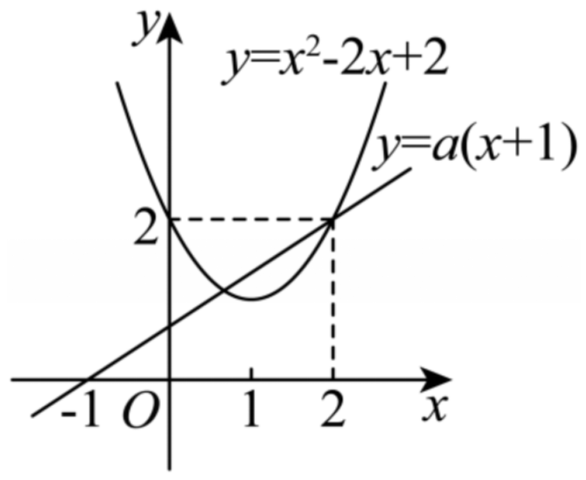
\includegraphics[width=0.30\textwidth]{figures/gao75_q12_graph.png}
\end{center}
% 原卷此处作“≥”，与题干严格不等号方向不一致，照录（见文件头“原卷笔误/存疑”①）
\step{由集合 $A$ 是“$2$ 集合”，故集合 $A$ 中只有一个元素，}
\step{得 $\begin{cases}2^2-2\times2+2\geqslant(2+1)a\\ 1^2-2\times1+2<(1+1)a\end{cases}$，解得 $\dfrac12<a\leqslant\dfrac23$，}
\step{故正实数 $a$ 的取值范围是 $\dfrac12<a\leqslant\dfrac23$.}
\solend
\fi

\end{enumerate}

\bigsec{二、选择题}

\begin{enumerate}
\setcounter{enumi}{12}

\item 已知全集 $U=\R$，集合 $A=\{x\mid x^2<4\}$，$B=\{y\mid y=x^2\}$，则图中阴影部分所表示的集合为\mbox{（\quad）}

\begin{center}
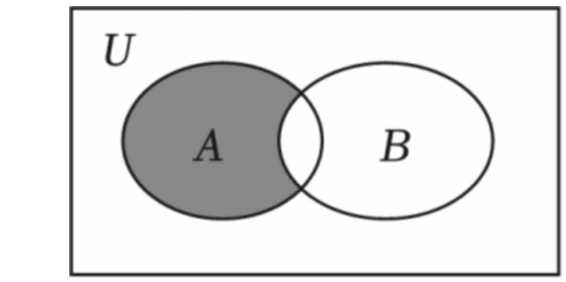
\includegraphics[width=0.26\textwidth]{figures/gao75_q13_venn.png}
\end{center}

\keepwithprev
A. $\{-2,-1,0\}$\qquad B. $(-\infty,4)$\qquad C. $(-2,0)$\qquad D. $(-2,0]$

\ifanswer
\solbegin
\step{集合 $A=\{x\mid x^2<4\}=(-2,2)$，$B=\{y\mid y=x^2\}=[0,+\infty)$，}
\step{图中阴影部分所表示的集合是 $A\cap\overline{B}=(-2,0)$. 故选 $C$.}
\solend
\fi

\item 已知 $x\in\R$，则“$\dfrac1x>1$”是“$x<1$”的\mbox{（\quad）}

\keepwithprev
A. 充分非必要条件\qquad B. 必要非充分条件\qquad C. 充要条件\qquad D. 既非充分又非必要条件

\ifanswer
\solbegin
\step{“$\dfrac1x>1$”$\Leftrightarrow0<x<1$，所以“$\dfrac1x>1$”是“$x<1$”的充分不必要条件. 故选 $A$.}
\solend
\fi

\item 已知集合 $M=\{x\mid x=m+\dfrac16,\,m\in\Z\}$，$N=\{x\mid x=\dfrac n2-\dfrac13,\,n\in\Z\}$，\\
$P=\{x\mid x=\dfrac p2+\dfrac16,\,p\in\Z\}$，则 $M$、$N$、$P$ 的关系为\mbox{（\quad）}

\keepwithprev
A. $M=N\subseteq P$\qquad B. $M\subseteq N=P$\qquad C. $M\subseteq N\subseteq P$\qquad D. $N\subseteq P\subseteq M$

\ifanswer
\solbegin
\step{集合 $N=\{x\mid x=\dfrac n2-\dfrac13,\,n\in\Z\}$，则 $x=\dfrac n2-\dfrac13=\dfrac{3n-2}6$，$n\in\Z$.}
\step{$P=\{x\mid x=\dfrac p2+\dfrac16,\,p\in\Z\}$，则 $x=\dfrac p2+\dfrac16=\dfrac{3p+1}6$，$p\in\Z$.}
\step{$M=\{x\mid x=m+\dfrac16,\,m\in\Z\}$，则 $x=m+\dfrac16=\dfrac{6m+1}6$，$m\in\Z$.}
\step{$M$、$N$、$P$ 三者分母相同，所以只需要比较他们的分子.}
\step{$M$：$6$ 的倍数$+1$，$N=P$：$3$ 的倍数$+1$，所以 $M\subseteq N=P$. 故选 $B$.}
\solend
\fi

\item 设集合 $P_1=\{x\mid x^2+ax+1>0\}$，$P_2=\{x\mid x^2+ax+2>0\}$，$Q_1=\{x\mid x^2+x+b>0\}$，$Q_2=\{x\mid x^2+2x+b>0\}$ 其中 $a,b\in\R$，给出下列两个命题：命题 $q_1$：对任意的 $a$，$P_1$ 是 $P_2$ 的子集；命题 $q_2$：对任意的 $b$，$Q_1$ 不是 $Q_2$ 的子集. 下列说法正确的是\mbox{（\quad）}

\keepwithprev
A. 命题 $q_1$ 是真命题，命题 $q_2$ 是假命题\qquad B. 命题 $q_1$ 是假命题，命题 $q_2$ 是真命题

C. 命题 $q_1$、$q_2$ 都是真命题\qquad D. 命题 $q_1$、$q_2$ 都是假命题

\ifanswer
\solbegin
\step{对于集合 $P_1=\{x\mid x^2+ax+1>0\}$，$P_2=\{x\mid x^2+ax+2>0\}$，}
\step{当 $m\in P_1$，即 $m^2+am+1>0$，得 $m^2+am+2>0$，}
\step{即有 $m\in P_2$，得对任意 $a$，$P_1$ 是 $P_2$ 的子集，命题 $q_1$ 为真命题；}
\step{当 $b=5$ 时，$Q_1=\{x\mid x^2+x+5>0\}=\R$，$Q_2=\{x\mid x^2+2x+5>0\}=\R$，}
\step{得 $Q_1$ 是 $Q_2$ 的子集；}
\step{存在 $b$，使得 $Q_1$ 是 $Q_2$ 的子集，故命题 $q_2$ 是假命题.}
\step{故选 $A$.}
\solend
\fi

\end{enumerate}

\bigsec{三、解答题}

\begin{enumerate}
\setcounter{enumi}{16}

\item 设集合 $A=\{x\mid x^2-2x=0\}$，$B=\{x\mid x^2+2(a+1)x+a^2-1=0\}$.

（1）写出集合 $A$ 的所有子集；

（2）若 $A\cap B=B$，求实数 $a$ 的取值范围.

\ifanswer
\solbegin
\stepm{(1)}{由 $x^2-2x=0$，得 $x=2$ 或 $x=0$，所以 $A=\{0,2\}$，}
\step{故集合 $A$ 的所有子集为 $\varnothing$、$\{0\}$、$\{2\}$、$\{0,2\}$.}
\stepm{(2)}{因为 $A\cap B=B$，所以 $B\subseteq A$，}
\step{方程 $x^2+2(a+1)x+a^2-1=0$，$\Delta=4(a+1)^2-4(a^2-1)=8a+8$，}
\step{若 $\Delta<0$，即 $a<-1$，方程 $x^2+2(a+1)x+a^2-1=0$ 无解，}
\step{此时 $B=\varnothing$，满足题意；}
\step{若 $\Delta=0$，即 $a=-1$，由 $x^2+2(a+1)x+a^2-1=0$，即 $x^2=0$，}
\step{解得 $x=0$，此时 $B=\{0\}$，满足题意；}
\step{若 $\Delta>0$，即 $a>-1$，要使 $B\subseteq A$，}
\step{则方程 $x^2+2(a+1)x+a^2-1=0$ 的解集为 $\{0,2\}$，}
\step{则 $\begin{cases}2+0=-2(a+1)\\ 2\times0=a^2-1\end{cases}$，$a$ 不存在.}
\step{综上所述，$a\leqslant-1$，即实数 $a$ 的取值范围为 $\{a\mid a\leqslant-1\}$.}
\solend
\fi

\ansspace

\item 已知全集 $U=\R$，集合 $A=\left\{x\,\middle|\,\dfrac{x-1}{x-3}<0\right\}$，$B=\{x\mid|x-a|<2\}$.

（1）当 $a=1$ 时，试用区间表示集合 $A$、$B$；

（2）若 $A\cup B=B$，求实数 $a$ 的取值范围.

\ifanswer
\solbegin
\stepm{(1)}{不等式 $\dfrac{x-1}{x-3}<0$ 可化为 $(x-1)(x-3)<0$，解得 $1<x<3$，即 $A=(1,3)$，}
\step{当 $a=1$ 时，$|x-1|<2$，则 $-2<x-1<2$，解得 $-1<x<3$，}
\step{即 $B=(-1,3)$；}
\stepm{(2)}{由不等式 $|x-a|<2$ 得 $-2<x-a<2$，解得 $-2+a<x<2+a$，}
\step{即 $B=\{x\mid-2+a<x<2+a\}$，}
\step{因为 $A\cup B=B$，所以 $A\subseteq B$，则 $\begin{cases}-2+a\leqslant1\\ 2+a\geqslant3\end{cases}$，解得 $1\leqslant a\leqslant3$，}
\step{即实数 $a$ 的取值范围为 $[1,3]$.}
\solend
\fi

\ansspace

\item 法国数学家弗朗索瓦·韦达 1615 年在著作《论方程的识别与订正》中建立了方程根与系数的关系. 发现一元二次方程 $ax^2+bx+c=0$，$a\neq0$ 的根与系数有如下的关系：

$x_1+x_2=-\dfrac ba$，$x_1x_2=\dfrac ca$，此即为韦达定理. 韦达定理的逆定理仍成立：如果两个数 $x_1$，$x_2$ 满足 $x_1+x_2=-\dfrac ba$，$x_1x_2=\dfrac ca$，则这两个数 $x_1$、$x_2$ 是方程 $ax^2+bx+c=0$，$a\neq0$ 的两个根. 例如：$m+n=-3$，$mn=2$，则 $m$、$n$ 是方程 $x^2+3x+2=0$ 的两个根. 请根据上述材料解决以下问题.

（1）已知 $m$、$n$ 是两个不相等的实数，满足 $m^2-6m-5=0$，$n^2-6n-5=0$，求 $\dfrac1m+\dfrac1n$ 的值；

（2）已知实数 $x$、$y$ 满足 $x+y+xy=17$，$x^2y+xy^2=72$，求 $x^2+y^2$ 的值.

\ifanswer
\solbegin
\stepm{(1)}{由题意，不相等的实数 $m$、$n$ 满足 $m^2-6m-5=0$、$n^2-6n-5=0$，}
\step{因此 $m$、$n$ 是一元二次方程 $x^2-6x-5=0$ 的两个不等实根.}
\step{由韦达定理得 $m+n=6$，$mn=-5$，因此 $\dfrac1m+\dfrac1n=\dfrac{m+n}{mn}=\dfrac6{-5}=-\dfrac65$.}
\stepm{(2)}{令 $s=x+y$，$t=xy$，}
\step{因为 $x+y+xy=17$，$x^2y+xy^2=72$，}
\step{即 $x+y+xy=17$，$xy(x+y)=72$，将已知条件变形得 $\begin{cases}s+t=17\\ st=72\end{cases}$.}
\step{由韦达定理逆定理，$s$、$t$ 是一元二次方程 $z^2-17z+72=0$ 的两个实根，}
\step{解方程得 $z_1=8$，$z_2=9$，即有两组解 $\begin{cases}s=8\\ t=9\end{cases}$ 和 $\begin{cases}s=9\\ t=8\end{cases}$.}
\step{当 $\begin{cases}s=8\\ t=9\end{cases}$ 时，$x$、$y$ 是方程 $w^2-8w+9=0$ 的根，}
\step{判别式 $\Delta=8^2-4\times1\times9=64-36=28>0$，符合题意，}
\step{此时 $x^2+y^2=(x+y)^2-2xy=s^2-2t=8^2-2\times9=64-18=46$；}
\step{当 $\begin{cases}s=9\\ t=8\end{cases}$ 时，$x$、$y$ 是方程 $w^2-9w+8=0$ 的根，}
\step{判别式 $\Delta=9^2-4\times1\times8=81-32=49>0$，符合题意，}
\step{此时 $x^2+y^2=(x+y)^2-2xy=s^2-2t=9^2-2\times8=81-16=65$.}
\step{综上，$x^2+y^2$ 的值为 $46$ 或 $65$.}
\solend
\fi

\ansspace

\item 已知关于 $x$ 的不等式 $ax^2-(a+1)x+b<0$.

（1）若不等式的解集是 $\{x\mid1<x<5\}$，求 $a+b$ 的值；

（2）若 $b=-\dfrac12$ 且不等式的解集为 $\R$，求 $a$ 取值范围；

（3）若 $b=1$，讨论此不等式的解集.

\ifanswer
\solbegin
\stepm{(1)}{由题意得 $1$ 和 $5$ 是方程 $ax^2-(a+1)x+b=0$ 的两个根且 $a>0$，}
\step{所以 $1+5=\dfrac{a+1}a$，$1\times5=\dfrac ba$，解得 $a=\dfrac15$，$b=1$，所以 $a+b=\dfrac65$.}
\stepm{(2)}{若 $b=-\dfrac12$，则不等式为 $ax^2-(a+1)x-\dfrac12<0$，}
\step{当 $a\neq0$，则有 $\begin{cases}a<0\\ \Delta=(a+1)^2+2a<0\end{cases}$，解得 $-2-\sqrt3<a<-2+\sqrt3$；}
\step{当 $a=0$，不等式即为 $-x-\dfrac12<0$，则 $x>-\dfrac12$，不合题意；}
\step{所以 $a$ 的取值范围是 $(-2-\sqrt3,-2+\sqrt3)$.}
\stepm{(3)}{若 $b=1$，则不等式为 $ax^2-(a+1)x+1<0$，即 $(ax-1)(x-1)<0$.}
\step{当 $a\neq0$ 时，由 $ax^2-(a+1)x+1<0$ 得 $(ax-1)(x-1)<0$.}
\step{方程 $(ax-1)(x-1)=0$ 的根为 $x=\dfrac1a$ 或 $x=1$，}
\step{当 $0<a<1$ 时，$\dfrac1a>1$，则不等式的解集为 $\left(1,\dfrac1a\right)$；}
\step{当 $a<0$ 时，$\dfrac1a<1$，则不等式的解集为 $\left(-\infty,\dfrac1a\right)\cup(1,+\infty)$；}
\step{当 $a=1$ 时，不等式即为 $(x-1)^2<0$，则不等式的解集为 $\varnothing$；}
\step{当 $a>1$ 时，$\dfrac1a<1$，则不等式的解集为 $\left(\dfrac1a,1\right)$；}
\step{当 $a=0$ 时，不等式为 $-x+1<0$，则不等式的解集为 $(1,+\infty)$；}
\step{综上所述，当 $a<0$ 时，不等式的解集为 $\left(-\infty,\dfrac1a\right)\cup(1,+\infty)$；}
\step{当 $a=0$ 时，不等式的解集为 $(1,+\infty)$；}
\step{当 $0<a<1$ 时，不等式的解集为 $\left(1,\dfrac1a\right)$；}
\step{当 $a=1$ 时，不等式的解集为 $\varnothing$；}
\step{当 $a>1$ 时，不等式的解集为 $\left(\dfrac1a,1\right)$.}
\solend
\fi

\ansspace

\item 已知关于 $x$ 的不等式① $x^2+2cx+c>0$，② $x^2+cx+c^2-1>0$，其中 $c$ 是实数.

（1）若 $1$ 是不等式②的一个解，求实数 $c$ 的取值范围；

（2）证明：不等式①、②中至多有一个恒成立；

（3）当 $c=0$ 时，“$x$ 满足 $|mx^2-4x+3|>5$”的一个必要非充分条件是“$x$ 满足 $x^2+cx+c^2-1>0$，求实数 $m$ 的取值范围.

\ifanswer
\solbegin
\stepm{(1)}{因为 $1$ 是不等式②的一个解，所以 $1+c+c^2-1>0$，}
\step{即 $c(c+1)>0$，解得 $c>0$ 或 $c<-1$，}
\step{所以实数 $c$ 的取值范围为 $(-\infty,-1)\cup(0,+\infty)$.}
\stepm{(2)}{假设不等式①、②都恒成立，}
\step{不等式① $x^2+2cx+c>0$ 恒成立，所以 $4c^2-4c<0$，所以 $0<c<1$；}
\step{② $x^2+cx+c^2-1>0$ 恒成立，所以 $c^2-4(c^2-1)<0$，$c^2>\dfrac43$，}
\step{解得 $c>\dfrac{2\sqrt3}3$ 或 $c<-\dfrac{2\sqrt3}3$；}
\step{所以当不等式①、②都恒成立时，}
\step{不等式组 $\begin{cases}0<c<1\\ c\in\left(-\infty,-\dfrac{2\sqrt3}3\right)\cup\left(\dfrac{2\sqrt3}3,+\infty\right)\end{cases}$ 无解，}
\step{所以假设不成立，}
\step{所以不等式①、②中至多有一个恒成立.}
\stepm{(3)}{当 $c=0$ 时，由 $x^2+cx+c^2-1>0$ 得 $x^2-1>0$，}
\step{解集为 $(-\infty,-1)\cup(1,+\infty)$.}
\step{记集合 $A=\{x\mid|mx^2-4x+3|>5\}$，集合 $B=\{x\mid x<-1\text{ 或 }x>1\}$.}
\step{由“$x$ 满足 $|mx^2-4x+3|>5$”的一个必要非充分条件是}
\step{“$x$ 满足 $x^2+cx+c^2-1>0$”得 $A$ 是 $B$ 的真子集.}
\step{所以 $\overline{B}$ 是 $A$ 的真子集，即对任意 $x\in[-1,1]$，$|mx^2-4x+3|\leqslant5$ 恒成立.}
\step{当 $x=0$ 时，不等式 $-5\leqslant mx^2-4x+3\leqslant5$ 恒成立；}
\step{当 $x\in[-1,0)\cup(0,1]$ 时，}
\step{则 $mx^2-4x+3\geqslant-5$ 与 $mx^2-4x+3\leqslant5$ 同时成立.}
\step{①由 $mx^2-4x+3\geqslant-5$，得 $m\geqslant\dfrac{4x-8}{x^2}$，求值域得 $\dfrac{4x-8}{x^2}$ 的最大值 $=-4$，}
\step{所以 $m\geqslant-4$.}
\step{②由 $mx^2-4x+3\leqslant5$，得 $m\leqslant\dfrac{4x+2}{x^2}$，求值域得 $\dfrac{4x+2}{x^2}$ 的最小值 $=-2$，}
\step{所以 $m\leqslant-2$.}
\step{综上所述，实数 $m$ 的取值范围为 $[-4,-2]$.}
\solend
\fi

\ansspace*[7]

\end{enumerate}

\end{document}
"
%
% 原始材料：微信公众号“魔都数学加油站”文章，连载“27学年高一75”；
% 原文标题“27学年高一75——2026-2027年上海市市二中学高一上10月月考”；
% 原文链接：https://mp.weixin.qq.com/s/dhxtwWEZgKLxeKdkbWqOhw。
% 页面标注发布时间 2026-10-22 21:45（上海）。
% 正文为 11 张 PNG 页（`原图/高一75_市二中学_10月月考/01..11.png`）：
% 第 2、4、5、6、9 页为 4762×6735，其余 6 页为 2560×3620，均按页序读取。
% 11 页全为试卷正文页（卷首标题在第 1 页页顶，卷末第 21 题 (3) 解析止于第 11 页），
% 无封面页、目录页、二维码或宣传页。粉色斜排“魔都数学加油站”为卷面水印，未录入。
%
% 卷首标题：照卷面印作“2026-2027 年市二中学高一上 10 月月考”（黑体加粗一行）。
% 原卷年份区间用半角连字符，本稿按全稿惯例排 en dash；原卷无副标题。
%
% 篇幅与题号：原卷自第 3 题起编号（第 1、2 题不在本卷内）。填空题 3—12（10 题）、
% 选择题 13—16（4 题）、解答题 17—21（5 题），共 19 题。本稿沿用原节与原题号，
% 只改排为全稿统一的大节样式。
%
% 讲评版：原卷第 4 题只印【答案】（“$[-1,2]$”），本稿只给 \ans{}；其余 18 题均印
% 【解析】，用 \solbegin…\solend。四道选择题的作答括号原卷即留空，答案写在解析末句
% “故选 C／A／B／A”，照录在解析内，不另提 \ans{}。
%
% 副标题：原卷未印副标题。本稿按“知识模块”口径标作“集合与常用逻辑用语、不等式”：
% 19 题中集合与常用逻辑用语 9 题（第 3、4、5、8、10、12、13、15、17、18 题中的集合题），
% 不等式 10 题（第 6、7、9、11、19、20、21 题及第 12、20 题的不等式部分），两类均确有
% 分量，故并标。口径同 高一63、高一68—74。
%
% 与原卷的排版差异：
%   ① 原卷每题下直接印【答案】/【解析】，本稿按全稿惯例将答案与解析置于答案版；
%   ② 原卷未印副标题，本稿按“知识模块”口径补出；
%   ③ 原卷填空横线约四个字宽，本稿按全稿惯例统一排 \blankline[4.4em]；
%   ④ 原卷数集记号排粗体 $\mathbf{R}$（第 5、6、7、9、10、14、18、20、21 题），本稿
%      按全稿惯例改用 $\R$（同 高一68—74）；第 11 题的“解集为 $\R$”同此；
%   ⑤ 原卷句末标点多为西文句点，均逐处照录；
%   ⑥ 第 17—21 题的子问原卷印作“（1）…（2）…”，本稿按 高一69—74 成例用行内
%      “（1）（2）（3）”段，解析中的子问标号用 \stepm{(1)}{…}；
%   ⑦ 每道解答题原卷未留作答空白，本稿按全稿惯例加 \ansspace（末题用 \ansspace*）；
%   ⑧ 选择题的作答括号原卷排半角“(    )”，本稿按全稿惯例排 \mbox{（\quad）}；
%      选项行排照原卷——第 13、14 题一行四条，第 15、16 题一行四条；
%   ⑨ 第 9、12、15、17—21 题解析中的不等式组／方程组，原卷均排作“{”连接的多行式，
%      本稿按全稿惯例排 cases；
%   ⑩ 第 12 题解析有一幅“抛物线 + 直线”图：原卷印在解析第 3 行右侧、题干无“如图”二字
%      （解析里写“两函数图象如图：”）。本稿按原卷截图裁取（`figures/gao75_q12_graph.png`，
%      由第 3 页原图裁出、去除粉色水印后转灰度，未放大），放在答案版解析第 3 条之后；
%   ⑪ 第 13 题题干中间有一幅韦恩图（全集矩形内含 A、B 两圆，A 涂灰）：原卷印在题干
%      右侧、题干句子被图隔开。本稿按原卷截图裁取（`figures/gao75_q13_venn.png`，由第 3
%      页原图裁出、去除粉色水印后转灰度，并抹去左侧侵入的“分”字），放在题干之后、
%      选项之前，仅答案版出。
%
% 原卷笔误/存疑（均照录未改，正文对应处另有 % 注）：
%   ① 第 12 题解析列不等式组时写 $2^2-2\times2+2\geqslant(2+1)a$，与
%      $x^2-2x+2<a(x+1)$ 的严格不等号方向不一致；原卷如此，照录未改。
%   ② 第 14 题选项 A—D 的“充分非必要”“必要非充分”“既非充分又非必要”与原卷
%      其它题的“充分不必要”写法不同，照录未统一。
%   ④ 第 21 题 (3) 题干的“$x$ 满足 $|mx^2-4x+3|>5$”的一个必要非充分条件是
%      “$x$ 满足 $x^2+cx+c^2-1>0$，原卷只有左引号、无右引号（且逗号在引号内），
%      本稿照录未补。
%   ③ 第 20 题 (2) 的解集写成 $(-2-\sqrt3,-2+\sqrt3)$，其中 $a<0$ 与 $\Delta<0$ 联立后
%      左端点应为 $-2-\sqrt3$、右端点为 $-2+\sqrt3$；原卷如此，照录未改。
%
% 行数核对：逐题数 \step/\stepm 条数与原卷【解析】印刷行数，18 题逐一相符，
% 合计 132 条 / 132 行（Q3：6；Q5：1；Q6：2；Q7：1；Q8：2；Q9：3；Q10：10；
% Q11：8；Q12：6；Q13：2；Q14：1；Q15：5；Q16：7；Q17：12；Q18：7；Q19：15；
% Q20：19；Q21：25）。另第 4 题只印【答案】，提 \ans{}，不计入 \step 账。
%
% 插图：第 12 题解析的抛物线图、第 13 题题干的韦恩图，见上⑩⑪；其余题干无配图。
%
\documentclass[a4paper,11pt]{article}
\usepackage{common}

\begin{document}

\examtitlest[3]{2026--2027 年市二中学高一上 10 月月考}{集合与常用逻辑用语、不等式}

\bigsec{一、填空题}

\begin{enumerate}
\setcounter{enumi}{2}

\item 已知集合 $A=\{a,a^2\}$，且 $1\in A$，则 $a=$\blankline[4.4em].

\ifanswer
\solbegin
\step{因为 $1\in A=\{a,a^2\}$，所以 $a=1$ 或 $a^2=1$.}
\step{又集合 $A=\{a,a^2\}$ 是用列举法写出两个元素的，其元素必须互异，故 $a\neq a^2$，}
\step{即 $a\neq0$ 且 $a\neq1$，所以 $a=1$ 应舍去；}
\step{由 $a^2=1$ 得 $a=1$（舍去）或 $a=-1$.}
\step{当 $a=-1$ 时，$A=\{-1,1\}$，满足 $1\in A$ 且两个元素互异.}
\step{故 $a=-1$.}
\solend
\fi

\item 已知集合 $A=[-1,1]$，$B=[0,2]$，则 $A\cup B=$\blankline[4.4em].

\ifanswer
\ans{$[-1,2]$}
\fi

\item 已知全集 $U=\R$，集合 $A=\{x\mid x\neq1\}$，则 $\overline{A}=$\blankline[4.4em].

\ifanswer
\solbegin
\step{因为全集 $U=\R$，集合 $A=\{x\mid x\neq1\}$，所以 $\overline{A}=\{x\mid x=1\}$.}
\solend
\fi

\item 设 $x\in\R$，不等式 $x^2-4x<0$ 的解集用区间表示是\blankline[4.4em].

\ifanswer
\solbegin
\step{因为 $x^2-4x<0$，即 $x(x-4)<0$，所以 $0<x<4$，}
\step{所以 $x(x-4)<0$ 的解集为 $(0,4)$.}
\solend
\fi

\item 已知 $m\in\R$，若关于 $x$ 的方程 $2mx^2+3x+m-1=m^2\cdot x^2+(m+1)x+1$ 解集为 $\R$，则 $m$ 的值为\blankline[4.4em].

\ifanswer
\solbegin
\step{由题意得 $2m=m^2$，$3=m+1$，$m-1=1$，所以 $m=2$.}
\solend
\fi

\item 设 $\alpha:x\leqslant m$，$\beta:|x-2|\leqslant1$，若 $\alpha$ 是 $\beta$ 的必要条件，则实数 $m$ 的取值范围是\blankline[4.4em].

\ifanswer
\solbegin
\step{由 $|x-2|\leqslant1$，得 $-1\leqslant x-2\leqslant1$，解得 $1\leqslant x\leqslant3$，}
\step{因为 $\alpha$ 是 $\beta$ 的必要条件，所以 $\{x\mid1\leqslant x\leqslant3\}\subseteq\{x\mid x\leqslant m\}$，得 $m\geqslant3$.}
\solend
\fi

\item 设 $a\in\R$，若关于 $x$ 的不等式 $\dfrac{a}{x-1}\leqslant1$ 的解集是 $(-\infty,1)\cup[2,+\infty)$，则 $a$ 的值为\blankline[4.4em].

\ifanswer
\solbegin
\step{不等式可变形为 $\dfrac{a+1-x}{x-1}\leqslant0$，等价于 $\begin{cases}(a+1-x)(x-1)\leqslant0\\ x-1\neq0\end{cases}$，}
\step{因为原不等式的解集是 $(-\infty,1)\cup[2,+\infty)$，}
\step{所以 $1$，$2$ 是方程 $(a+1-x)(x-1)=0$ 的两根，所以 $a+1=2$，解得 $a=1$.}
\solend
\fi

\item 下列命题：① “$x>1$ 或 $y>1$”的否定形式是“$x\leqslant1$ 或 $y\leqslant1$”，② 若 $A\cup B=B$，则 $A\subseteq B$，③ 方程 $ax+1=0$ 的解是 $x=-\frac1a$，④ “$ac=bc$”是“$a=b$”的必要非充分条件，⑤ “任意 $x\in\R$，$f(x)=f(-x)$”的否定形式是“存在 $x_0\in\R$，使得 $f(x_0)\neq f(-x_0)$”其中真命题的序号是\blankline[4.4em]（填写序号）.

\ifanswer
\solbegin
\step{①假命题：“$x>1$ 或 $y>1$”的否定形式是“$x\leqslant1$ 且 $y\leqslant1$”；}
\step{②真命题：$A\cup B=B\Leftrightarrow A\subseteq B$；}
\step{③假命题：当 $a=0$ 时，方程无解，因此该命题忽略了 $a=0$ 的情况；}
\step{④真命题：先判断必要性：若 $a=b$，则有 $ac=bc$，所以必要性成立；}
\step{再判断充分性：若 $ac=bc$，即 $(a-b)c=0$，当 $c=0$ 时，$a$ 和 $b$ 可以不相等，}
\step{因此充分性不成立.}
\step{⑤真命题：全称命题的否定是存在量词命题，}
\step{“任意 $x\in\R$，$f(x)=f(-x)$”的否定形式是}
\step{“存在 $x_0\in\R$，使得 $f(x_0)\neq f(-x_0)$”，表述正确.}
\step{故正确的是②④⑤.}
\solend
\fi

\item 为了加强家校联系，蔡老师组建了一个由学生、家长和教师组成的微信群. 已知该群中男学生人数多于女学生人数，女学生人数多于家长人数，家长人数多于教师人数，教师人数的两倍多于男学生人数. 则该微信群人数的最小值为\blankline[4.4em].

\ifanswer
\solbegin
\step{设男学生、女学生、家长、教师的人数分别为 $M$、$F$、$P$、$T$，}
\step{它们都是正整数.}
\step{由题意得 $M>F>P>T$，且教师人数的两倍多于男学生人数，即 $2T>M$.}
\step{由 $M>F>P>T$ 得 $M\geqslant T+3$；}
\step{又 $2T>M\geqslant T+3$，所以 $2T>T+3$，解得 $T>3$，故教师人数最少为 $T=4$.}
\step{当 $T=4$ 时，为使总人数最少，取 $P=5$、$F=6$、$M=7$，}
\step{此时 $7>6>5>4$ 且 $2\times4=8>7$，满足题意.}
\step{于是微信群人数为 $4+5+6+7=22$，所以该微信群人数的最小值为 $22$.}
\solend
\fi

\item 若集合 $M$ 有 $k$ 个子集，则称集合 $M$ 为“$k$ 集合”，\\
已知集合 $A=\{x\mid x^2-(a+2)x+2-a<0,\,x\in\Z\}$ 是“$2$ 集合”，则正实数 $a$ 的取值范围是\blankline[4.4em].

\ifanswer
\solbegin
\step{由 $x^2-(a+2)x+2-a<0$，得 $x^2-2x+2<a(x+1)$，}
\step{设二次函数 $y=x^2-2x+2$ 与一次函数 $y=a(x+1)$，}
\needvspace{13\baselineskip}
\step{由 $a>0$，$y=a(x+1)$ 过定点 $(-1,0)$，两函数图象如图：}
\begin{center}
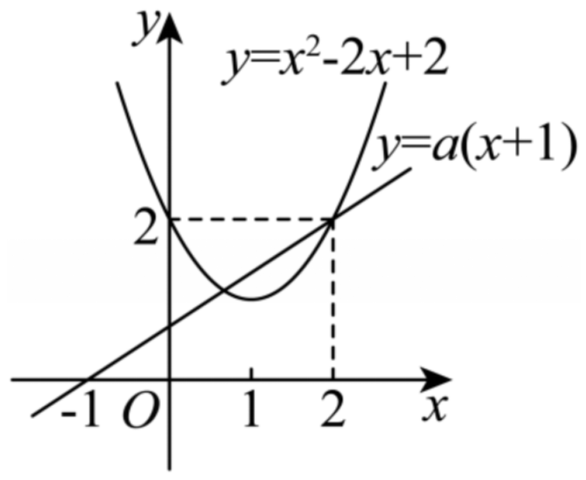
\includegraphics[width=0.30\textwidth]{figures/gao75_q12_graph.png}
\end{center}
% 原卷此处作“≥”，与题干严格不等号方向不一致，照录（见文件头“原卷笔误/存疑”①）
\step{由集合 $A$ 是“$2$ 集合”，故集合 $A$ 中只有一个元素，}
\step{得 $\begin{cases}2^2-2\times2+2\geqslant(2+1)a\\ 1^2-2\times1+2<(1+1)a\end{cases}$，解得 $\dfrac12<a\leqslant\dfrac23$，}
\step{故正实数 $a$ 的取值范围是 $\dfrac12<a\leqslant\dfrac23$.}
\solend
\fi

\end{enumerate}

\bigsec{二、选择题}

\begin{enumerate}
\setcounter{enumi}{12}

\item 已知全集 $U=\R$，集合 $A=\{x\mid x^2<4\}$，$B=\{y\mid y=x^2\}$，则图中阴影部分所表示的集合为\mbox{（\quad）}

\begin{center}
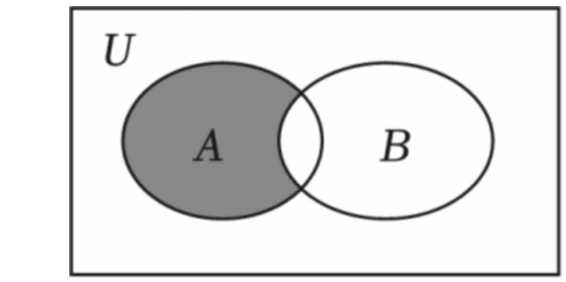
\includegraphics[width=0.26\textwidth]{figures/gao75_q13_venn.png}
\end{center}

\keepwithprev
A. $\{-2,-1,0\}$\qquad B. $(-\infty,4)$\qquad C. $(-2,0)$\qquad D. $(-2,0]$

\ifanswer
\solbegin
\step{集合 $A=\{x\mid x^2<4\}=(-2,2)$，$B=\{y\mid y=x^2\}=[0,+\infty)$，}
\step{图中阴影部分所表示的集合是 $A\cap\overline{B}=(-2,0)$. 故选 $C$.}
\solend
\fi

\item 已知 $x\in\R$，则“$\dfrac1x>1$”是“$x<1$”的\mbox{（\quad）}

\keepwithprev
A. 充分非必要条件\qquad B. 必要非充分条件\qquad C. 充要条件\qquad D. 既非充分又非必要条件

\ifanswer
\solbegin
\step{“$\dfrac1x>1$”$\Leftrightarrow0<x<1$，所以“$\dfrac1x>1$”是“$x<1$”的充分不必要条件. 故选 $A$.}
\solend
\fi

\item 已知集合 $M=\{x\mid x=m+\dfrac16,\,m\in\Z\}$，$N=\{x\mid x=\dfrac n2-\dfrac13,\,n\in\Z\}$，\\
$P=\{x\mid x=\dfrac p2+\dfrac16,\,p\in\Z\}$，则 $M$、$N$、$P$ 的关系为\mbox{（\quad）}

\keepwithprev
A. $M=N\subseteq P$\qquad B. $M\subseteq N=P$\qquad C. $M\subseteq N\subseteq P$\qquad D. $N\subseteq P\subseteq M$

\ifanswer
\solbegin
\step{集合 $N=\{x\mid x=\dfrac n2-\dfrac13,\,n\in\Z\}$，则 $x=\dfrac n2-\dfrac13=\dfrac{3n-2}6$，$n\in\Z$.}
\step{$P=\{x\mid x=\dfrac p2+\dfrac16,\,p\in\Z\}$，则 $x=\dfrac p2+\dfrac16=\dfrac{3p+1}6$，$p\in\Z$.}
\step{$M=\{x\mid x=m+\dfrac16,\,m\in\Z\}$，则 $x=m+\dfrac16=\dfrac{6m+1}6$，$m\in\Z$.}
\step{$M$、$N$、$P$ 三者分母相同，所以只需要比较他们的分子.}
\step{$M$：$6$ 的倍数$+1$，$N=P$：$3$ 的倍数$+1$，所以 $M\subseteq N=P$. 故选 $B$.}
\solend
\fi

\item 设集合 $P_1=\{x\mid x^2+ax+1>0\}$，$P_2=\{x\mid x^2+ax+2>0\}$，$Q_1=\{x\mid x^2+x+b>0\}$，$Q_2=\{x\mid x^2+2x+b>0\}$ 其中 $a,b\in\R$，给出下列两个命题：命题 $q_1$：对任意的 $a$，$P_1$ 是 $P_2$ 的子集；命题 $q_2$：对任意的 $b$，$Q_1$ 不是 $Q_2$ 的子集. 下列说法正确的是\mbox{（\quad）}

\keepwithprev
A. 命题 $q_1$ 是真命题，命题 $q_2$ 是假命题\qquad B. 命题 $q_1$ 是假命题，命题 $q_2$ 是真命题

C. 命题 $q_1$、$q_2$ 都是真命题\qquad D. 命题 $q_1$、$q_2$ 都是假命题

\ifanswer
\solbegin
\step{对于集合 $P_1=\{x\mid x^2+ax+1>0\}$，$P_2=\{x\mid x^2+ax+2>0\}$，}
\step{当 $m\in P_1$，即 $m^2+am+1>0$，得 $m^2+am+2>0$，}
\step{即有 $m\in P_2$，得对任意 $a$，$P_1$ 是 $P_2$ 的子集，命题 $q_1$ 为真命题；}
\step{当 $b=5$ 时，$Q_1=\{x\mid x^2+x+5>0\}=\R$，$Q_2=\{x\mid x^2+2x+5>0\}=\R$，}
\step{得 $Q_1$ 是 $Q_2$ 的子集；}
\step{存在 $b$，使得 $Q_1$ 是 $Q_2$ 的子集，故命题 $q_2$ 是假命题.}
\step{故选 $A$.}
\solend
\fi

\end{enumerate}

\bigsec{三、解答题}

\begin{enumerate}
\setcounter{enumi}{16}

\item 设集合 $A=\{x\mid x^2-2x=0\}$，$B=\{x\mid x^2+2(a+1)x+a^2-1=0\}$.

（1）写出集合 $A$ 的所有子集；

（2）若 $A\cap B=B$，求实数 $a$ 的取值范围.

\ifanswer
\solbegin
\stepm{(1)}{由 $x^2-2x=0$，得 $x=2$ 或 $x=0$，所以 $A=\{0,2\}$，}
\step{故集合 $A$ 的所有子集为 $\varnothing$、$\{0\}$、$\{2\}$、$\{0,2\}$.}
\stepm{(2)}{因为 $A\cap B=B$，所以 $B\subseteq A$，}
\step{方程 $x^2+2(a+1)x+a^2-1=0$，$\Delta=4(a+1)^2-4(a^2-1)=8a+8$，}
\step{若 $\Delta<0$，即 $a<-1$，方程 $x^2+2(a+1)x+a^2-1=0$ 无解，}
\step{此时 $B=\varnothing$，满足题意；}
\step{若 $\Delta=0$，即 $a=-1$，由 $x^2+2(a+1)x+a^2-1=0$，即 $x^2=0$，}
\step{解得 $x=0$，此时 $B=\{0\}$，满足题意；}
\step{若 $\Delta>0$，即 $a>-1$，要使 $B\subseteq A$，}
\step{则方程 $x^2+2(a+1)x+a^2-1=0$ 的解集为 $\{0,2\}$，}
\step{则 $\begin{cases}2+0=-2(a+1)\\ 2\times0=a^2-1\end{cases}$，$a$ 不存在.}
\step{综上所述，$a\leqslant-1$，即实数 $a$ 的取值范围为 $\{a\mid a\leqslant-1\}$.}
\solend
\fi

\ansspace

\item 已知全集 $U=\R$，集合 $A=\left\{x\,\middle|\,\dfrac{x-1}{x-3}<0\right\}$，$B=\{x\mid|x-a|<2\}$.

（1）当 $a=1$ 时，试用区间表示集合 $A$、$B$；

（2）若 $A\cup B=B$，求实数 $a$ 的取值范围.

\ifanswer
\solbegin
\stepm{(1)}{不等式 $\dfrac{x-1}{x-3}<0$ 可化为 $(x-1)(x-3)<0$，解得 $1<x<3$，即 $A=(1,3)$，}
\step{当 $a=1$ 时，$|x-1|<2$，则 $-2<x-1<2$，解得 $-1<x<3$，}
\step{即 $B=(-1,3)$；}
\stepm{(2)}{由不等式 $|x-a|<2$ 得 $-2<x-a<2$，解得 $-2+a<x<2+a$，}
\step{即 $B=\{x\mid-2+a<x<2+a\}$，}
\step{因为 $A\cup B=B$，所以 $A\subseteq B$，则 $\begin{cases}-2+a\leqslant1\\ 2+a\geqslant3\end{cases}$，解得 $1\leqslant a\leqslant3$，}
\step{即实数 $a$ 的取值范围为 $[1,3]$.}
\solend
\fi

\ansspace

\item 法国数学家弗朗索瓦·韦达 1615 年在著作《论方程的识别与订正》中建立了方程根与系数的关系. 发现一元二次方程 $ax^2+bx+c=0$，$a\neq0$ 的根与系数有如下的关系：

$x_1+x_2=-\dfrac ba$，$x_1x_2=\dfrac ca$，此即为韦达定理. 韦达定理的逆定理仍成立：如果两个数 $x_1$，$x_2$ 满足 $x_1+x_2=-\dfrac ba$，$x_1x_2=\dfrac ca$，则这两个数 $x_1$、$x_2$ 是方程 $ax^2+bx+c=0$，$a\neq0$ 的两个根. 例如：$m+n=-3$，$mn=2$，则 $m$、$n$ 是方程 $x^2+3x+2=0$ 的两个根. 请根据上述材料解决以下问题.

（1）已知 $m$、$n$ 是两个不相等的实数，满足 $m^2-6m-5=0$，$n^2-6n-5=0$，求 $\dfrac1m+\dfrac1n$ 的值；

（2）已知实数 $x$、$y$ 满足 $x+y+xy=17$，$x^2y+xy^2=72$，求 $x^2+y^2$ 的值.

\ifanswer
\solbegin
\stepm{(1)}{由题意，不相等的实数 $m$、$n$ 满足 $m^2-6m-5=0$、$n^2-6n-5=0$，}
\step{因此 $m$、$n$ 是一元二次方程 $x^2-6x-5=0$ 的两个不等实根.}
\step{由韦达定理得 $m+n=6$，$mn=-5$，因此 $\dfrac1m+\dfrac1n=\dfrac{m+n}{mn}=\dfrac6{-5}=-\dfrac65$.}
\stepm{(2)}{令 $s=x+y$，$t=xy$，}
\step{因为 $x+y+xy=17$，$x^2y+xy^2=72$，}
\step{即 $x+y+xy=17$，$xy(x+y)=72$，将已知条件变形得 $\begin{cases}s+t=17\\ st=72\end{cases}$.}
\step{由韦达定理逆定理，$s$、$t$ 是一元二次方程 $z^2-17z+72=0$ 的两个实根，}
\step{解方程得 $z_1=8$，$z_2=9$，即有两组解 $\begin{cases}s=8\\ t=9\end{cases}$ 和 $\begin{cases}s=9\\ t=8\end{cases}$.}
\step{当 $\begin{cases}s=8\\ t=9\end{cases}$ 时，$x$、$y$ 是方程 $w^2-8w+9=0$ 的根，}
\step{判别式 $\Delta=8^2-4\times1\times9=64-36=28>0$，符合题意，}
\step{此时 $x^2+y^2=(x+y)^2-2xy=s^2-2t=8^2-2\times9=64-18=46$；}
\step{当 $\begin{cases}s=9\\ t=8\end{cases}$ 时，$x$、$y$ 是方程 $w^2-9w+8=0$ 的根，}
\step{判别式 $\Delta=9^2-4\times1\times8=81-32=49>0$，符合题意，}
\step{此时 $x^2+y^2=(x+y)^2-2xy=s^2-2t=9^2-2\times8=81-16=65$.}
\step{综上，$x^2+y^2$ 的值为 $46$ 或 $65$.}
\solend
\fi

\ansspace

\item 已知关于 $x$ 的不等式 $ax^2-(a+1)x+b<0$.

（1）若不等式的解集是 $\{x\mid1<x<5\}$，求 $a+b$ 的值；

（2）若 $b=-\dfrac12$ 且不等式的解集为 $\R$，求 $a$ 取值范围；

（3）若 $b=1$，讨论此不等式的解集.

\ifanswer
\solbegin
\stepm{(1)}{由题意得 $1$ 和 $5$ 是方程 $ax^2-(a+1)x+b=0$ 的两个根且 $a>0$，}
\step{所以 $1+5=\dfrac{a+1}a$，$1\times5=\dfrac ba$，解得 $a=\dfrac15$，$b=1$，所以 $a+b=\dfrac65$.}
\stepm{(2)}{若 $b=-\dfrac12$，则不等式为 $ax^2-(a+1)x-\dfrac12<0$，}
\step{当 $a\neq0$，则有 $\begin{cases}a<0\\ \Delta=(a+1)^2+2a<0\end{cases}$，解得 $-2-\sqrt3<a<-2+\sqrt3$；}
\step{当 $a=0$，不等式即为 $-x-\dfrac12<0$，则 $x>-\dfrac12$，不合题意；}
\step{所以 $a$ 的取值范围是 $(-2-\sqrt3,-2+\sqrt3)$.}
\stepm{(3)}{若 $b=1$，则不等式为 $ax^2-(a+1)x+1<0$，即 $(ax-1)(x-1)<0$.}
\step{当 $a\neq0$ 时，由 $ax^2-(a+1)x+1<0$ 得 $(ax-1)(x-1)<0$.}
\step{方程 $(ax-1)(x-1)=0$ 的根为 $x=\dfrac1a$ 或 $x=1$，}
\step{当 $0<a<1$ 时，$\dfrac1a>1$，则不等式的解集为 $\left(1,\dfrac1a\right)$；}
\step{当 $a<0$ 时，$\dfrac1a<1$，则不等式的解集为 $\left(-\infty,\dfrac1a\right)\cup(1,+\infty)$；}
\step{当 $a=1$ 时，不等式即为 $(x-1)^2<0$，则不等式的解集为 $\varnothing$；}
\step{当 $a>1$ 时，$\dfrac1a<1$，则不等式的解集为 $\left(\dfrac1a,1\right)$；}
\step{当 $a=0$ 时，不等式为 $-x+1<0$，则不等式的解集为 $(1,+\infty)$；}
\step{综上所述，当 $a<0$ 时，不等式的解集为 $\left(-\infty,\dfrac1a\right)\cup(1,+\infty)$；}
\step{当 $a=0$ 时，不等式的解集为 $(1,+\infty)$；}
\step{当 $0<a<1$ 时，不等式的解集为 $\left(1,\dfrac1a\right)$；}
\step{当 $a=1$ 时，不等式的解集为 $\varnothing$；}
\step{当 $a>1$ 时，不等式的解集为 $\left(\dfrac1a,1\right)$.}
\solend
\fi

\ansspace

\item 已知关于 $x$ 的不等式① $x^2+2cx+c>0$，② $x^2+cx+c^2-1>0$，其中 $c$ 是实数.

（1）若 $1$ 是不等式②的一个解，求实数 $c$ 的取值范围；

（2）证明：不等式①、②中至多有一个恒成立；

（3）当 $c=0$ 时，“$x$ 满足 $|mx^2-4x+3|>5$”的一个必要非充分条件是“$x$ 满足 $x^2+cx+c^2-1>0$，求实数 $m$ 的取值范围.

\ifanswer
\solbegin
\stepm{(1)}{因为 $1$ 是不等式②的一个解，所以 $1+c+c^2-1>0$，}
\step{即 $c(c+1)>0$，解得 $c>0$ 或 $c<-1$，}
\step{所以实数 $c$ 的取值范围为 $(-\infty,-1)\cup(0,+\infty)$.}
\stepm{(2)}{假设不等式①、②都恒成立，}
\step{不等式① $x^2+2cx+c>0$ 恒成立，所以 $4c^2-4c<0$，所以 $0<c<1$；}
\step{② $x^2+cx+c^2-1>0$ 恒成立，所以 $c^2-4(c^2-1)<0$，$c^2>\dfrac43$，}
\step{解得 $c>\dfrac{2\sqrt3}3$ 或 $c<-\dfrac{2\sqrt3}3$；}
\step{所以当不等式①、②都恒成立时，}
\step{不等式组 $\begin{cases}0<c<1\\ c\in\left(-\infty,-\dfrac{2\sqrt3}3\right)\cup\left(\dfrac{2\sqrt3}3,+\infty\right)\end{cases}$ 无解，}
\step{所以假设不成立，}
\step{所以不等式①、②中至多有一个恒成立.}
\stepm{(3)}{当 $c=0$ 时，由 $x^2+cx+c^2-1>0$ 得 $x^2-1>0$，}
\step{解集为 $(-\infty,-1)\cup(1,+\infty)$.}
\step{记集合 $A=\{x\mid|mx^2-4x+3|>5\}$，集合 $B=\{x\mid x<-1\text{ 或 }x>1\}$.}
\step{由“$x$ 满足 $|mx^2-4x+3|>5$”的一个必要非充分条件是}
\step{“$x$ 满足 $x^2+cx+c^2-1>0$”得 $A$ 是 $B$ 的真子集.}
\step{所以 $\overline{B}$ 是 $A$ 的真子集，即对任意 $x\in[-1,1]$，$|mx^2-4x+3|\leqslant5$ 恒成立.}
\step{当 $x=0$ 时，不等式 $-5\leqslant mx^2-4x+3\leqslant5$ 恒成立；}
\step{当 $x\in[-1,0)\cup(0,1]$ 时，}
\step{则 $mx^2-4x+3\geqslant-5$ 与 $mx^2-4x+3\leqslant5$ 同时成立.}
\step{①由 $mx^2-4x+3\geqslant-5$，得 $m\geqslant\dfrac{4x-8}{x^2}$，求值域得 $\dfrac{4x-8}{x^2}$ 的最大值 $=-4$，}
\step{所以 $m\geqslant-4$.}
\step{②由 $mx^2-4x+3\leqslant5$，得 $m\leqslant\dfrac{4x+2}{x^2}$，求值域得 $\dfrac{4x+2}{x^2}$ 的最小值 $=-2$，}
\step{所以 $m\leqslant-2$.}
\step{综上所述，实数 $m$ 的取值范围为 $[-4,-2]$.}
\solend
\fi

\ansspace*[7]

\end{enumerate}

\end{document}
"
% 紧凑版：xelatex "\def\iscompact{1}% 高一75_市二中学_10月月考.tex
%   —— 高一上数学“2026-2027 年市二中学高一上 10 月月考”（讲评版）
% 试卷版：xelatex 高一75_市二中学_10月月考.tex
% 答案版：xelatex "\def\isanswer{1}% 高一75_市二中学_10月月考.tex
%   —— 高一上数学“2026-2027 年市二中学高一上 10 月月考”（讲评版）
% 试卷版：xelatex 高一75_市二中学_10月月考.tex
% 答案版：xelatex "\def\isanswer{1}\input{高一75_市二中学_10月月考.tex}"
% 紧凑版：xelatex "\def\iscompact{1}\input{高一75_市二中学_10月月考.tex}"
%
% 原始材料：微信公众号“魔都数学加油站”文章，连载“27学年高一75”；
% 原文标题“27学年高一75——2026-2027年上海市市二中学高一上10月月考”；
% 原文链接：https://mp.weixin.qq.com/s/dhxtwWEZgKLxeKdkbWqOhw。
% 页面标注发布时间 2026-10-22 21:45（上海）。
% 正文为 11 张 PNG 页（`原图/高一75_市二中学_10月月考/01..11.png`）：
% 第 2、4、5、6、9 页为 4762×6735，其余 6 页为 2560×3620，均按页序读取。
% 11 页全为试卷正文页（卷首标题在第 1 页页顶，卷末第 21 题 (3) 解析止于第 11 页），
% 无封面页、目录页、二维码或宣传页。粉色斜排“魔都数学加油站”为卷面水印，未录入。
%
% 卷首标题：照卷面印作“2026-2027 年市二中学高一上 10 月月考”（黑体加粗一行）。
% 原卷年份区间用半角连字符，本稿按全稿惯例排 en dash；原卷无副标题。
%
% 篇幅与题号：原卷自第 3 题起编号（第 1、2 题不在本卷内）。填空题 3—12（10 题）、
% 选择题 13—16（4 题）、解答题 17—21（5 题），共 19 题。本稿沿用原节与原题号，
% 只改排为全稿统一的大节样式。
%
% 讲评版：原卷第 4 题只印【答案】（“$[-1,2]$”），本稿只给 \ans{}；其余 18 题均印
% 【解析】，用 \solbegin…\solend。四道选择题的作答括号原卷即留空，答案写在解析末句
% “故选 C／A／B／A”，照录在解析内，不另提 \ans{}。
%
% 副标题：原卷未印副标题。本稿按“知识模块”口径标作“集合与常用逻辑用语、不等式”：
% 19 题中集合与常用逻辑用语 9 题（第 3、4、5、8、10、12、13、15、17、18 题中的集合题），
% 不等式 10 题（第 6、7、9、11、19、20、21 题及第 12、20 题的不等式部分），两类均确有
% 分量，故并标。口径同 高一63、高一68—74。
%
% 与原卷的排版差异：
%   ① 原卷每题下直接印【答案】/【解析】，本稿按全稿惯例将答案与解析置于答案版；
%   ② 原卷未印副标题，本稿按“知识模块”口径补出；
%   ③ 原卷填空横线约四个字宽，本稿按全稿惯例统一排 \blankline[4.4em]；
%   ④ 原卷数集记号排粗体 $\mathbf{R}$（第 5、6、7、9、10、14、18、20、21 题），本稿
%      按全稿惯例改用 $\R$（同 高一68—74）；第 11 题的“解集为 $\R$”同此；
%   ⑤ 原卷句末标点多为西文句点，均逐处照录；
%   ⑥ 第 17—21 题的子问原卷印作“（1）…（2）…”，本稿按 高一69—74 成例用行内
%      “（1）（2）（3）”段，解析中的子问标号用 \stepm{(1)}{…}；
%   ⑦ 每道解答题原卷未留作答空白，本稿按全稿惯例加 \ansspace（末题用 \ansspace*）；
%   ⑧ 选择题的作答括号原卷排半角“(    )”，本稿按全稿惯例排 \mbox{（\quad）}；
%      选项行排照原卷——第 13、14 题一行四条，第 15、16 题一行四条；
%   ⑨ 第 9、12、15、17—21 题解析中的不等式组／方程组，原卷均排作“{”连接的多行式，
%      本稿按全稿惯例排 cases；
%   ⑩ 第 12 题解析有一幅“抛物线 + 直线”图：原卷印在解析第 3 行右侧、题干无“如图”二字
%      （解析里写“两函数图象如图：”）。本稿按原卷截图裁取（`figures/gao75_q12_graph.png`，
%      由第 3 页原图裁出、去除粉色水印后转灰度，未放大），放在答案版解析第 3 条之后；
%   ⑪ 第 13 题题干中间有一幅韦恩图（全集矩形内含 A、B 两圆，A 涂灰）：原卷印在题干
%      右侧、题干句子被图隔开。本稿按原卷截图裁取（`figures/gao75_q13_venn.png`，由第 3
%      页原图裁出、去除粉色水印后转灰度，并抹去左侧侵入的“分”字），放在题干之后、
%      选项之前，仅答案版出。
%
% 原卷笔误/存疑（均照录未改，正文对应处另有 % 注）：
%   ① 第 12 题解析列不等式组时写 $2^2-2\times2+2\geqslant(2+1)a$，与
%      $x^2-2x+2<a(x+1)$ 的严格不等号方向不一致；原卷如此，照录未改。
%   ② 第 14 题选项 A—D 的“充分非必要”“必要非充分”“既非充分又非必要”与原卷
%      其它题的“充分不必要”写法不同，照录未统一。
%   ④ 第 21 题 (3) 题干的“$x$ 满足 $|mx^2-4x+3|>5$”的一个必要非充分条件是
%      “$x$ 满足 $x^2+cx+c^2-1>0$，原卷只有左引号、无右引号（且逗号在引号内），
%      本稿照录未补。
%   ③ 第 20 题 (2) 的解集写成 $(-2-\sqrt3,-2+\sqrt3)$，其中 $a<0$ 与 $\Delta<0$ 联立后
%      左端点应为 $-2-\sqrt3$、右端点为 $-2+\sqrt3$；原卷如此，照录未改。
%
% 行数核对：逐题数 \step/\stepm 条数与原卷【解析】印刷行数，18 题逐一相符，
% 合计 132 条 / 132 行（Q3：6；Q5：1；Q6：2；Q7：1；Q8：2；Q9：3；Q10：10；
% Q11：8；Q12：6；Q13：2；Q14：1；Q15：5；Q16：7；Q17：12；Q18：7；Q19：15；
% Q20：19；Q21：25）。另第 4 题只印【答案】，提 \ans{}，不计入 \step 账。
%
% 插图：第 12 题解析的抛物线图、第 13 题题干的韦恩图，见上⑩⑪；其余题干无配图。
%
\documentclass[a4paper,11pt]{article}
\usepackage{common}

\begin{document}

\examtitlest[3]{2026--2027 年市二中学高一上 10 月月考}{集合与常用逻辑用语、不等式}

\bigsec{一、填空题}

\begin{enumerate}
\setcounter{enumi}{2}

\item 已知集合 $A=\{a,a^2\}$，且 $1\in A$，则 $a=$\blankline[4.4em].

\ifanswer
\solbegin
\step{因为 $1\in A=\{a,a^2\}$，所以 $a=1$ 或 $a^2=1$.}
\step{又集合 $A=\{a,a^2\}$ 是用列举法写出两个元素的，其元素必须互异，故 $a\neq a^2$，}
\step{即 $a\neq0$ 且 $a\neq1$，所以 $a=1$ 应舍去；}
\step{由 $a^2=1$ 得 $a=1$（舍去）或 $a=-1$.}
\step{当 $a=-1$ 时，$A=\{-1,1\}$，满足 $1\in A$ 且两个元素互异.}
\step{故 $a=-1$.}
\solend
\fi

\item 已知集合 $A=[-1,1]$，$B=[0,2]$，则 $A\cup B=$\blankline[4.4em].

\ifanswer
\ans{$[-1,2]$}
\fi

\item 已知全集 $U=\R$，集合 $A=\{x\mid x\neq1\}$，则 $\overline{A}=$\blankline[4.4em].

\ifanswer
\solbegin
\step{因为全集 $U=\R$，集合 $A=\{x\mid x\neq1\}$，所以 $\overline{A}=\{x\mid x=1\}$.}
\solend
\fi

\item 设 $x\in\R$，不等式 $x^2-4x<0$ 的解集用区间表示是\blankline[4.4em].

\ifanswer
\solbegin
\step{因为 $x^2-4x<0$，即 $x(x-4)<0$，所以 $0<x<4$，}
\step{所以 $x(x-4)<0$ 的解集为 $(0,4)$.}
\solend
\fi

\item 已知 $m\in\R$，若关于 $x$ 的方程 $2mx^2+3x+m-1=m^2\cdot x^2+(m+1)x+1$ 解集为 $\R$，则 $m$ 的值为\blankline[4.4em].

\ifanswer
\solbegin
\step{由题意得 $2m=m^2$，$3=m+1$，$m-1=1$，所以 $m=2$.}
\solend
\fi

\item 设 $\alpha:x\leqslant m$，$\beta:|x-2|\leqslant1$，若 $\alpha$ 是 $\beta$ 的必要条件，则实数 $m$ 的取值范围是\blankline[4.4em].

\ifanswer
\solbegin
\step{由 $|x-2|\leqslant1$，得 $-1\leqslant x-2\leqslant1$，解得 $1\leqslant x\leqslant3$，}
\step{因为 $\alpha$ 是 $\beta$ 的必要条件，所以 $\{x\mid1\leqslant x\leqslant3\}\subseteq\{x\mid x\leqslant m\}$，得 $m\geqslant3$.}
\solend
\fi

\item 设 $a\in\R$，若关于 $x$ 的不等式 $\dfrac{a}{x-1}\leqslant1$ 的解集是 $(-\infty,1)\cup[2,+\infty)$，则 $a$ 的值为\blankline[4.4em].

\ifanswer
\solbegin
\step{不等式可变形为 $\dfrac{a+1-x}{x-1}\leqslant0$，等价于 $\begin{cases}(a+1-x)(x-1)\leqslant0\\ x-1\neq0\end{cases}$，}
\step{因为原不等式的解集是 $(-\infty,1)\cup[2,+\infty)$，}
\step{所以 $1$，$2$ 是方程 $(a+1-x)(x-1)=0$ 的两根，所以 $a+1=2$，解得 $a=1$.}
\solend
\fi

\item 下列命题：① “$x>1$ 或 $y>1$”的否定形式是“$x\leqslant1$ 或 $y\leqslant1$”，② 若 $A\cup B=B$，则 $A\subseteq B$，③ 方程 $ax+1=0$ 的解是 $x=-\frac1a$，④ “$ac=bc$”是“$a=b$”的必要非充分条件，⑤ “任意 $x\in\R$，$f(x)=f(-x)$”的否定形式是“存在 $x_0\in\R$，使得 $f(x_0)\neq f(-x_0)$”其中真命题的序号是\blankline[4.4em]（填写序号）.

\ifanswer
\solbegin
\step{①假命题：“$x>1$ 或 $y>1$”的否定形式是“$x\leqslant1$ 且 $y\leqslant1$”；}
\step{②真命题：$A\cup B=B\Leftrightarrow A\subseteq B$；}
\step{③假命题：当 $a=0$ 时，方程无解，因此该命题忽略了 $a=0$ 的情况；}
\step{④真命题：先判断必要性：若 $a=b$，则有 $ac=bc$，所以必要性成立；}
\step{再判断充分性：若 $ac=bc$，即 $(a-b)c=0$，当 $c=0$ 时，$a$ 和 $b$ 可以不相等，}
\step{因此充分性不成立.}
\step{⑤真命题：全称命题的否定是存在量词命题，}
\step{“任意 $x\in\R$，$f(x)=f(-x)$”的否定形式是}
\step{“存在 $x_0\in\R$，使得 $f(x_0)\neq f(-x_0)$”，表述正确.}
\step{故正确的是②④⑤.}
\solend
\fi

\item 为了加强家校联系，蔡老师组建了一个由学生、家长和教师组成的微信群. 已知该群中男学生人数多于女学生人数，女学生人数多于家长人数，家长人数多于教师人数，教师人数的两倍多于男学生人数. 则该微信群人数的最小值为\blankline[4.4em].

\ifanswer
\solbegin
\step{设男学生、女学生、家长、教师的人数分别为 $M$、$F$、$P$、$T$，}
\step{它们都是正整数.}
\step{由题意得 $M>F>P>T$，且教师人数的两倍多于男学生人数，即 $2T>M$.}
\step{由 $M>F>P>T$ 得 $M\geqslant T+3$；}
\step{又 $2T>M\geqslant T+3$，所以 $2T>T+3$，解得 $T>3$，故教师人数最少为 $T=4$.}
\step{当 $T=4$ 时，为使总人数最少，取 $P=5$、$F=6$、$M=7$，}
\step{此时 $7>6>5>4$ 且 $2\times4=8>7$，满足题意.}
\step{于是微信群人数为 $4+5+6+7=22$，所以该微信群人数的最小值为 $22$.}
\solend
\fi

\item 若集合 $M$ 有 $k$ 个子集，则称集合 $M$ 为“$k$ 集合”，\\
已知集合 $A=\{x\mid x^2-(a+2)x+2-a<0,\,x\in\Z\}$ 是“$2$ 集合”，则正实数 $a$ 的取值范围是\blankline[4.4em].

\ifanswer
\solbegin
\step{由 $x^2-(a+2)x+2-a<0$，得 $x^2-2x+2<a(x+1)$，}
\step{设二次函数 $y=x^2-2x+2$ 与一次函数 $y=a(x+1)$，}
\needvspace{13\baselineskip}
\step{由 $a>0$，$y=a(x+1)$ 过定点 $(-1,0)$，两函数图象如图：}
\begin{center}
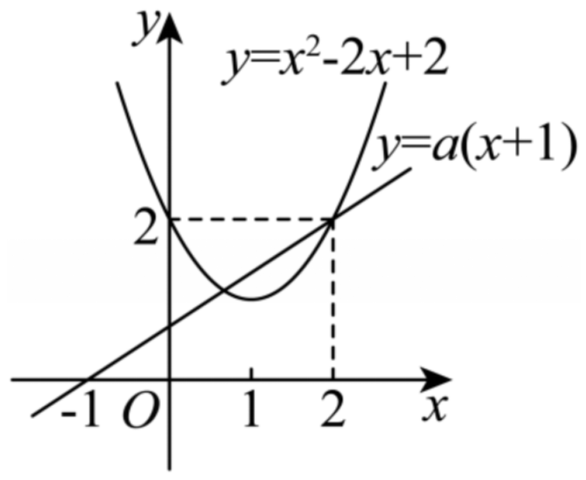
\includegraphics[width=0.30\textwidth]{figures/gao75_q12_graph.png}
\end{center}
% 原卷此处作“≥”，与题干严格不等号方向不一致，照录（见文件头“原卷笔误/存疑”①）
\step{由集合 $A$ 是“$2$ 集合”，故集合 $A$ 中只有一个元素，}
\step{得 $\begin{cases}2^2-2\times2+2\geqslant(2+1)a\\ 1^2-2\times1+2<(1+1)a\end{cases}$，解得 $\dfrac12<a\leqslant\dfrac23$，}
\step{故正实数 $a$ 的取值范围是 $\dfrac12<a\leqslant\dfrac23$.}
\solend
\fi

\end{enumerate}

\bigsec{二、选择题}

\begin{enumerate}
\setcounter{enumi}{12}

\item 已知全集 $U=\R$，集合 $A=\{x\mid x^2<4\}$，$B=\{y\mid y=x^2\}$，则图中阴影部分所表示的集合为\mbox{（\quad）}

\begin{center}
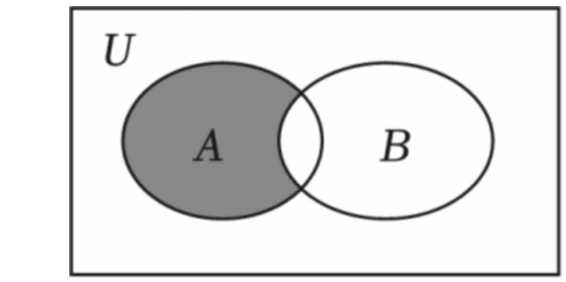
\includegraphics[width=0.26\textwidth]{figures/gao75_q13_venn.png}
\end{center}

\keepwithprev
A. $\{-2,-1,0\}$\qquad B. $(-\infty,4)$\qquad C. $(-2,0)$\qquad D. $(-2,0]$

\ifanswer
\solbegin
\step{集合 $A=\{x\mid x^2<4\}=(-2,2)$，$B=\{y\mid y=x^2\}=[0,+\infty)$，}
\step{图中阴影部分所表示的集合是 $A\cap\overline{B}=(-2,0)$. 故选 $C$.}
\solend
\fi

\item 已知 $x\in\R$，则“$\dfrac1x>1$”是“$x<1$”的\mbox{（\quad）}

\keepwithprev
A. 充分非必要条件\qquad B. 必要非充分条件\qquad C. 充要条件\qquad D. 既非充分又非必要条件

\ifanswer
\solbegin
\step{“$\dfrac1x>1$”$\Leftrightarrow0<x<1$，所以“$\dfrac1x>1$”是“$x<1$”的充分不必要条件. 故选 $A$.}
\solend
\fi

\item 已知集合 $M=\{x\mid x=m+\dfrac16,\,m\in\Z\}$，$N=\{x\mid x=\dfrac n2-\dfrac13,\,n\in\Z\}$，\\
$P=\{x\mid x=\dfrac p2+\dfrac16,\,p\in\Z\}$，则 $M$、$N$、$P$ 的关系为\mbox{（\quad）}

\keepwithprev
A. $M=N\subseteq P$\qquad B. $M\subseteq N=P$\qquad C. $M\subseteq N\subseteq P$\qquad D. $N\subseteq P\subseteq M$

\ifanswer
\solbegin
\step{集合 $N=\{x\mid x=\dfrac n2-\dfrac13,\,n\in\Z\}$，则 $x=\dfrac n2-\dfrac13=\dfrac{3n-2}6$，$n\in\Z$.}
\step{$P=\{x\mid x=\dfrac p2+\dfrac16,\,p\in\Z\}$，则 $x=\dfrac p2+\dfrac16=\dfrac{3p+1}6$，$p\in\Z$.}
\step{$M=\{x\mid x=m+\dfrac16,\,m\in\Z\}$，则 $x=m+\dfrac16=\dfrac{6m+1}6$，$m\in\Z$.}
\step{$M$、$N$、$P$ 三者分母相同，所以只需要比较他们的分子.}
\step{$M$：$6$ 的倍数$+1$，$N=P$：$3$ 的倍数$+1$，所以 $M\subseteq N=P$. 故选 $B$.}
\solend
\fi

\item 设集合 $P_1=\{x\mid x^2+ax+1>0\}$，$P_2=\{x\mid x^2+ax+2>0\}$，$Q_1=\{x\mid x^2+x+b>0\}$，$Q_2=\{x\mid x^2+2x+b>0\}$ 其中 $a,b\in\R$，给出下列两个命题：命题 $q_1$：对任意的 $a$，$P_1$ 是 $P_2$ 的子集；命题 $q_2$：对任意的 $b$，$Q_1$ 不是 $Q_2$ 的子集. 下列说法正确的是\mbox{（\quad）}

\keepwithprev
A. 命题 $q_1$ 是真命题，命题 $q_2$ 是假命题\qquad B. 命题 $q_1$ 是假命题，命题 $q_2$ 是真命题

C. 命题 $q_1$、$q_2$ 都是真命题\qquad D. 命题 $q_1$、$q_2$ 都是假命题

\ifanswer
\solbegin
\step{对于集合 $P_1=\{x\mid x^2+ax+1>0\}$，$P_2=\{x\mid x^2+ax+2>0\}$，}
\step{当 $m\in P_1$，即 $m^2+am+1>0$，得 $m^2+am+2>0$，}
\step{即有 $m\in P_2$，得对任意 $a$，$P_1$ 是 $P_2$ 的子集，命题 $q_1$ 为真命题；}
\step{当 $b=5$ 时，$Q_1=\{x\mid x^2+x+5>0\}=\R$，$Q_2=\{x\mid x^2+2x+5>0\}=\R$，}
\step{得 $Q_1$ 是 $Q_2$ 的子集；}
\step{存在 $b$，使得 $Q_1$ 是 $Q_2$ 的子集，故命题 $q_2$ 是假命题.}
\step{故选 $A$.}
\solend
\fi

\end{enumerate}

\bigsec{三、解答题}

\begin{enumerate}
\setcounter{enumi}{16}

\item 设集合 $A=\{x\mid x^2-2x=0\}$，$B=\{x\mid x^2+2(a+1)x+a^2-1=0\}$.

（1）写出集合 $A$ 的所有子集；

（2）若 $A\cap B=B$，求实数 $a$ 的取值范围.

\ifanswer
\solbegin
\stepm{(1)}{由 $x^2-2x=0$，得 $x=2$ 或 $x=0$，所以 $A=\{0,2\}$，}
\step{故集合 $A$ 的所有子集为 $\varnothing$、$\{0\}$、$\{2\}$、$\{0,2\}$.}
\stepm{(2)}{因为 $A\cap B=B$，所以 $B\subseteq A$，}
\step{方程 $x^2+2(a+1)x+a^2-1=0$，$\Delta=4(a+1)^2-4(a^2-1)=8a+8$，}
\step{若 $\Delta<0$，即 $a<-1$，方程 $x^2+2(a+1)x+a^2-1=0$ 无解，}
\step{此时 $B=\varnothing$，满足题意；}
\step{若 $\Delta=0$，即 $a=-1$，由 $x^2+2(a+1)x+a^2-1=0$，即 $x^2=0$，}
\step{解得 $x=0$，此时 $B=\{0\}$，满足题意；}
\step{若 $\Delta>0$，即 $a>-1$，要使 $B\subseteq A$，}
\step{则方程 $x^2+2(a+1)x+a^2-1=0$ 的解集为 $\{0,2\}$，}
\step{则 $\begin{cases}2+0=-2(a+1)\\ 2\times0=a^2-1\end{cases}$，$a$ 不存在.}
\step{综上所述，$a\leqslant-1$，即实数 $a$ 的取值范围为 $\{a\mid a\leqslant-1\}$.}
\solend
\fi

\ansspace

\item 已知全集 $U=\R$，集合 $A=\left\{x\,\middle|\,\dfrac{x-1}{x-3}<0\right\}$，$B=\{x\mid|x-a|<2\}$.

（1）当 $a=1$ 时，试用区间表示集合 $A$、$B$；

（2）若 $A\cup B=B$，求实数 $a$ 的取值范围.

\ifanswer
\solbegin
\stepm{(1)}{不等式 $\dfrac{x-1}{x-3}<0$ 可化为 $(x-1)(x-3)<0$，解得 $1<x<3$，即 $A=(1,3)$，}
\step{当 $a=1$ 时，$|x-1|<2$，则 $-2<x-1<2$，解得 $-1<x<3$，}
\step{即 $B=(-1,3)$；}
\stepm{(2)}{由不等式 $|x-a|<2$ 得 $-2<x-a<2$，解得 $-2+a<x<2+a$，}
\step{即 $B=\{x\mid-2+a<x<2+a\}$，}
\step{因为 $A\cup B=B$，所以 $A\subseteq B$，则 $\begin{cases}-2+a\leqslant1\\ 2+a\geqslant3\end{cases}$，解得 $1\leqslant a\leqslant3$，}
\step{即实数 $a$ 的取值范围为 $[1,3]$.}
\solend
\fi

\ansspace

\item 法国数学家弗朗索瓦·韦达 1615 年在著作《论方程的识别与订正》中建立了方程根与系数的关系. 发现一元二次方程 $ax^2+bx+c=0$，$a\neq0$ 的根与系数有如下的关系：

$x_1+x_2=-\dfrac ba$，$x_1x_2=\dfrac ca$，此即为韦达定理. 韦达定理的逆定理仍成立：如果两个数 $x_1$，$x_2$ 满足 $x_1+x_2=-\dfrac ba$，$x_1x_2=\dfrac ca$，则这两个数 $x_1$、$x_2$ 是方程 $ax^2+bx+c=0$，$a\neq0$ 的两个根. 例如：$m+n=-3$，$mn=2$，则 $m$、$n$ 是方程 $x^2+3x+2=0$ 的两个根. 请根据上述材料解决以下问题.

（1）已知 $m$、$n$ 是两个不相等的实数，满足 $m^2-6m-5=0$，$n^2-6n-5=0$，求 $\dfrac1m+\dfrac1n$ 的值；

（2）已知实数 $x$、$y$ 满足 $x+y+xy=17$，$x^2y+xy^2=72$，求 $x^2+y^2$ 的值.

\ifanswer
\solbegin
\stepm{(1)}{由题意，不相等的实数 $m$、$n$ 满足 $m^2-6m-5=0$、$n^2-6n-5=0$，}
\step{因此 $m$、$n$ 是一元二次方程 $x^2-6x-5=0$ 的两个不等实根.}
\step{由韦达定理得 $m+n=6$，$mn=-5$，因此 $\dfrac1m+\dfrac1n=\dfrac{m+n}{mn}=\dfrac6{-5}=-\dfrac65$.}
\stepm{(2)}{令 $s=x+y$，$t=xy$，}
\step{因为 $x+y+xy=17$，$x^2y+xy^2=72$，}
\step{即 $x+y+xy=17$，$xy(x+y)=72$，将已知条件变形得 $\begin{cases}s+t=17\\ st=72\end{cases}$.}
\step{由韦达定理逆定理，$s$、$t$ 是一元二次方程 $z^2-17z+72=0$ 的两个实根，}
\step{解方程得 $z_1=8$，$z_2=9$，即有两组解 $\begin{cases}s=8\\ t=9\end{cases}$ 和 $\begin{cases}s=9\\ t=8\end{cases}$.}
\step{当 $\begin{cases}s=8\\ t=9\end{cases}$ 时，$x$、$y$ 是方程 $w^2-8w+9=0$ 的根，}
\step{判别式 $\Delta=8^2-4\times1\times9=64-36=28>0$，符合题意，}
\step{此时 $x^2+y^2=(x+y)^2-2xy=s^2-2t=8^2-2\times9=64-18=46$；}
\step{当 $\begin{cases}s=9\\ t=8\end{cases}$ 时，$x$、$y$ 是方程 $w^2-9w+8=0$ 的根，}
\step{判别式 $\Delta=9^2-4\times1\times8=81-32=49>0$，符合题意，}
\step{此时 $x^2+y^2=(x+y)^2-2xy=s^2-2t=9^2-2\times8=81-16=65$.}
\step{综上，$x^2+y^2$ 的值为 $46$ 或 $65$.}
\solend
\fi

\ansspace

\item 已知关于 $x$ 的不等式 $ax^2-(a+1)x+b<0$.

（1）若不等式的解集是 $\{x\mid1<x<5\}$，求 $a+b$ 的值；

（2）若 $b=-\dfrac12$ 且不等式的解集为 $\R$，求 $a$ 取值范围；

（3）若 $b=1$，讨论此不等式的解集.

\ifanswer
\solbegin
\stepm{(1)}{由题意得 $1$ 和 $5$ 是方程 $ax^2-(a+1)x+b=0$ 的两个根且 $a>0$，}
\step{所以 $1+5=\dfrac{a+1}a$，$1\times5=\dfrac ba$，解得 $a=\dfrac15$，$b=1$，所以 $a+b=\dfrac65$.}
\stepm{(2)}{若 $b=-\dfrac12$，则不等式为 $ax^2-(a+1)x-\dfrac12<0$，}
\step{当 $a\neq0$，则有 $\begin{cases}a<0\\ \Delta=(a+1)^2+2a<0\end{cases}$，解得 $-2-\sqrt3<a<-2+\sqrt3$；}
\step{当 $a=0$，不等式即为 $-x-\dfrac12<0$，则 $x>-\dfrac12$，不合题意；}
\step{所以 $a$ 的取值范围是 $(-2-\sqrt3,-2+\sqrt3)$.}
\stepm{(3)}{若 $b=1$，则不等式为 $ax^2-(a+1)x+1<0$，即 $(ax-1)(x-1)<0$.}
\step{当 $a\neq0$ 时，由 $ax^2-(a+1)x+1<0$ 得 $(ax-1)(x-1)<0$.}
\step{方程 $(ax-1)(x-1)=0$ 的根为 $x=\dfrac1a$ 或 $x=1$，}
\step{当 $0<a<1$ 时，$\dfrac1a>1$，则不等式的解集为 $\left(1,\dfrac1a\right)$；}
\step{当 $a<0$ 时，$\dfrac1a<1$，则不等式的解集为 $\left(-\infty,\dfrac1a\right)\cup(1,+\infty)$；}
\step{当 $a=1$ 时，不等式即为 $(x-1)^2<0$，则不等式的解集为 $\varnothing$；}
\step{当 $a>1$ 时，$\dfrac1a<1$，则不等式的解集为 $\left(\dfrac1a,1\right)$；}
\step{当 $a=0$ 时，不等式为 $-x+1<0$，则不等式的解集为 $(1,+\infty)$；}
\step{综上所述，当 $a<0$ 时，不等式的解集为 $\left(-\infty,\dfrac1a\right)\cup(1,+\infty)$；}
\step{当 $a=0$ 时，不等式的解集为 $(1,+\infty)$；}
\step{当 $0<a<1$ 时，不等式的解集为 $\left(1,\dfrac1a\right)$；}
\step{当 $a=1$ 时，不等式的解集为 $\varnothing$；}
\step{当 $a>1$ 时，不等式的解集为 $\left(\dfrac1a,1\right)$.}
\solend
\fi

\ansspace

\item 已知关于 $x$ 的不等式① $x^2+2cx+c>0$，② $x^2+cx+c^2-1>0$，其中 $c$ 是实数.

（1）若 $1$ 是不等式②的一个解，求实数 $c$ 的取值范围；

（2）证明：不等式①、②中至多有一个恒成立；

（3）当 $c=0$ 时，“$x$ 满足 $|mx^2-4x+3|>5$”的一个必要非充分条件是“$x$ 满足 $x^2+cx+c^2-1>0$，求实数 $m$ 的取值范围.

\ifanswer
\solbegin
\stepm{(1)}{因为 $1$ 是不等式②的一个解，所以 $1+c+c^2-1>0$，}
\step{即 $c(c+1)>0$，解得 $c>0$ 或 $c<-1$，}
\step{所以实数 $c$ 的取值范围为 $(-\infty,-1)\cup(0,+\infty)$.}
\stepm{(2)}{假设不等式①、②都恒成立，}
\step{不等式① $x^2+2cx+c>0$ 恒成立，所以 $4c^2-4c<0$，所以 $0<c<1$；}
\step{② $x^2+cx+c^2-1>0$ 恒成立，所以 $c^2-4(c^2-1)<0$，$c^2>\dfrac43$，}
\step{解得 $c>\dfrac{2\sqrt3}3$ 或 $c<-\dfrac{2\sqrt3}3$；}
\step{所以当不等式①、②都恒成立时，}
\step{不等式组 $\begin{cases}0<c<1\\ c\in\left(-\infty,-\dfrac{2\sqrt3}3\right)\cup\left(\dfrac{2\sqrt3}3,+\infty\right)\end{cases}$ 无解，}
\step{所以假设不成立，}
\step{所以不等式①、②中至多有一个恒成立.}
\stepm{(3)}{当 $c=0$ 时，由 $x^2+cx+c^2-1>0$ 得 $x^2-1>0$，}
\step{解集为 $(-\infty,-1)\cup(1,+\infty)$.}
\step{记集合 $A=\{x\mid|mx^2-4x+3|>5\}$，集合 $B=\{x\mid x<-1\text{ 或 }x>1\}$.}
\step{由“$x$ 满足 $|mx^2-4x+3|>5$”的一个必要非充分条件是}
\step{“$x$ 满足 $x^2+cx+c^2-1>0$”得 $A$ 是 $B$ 的真子集.}
\step{所以 $\overline{B}$ 是 $A$ 的真子集，即对任意 $x\in[-1,1]$，$|mx^2-4x+3|\leqslant5$ 恒成立.}
\step{当 $x=0$ 时，不等式 $-5\leqslant mx^2-4x+3\leqslant5$ 恒成立；}
\step{当 $x\in[-1,0)\cup(0,1]$ 时，}
\step{则 $mx^2-4x+3\geqslant-5$ 与 $mx^2-4x+3\leqslant5$ 同时成立.}
\step{①由 $mx^2-4x+3\geqslant-5$，得 $m\geqslant\dfrac{4x-8}{x^2}$，求值域得 $\dfrac{4x-8}{x^2}$ 的最大值 $=-4$，}
\step{所以 $m\geqslant-4$.}
\step{②由 $mx^2-4x+3\leqslant5$，得 $m\leqslant\dfrac{4x+2}{x^2}$，求值域得 $\dfrac{4x+2}{x^2}$ 的最小值 $=-2$，}
\step{所以 $m\leqslant-2$.}
\step{综上所述，实数 $m$ 的取值范围为 $[-4,-2]$.}
\solend
\fi

\ansspace*[7]

\end{enumerate}

\end{document}
"
% 紧凑版：xelatex "\def\iscompact{1}% 高一75_市二中学_10月月考.tex
%   —— 高一上数学“2026-2027 年市二中学高一上 10 月月考”（讲评版）
% 试卷版：xelatex 高一75_市二中学_10月月考.tex
% 答案版：xelatex "\def\isanswer{1}\input{高一75_市二中学_10月月考.tex}"
% 紧凑版：xelatex "\def\iscompact{1}\input{高一75_市二中学_10月月考.tex}"
%
% 原始材料：微信公众号“魔都数学加油站”文章，连载“27学年高一75”；
% 原文标题“27学年高一75——2026-2027年上海市市二中学高一上10月月考”；
% 原文链接：https://mp.weixin.qq.com/s/dhxtwWEZgKLxeKdkbWqOhw。
% 页面标注发布时间 2026-10-22 21:45（上海）。
% 正文为 11 张 PNG 页（`原图/高一75_市二中学_10月月考/01..11.png`）：
% 第 2、4、5、6、9 页为 4762×6735，其余 6 页为 2560×3620，均按页序读取。
% 11 页全为试卷正文页（卷首标题在第 1 页页顶，卷末第 21 题 (3) 解析止于第 11 页），
% 无封面页、目录页、二维码或宣传页。粉色斜排“魔都数学加油站”为卷面水印，未录入。
%
% 卷首标题：照卷面印作“2026-2027 年市二中学高一上 10 月月考”（黑体加粗一行）。
% 原卷年份区间用半角连字符，本稿按全稿惯例排 en dash；原卷无副标题。
%
% 篇幅与题号：原卷自第 3 题起编号（第 1、2 题不在本卷内）。填空题 3—12（10 题）、
% 选择题 13—16（4 题）、解答题 17—21（5 题），共 19 题。本稿沿用原节与原题号，
% 只改排为全稿统一的大节样式。
%
% 讲评版：原卷第 4 题只印【答案】（“$[-1,2]$”），本稿只给 \ans{}；其余 18 题均印
% 【解析】，用 \solbegin…\solend。四道选择题的作答括号原卷即留空，答案写在解析末句
% “故选 C／A／B／A”，照录在解析内，不另提 \ans{}。
%
% 副标题：原卷未印副标题。本稿按“知识模块”口径标作“集合与常用逻辑用语、不等式”：
% 19 题中集合与常用逻辑用语 9 题（第 3、4、5、8、10、12、13、15、17、18 题中的集合题），
% 不等式 10 题（第 6、7、9、11、19、20、21 题及第 12、20 题的不等式部分），两类均确有
% 分量，故并标。口径同 高一63、高一68—74。
%
% 与原卷的排版差异：
%   ① 原卷每题下直接印【答案】/【解析】，本稿按全稿惯例将答案与解析置于答案版；
%   ② 原卷未印副标题，本稿按“知识模块”口径补出；
%   ③ 原卷填空横线约四个字宽，本稿按全稿惯例统一排 \blankline[4.4em]；
%   ④ 原卷数集记号排粗体 $\mathbf{R}$（第 5、6、7、9、10、14、18、20、21 题），本稿
%      按全稿惯例改用 $\R$（同 高一68—74）；第 11 题的“解集为 $\R$”同此；
%   ⑤ 原卷句末标点多为西文句点，均逐处照录；
%   ⑥ 第 17—21 题的子问原卷印作“（1）…（2）…”，本稿按 高一69—74 成例用行内
%      “（1）（2）（3）”段，解析中的子问标号用 \stepm{(1)}{…}；
%   ⑦ 每道解答题原卷未留作答空白，本稿按全稿惯例加 \ansspace（末题用 \ansspace*）；
%   ⑧ 选择题的作答括号原卷排半角“(    )”，本稿按全稿惯例排 \mbox{（\quad）}；
%      选项行排照原卷——第 13、14 题一行四条，第 15、16 题一行四条；
%   ⑨ 第 9、12、15、17—21 题解析中的不等式组／方程组，原卷均排作“{”连接的多行式，
%      本稿按全稿惯例排 cases；
%   ⑩ 第 12 题解析有一幅“抛物线 + 直线”图：原卷印在解析第 3 行右侧、题干无“如图”二字
%      （解析里写“两函数图象如图：”）。本稿按原卷截图裁取（`figures/gao75_q12_graph.png`，
%      由第 3 页原图裁出、去除粉色水印后转灰度，未放大），放在答案版解析第 3 条之后；
%   ⑪ 第 13 题题干中间有一幅韦恩图（全集矩形内含 A、B 两圆，A 涂灰）：原卷印在题干
%      右侧、题干句子被图隔开。本稿按原卷截图裁取（`figures/gao75_q13_venn.png`，由第 3
%      页原图裁出、去除粉色水印后转灰度，并抹去左侧侵入的“分”字），放在题干之后、
%      选项之前，仅答案版出。
%
% 原卷笔误/存疑（均照录未改，正文对应处另有 % 注）：
%   ① 第 12 题解析列不等式组时写 $2^2-2\times2+2\geqslant(2+1)a$，与
%      $x^2-2x+2<a(x+1)$ 的严格不等号方向不一致；原卷如此，照录未改。
%   ② 第 14 题选项 A—D 的“充分非必要”“必要非充分”“既非充分又非必要”与原卷
%      其它题的“充分不必要”写法不同，照录未统一。
%   ④ 第 21 题 (3) 题干的“$x$ 满足 $|mx^2-4x+3|>5$”的一个必要非充分条件是
%      “$x$ 满足 $x^2+cx+c^2-1>0$，原卷只有左引号、无右引号（且逗号在引号内），
%      本稿照录未补。
%   ③ 第 20 题 (2) 的解集写成 $(-2-\sqrt3,-2+\sqrt3)$，其中 $a<0$ 与 $\Delta<0$ 联立后
%      左端点应为 $-2-\sqrt3$、右端点为 $-2+\sqrt3$；原卷如此，照录未改。
%
% 行数核对：逐题数 \step/\stepm 条数与原卷【解析】印刷行数，18 题逐一相符，
% 合计 132 条 / 132 行（Q3：6；Q5：1；Q6：2；Q7：1；Q8：2；Q9：3；Q10：10；
% Q11：8；Q12：6；Q13：2；Q14：1；Q15：5；Q16：7；Q17：12；Q18：7；Q19：15；
% Q20：19；Q21：25）。另第 4 题只印【答案】，提 \ans{}，不计入 \step 账。
%
% 插图：第 12 题解析的抛物线图、第 13 题题干的韦恩图，见上⑩⑪；其余题干无配图。
%
\documentclass[a4paper,11pt]{article}
\usepackage{common}

\begin{document}

\examtitlest[3]{2026--2027 年市二中学高一上 10 月月考}{集合与常用逻辑用语、不等式}

\bigsec{一、填空题}

\begin{enumerate}
\setcounter{enumi}{2}

\item 已知集合 $A=\{a,a^2\}$，且 $1\in A$，则 $a=$\blankline[4.4em].

\ifanswer
\solbegin
\step{因为 $1\in A=\{a,a^2\}$，所以 $a=1$ 或 $a^2=1$.}
\step{又集合 $A=\{a,a^2\}$ 是用列举法写出两个元素的，其元素必须互异，故 $a\neq a^2$，}
\step{即 $a\neq0$ 且 $a\neq1$，所以 $a=1$ 应舍去；}
\step{由 $a^2=1$ 得 $a=1$（舍去）或 $a=-1$.}
\step{当 $a=-1$ 时，$A=\{-1,1\}$，满足 $1\in A$ 且两个元素互异.}
\step{故 $a=-1$.}
\solend
\fi

\item 已知集合 $A=[-1,1]$，$B=[0,2]$，则 $A\cup B=$\blankline[4.4em].

\ifanswer
\ans{$[-1,2]$}
\fi

\item 已知全集 $U=\R$，集合 $A=\{x\mid x\neq1\}$，则 $\overline{A}=$\blankline[4.4em].

\ifanswer
\solbegin
\step{因为全集 $U=\R$，集合 $A=\{x\mid x\neq1\}$，所以 $\overline{A}=\{x\mid x=1\}$.}
\solend
\fi

\item 设 $x\in\R$，不等式 $x^2-4x<0$ 的解集用区间表示是\blankline[4.4em].

\ifanswer
\solbegin
\step{因为 $x^2-4x<0$，即 $x(x-4)<0$，所以 $0<x<4$，}
\step{所以 $x(x-4)<0$ 的解集为 $(0,4)$.}
\solend
\fi

\item 已知 $m\in\R$，若关于 $x$ 的方程 $2mx^2+3x+m-1=m^2\cdot x^2+(m+1)x+1$ 解集为 $\R$，则 $m$ 的值为\blankline[4.4em].

\ifanswer
\solbegin
\step{由题意得 $2m=m^2$，$3=m+1$，$m-1=1$，所以 $m=2$.}
\solend
\fi

\item 设 $\alpha:x\leqslant m$，$\beta:|x-2|\leqslant1$，若 $\alpha$ 是 $\beta$ 的必要条件，则实数 $m$ 的取值范围是\blankline[4.4em].

\ifanswer
\solbegin
\step{由 $|x-2|\leqslant1$，得 $-1\leqslant x-2\leqslant1$，解得 $1\leqslant x\leqslant3$，}
\step{因为 $\alpha$ 是 $\beta$ 的必要条件，所以 $\{x\mid1\leqslant x\leqslant3\}\subseteq\{x\mid x\leqslant m\}$，得 $m\geqslant3$.}
\solend
\fi

\item 设 $a\in\R$，若关于 $x$ 的不等式 $\dfrac{a}{x-1}\leqslant1$ 的解集是 $(-\infty,1)\cup[2,+\infty)$，则 $a$ 的值为\blankline[4.4em].

\ifanswer
\solbegin
\step{不等式可变形为 $\dfrac{a+1-x}{x-1}\leqslant0$，等价于 $\begin{cases}(a+1-x)(x-1)\leqslant0\\ x-1\neq0\end{cases}$，}
\step{因为原不等式的解集是 $(-\infty,1)\cup[2,+\infty)$，}
\step{所以 $1$，$2$ 是方程 $(a+1-x)(x-1)=0$ 的两根，所以 $a+1=2$，解得 $a=1$.}
\solend
\fi

\item 下列命题：① “$x>1$ 或 $y>1$”的否定形式是“$x\leqslant1$ 或 $y\leqslant1$”，② 若 $A\cup B=B$，则 $A\subseteq B$，③ 方程 $ax+1=0$ 的解是 $x=-\frac1a$，④ “$ac=bc$”是“$a=b$”的必要非充分条件，⑤ “任意 $x\in\R$，$f(x)=f(-x)$”的否定形式是“存在 $x_0\in\R$，使得 $f(x_0)\neq f(-x_0)$”其中真命题的序号是\blankline[4.4em]（填写序号）.

\ifanswer
\solbegin
\step{①假命题：“$x>1$ 或 $y>1$”的否定形式是“$x\leqslant1$ 且 $y\leqslant1$”；}
\step{②真命题：$A\cup B=B\Leftrightarrow A\subseteq B$；}
\step{③假命题：当 $a=0$ 时，方程无解，因此该命题忽略了 $a=0$ 的情况；}
\step{④真命题：先判断必要性：若 $a=b$，则有 $ac=bc$，所以必要性成立；}
\step{再判断充分性：若 $ac=bc$，即 $(a-b)c=0$，当 $c=0$ 时，$a$ 和 $b$ 可以不相等，}
\step{因此充分性不成立.}
\step{⑤真命题：全称命题的否定是存在量词命题，}
\step{“任意 $x\in\R$，$f(x)=f(-x)$”的否定形式是}
\step{“存在 $x_0\in\R$，使得 $f(x_0)\neq f(-x_0)$”，表述正确.}
\step{故正确的是②④⑤.}
\solend
\fi

\item 为了加强家校联系，蔡老师组建了一个由学生、家长和教师组成的微信群. 已知该群中男学生人数多于女学生人数，女学生人数多于家长人数，家长人数多于教师人数，教师人数的两倍多于男学生人数. 则该微信群人数的最小值为\blankline[4.4em].

\ifanswer
\solbegin
\step{设男学生、女学生、家长、教师的人数分别为 $M$、$F$、$P$、$T$，}
\step{它们都是正整数.}
\step{由题意得 $M>F>P>T$，且教师人数的两倍多于男学生人数，即 $2T>M$.}
\step{由 $M>F>P>T$ 得 $M\geqslant T+3$；}
\step{又 $2T>M\geqslant T+3$，所以 $2T>T+3$，解得 $T>3$，故教师人数最少为 $T=4$.}
\step{当 $T=4$ 时，为使总人数最少，取 $P=5$、$F=6$、$M=7$，}
\step{此时 $7>6>5>4$ 且 $2\times4=8>7$，满足题意.}
\step{于是微信群人数为 $4+5+6+7=22$，所以该微信群人数的最小值为 $22$.}
\solend
\fi

\item 若集合 $M$ 有 $k$ 个子集，则称集合 $M$ 为“$k$ 集合”，\\
已知集合 $A=\{x\mid x^2-(a+2)x+2-a<0,\,x\in\Z\}$ 是“$2$ 集合”，则正实数 $a$ 的取值范围是\blankline[4.4em].

\ifanswer
\solbegin
\step{由 $x^2-(a+2)x+2-a<0$，得 $x^2-2x+2<a(x+1)$，}
\step{设二次函数 $y=x^2-2x+2$ 与一次函数 $y=a(x+1)$，}
\needvspace{13\baselineskip}
\step{由 $a>0$，$y=a(x+1)$ 过定点 $(-1,0)$，两函数图象如图：}
\begin{center}
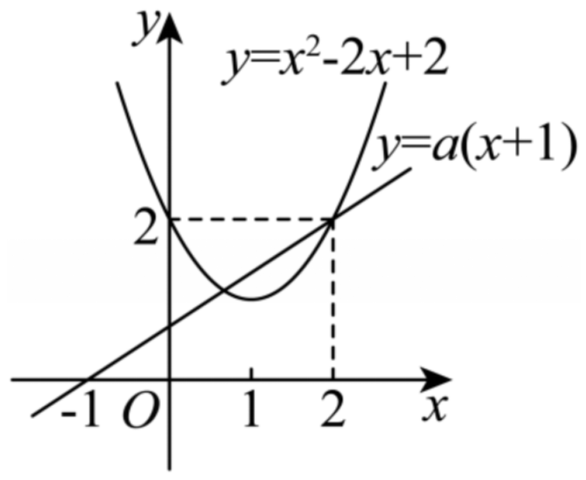
\includegraphics[width=0.30\textwidth]{figures/gao75_q12_graph.png}
\end{center}
% 原卷此处作“≥”，与题干严格不等号方向不一致，照录（见文件头“原卷笔误/存疑”①）
\step{由集合 $A$ 是“$2$ 集合”，故集合 $A$ 中只有一个元素，}
\step{得 $\begin{cases}2^2-2\times2+2\geqslant(2+1)a\\ 1^2-2\times1+2<(1+1)a\end{cases}$，解得 $\dfrac12<a\leqslant\dfrac23$，}
\step{故正实数 $a$ 的取值范围是 $\dfrac12<a\leqslant\dfrac23$.}
\solend
\fi

\end{enumerate}

\bigsec{二、选择题}

\begin{enumerate}
\setcounter{enumi}{12}

\item 已知全集 $U=\R$，集合 $A=\{x\mid x^2<4\}$，$B=\{y\mid y=x^2\}$，则图中阴影部分所表示的集合为\mbox{（\quad）}

\begin{center}
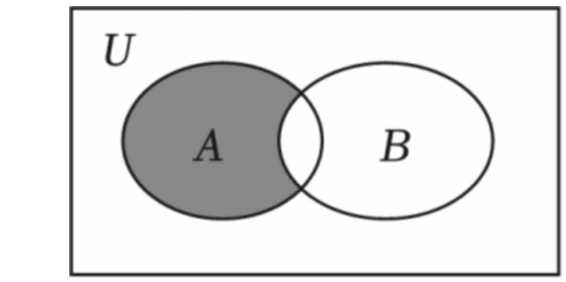
\includegraphics[width=0.26\textwidth]{figures/gao75_q13_venn.png}
\end{center}

\keepwithprev
A. $\{-2,-1,0\}$\qquad B. $(-\infty,4)$\qquad C. $(-2,0)$\qquad D. $(-2,0]$

\ifanswer
\solbegin
\step{集合 $A=\{x\mid x^2<4\}=(-2,2)$，$B=\{y\mid y=x^2\}=[0,+\infty)$，}
\step{图中阴影部分所表示的集合是 $A\cap\overline{B}=(-2,0)$. 故选 $C$.}
\solend
\fi

\item 已知 $x\in\R$，则“$\dfrac1x>1$”是“$x<1$”的\mbox{（\quad）}

\keepwithprev
A. 充分非必要条件\qquad B. 必要非充分条件\qquad C. 充要条件\qquad D. 既非充分又非必要条件

\ifanswer
\solbegin
\step{“$\dfrac1x>1$”$\Leftrightarrow0<x<1$，所以“$\dfrac1x>1$”是“$x<1$”的充分不必要条件. 故选 $A$.}
\solend
\fi

\item 已知集合 $M=\{x\mid x=m+\dfrac16,\,m\in\Z\}$，$N=\{x\mid x=\dfrac n2-\dfrac13,\,n\in\Z\}$，\\
$P=\{x\mid x=\dfrac p2+\dfrac16,\,p\in\Z\}$，则 $M$、$N$、$P$ 的关系为\mbox{（\quad）}

\keepwithprev
A. $M=N\subseteq P$\qquad B. $M\subseteq N=P$\qquad C. $M\subseteq N\subseteq P$\qquad D. $N\subseteq P\subseteq M$

\ifanswer
\solbegin
\step{集合 $N=\{x\mid x=\dfrac n2-\dfrac13,\,n\in\Z\}$，则 $x=\dfrac n2-\dfrac13=\dfrac{3n-2}6$，$n\in\Z$.}
\step{$P=\{x\mid x=\dfrac p2+\dfrac16,\,p\in\Z\}$，则 $x=\dfrac p2+\dfrac16=\dfrac{3p+1}6$，$p\in\Z$.}
\step{$M=\{x\mid x=m+\dfrac16,\,m\in\Z\}$，则 $x=m+\dfrac16=\dfrac{6m+1}6$，$m\in\Z$.}
\step{$M$、$N$、$P$ 三者分母相同，所以只需要比较他们的分子.}
\step{$M$：$6$ 的倍数$+1$，$N=P$：$3$ 的倍数$+1$，所以 $M\subseteq N=P$. 故选 $B$.}
\solend
\fi

\item 设集合 $P_1=\{x\mid x^2+ax+1>0\}$，$P_2=\{x\mid x^2+ax+2>0\}$，$Q_1=\{x\mid x^2+x+b>0\}$，$Q_2=\{x\mid x^2+2x+b>0\}$ 其中 $a,b\in\R$，给出下列两个命题：命题 $q_1$：对任意的 $a$，$P_1$ 是 $P_2$ 的子集；命题 $q_2$：对任意的 $b$，$Q_1$ 不是 $Q_2$ 的子集. 下列说法正确的是\mbox{（\quad）}

\keepwithprev
A. 命题 $q_1$ 是真命题，命题 $q_2$ 是假命题\qquad B. 命题 $q_1$ 是假命题，命题 $q_2$ 是真命题

C. 命题 $q_1$、$q_2$ 都是真命题\qquad D. 命题 $q_1$、$q_2$ 都是假命题

\ifanswer
\solbegin
\step{对于集合 $P_1=\{x\mid x^2+ax+1>0\}$，$P_2=\{x\mid x^2+ax+2>0\}$，}
\step{当 $m\in P_1$，即 $m^2+am+1>0$，得 $m^2+am+2>0$，}
\step{即有 $m\in P_2$，得对任意 $a$，$P_1$ 是 $P_2$ 的子集，命题 $q_1$ 为真命题；}
\step{当 $b=5$ 时，$Q_1=\{x\mid x^2+x+5>0\}=\R$，$Q_2=\{x\mid x^2+2x+5>0\}=\R$，}
\step{得 $Q_1$ 是 $Q_2$ 的子集；}
\step{存在 $b$，使得 $Q_1$ 是 $Q_2$ 的子集，故命题 $q_2$ 是假命题.}
\step{故选 $A$.}
\solend
\fi

\end{enumerate}

\bigsec{三、解答题}

\begin{enumerate}
\setcounter{enumi}{16}

\item 设集合 $A=\{x\mid x^2-2x=0\}$，$B=\{x\mid x^2+2(a+1)x+a^2-1=0\}$.

（1）写出集合 $A$ 的所有子集；

（2）若 $A\cap B=B$，求实数 $a$ 的取值范围.

\ifanswer
\solbegin
\stepm{(1)}{由 $x^2-2x=0$，得 $x=2$ 或 $x=0$，所以 $A=\{0,2\}$，}
\step{故集合 $A$ 的所有子集为 $\varnothing$、$\{0\}$、$\{2\}$、$\{0,2\}$.}
\stepm{(2)}{因为 $A\cap B=B$，所以 $B\subseteq A$，}
\step{方程 $x^2+2(a+1)x+a^2-1=0$，$\Delta=4(a+1)^2-4(a^2-1)=8a+8$，}
\step{若 $\Delta<0$，即 $a<-1$，方程 $x^2+2(a+1)x+a^2-1=0$ 无解，}
\step{此时 $B=\varnothing$，满足题意；}
\step{若 $\Delta=0$，即 $a=-1$，由 $x^2+2(a+1)x+a^2-1=0$，即 $x^2=0$，}
\step{解得 $x=0$，此时 $B=\{0\}$，满足题意；}
\step{若 $\Delta>0$，即 $a>-1$，要使 $B\subseteq A$，}
\step{则方程 $x^2+2(a+1)x+a^2-1=0$ 的解集为 $\{0,2\}$，}
\step{则 $\begin{cases}2+0=-2(a+1)\\ 2\times0=a^2-1\end{cases}$，$a$ 不存在.}
\step{综上所述，$a\leqslant-1$，即实数 $a$ 的取值范围为 $\{a\mid a\leqslant-1\}$.}
\solend
\fi

\ansspace

\item 已知全集 $U=\R$，集合 $A=\left\{x\,\middle|\,\dfrac{x-1}{x-3}<0\right\}$，$B=\{x\mid|x-a|<2\}$.

（1）当 $a=1$ 时，试用区间表示集合 $A$、$B$；

（2）若 $A\cup B=B$，求实数 $a$ 的取值范围.

\ifanswer
\solbegin
\stepm{(1)}{不等式 $\dfrac{x-1}{x-3}<0$ 可化为 $(x-1)(x-3)<0$，解得 $1<x<3$，即 $A=(1,3)$，}
\step{当 $a=1$ 时，$|x-1|<2$，则 $-2<x-1<2$，解得 $-1<x<3$，}
\step{即 $B=(-1,3)$；}
\stepm{(2)}{由不等式 $|x-a|<2$ 得 $-2<x-a<2$，解得 $-2+a<x<2+a$，}
\step{即 $B=\{x\mid-2+a<x<2+a\}$，}
\step{因为 $A\cup B=B$，所以 $A\subseteq B$，则 $\begin{cases}-2+a\leqslant1\\ 2+a\geqslant3\end{cases}$，解得 $1\leqslant a\leqslant3$，}
\step{即实数 $a$ 的取值范围为 $[1,3]$.}
\solend
\fi

\ansspace

\item 法国数学家弗朗索瓦·韦达 1615 年在著作《论方程的识别与订正》中建立了方程根与系数的关系. 发现一元二次方程 $ax^2+bx+c=0$，$a\neq0$ 的根与系数有如下的关系：

$x_1+x_2=-\dfrac ba$，$x_1x_2=\dfrac ca$，此即为韦达定理. 韦达定理的逆定理仍成立：如果两个数 $x_1$，$x_2$ 满足 $x_1+x_2=-\dfrac ba$，$x_1x_2=\dfrac ca$，则这两个数 $x_1$、$x_2$ 是方程 $ax^2+bx+c=0$，$a\neq0$ 的两个根. 例如：$m+n=-3$，$mn=2$，则 $m$、$n$ 是方程 $x^2+3x+2=0$ 的两个根. 请根据上述材料解决以下问题.

（1）已知 $m$、$n$ 是两个不相等的实数，满足 $m^2-6m-5=0$，$n^2-6n-5=0$，求 $\dfrac1m+\dfrac1n$ 的值；

（2）已知实数 $x$、$y$ 满足 $x+y+xy=17$，$x^2y+xy^2=72$，求 $x^2+y^2$ 的值.

\ifanswer
\solbegin
\stepm{(1)}{由题意，不相等的实数 $m$、$n$ 满足 $m^2-6m-5=0$、$n^2-6n-5=0$，}
\step{因此 $m$、$n$ 是一元二次方程 $x^2-6x-5=0$ 的两个不等实根.}
\step{由韦达定理得 $m+n=6$，$mn=-5$，因此 $\dfrac1m+\dfrac1n=\dfrac{m+n}{mn}=\dfrac6{-5}=-\dfrac65$.}
\stepm{(2)}{令 $s=x+y$，$t=xy$，}
\step{因为 $x+y+xy=17$，$x^2y+xy^2=72$，}
\step{即 $x+y+xy=17$，$xy(x+y)=72$，将已知条件变形得 $\begin{cases}s+t=17\\ st=72\end{cases}$.}
\step{由韦达定理逆定理，$s$、$t$ 是一元二次方程 $z^2-17z+72=0$ 的两个实根，}
\step{解方程得 $z_1=8$，$z_2=9$，即有两组解 $\begin{cases}s=8\\ t=9\end{cases}$ 和 $\begin{cases}s=9\\ t=8\end{cases}$.}
\step{当 $\begin{cases}s=8\\ t=9\end{cases}$ 时，$x$、$y$ 是方程 $w^2-8w+9=0$ 的根，}
\step{判别式 $\Delta=8^2-4\times1\times9=64-36=28>0$，符合题意，}
\step{此时 $x^2+y^2=(x+y)^2-2xy=s^2-2t=8^2-2\times9=64-18=46$；}
\step{当 $\begin{cases}s=9\\ t=8\end{cases}$ 时，$x$、$y$ 是方程 $w^2-9w+8=0$ 的根，}
\step{判别式 $\Delta=9^2-4\times1\times8=81-32=49>0$，符合题意，}
\step{此时 $x^2+y^2=(x+y)^2-2xy=s^2-2t=9^2-2\times8=81-16=65$.}
\step{综上，$x^2+y^2$ 的值为 $46$ 或 $65$.}
\solend
\fi

\ansspace

\item 已知关于 $x$ 的不等式 $ax^2-(a+1)x+b<0$.

（1）若不等式的解集是 $\{x\mid1<x<5\}$，求 $a+b$ 的值；

（2）若 $b=-\dfrac12$ 且不等式的解集为 $\R$，求 $a$ 取值范围；

（3）若 $b=1$，讨论此不等式的解集.

\ifanswer
\solbegin
\stepm{(1)}{由题意得 $1$ 和 $5$ 是方程 $ax^2-(a+1)x+b=0$ 的两个根且 $a>0$，}
\step{所以 $1+5=\dfrac{a+1}a$，$1\times5=\dfrac ba$，解得 $a=\dfrac15$，$b=1$，所以 $a+b=\dfrac65$.}
\stepm{(2)}{若 $b=-\dfrac12$，则不等式为 $ax^2-(a+1)x-\dfrac12<0$，}
\step{当 $a\neq0$，则有 $\begin{cases}a<0\\ \Delta=(a+1)^2+2a<0\end{cases}$，解得 $-2-\sqrt3<a<-2+\sqrt3$；}
\step{当 $a=0$，不等式即为 $-x-\dfrac12<0$，则 $x>-\dfrac12$，不合题意；}
\step{所以 $a$ 的取值范围是 $(-2-\sqrt3,-2+\sqrt3)$.}
\stepm{(3)}{若 $b=1$，则不等式为 $ax^2-(a+1)x+1<0$，即 $(ax-1)(x-1)<0$.}
\step{当 $a\neq0$ 时，由 $ax^2-(a+1)x+1<0$ 得 $(ax-1)(x-1)<0$.}
\step{方程 $(ax-1)(x-1)=0$ 的根为 $x=\dfrac1a$ 或 $x=1$，}
\step{当 $0<a<1$ 时，$\dfrac1a>1$，则不等式的解集为 $\left(1,\dfrac1a\right)$；}
\step{当 $a<0$ 时，$\dfrac1a<1$，则不等式的解集为 $\left(-\infty,\dfrac1a\right)\cup(1,+\infty)$；}
\step{当 $a=1$ 时，不等式即为 $(x-1)^2<0$，则不等式的解集为 $\varnothing$；}
\step{当 $a>1$ 时，$\dfrac1a<1$，则不等式的解集为 $\left(\dfrac1a,1\right)$；}
\step{当 $a=0$ 时，不等式为 $-x+1<0$，则不等式的解集为 $(1,+\infty)$；}
\step{综上所述，当 $a<0$ 时，不等式的解集为 $\left(-\infty,\dfrac1a\right)\cup(1,+\infty)$；}
\step{当 $a=0$ 时，不等式的解集为 $(1,+\infty)$；}
\step{当 $0<a<1$ 时，不等式的解集为 $\left(1,\dfrac1a\right)$；}
\step{当 $a=1$ 时，不等式的解集为 $\varnothing$；}
\step{当 $a>1$ 时，不等式的解集为 $\left(\dfrac1a,1\right)$.}
\solend
\fi

\ansspace

\item 已知关于 $x$ 的不等式① $x^2+2cx+c>0$，② $x^2+cx+c^2-1>0$，其中 $c$ 是实数.

（1）若 $1$ 是不等式②的一个解，求实数 $c$ 的取值范围；

（2）证明：不等式①、②中至多有一个恒成立；

（3）当 $c=0$ 时，“$x$ 满足 $|mx^2-4x+3|>5$”的一个必要非充分条件是“$x$ 满足 $x^2+cx+c^2-1>0$，求实数 $m$ 的取值范围.

\ifanswer
\solbegin
\stepm{(1)}{因为 $1$ 是不等式②的一个解，所以 $1+c+c^2-1>0$，}
\step{即 $c(c+1)>0$，解得 $c>0$ 或 $c<-1$，}
\step{所以实数 $c$ 的取值范围为 $(-\infty,-1)\cup(0,+\infty)$.}
\stepm{(2)}{假设不等式①、②都恒成立，}
\step{不等式① $x^2+2cx+c>0$ 恒成立，所以 $4c^2-4c<0$，所以 $0<c<1$；}
\step{② $x^2+cx+c^2-1>0$ 恒成立，所以 $c^2-4(c^2-1)<0$，$c^2>\dfrac43$，}
\step{解得 $c>\dfrac{2\sqrt3}3$ 或 $c<-\dfrac{2\sqrt3}3$；}
\step{所以当不等式①、②都恒成立时，}
\step{不等式组 $\begin{cases}0<c<1\\ c\in\left(-\infty,-\dfrac{2\sqrt3}3\right)\cup\left(\dfrac{2\sqrt3}3,+\infty\right)\end{cases}$ 无解，}
\step{所以假设不成立，}
\step{所以不等式①、②中至多有一个恒成立.}
\stepm{(3)}{当 $c=0$ 时，由 $x^2+cx+c^2-1>0$ 得 $x^2-1>0$，}
\step{解集为 $(-\infty,-1)\cup(1,+\infty)$.}
\step{记集合 $A=\{x\mid|mx^2-4x+3|>5\}$，集合 $B=\{x\mid x<-1\text{ 或 }x>1\}$.}
\step{由“$x$ 满足 $|mx^2-4x+3|>5$”的一个必要非充分条件是}
\step{“$x$ 满足 $x^2+cx+c^2-1>0$”得 $A$ 是 $B$ 的真子集.}
\step{所以 $\overline{B}$ 是 $A$ 的真子集，即对任意 $x\in[-1,1]$，$|mx^2-4x+3|\leqslant5$ 恒成立.}
\step{当 $x=0$ 时，不等式 $-5\leqslant mx^2-4x+3\leqslant5$ 恒成立；}
\step{当 $x\in[-1,0)\cup(0,1]$ 时，}
\step{则 $mx^2-4x+3\geqslant-5$ 与 $mx^2-4x+3\leqslant5$ 同时成立.}
\step{①由 $mx^2-4x+3\geqslant-5$，得 $m\geqslant\dfrac{4x-8}{x^2}$，求值域得 $\dfrac{4x-8}{x^2}$ 的最大值 $=-4$，}
\step{所以 $m\geqslant-4$.}
\step{②由 $mx^2-4x+3\leqslant5$，得 $m\leqslant\dfrac{4x+2}{x^2}$，求值域得 $\dfrac{4x+2}{x^2}$ 的最小值 $=-2$，}
\step{所以 $m\leqslant-2$.}
\step{综上所述，实数 $m$ 的取值范围为 $[-4,-2]$.}
\solend
\fi

\ansspace*[7]

\end{enumerate}

\end{document}
"
%
% 原始材料：微信公众号“魔都数学加油站”文章，连载“27学年高一75”；
% 原文标题“27学年高一75——2026-2027年上海市市二中学高一上10月月考”；
% 原文链接：https://mp.weixin.qq.com/s/dhxtwWEZgKLxeKdkbWqOhw。
% 页面标注发布时间 2026-10-22 21:45（上海）。
% 正文为 11 张 PNG 页（`原图/高一75_市二中学_10月月考/01..11.png`）：
% 第 2、4、5、6、9 页为 4762×6735，其余 6 页为 2560×3620，均按页序读取。
% 11 页全为试卷正文页（卷首标题在第 1 页页顶，卷末第 21 题 (3) 解析止于第 11 页），
% 无封面页、目录页、二维码或宣传页。粉色斜排“魔都数学加油站”为卷面水印，未录入。
%
% 卷首标题：照卷面印作“2026-2027 年市二中学高一上 10 月月考”（黑体加粗一行）。
% 原卷年份区间用半角连字符，本稿按全稿惯例排 en dash；原卷无副标题。
%
% 篇幅与题号：原卷自第 3 题起编号（第 1、2 题不在本卷内）。填空题 3—12（10 题）、
% 选择题 13—16（4 题）、解答题 17—21（5 题），共 19 题。本稿沿用原节与原题号，
% 只改排为全稿统一的大节样式。
%
% 讲评版：原卷第 4 题只印【答案】（“$[-1,2]$”），本稿只给 \ans{}；其余 18 题均印
% 【解析】，用 \solbegin…\solend。四道选择题的作答括号原卷即留空，答案写在解析末句
% “故选 C／A／B／A”，照录在解析内，不另提 \ans{}。
%
% 副标题：原卷未印副标题。本稿按“知识模块”口径标作“集合与常用逻辑用语、不等式”：
% 19 题中集合与常用逻辑用语 9 题（第 3、4、5、8、10、12、13、15、17、18 题中的集合题），
% 不等式 10 题（第 6、7、9、11、19、20、21 题及第 12、20 题的不等式部分），两类均确有
% 分量，故并标。口径同 高一63、高一68—74。
%
% 与原卷的排版差异：
%   ① 原卷每题下直接印【答案】/【解析】，本稿按全稿惯例将答案与解析置于答案版；
%   ② 原卷未印副标题，本稿按“知识模块”口径补出；
%   ③ 原卷填空横线约四个字宽，本稿按全稿惯例统一排 \blankline[4.4em]；
%   ④ 原卷数集记号排粗体 $\mathbf{R}$（第 5、6、7、9、10、14、18、20、21 题），本稿
%      按全稿惯例改用 $\R$（同 高一68—74）；第 11 题的“解集为 $\R$”同此；
%   ⑤ 原卷句末标点多为西文句点，均逐处照录；
%   ⑥ 第 17—21 题的子问原卷印作“（1）…（2）…”，本稿按 高一69—74 成例用行内
%      “（1）（2）（3）”段，解析中的子问标号用 \stepm{(1)}{…}；
%   ⑦ 每道解答题原卷未留作答空白，本稿按全稿惯例加 \ansspace（末题用 \ansspace*）；
%   ⑧ 选择题的作答括号原卷排半角“(    )”，本稿按全稿惯例排 \mbox{（\quad）}；
%      选项行排照原卷——第 13、14 题一行四条，第 15、16 题一行四条；
%   ⑨ 第 9、12、15、17—21 题解析中的不等式组／方程组，原卷均排作“{”连接的多行式，
%      本稿按全稿惯例排 cases；
%   ⑩ 第 12 题解析有一幅“抛物线 + 直线”图：原卷印在解析第 3 行右侧、题干无“如图”二字
%      （解析里写“两函数图象如图：”）。本稿按原卷截图裁取（`figures/gao75_q12_graph.png`，
%      由第 3 页原图裁出、去除粉色水印后转灰度，未放大），放在答案版解析第 3 条之后；
%   ⑪ 第 13 题题干中间有一幅韦恩图（全集矩形内含 A、B 两圆，A 涂灰）：原卷印在题干
%      右侧、题干句子被图隔开。本稿按原卷截图裁取（`figures/gao75_q13_venn.png`，由第 3
%      页原图裁出、去除粉色水印后转灰度，并抹去左侧侵入的“分”字），放在题干之后、
%      选项之前，仅答案版出。
%
% 原卷笔误/存疑（均照录未改，正文对应处另有 % 注）：
%   ① 第 12 题解析列不等式组时写 $2^2-2\times2+2\geqslant(2+1)a$，与
%      $x^2-2x+2<a(x+1)$ 的严格不等号方向不一致；原卷如此，照录未改。
%   ② 第 14 题选项 A—D 的“充分非必要”“必要非充分”“既非充分又非必要”与原卷
%      其它题的“充分不必要”写法不同，照录未统一。
%   ④ 第 21 题 (3) 题干的“$x$ 满足 $|mx^2-4x+3|>5$”的一个必要非充分条件是
%      “$x$ 满足 $x^2+cx+c^2-1>0$，原卷只有左引号、无右引号（且逗号在引号内），
%      本稿照录未补。
%   ③ 第 20 题 (2) 的解集写成 $(-2-\sqrt3,-2+\sqrt3)$，其中 $a<0$ 与 $\Delta<0$ 联立后
%      左端点应为 $-2-\sqrt3$、右端点为 $-2+\sqrt3$；原卷如此，照录未改。
%
% 行数核对：逐题数 \step/\stepm 条数与原卷【解析】印刷行数，18 题逐一相符，
% 合计 132 条 / 132 行（Q3：6；Q5：1；Q6：2；Q7：1；Q8：2；Q9：3；Q10：10；
% Q11：8；Q12：6；Q13：2；Q14：1；Q15：5；Q16：7；Q17：12；Q18：7；Q19：15；
% Q20：19；Q21：25）。另第 4 题只印【答案】，提 \ans{}，不计入 \step 账。
%
% 插图：第 12 题解析的抛物线图、第 13 题题干的韦恩图，见上⑩⑪；其余题干无配图。
%
\documentclass[a4paper,11pt]{article}
\usepackage{common}

\begin{document}

\examtitlest[3]{2026--2027 年市二中学高一上 10 月月考}{集合与常用逻辑用语、不等式}

\bigsec{一、填空题}

\begin{enumerate}
\setcounter{enumi}{2}

\item 已知集合 $A=\{a,a^2\}$，且 $1\in A$，则 $a=$\blankline[4.4em].

\ifanswer
\solbegin
\step{因为 $1\in A=\{a,a^2\}$，所以 $a=1$ 或 $a^2=1$.}
\step{又集合 $A=\{a,a^2\}$ 是用列举法写出两个元素的，其元素必须互异，故 $a\neq a^2$，}
\step{即 $a\neq0$ 且 $a\neq1$，所以 $a=1$ 应舍去；}
\step{由 $a^2=1$ 得 $a=1$（舍去）或 $a=-1$.}
\step{当 $a=-1$ 时，$A=\{-1,1\}$，满足 $1\in A$ 且两个元素互异.}
\step{故 $a=-1$.}
\solend
\fi

\item 已知集合 $A=[-1,1]$，$B=[0,2]$，则 $A\cup B=$\blankline[4.4em].

\ifanswer
\ans{$[-1,2]$}
\fi

\item 已知全集 $U=\R$，集合 $A=\{x\mid x\neq1\}$，则 $\overline{A}=$\blankline[4.4em].

\ifanswer
\solbegin
\step{因为全集 $U=\R$，集合 $A=\{x\mid x\neq1\}$，所以 $\overline{A}=\{x\mid x=1\}$.}
\solend
\fi

\item 设 $x\in\R$，不等式 $x^2-4x<0$ 的解集用区间表示是\blankline[4.4em].

\ifanswer
\solbegin
\step{因为 $x^2-4x<0$，即 $x(x-4)<0$，所以 $0<x<4$，}
\step{所以 $x(x-4)<0$ 的解集为 $(0,4)$.}
\solend
\fi

\item 已知 $m\in\R$，若关于 $x$ 的方程 $2mx^2+3x+m-1=m^2\cdot x^2+(m+1)x+1$ 解集为 $\R$，则 $m$ 的值为\blankline[4.4em].

\ifanswer
\solbegin
\step{由题意得 $2m=m^2$，$3=m+1$，$m-1=1$，所以 $m=2$.}
\solend
\fi

\item 设 $\alpha:x\leqslant m$，$\beta:|x-2|\leqslant1$，若 $\alpha$ 是 $\beta$ 的必要条件，则实数 $m$ 的取值范围是\blankline[4.4em].

\ifanswer
\solbegin
\step{由 $|x-2|\leqslant1$，得 $-1\leqslant x-2\leqslant1$，解得 $1\leqslant x\leqslant3$，}
\step{因为 $\alpha$ 是 $\beta$ 的必要条件，所以 $\{x\mid1\leqslant x\leqslant3\}\subseteq\{x\mid x\leqslant m\}$，得 $m\geqslant3$.}
\solend
\fi

\item 设 $a\in\R$，若关于 $x$ 的不等式 $\dfrac{a}{x-1}\leqslant1$ 的解集是 $(-\infty,1)\cup[2,+\infty)$，则 $a$ 的值为\blankline[4.4em].

\ifanswer
\solbegin
\step{不等式可变形为 $\dfrac{a+1-x}{x-1}\leqslant0$，等价于 $\begin{cases}(a+1-x)(x-1)\leqslant0\\ x-1\neq0\end{cases}$，}
\step{因为原不等式的解集是 $(-\infty,1)\cup[2,+\infty)$，}
\step{所以 $1$，$2$ 是方程 $(a+1-x)(x-1)=0$ 的两根，所以 $a+1=2$，解得 $a=1$.}
\solend
\fi

\item 下列命题：① “$x>1$ 或 $y>1$”的否定形式是“$x\leqslant1$ 或 $y\leqslant1$”，② 若 $A\cup B=B$，则 $A\subseteq B$，③ 方程 $ax+1=0$ 的解是 $x=-\frac1a$，④ “$ac=bc$”是“$a=b$”的必要非充分条件，⑤ “任意 $x\in\R$，$f(x)=f(-x)$”的否定形式是“存在 $x_0\in\R$，使得 $f(x_0)\neq f(-x_0)$”其中真命题的序号是\blankline[4.4em]（填写序号）.

\ifanswer
\solbegin
\step{①假命题：“$x>1$ 或 $y>1$”的否定形式是“$x\leqslant1$ 且 $y\leqslant1$”；}
\step{②真命题：$A\cup B=B\Leftrightarrow A\subseteq B$；}
\step{③假命题：当 $a=0$ 时，方程无解，因此该命题忽略了 $a=0$ 的情况；}
\step{④真命题：先判断必要性：若 $a=b$，则有 $ac=bc$，所以必要性成立；}
\step{再判断充分性：若 $ac=bc$，即 $(a-b)c=0$，当 $c=0$ 时，$a$ 和 $b$ 可以不相等，}
\step{因此充分性不成立.}
\step{⑤真命题：全称命题的否定是存在量词命题，}
\step{“任意 $x\in\R$，$f(x)=f(-x)$”的否定形式是}
\step{“存在 $x_0\in\R$，使得 $f(x_0)\neq f(-x_0)$”，表述正确.}
\step{故正确的是②④⑤.}
\solend
\fi

\item 为了加强家校联系，蔡老师组建了一个由学生、家长和教师组成的微信群. 已知该群中男学生人数多于女学生人数，女学生人数多于家长人数，家长人数多于教师人数，教师人数的两倍多于男学生人数. 则该微信群人数的最小值为\blankline[4.4em].

\ifanswer
\solbegin
\step{设男学生、女学生、家长、教师的人数分别为 $M$、$F$、$P$、$T$，}
\step{它们都是正整数.}
\step{由题意得 $M>F>P>T$，且教师人数的两倍多于男学生人数，即 $2T>M$.}
\step{由 $M>F>P>T$ 得 $M\geqslant T+3$；}
\step{又 $2T>M\geqslant T+3$，所以 $2T>T+3$，解得 $T>3$，故教师人数最少为 $T=4$.}
\step{当 $T=4$ 时，为使总人数最少，取 $P=5$、$F=6$、$M=7$，}
\step{此时 $7>6>5>4$ 且 $2\times4=8>7$，满足题意.}
\step{于是微信群人数为 $4+5+6+7=22$，所以该微信群人数的最小值为 $22$.}
\solend
\fi

\item 若集合 $M$ 有 $k$ 个子集，则称集合 $M$ 为“$k$ 集合”，\\
已知集合 $A=\{x\mid x^2-(a+2)x+2-a<0,\,x\in\Z\}$ 是“$2$ 集合”，则正实数 $a$ 的取值范围是\blankline[4.4em].

\ifanswer
\solbegin
\step{由 $x^2-(a+2)x+2-a<0$，得 $x^2-2x+2<a(x+1)$，}
\step{设二次函数 $y=x^2-2x+2$ 与一次函数 $y=a(x+1)$，}
\needvspace{13\baselineskip}
\step{由 $a>0$，$y=a(x+1)$ 过定点 $(-1,0)$，两函数图象如图：}
\begin{center}
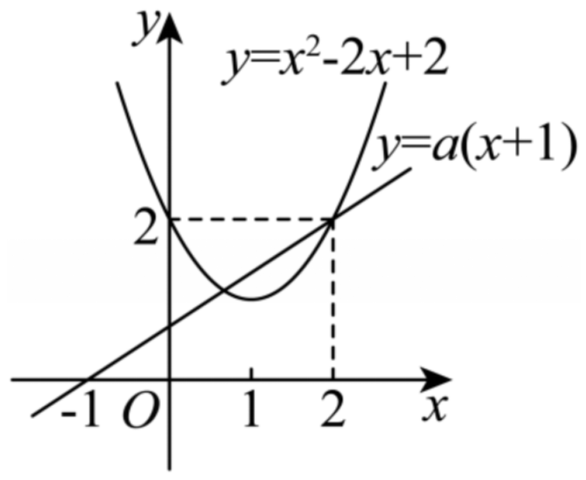
\includegraphics[width=0.30\textwidth]{figures/gao75_q12_graph.png}
\end{center}
% 原卷此处作“≥”，与题干严格不等号方向不一致，照录（见文件头“原卷笔误/存疑”①）
\step{由集合 $A$ 是“$2$ 集合”，故集合 $A$ 中只有一个元素，}
\step{得 $\begin{cases}2^2-2\times2+2\geqslant(2+1)a\\ 1^2-2\times1+2<(1+1)a\end{cases}$，解得 $\dfrac12<a\leqslant\dfrac23$，}
\step{故正实数 $a$ 的取值范围是 $\dfrac12<a\leqslant\dfrac23$.}
\solend
\fi

\end{enumerate}

\bigsec{二、选择题}

\begin{enumerate}
\setcounter{enumi}{12}

\item 已知全集 $U=\R$，集合 $A=\{x\mid x^2<4\}$，$B=\{y\mid y=x^2\}$，则图中阴影部分所表示的集合为\mbox{（\quad）}

\begin{center}
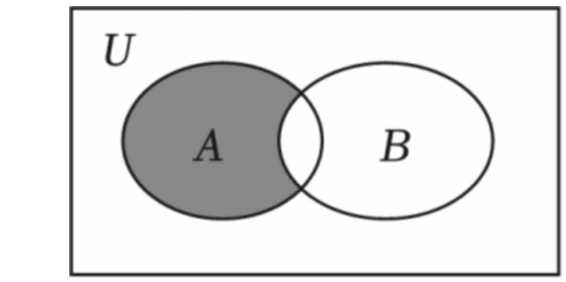
\includegraphics[width=0.26\textwidth]{figures/gao75_q13_venn.png}
\end{center}

\keepwithprev
A. $\{-2,-1,0\}$\qquad B. $(-\infty,4)$\qquad C. $(-2,0)$\qquad D. $(-2,0]$

\ifanswer
\solbegin
\step{集合 $A=\{x\mid x^2<4\}=(-2,2)$，$B=\{y\mid y=x^2\}=[0,+\infty)$，}
\step{图中阴影部分所表示的集合是 $A\cap\overline{B}=(-2,0)$. 故选 $C$.}
\solend
\fi

\item 已知 $x\in\R$，则“$\dfrac1x>1$”是“$x<1$”的\mbox{（\quad）}

\keepwithprev
A. 充分非必要条件\qquad B. 必要非充分条件\qquad C. 充要条件\qquad D. 既非充分又非必要条件

\ifanswer
\solbegin
\step{“$\dfrac1x>1$”$\Leftrightarrow0<x<1$，所以“$\dfrac1x>1$”是“$x<1$”的充分不必要条件. 故选 $A$.}
\solend
\fi

\item 已知集合 $M=\{x\mid x=m+\dfrac16,\,m\in\Z\}$，$N=\{x\mid x=\dfrac n2-\dfrac13,\,n\in\Z\}$，\\
$P=\{x\mid x=\dfrac p2+\dfrac16,\,p\in\Z\}$，则 $M$、$N$、$P$ 的关系为\mbox{（\quad）}

\keepwithprev
A. $M=N\subseteq P$\qquad B. $M\subseteq N=P$\qquad C. $M\subseteq N\subseteq P$\qquad D. $N\subseteq P\subseteq M$

\ifanswer
\solbegin
\step{集合 $N=\{x\mid x=\dfrac n2-\dfrac13,\,n\in\Z\}$，则 $x=\dfrac n2-\dfrac13=\dfrac{3n-2}6$，$n\in\Z$.}
\step{$P=\{x\mid x=\dfrac p2+\dfrac16,\,p\in\Z\}$，则 $x=\dfrac p2+\dfrac16=\dfrac{3p+1}6$，$p\in\Z$.}
\step{$M=\{x\mid x=m+\dfrac16,\,m\in\Z\}$，则 $x=m+\dfrac16=\dfrac{6m+1}6$，$m\in\Z$.}
\step{$M$、$N$、$P$ 三者分母相同，所以只需要比较他们的分子.}
\step{$M$：$6$ 的倍数$+1$，$N=P$：$3$ 的倍数$+1$，所以 $M\subseteq N=P$. 故选 $B$.}
\solend
\fi

\item 设集合 $P_1=\{x\mid x^2+ax+1>0\}$，$P_2=\{x\mid x^2+ax+2>0\}$，$Q_1=\{x\mid x^2+x+b>0\}$，$Q_2=\{x\mid x^2+2x+b>0\}$ 其中 $a,b\in\R$，给出下列两个命题：命题 $q_1$：对任意的 $a$，$P_1$ 是 $P_2$ 的子集；命题 $q_2$：对任意的 $b$，$Q_1$ 不是 $Q_2$ 的子集. 下列说法正确的是\mbox{（\quad）}

\keepwithprev
A. 命题 $q_1$ 是真命题，命题 $q_2$ 是假命题\qquad B. 命题 $q_1$ 是假命题，命题 $q_2$ 是真命题

C. 命题 $q_1$、$q_2$ 都是真命题\qquad D. 命题 $q_1$、$q_2$ 都是假命题

\ifanswer
\solbegin
\step{对于集合 $P_1=\{x\mid x^2+ax+1>0\}$，$P_2=\{x\mid x^2+ax+2>0\}$，}
\step{当 $m\in P_1$，即 $m^2+am+1>0$，得 $m^2+am+2>0$，}
\step{即有 $m\in P_2$，得对任意 $a$，$P_1$ 是 $P_2$ 的子集，命题 $q_1$ 为真命题；}
\step{当 $b=5$ 时，$Q_1=\{x\mid x^2+x+5>0\}=\R$，$Q_2=\{x\mid x^2+2x+5>0\}=\R$，}
\step{得 $Q_1$ 是 $Q_2$ 的子集；}
\step{存在 $b$，使得 $Q_1$ 是 $Q_2$ 的子集，故命题 $q_2$ 是假命题.}
\step{故选 $A$.}
\solend
\fi

\end{enumerate}

\bigsec{三、解答题}

\begin{enumerate}
\setcounter{enumi}{16}

\item 设集合 $A=\{x\mid x^2-2x=0\}$，$B=\{x\mid x^2+2(a+1)x+a^2-1=0\}$.

（1）写出集合 $A$ 的所有子集；

（2）若 $A\cap B=B$，求实数 $a$ 的取值范围.

\ifanswer
\solbegin
\stepm{(1)}{由 $x^2-2x=0$，得 $x=2$ 或 $x=0$，所以 $A=\{0,2\}$，}
\step{故集合 $A$ 的所有子集为 $\varnothing$、$\{0\}$、$\{2\}$、$\{0,2\}$.}
\stepm{(2)}{因为 $A\cap B=B$，所以 $B\subseteq A$，}
\step{方程 $x^2+2(a+1)x+a^2-1=0$，$\Delta=4(a+1)^2-4(a^2-1)=8a+8$，}
\step{若 $\Delta<0$，即 $a<-1$，方程 $x^2+2(a+1)x+a^2-1=0$ 无解，}
\step{此时 $B=\varnothing$，满足题意；}
\step{若 $\Delta=0$，即 $a=-1$，由 $x^2+2(a+1)x+a^2-1=0$，即 $x^2=0$，}
\step{解得 $x=0$，此时 $B=\{0\}$，满足题意；}
\step{若 $\Delta>0$，即 $a>-1$，要使 $B\subseteq A$，}
\step{则方程 $x^2+2(a+1)x+a^2-1=0$ 的解集为 $\{0,2\}$，}
\step{则 $\begin{cases}2+0=-2(a+1)\\ 2\times0=a^2-1\end{cases}$，$a$ 不存在.}
\step{综上所述，$a\leqslant-1$，即实数 $a$ 的取值范围为 $\{a\mid a\leqslant-1\}$.}
\solend
\fi

\ansspace

\item 已知全集 $U=\R$，集合 $A=\left\{x\,\middle|\,\dfrac{x-1}{x-3}<0\right\}$，$B=\{x\mid|x-a|<2\}$.

（1）当 $a=1$ 时，试用区间表示集合 $A$、$B$；

（2）若 $A\cup B=B$，求实数 $a$ 的取值范围.

\ifanswer
\solbegin
\stepm{(1)}{不等式 $\dfrac{x-1}{x-3}<0$ 可化为 $(x-1)(x-3)<0$，解得 $1<x<3$，即 $A=(1,3)$，}
\step{当 $a=1$ 时，$|x-1|<2$，则 $-2<x-1<2$，解得 $-1<x<3$，}
\step{即 $B=(-1,3)$；}
\stepm{(2)}{由不等式 $|x-a|<2$ 得 $-2<x-a<2$，解得 $-2+a<x<2+a$，}
\step{即 $B=\{x\mid-2+a<x<2+a\}$，}
\step{因为 $A\cup B=B$，所以 $A\subseteq B$，则 $\begin{cases}-2+a\leqslant1\\ 2+a\geqslant3\end{cases}$，解得 $1\leqslant a\leqslant3$，}
\step{即实数 $a$ 的取值范围为 $[1,3]$.}
\solend
\fi

\ansspace

\item 法国数学家弗朗索瓦·韦达 1615 年在著作《论方程的识别与订正》中建立了方程根与系数的关系. 发现一元二次方程 $ax^2+bx+c=0$，$a\neq0$ 的根与系数有如下的关系：

$x_1+x_2=-\dfrac ba$，$x_1x_2=\dfrac ca$，此即为韦达定理. 韦达定理的逆定理仍成立：如果两个数 $x_1$，$x_2$ 满足 $x_1+x_2=-\dfrac ba$，$x_1x_2=\dfrac ca$，则这两个数 $x_1$、$x_2$ 是方程 $ax^2+bx+c=0$，$a\neq0$ 的两个根. 例如：$m+n=-3$，$mn=2$，则 $m$、$n$ 是方程 $x^2+3x+2=0$ 的两个根. 请根据上述材料解决以下问题.

（1）已知 $m$、$n$ 是两个不相等的实数，满足 $m^2-6m-5=0$，$n^2-6n-5=0$，求 $\dfrac1m+\dfrac1n$ 的值；

（2）已知实数 $x$、$y$ 满足 $x+y+xy=17$，$x^2y+xy^2=72$，求 $x^2+y^2$ 的值.

\ifanswer
\solbegin
\stepm{(1)}{由题意，不相等的实数 $m$、$n$ 满足 $m^2-6m-5=0$、$n^2-6n-5=0$，}
\step{因此 $m$、$n$ 是一元二次方程 $x^2-6x-5=0$ 的两个不等实根.}
\step{由韦达定理得 $m+n=6$，$mn=-5$，因此 $\dfrac1m+\dfrac1n=\dfrac{m+n}{mn}=\dfrac6{-5}=-\dfrac65$.}
\stepm{(2)}{令 $s=x+y$，$t=xy$，}
\step{因为 $x+y+xy=17$，$x^2y+xy^2=72$，}
\step{即 $x+y+xy=17$，$xy(x+y)=72$，将已知条件变形得 $\begin{cases}s+t=17\\ st=72\end{cases}$.}
\step{由韦达定理逆定理，$s$、$t$ 是一元二次方程 $z^2-17z+72=0$ 的两个实根，}
\step{解方程得 $z_1=8$，$z_2=9$，即有两组解 $\begin{cases}s=8\\ t=9\end{cases}$ 和 $\begin{cases}s=9\\ t=8\end{cases}$.}
\step{当 $\begin{cases}s=8\\ t=9\end{cases}$ 时，$x$、$y$ 是方程 $w^2-8w+9=0$ 的根，}
\step{判别式 $\Delta=8^2-4\times1\times9=64-36=28>0$，符合题意，}
\step{此时 $x^2+y^2=(x+y)^2-2xy=s^2-2t=8^2-2\times9=64-18=46$；}
\step{当 $\begin{cases}s=9\\ t=8\end{cases}$ 时，$x$、$y$ 是方程 $w^2-9w+8=0$ 的根，}
\step{判别式 $\Delta=9^2-4\times1\times8=81-32=49>0$，符合题意，}
\step{此时 $x^2+y^2=(x+y)^2-2xy=s^2-2t=9^2-2\times8=81-16=65$.}
\step{综上，$x^2+y^2$ 的值为 $46$ 或 $65$.}
\solend
\fi

\ansspace

\item 已知关于 $x$ 的不等式 $ax^2-(a+1)x+b<0$.

（1）若不等式的解集是 $\{x\mid1<x<5\}$，求 $a+b$ 的值；

（2）若 $b=-\dfrac12$ 且不等式的解集为 $\R$，求 $a$ 取值范围；

（3）若 $b=1$，讨论此不等式的解集.

\ifanswer
\solbegin
\stepm{(1)}{由题意得 $1$ 和 $5$ 是方程 $ax^2-(a+1)x+b=0$ 的两个根且 $a>0$，}
\step{所以 $1+5=\dfrac{a+1}a$，$1\times5=\dfrac ba$，解得 $a=\dfrac15$，$b=1$，所以 $a+b=\dfrac65$.}
\stepm{(2)}{若 $b=-\dfrac12$，则不等式为 $ax^2-(a+1)x-\dfrac12<0$，}
\step{当 $a\neq0$，则有 $\begin{cases}a<0\\ \Delta=(a+1)^2+2a<0\end{cases}$，解得 $-2-\sqrt3<a<-2+\sqrt3$；}
\step{当 $a=0$，不等式即为 $-x-\dfrac12<0$，则 $x>-\dfrac12$，不合题意；}
\step{所以 $a$ 的取值范围是 $(-2-\sqrt3,-2+\sqrt3)$.}
\stepm{(3)}{若 $b=1$，则不等式为 $ax^2-(a+1)x+1<0$，即 $(ax-1)(x-1)<0$.}
\step{当 $a\neq0$ 时，由 $ax^2-(a+1)x+1<0$ 得 $(ax-1)(x-1)<0$.}
\step{方程 $(ax-1)(x-1)=0$ 的根为 $x=\dfrac1a$ 或 $x=1$，}
\step{当 $0<a<1$ 时，$\dfrac1a>1$，则不等式的解集为 $\left(1,\dfrac1a\right)$；}
\step{当 $a<0$ 时，$\dfrac1a<1$，则不等式的解集为 $\left(-\infty,\dfrac1a\right)\cup(1,+\infty)$；}
\step{当 $a=1$ 时，不等式即为 $(x-1)^2<0$，则不等式的解集为 $\varnothing$；}
\step{当 $a>1$ 时，$\dfrac1a<1$，则不等式的解集为 $\left(\dfrac1a,1\right)$；}
\step{当 $a=0$ 时，不等式为 $-x+1<0$，则不等式的解集为 $(1,+\infty)$；}
\step{综上所述，当 $a<0$ 时，不等式的解集为 $\left(-\infty,\dfrac1a\right)\cup(1,+\infty)$；}
\step{当 $a=0$ 时，不等式的解集为 $(1,+\infty)$；}
\step{当 $0<a<1$ 时，不等式的解集为 $\left(1,\dfrac1a\right)$；}
\step{当 $a=1$ 时，不等式的解集为 $\varnothing$；}
\step{当 $a>1$ 时，不等式的解集为 $\left(\dfrac1a,1\right)$.}
\solend
\fi

\ansspace

\item 已知关于 $x$ 的不等式① $x^2+2cx+c>0$，② $x^2+cx+c^2-1>0$，其中 $c$ 是实数.

（1）若 $1$ 是不等式②的一个解，求实数 $c$ 的取值范围；

（2）证明：不等式①、②中至多有一个恒成立；

（3）当 $c=0$ 时，“$x$ 满足 $|mx^2-4x+3|>5$”的一个必要非充分条件是“$x$ 满足 $x^2+cx+c^2-1>0$，求实数 $m$ 的取值范围.

\ifanswer
\solbegin
\stepm{(1)}{因为 $1$ 是不等式②的一个解，所以 $1+c+c^2-1>0$，}
\step{即 $c(c+1)>0$，解得 $c>0$ 或 $c<-1$，}
\step{所以实数 $c$ 的取值范围为 $(-\infty,-1)\cup(0,+\infty)$.}
\stepm{(2)}{假设不等式①、②都恒成立，}
\step{不等式① $x^2+2cx+c>0$ 恒成立，所以 $4c^2-4c<0$，所以 $0<c<1$；}
\step{② $x^2+cx+c^2-1>0$ 恒成立，所以 $c^2-4(c^2-1)<0$，$c^2>\dfrac43$，}
\step{解得 $c>\dfrac{2\sqrt3}3$ 或 $c<-\dfrac{2\sqrt3}3$；}
\step{所以当不等式①、②都恒成立时，}
\step{不等式组 $\begin{cases}0<c<1\\ c\in\left(-\infty,-\dfrac{2\sqrt3}3\right)\cup\left(\dfrac{2\sqrt3}3,+\infty\right)\end{cases}$ 无解，}
\step{所以假设不成立，}
\step{所以不等式①、②中至多有一个恒成立.}
\stepm{(3)}{当 $c=0$ 时，由 $x^2+cx+c^2-1>0$ 得 $x^2-1>0$，}
\step{解集为 $(-\infty,-1)\cup(1,+\infty)$.}
\step{记集合 $A=\{x\mid|mx^2-4x+3|>5\}$，集合 $B=\{x\mid x<-1\text{ 或 }x>1\}$.}
\step{由“$x$ 满足 $|mx^2-4x+3|>5$”的一个必要非充分条件是}
\step{“$x$ 满足 $x^2+cx+c^2-1>0$”得 $A$ 是 $B$ 的真子集.}
\step{所以 $\overline{B}$ 是 $A$ 的真子集，即对任意 $x\in[-1,1]$，$|mx^2-4x+3|\leqslant5$ 恒成立.}
\step{当 $x=0$ 时，不等式 $-5\leqslant mx^2-4x+3\leqslant5$ 恒成立；}
\step{当 $x\in[-1,0)\cup(0,1]$ 时，}
\step{则 $mx^2-4x+3\geqslant-5$ 与 $mx^2-4x+3\leqslant5$ 同时成立.}
\step{①由 $mx^2-4x+3\geqslant-5$，得 $m\geqslant\dfrac{4x-8}{x^2}$，求值域得 $\dfrac{4x-8}{x^2}$ 的最大值 $=-4$，}
\step{所以 $m\geqslant-4$.}
\step{②由 $mx^2-4x+3\leqslant5$，得 $m\leqslant\dfrac{4x+2}{x^2}$，求值域得 $\dfrac{4x+2}{x^2}$ 的最小值 $=-2$，}
\step{所以 $m\leqslant-2$.}
\step{综上所述，实数 $m$ 的取值范围为 $[-4,-2]$.}
\solend
\fi

\ansspace*[7]

\end{enumerate}

\end{document}
"
%
% 原始材料：微信公众号“魔都数学加油站”文章，连载“27学年高一75”；
% 原文标题“27学年高一75——2026-2027年上海市市二中学高一上10月月考”；
% 原文链接：https://mp.weixin.qq.com/s/dhxtwWEZgKLxeKdkbWqOhw。
% 页面标注发布时间 2026-10-22 21:45（上海）。
% 正文为 11 张 PNG 页（`原图/高一75_市二中学_10月月考/01..11.png`）：
% 第 2、4、5、6、9 页为 4762×6735，其余 6 页为 2560×3620，均按页序读取。
% 11 页全为试卷正文页（卷首标题在第 1 页页顶，卷末第 21 题 (3) 解析止于第 11 页），
% 无封面页、目录页、二维码或宣传页。粉色斜排“魔都数学加油站”为卷面水印，未录入。
%
% 卷首标题：照卷面印作“2026-2027 年市二中学高一上 10 月月考”（黑体加粗一行）。
% 原卷年份区间用半角连字符，本稿按全稿惯例排 en dash；原卷无副标题。
%
% 篇幅与题号：原卷自第 3 题起编号（第 1、2 题不在本卷内）。填空题 3—12（10 题）、
% 选择题 13—16（4 题）、解答题 17—21（5 题），共 19 题。本稿沿用原节与原题号，
% 只改排为全稿统一的大节样式。
%
% 讲评版：原卷第 4 题只印【答案】（“$[-1,2]$”），本稿只给 \ans{}；其余 18 题均印
% 【解析】，用 \solbegin…\solend。四道选择题的作答括号原卷即留空，答案写在解析末句
% “故选 C／A／B／A”，照录在解析内，不另提 \ans{}。
%
% 副标题：原卷未印副标题。本稿按“知识模块”口径标作“集合与常用逻辑用语、不等式”：
% 19 题中集合与常用逻辑用语 9 题（第 3、4、5、8、10、12、13、15、17、18 题中的集合题），
% 不等式 10 题（第 6、7、9、11、19、20、21 题及第 12、20 题的不等式部分），两类均确有
% 分量，故并标。口径同 高一63、高一68—74。
%
% 与原卷的排版差异：
%   ① 原卷每题下直接印【答案】/【解析】，本稿按全稿惯例将答案与解析置于答案版；
%   ② 原卷未印副标题，本稿按“知识模块”口径补出；
%   ③ 原卷填空横线约四个字宽，本稿按全稿惯例统一排 \blankline[4.4em]；
%   ④ 原卷数集记号排粗体 $\mathbf{R}$（第 5、6、7、9、10、14、18、20、21 题），本稿
%      按全稿惯例改用 $\R$（同 高一68—74）；第 11 题的“解集为 $\R$”同此；
%   ⑤ 原卷句末标点多为西文句点，均逐处照录；
%   ⑥ 第 17—21 题的子问原卷印作“（1）…（2）…”，本稿按 高一69—74 成例用行内
%      “（1）（2）（3）”段，解析中的子问标号用 \stepm{(1)}{…}；
%   ⑦ 每道解答题原卷未留作答空白，本稿按全稿惯例加 \ansspace（末题用 \ansspace*）；
%   ⑧ 选择题的作答括号原卷排半角“(    )”，本稿按全稿惯例排 \mbox{（\quad）}；
%      选项行排照原卷——第 13、14 题一行四条，第 15、16 题一行四条；
%   ⑨ 第 9、12、15、17—21 题解析中的不等式组／方程组，原卷均排作“{”连接的多行式，
%      本稿按全稿惯例排 cases；
%   ⑩ 第 12 题解析有一幅“抛物线 + 直线”图：原卷印在解析第 3 行右侧、题干无“如图”二字
%      （解析里写“两函数图象如图：”）。本稿按原卷截图裁取（`figures/gao75_q12_graph.png`，
%      由第 3 页原图裁出、去除粉色水印后转灰度，未放大），放在答案版解析第 3 条之后；
%   ⑪ 第 13 题题干中间有一幅韦恩图（全集矩形内含 A、B 两圆，A 涂灰）：原卷印在题干
%      右侧、题干句子被图隔开。本稿按原卷截图裁取（`figures/gao75_q13_venn.png`，由第 3
%      页原图裁出、去除粉色水印后转灰度，并抹去左侧侵入的“分”字），放在题干之后、
%      选项之前，仅答案版出。
%
% 原卷笔误/存疑（均照录未改，正文对应处另有 % 注）：
%   ① 第 12 题解析列不等式组时写 $2^2-2\times2+2\geqslant(2+1)a$，与
%      $x^2-2x+2<a(x+1)$ 的严格不等号方向不一致；原卷如此，照录未改。
%   ② 第 14 题选项 A—D 的“充分非必要”“必要非充分”“既非充分又非必要”与原卷
%      其它题的“充分不必要”写法不同，照录未统一。
%   ④ 第 21 题 (3) 题干的“$x$ 满足 $|mx^2-4x+3|>5$”的一个必要非充分条件是
%      “$x$ 满足 $x^2+cx+c^2-1>0$，原卷只有左引号、无右引号（且逗号在引号内），
%      本稿照录未补。
%   ③ 第 20 题 (2) 的解集写成 $(-2-\sqrt3,-2+\sqrt3)$，其中 $a<0$ 与 $\Delta<0$ 联立后
%      左端点应为 $-2-\sqrt3$、右端点为 $-2+\sqrt3$；原卷如此，照录未改。
%
% 行数核对：逐题数 \step/\stepm 条数与原卷【解析】印刷行数，18 题逐一相符，
% 合计 132 条 / 132 行（Q3：6；Q5：1；Q6：2；Q7：1；Q8：2；Q9：3；Q10：10；
% Q11：8；Q12：6；Q13：2；Q14：1；Q15：5；Q16：7；Q17：12；Q18：7；Q19：15；
% Q20：19；Q21：25）。另第 4 题只印【答案】，提 \ans{}，不计入 \step 账。
%
% 插图：第 12 题解析的抛物线图、第 13 题题干的韦恩图，见上⑩⑪；其余题干无配图。
%
\documentclass[a4paper,11pt]{article}
\usepackage{common}

\begin{document}

\examtitlest[3]{2026--2027 年市二中学高一上 10 月月考}{集合与常用逻辑用语、不等式}

\bigsec{一、填空题}

\begin{enumerate}
\setcounter{enumi}{2}

\item 已知集合 $A=\{a,a^2\}$，且 $1\in A$，则 $a=$\blankline[4.4em].

\ifanswer
\solbegin
\step{因为 $1\in A=\{a,a^2\}$，所以 $a=1$ 或 $a^2=1$.}
\step{又集合 $A=\{a,a^2\}$ 是用列举法写出两个元素的，其元素必须互异，故 $a\neq a^2$，}
\step{即 $a\neq0$ 且 $a\neq1$，所以 $a=1$ 应舍去；}
\step{由 $a^2=1$ 得 $a=1$（舍去）或 $a=-1$.}
\step{当 $a=-1$ 时，$A=\{-1,1\}$，满足 $1\in A$ 且两个元素互异.}
\step{故 $a=-1$.}
\solend
\fi

\item 已知集合 $A=[-1,1]$，$B=[0,2]$，则 $A\cup B=$\blankline[4.4em].

\ifanswer
\ans{$[-1,2]$}
\fi

\item 已知全集 $U=\R$，集合 $A=\{x\mid x\neq1\}$，则 $\overline{A}=$\blankline[4.4em].

\ifanswer
\solbegin
\step{因为全集 $U=\R$，集合 $A=\{x\mid x\neq1\}$，所以 $\overline{A}=\{x\mid x=1\}$.}
\solend
\fi

\item 设 $x\in\R$，不等式 $x^2-4x<0$ 的解集用区间表示是\blankline[4.4em].

\ifanswer
\solbegin
\step{因为 $x^2-4x<0$，即 $x(x-4)<0$，所以 $0<x<4$，}
\step{所以 $x(x-4)<0$ 的解集为 $(0,4)$.}
\solend
\fi

\item 已知 $m\in\R$，若关于 $x$ 的方程 $2mx^2+3x+m-1=m^2\cdot x^2+(m+1)x+1$ 解集为 $\R$，则 $m$ 的值为\blankline[4.4em].

\ifanswer
\solbegin
\step{由题意得 $2m=m^2$，$3=m+1$，$m-1=1$，所以 $m=2$.}
\solend
\fi

\item 设 $\alpha:x\leqslant m$，$\beta:|x-2|\leqslant1$，若 $\alpha$ 是 $\beta$ 的必要条件，则实数 $m$ 的取值范围是\blankline[4.4em].

\ifanswer
\solbegin
\step{由 $|x-2|\leqslant1$，得 $-1\leqslant x-2\leqslant1$，解得 $1\leqslant x\leqslant3$，}
\step{因为 $\alpha$ 是 $\beta$ 的必要条件，所以 $\{x\mid1\leqslant x\leqslant3\}\subseteq\{x\mid x\leqslant m\}$，得 $m\geqslant3$.}
\solend
\fi

\item 设 $a\in\R$，若关于 $x$ 的不等式 $\dfrac{a}{x-1}\leqslant1$ 的解集是 $(-\infty,1)\cup[2,+\infty)$，则 $a$ 的值为\blankline[4.4em].

\ifanswer
\solbegin
\step{不等式可变形为 $\dfrac{a+1-x}{x-1}\leqslant0$，等价于 $\begin{cases}(a+1-x)(x-1)\leqslant0\\ x-1\neq0\end{cases}$，}
\step{因为原不等式的解集是 $(-\infty,1)\cup[2,+\infty)$，}
\step{所以 $1$，$2$ 是方程 $(a+1-x)(x-1)=0$ 的两根，所以 $a+1=2$，解得 $a=1$.}
\solend
\fi

\item 下列命题：① “$x>1$ 或 $y>1$”的否定形式是“$x\leqslant1$ 或 $y\leqslant1$”，② 若 $A\cup B=B$，则 $A\subseteq B$，③ 方程 $ax+1=0$ 的解是 $x=-\frac1a$，④ “$ac=bc$”是“$a=b$”的必要非充分条件，⑤ “任意 $x\in\R$，$f(x)=f(-x)$”的否定形式是“存在 $x_0\in\R$，使得 $f(x_0)\neq f(-x_0)$”其中真命题的序号是\blankline[4.4em]（填写序号）.

\ifanswer
\solbegin
\step{①假命题：“$x>1$ 或 $y>1$”的否定形式是“$x\leqslant1$ 且 $y\leqslant1$”；}
\step{②真命题：$A\cup B=B\Leftrightarrow A\subseteq B$；}
\step{③假命题：当 $a=0$ 时，方程无解，因此该命题忽略了 $a=0$ 的情况；}
\step{④真命题：先判断必要性：若 $a=b$，则有 $ac=bc$，所以必要性成立；}
\step{再判断充分性：若 $ac=bc$，即 $(a-b)c=0$，当 $c=0$ 时，$a$ 和 $b$ 可以不相等，}
\step{因此充分性不成立.}
\step{⑤真命题：全称命题的否定是存在量词命题，}
\step{“任意 $x\in\R$，$f(x)=f(-x)$”的否定形式是}
\step{“存在 $x_0\in\R$，使得 $f(x_0)\neq f(-x_0)$”，表述正确.}
\step{故正确的是②④⑤.}
\solend
\fi

\item 为了加强家校联系，蔡老师组建了一个由学生、家长和教师组成的微信群. 已知该群中男学生人数多于女学生人数，女学生人数多于家长人数，家长人数多于教师人数，教师人数的两倍多于男学生人数. 则该微信群人数的最小值为\blankline[4.4em].

\ifanswer
\solbegin
\step{设男学生、女学生、家长、教师的人数分别为 $M$、$F$、$P$、$T$，}
\step{它们都是正整数.}
\step{由题意得 $M>F>P>T$，且教师人数的两倍多于男学生人数，即 $2T>M$.}
\step{由 $M>F>P>T$ 得 $M\geqslant T+3$；}
\step{又 $2T>M\geqslant T+3$，所以 $2T>T+3$，解得 $T>3$，故教师人数最少为 $T=4$.}
\step{当 $T=4$ 时，为使总人数最少，取 $P=5$、$F=6$、$M=7$，}
\step{此时 $7>6>5>4$ 且 $2\times4=8>7$，满足题意.}
\step{于是微信群人数为 $4+5+6+7=22$，所以该微信群人数的最小值为 $22$.}
\solend
\fi

\item 若集合 $M$ 有 $k$ 个子集，则称集合 $M$ 为“$k$ 集合”，\\
已知集合 $A=\{x\mid x^2-(a+2)x+2-a<0,\,x\in\Z\}$ 是“$2$ 集合”，则正实数 $a$ 的取值范围是\blankline[4.4em].

\ifanswer
\solbegin
\step{由 $x^2-(a+2)x+2-a<0$，得 $x^2-2x+2<a(x+1)$，}
\step{设二次函数 $y=x^2-2x+2$ 与一次函数 $y=a(x+1)$，}
\needvspace{13\baselineskip}
\step{由 $a>0$，$y=a(x+1)$ 过定点 $(-1,0)$，两函数图象如图：}
\begin{center}
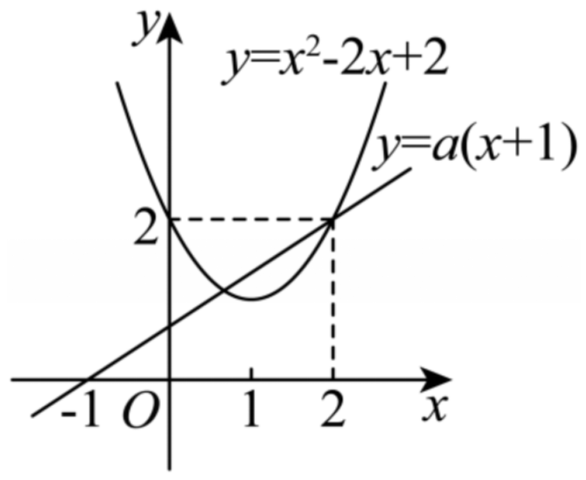
\includegraphics[width=0.30\textwidth]{figures/gao75_q12_graph.png}
\end{center}
% 原卷此处作“≥”，与题干严格不等号方向不一致，照录（见文件头“原卷笔误/存疑”①）
\step{由集合 $A$ 是“$2$ 集合”，故集合 $A$ 中只有一个元素，}
\step{得 $\begin{cases}2^2-2\times2+2\geqslant(2+1)a\\ 1^2-2\times1+2<(1+1)a\end{cases}$，解得 $\dfrac12<a\leqslant\dfrac23$，}
\step{故正实数 $a$ 的取值范围是 $\dfrac12<a\leqslant\dfrac23$.}
\solend
\fi

\end{enumerate}

\bigsec{二、选择题}

\begin{enumerate}
\setcounter{enumi}{12}

\item 已知全集 $U=\R$，集合 $A=\{x\mid x^2<4\}$，$B=\{y\mid y=x^2\}$，则图中阴影部分所表示的集合为\mbox{（\quad）}

\begin{center}
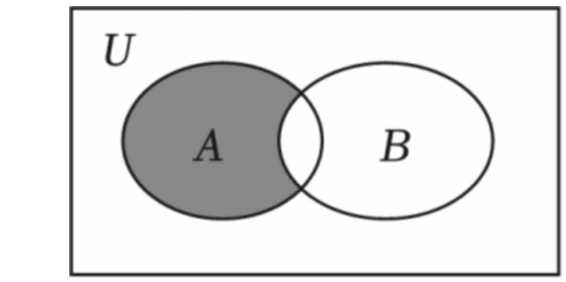
\includegraphics[width=0.26\textwidth]{figures/gao75_q13_venn.png}
\end{center}

\keepwithprev
A. $\{-2,-1,0\}$\qquad B. $(-\infty,4)$\qquad C. $(-2,0)$\qquad D. $(-2,0]$

\ifanswer
\solbegin
\step{集合 $A=\{x\mid x^2<4\}=(-2,2)$，$B=\{y\mid y=x^2\}=[0,+\infty)$，}
\step{图中阴影部分所表示的集合是 $A\cap\overline{B}=(-2,0)$. 故选 $C$.}
\solend
\fi

\item 已知 $x\in\R$，则“$\dfrac1x>1$”是“$x<1$”的\mbox{（\quad）}

\keepwithprev
A. 充分非必要条件\qquad B. 必要非充分条件\qquad C. 充要条件\qquad D. 既非充分又非必要条件

\ifanswer
\solbegin
\step{“$\dfrac1x>1$”$\Leftrightarrow0<x<1$，所以“$\dfrac1x>1$”是“$x<1$”的充分不必要条件. 故选 $A$.}
\solend
\fi

\item 已知集合 $M=\{x\mid x=m+\dfrac16,\,m\in\Z\}$，$N=\{x\mid x=\dfrac n2-\dfrac13,\,n\in\Z\}$，\\
$P=\{x\mid x=\dfrac p2+\dfrac16,\,p\in\Z\}$，则 $M$、$N$、$P$ 的关系为\mbox{（\quad）}

\keepwithprev
A. $M=N\subseteq P$\qquad B. $M\subseteq N=P$\qquad C. $M\subseteq N\subseteq P$\qquad D. $N\subseteq P\subseteq M$

\ifanswer
\solbegin
\step{集合 $N=\{x\mid x=\dfrac n2-\dfrac13,\,n\in\Z\}$，则 $x=\dfrac n2-\dfrac13=\dfrac{3n-2}6$，$n\in\Z$.}
\step{$P=\{x\mid x=\dfrac p2+\dfrac16,\,p\in\Z\}$，则 $x=\dfrac p2+\dfrac16=\dfrac{3p+1}6$，$p\in\Z$.}
\step{$M=\{x\mid x=m+\dfrac16,\,m\in\Z\}$，则 $x=m+\dfrac16=\dfrac{6m+1}6$，$m\in\Z$.}
\step{$M$、$N$、$P$ 三者分母相同，所以只需要比较他们的分子.}
\step{$M$：$6$ 的倍数$+1$，$N=P$：$3$ 的倍数$+1$，所以 $M\subseteq N=P$. 故选 $B$.}
\solend
\fi

\item 设集合 $P_1=\{x\mid x^2+ax+1>0\}$，$P_2=\{x\mid x^2+ax+2>0\}$，$Q_1=\{x\mid x^2+x+b>0\}$，$Q_2=\{x\mid x^2+2x+b>0\}$ 其中 $a,b\in\R$，给出下列两个命题：命题 $q_1$：对任意的 $a$，$P_1$ 是 $P_2$ 的子集；命题 $q_2$：对任意的 $b$，$Q_1$ 不是 $Q_2$ 的子集. 下列说法正确的是\mbox{（\quad）}

\keepwithprev
A. 命题 $q_1$ 是真命题，命题 $q_2$ 是假命题\qquad B. 命题 $q_1$ 是假命题，命题 $q_2$ 是真命题

C. 命题 $q_1$、$q_2$ 都是真命题\qquad D. 命题 $q_1$、$q_2$ 都是假命题

\ifanswer
\solbegin
\step{对于集合 $P_1=\{x\mid x^2+ax+1>0\}$，$P_2=\{x\mid x^2+ax+2>0\}$，}
\step{当 $m\in P_1$，即 $m^2+am+1>0$，得 $m^2+am+2>0$，}
\step{即有 $m\in P_2$，得对任意 $a$，$P_1$ 是 $P_2$ 的子集，命题 $q_1$ 为真命题；}
\step{当 $b=5$ 时，$Q_1=\{x\mid x^2+x+5>0\}=\R$，$Q_2=\{x\mid x^2+2x+5>0\}=\R$，}
\step{得 $Q_1$ 是 $Q_2$ 的子集；}
\step{存在 $b$，使得 $Q_1$ 是 $Q_2$ 的子集，故命题 $q_2$ 是假命题.}
\step{故选 $A$.}
\solend
\fi

\end{enumerate}

\bigsec{三、解答题}

\begin{enumerate}
\setcounter{enumi}{16}

\item 设集合 $A=\{x\mid x^2-2x=0\}$，$B=\{x\mid x^2+2(a+1)x+a^2-1=0\}$.

（1）写出集合 $A$ 的所有子集；

（2）若 $A\cap B=B$，求实数 $a$ 的取值范围.

\ifanswer
\solbegin
\stepm{(1)}{由 $x^2-2x=0$，得 $x=2$ 或 $x=0$，所以 $A=\{0,2\}$，}
\step{故集合 $A$ 的所有子集为 $\varnothing$、$\{0\}$、$\{2\}$、$\{0,2\}$.}
\stepm{(2)}{因为 $A\cap B=B$，所以 $B\subseteq A$，}
\step{方程 $x^2+2(a+1)x+a^2-1=0$，$\Delta=4(a+1)^2-4(a^2-1)=8a+8$，}
\step{若 $\Delta<0$，即 $a<-1$，方程 $x^2+2(a+1)x+a^2-1=0$ 无解，}
\step{此时 $B=\varnothing$，满足题意；}
\step{若 $\Delta=0$，即 $a=-1$，由 $x^2+2(a+1)x+a^2-1=0$，即 $x^2=0$，}
\step{解得 $x=0$，此时 $B=\{0\}$，满足题意；}
\step{若 $\Delta>0$，即 $a>-1$，要使 $B\subseteq A$，}
\step{则方程 $x^2+2(a+1)x+a^2-1=0$ 的解集为 $\{0,2\}$，}
\step{则 $\begin{cases}2+0=-2(a+1)\\ 2\times0=a^2-1\end{cases}$，$a$ 不存在.}
\step{综上所述，$a\leqslant-1$，即实数 $a$ 的取值范围为 $\{a\mid a\leqslant-1\}$.}
\solend
\fi

\ansspace

\item 已知全集 $U=\R$，集合 $A=\left\{x\,\middle|\,\dfrac{x-1}{x-3}<0\right\}$，$B=\{x\mid|x-a|<2\}$.

（1）当 $a=1$ 时，试用区间表示集合 $A$、$B$；

（2）若 $A\cup B=B$，求实数 $a$ 的取值范围.

\ifanswer
\solbegin
\stepm{(1)}{不等式 $\dfrac{x-1}{x-3}<0$ 可化为 $(x-1)(x-3)<0$，解得 $1<x<3$，即 $A=(1,3)$，}
\step{当 $a=1$ 时，$|x-1|<2$，则 $-2<x-1<2$，解得 $-1<x<3$，}
\step{即 $B=(-1,3)$；}
\stepm{(2)}{由不等式 $|x-a|<2$ 得 $-2<x-a<2$，解得 $-2+a<x<2+a$，}
\step{即 $B=\{x\mid-2+a<x<2+a\}$，}
\step{因为 $A\cup B=B$，所以 $A\subseteq B$，则 $\begin{cases}-2+a\leqslant1\\ 2+a\geqslant3\end{cases}$，解得 $1\leqslant a\leqslant3$，}
\step{即实数 $a$ 的取值范围为 $[1,3]$.}
\solend
\fi

\ansspace

\item 法国数学家弗朗索瓦·韦达 1615 年在著作《论方程的识别与订正》中建立了方程根与系数的关系. 发现一元二次方程 $ax^2+bx+c=0$，$a\neq0$ 的根与系数有如下的关系：

$x_1+x_2=-\dfrac ba$，$x_1x_2=\dfrac ca$，此即为韦达定理. 韦达定理的逆定理仍成立：如果两个数 $x_1$，$x_2$ 满足 $x_1+x_2=-\dfrac ba$，$x_1x_2=\dfrac ca$，则这两个数 $x_1$、$x_2$ 是方程 $ax^2+bx+c=0$，$a\neq0$ 的两个根. 例如：$m+n=-3$，$mn=2$，则 $m$、$n$ 是方程 $x^2+3x+2=0$ 的两个根. 请根据上述材料解决以下问题.

（1）已知 $m$、$n$ 是两个不相等的实数，满足 $m^2-6m-5=0$，$n^2-6n-5=0$，求 $\dfrac1m+\dfrac1n$ 的值；

（2）已知实数 $x$、$y$ 满足 $x+y+xy=17$，$x^2y+xy^2=72$，求 $x^2+y^2$ 的值.

\ifanswer
\solbegin
\stepm{(1)}{由题意，不相等的实数 $m$、$n$ 满足 $m^2-6m-5=0$、$n^2-6n-5=0$，}
\step{因此 $m$、$n$ 是一元二次方程 $x^2-6x-5=0$ 的两个不等实根.}
\step{由韦达定理得 $m+n=6$，$mn=-5$，因此 $\dfrac1m+\dfrac1n=\dfrac{m+n}{mn}=\dfrac6{-5}=-\dfrac65$.}
\stepm{(2)}{令 $s=x+y$，$t=xy$，}
\step{因为 $x+y+xy=17$，$x^2y+xy^2=72$，}
\step{即 $x+y+xy=17$，$xy(x+y)=72$，将已知条件变形得 $\begin{cases}s+t=17\\ st=72\end{cases}$.}
\step{由韦达定理逆定理，$s$、$t$ 是一元二次方程 $z^2-17z+72=0$ 的两个实根，}
\step{解方程得 $z_1=8$，$z_2=9$，即有两组解 $\begin{cases}s=8\\ t=9\end{cases}$ 和 $\begin{cases}s=9\\ t=8\end{cases}$.}
\step{当 $\begin{cases}s=8\\ t=9\end{cases}$ 时，$x$、$y$ 是方程 $w^2-8w+9=0$ 的根，}
\step{判别式 $\Delta=8^2-4\times1\times9=64-36=28>0$，符合题意，}
\step{此时 $x^2+y^2=(x+y)^2-2xy=s^2-2t=8^2-2\times9=64-18=46$；}
\step{当 $\begin{cases}s=9\\ t=8\end{cases}$ 时，$x$、$y$ 是方程 $w^2-9w+8=0$ 的根，}
\step{判别式 $\Delta=9^2-4\times1\times8=81-32=49>0$，符合题意，}
\step{此时 $x^2+y^2=(x+y)^2-2xy=s^2-2t=9^2-2\times8=81-16=65$.}
\step{综上，$x^2+y^2$ 的值为 $46$ 或 $65$.}
\solend
\fi

\ansspace

\item 已知关于 $x$ 的不等式 $ax^2-(a+1)x+b<0$.

（1）若不等式的解集是 $\{x\mid1<x<5\}$，求 $a+b$ 的值；

（2）若 $b=-\dfrac12$ 且不等式的解集为 $\R$，求 $a$ 取值范围；

（3）若 $b=1$，讨论此不等式的解集.

\ifanswer
\solbegin
\stepm{(1)}{由题意得 $1$ 和 $5$ 是方程 $ax^2-(a+1)x+b=0$ 的两个根且 $a>0$，}
\step{所以 $1+5=\dfrac{a+1}a$，$1\times5=\dfrac ba$，解得 $a=\dfrac15$，$b=1$，所以 $a+b=\dfrac65$.}
\stepm{(2)}{若 $b=-\dfrac12$，则不等式为 $ax^2-(a+1)x-\dfrac12<0$，}
\step{当 $a\neq0$，则有 $\begin{cases}a<0\\ \Delta=(a+1)^2+2a<0\end{cases}$，解得 $-2-\sqrt3<a<-2+\sqrt3$；}
\step{当 $a=0$，不等式即为 $-x-\dfrac12<0$，则 $x>-\dfrac12$，不合题意；}
\step{所以 $a$ 的取值范围是 $(-2-\sqrt3,-2+\sqrt3)$.}
\stepm{(3)}{若 $b=1$，则不等式为 $ax^2-(a+1)x+1<0$，即 $(ax-1)(x-1)<0$.}
\step{当 $a\neq0$ 时，由 $ax^2-(a+1)x+1<0$ 得 $(ax-1)(x-1)<0$.}
\step{方程 $(ax-1)(x-1)=0$ 的根为 $x=\dfrac1a$ 或 $x=1$，}
\step{当 $0<a<1$ 时，$\dfrac1a>1$，则不等式的解集为 $\left(1,\dfrac1a\right)$；}
\step{当 $a<0$ 时，$\dfrac1a<1$，则不等式的解集为 $\left(-\infty,\dfrac1a\right)\cup(1,+\infty)$；}
\step{当 $a=1$ 时，不等式即为 $(x-1)^2<0$，则不等式的解集为 $\varnothing$；}
\step{当 $a>1$ 时，$\dfrac1a<1$，则不等式的解集为 $\left(\dfrac1a,1\right)$；}
\step{当 $a=0$ 时，不等式为 $-x+1<0$，则不等式的解集为 $(1,+\infty)$；}
\step{综上所述，当 $a<0$ 时，不等式的解集为 $\left(-\infty,\dfrac1a\right)\cup(1,+\infty)$；}
\step{当 $a=0$ 时，不等式的解集为 $(1,+\infty)$；}
\step{当 $0<a<1$ 时，不等式的解集为 $\left(1,\dfrac1a\right)$；}
\step{当 $a=1$ 时，不等式的解集为 $\varnothing$；}
\step{当 $a>1$ 时，不等式的解集为 $\left(\dfrac1a,1\right)$.}
\solend
\fi

\ansspace

\item 已知关于 $x$ 的不等式① $x^2+2cx+c>0$，② $x^2+cx+c^2-1>0$，其中 $c$ 是实数.

（1）若 $1$ 是不等式②的一个解，求实数 $c$ 的取值范围；

（2）证明：不等式①、②中至多有一个恒成立；

（3）当 $c=0$ 时，“$x$ 满足 $|mx^2-4x+3|>5$”的一个必要非充分条件是“$x$ 满足 $x^2+cx+c^2-1>0$，求实数 $m$ 的取值范围.

\ifanswer
\solbegin
\stepm{(1)}{因为 $1$ 是不等式②的一个解，所以 $1+c+c^2-1>0$，}
\step{即 $c(c+1)>0$，解得 $c>0$ 或 $c<-1$，}
\step{所以实数 $c$ 的取值范围为 $(-\infty,-1)\cup(0,+\infty)$.}
\stepm{(2)}{假设不等式①、②都恒成立，}
\step{不等式① $x^2+2cx+c>0$ 恒成立，所以 $4c^2-4c<0$，所以 $0<c<1$；}
\step{② $x^2+cx+c^2-1>0$ 恒成立，所以 $c^2-4(c^2-1)<0$，$c^2>\dfrac43$，}
\step{解得 $c>\dfrac{2\sqrt3}3$ 或 $c<-\dfrac{2\sqrt3}3$；}
\step{所以当不等式①、②都恒成立时，}
\step{不等式组 $\begin{cases}0<c<1\\ c\in\left(-\infty,-\dfrac{2\sqrt3}3\right)\cup\left(\dfrac{2\sqrt3}3,+\infty\right)\end{cases}$ 无解，}
\step{所以假设不成立，}
\step{所以不等式①、②中至多有一个恒成立.}
\stepm{(3)}{当 $c=0$ 时，由 $x^2+cx+c^2-1>0$ 得 $x^2-1>0$，}
\step{解集为 $(-\infty,-1)\cup(1,+\infty)$.}
\step{记集合 $A=\{x\mid|mx^2-4x+3|>5\}$，集合 $B=\{x\mid x<-1\text{ 或 }x>1\}$.}
\step{由“$x$ 满足 $|mx^2-4x+3|>5$”的一个必要非充分条件是}
\step{“$x$ 满足 $x^2+cx+c^2-1>0$”得 $A$ 是 $B$ 的真子集.}
\step{所以 $\overline{B}$ 是 $A$ 的真子集，即对任意 $x\in[-1,1]$，$|mx^2-4x+3|\leqslant5$ 恒成立.}
\step{当 $x=0$ 时，不等式 $-5\leqslant mx^2-4x+3\leqslant5$ 恒成立；}
\step{当 $x\in[-1,0)\cup(0,1]$ 时，}
\step{则 $mx^2-4x+3\geqslant-5$ 与 $mx^2-4x+3\leqslant5$ 同时成立.}
\step{①由 $mx^2-4x+3\geqslant-5$，得 $m\geqslant\dfrac{4x-8}{x^2}$，求值域得 $\dfrac{4x-8}{x^2}$ 的最大值 $=-4$，}
\step{所以 $m\geqslant-4$.}
\step{②由 $mx^2-4x+3\leqslant5$，得 $m\leqslant\dfrac{4x+2}{x^2}$，求值域得 $\dfrac{4x+2}{x^2}$ 的最小值 $=-2$，}
\step{所以 $m\leqslant-2$.}
\step{综上所述，实数 $m$ 的取值范围为 $[-4,-2]$.}
\solend
\fi

\ansspace*[7]

\end{enumerate}

\end{document}
"
% 紧凑版：xelatex "\def\iscompact{1}% 高一75_市二中学_10月月考.tex
%   —— 高一上数学“2026-2027 年市二中学高一上 10 月月考”（讲评版）
% 试卷版：xelatex 高一75_市二中学_10月月考.tex
% 答案版：xelatex "\def\isanswer{1}% 高一75_市二中学_10月月考.tex
%   —— 高一上数学“2026-2027 年市二中学高一上 10 月月考”（讲评版）
% 试卷版：xelatex 高一75_市二中学_10月月考.tex
% 答案版：xelatex "\def\isanswer{1}% 高一75_市二中学_10月月考.tex
%   —— 高一上数学“2026-2027 年市二中学高一上 10 月月考”（讲评版）
% 试卷版：xelatex 高一75_市二中学_10月月考.tex
% 答案版：xelatex "\def\isanswer{1}\input{高一75_市二中学_10月月考.tex}"
% 紧凑版：xelatex "\def\iscompact{1}\input{高一75_市二中学_10月月考.tex}"
%
% 原始材料：微信公众号“魔都数学加油站”文章，连载“27学年高一75”；
% 原文标题“27学年高一75——2026-2027年上海市市二中学高一上10月月考”；
% 原文链接：https://mp.weixin.qq.com/s/dhxtwWEZgKLxeKdkbWqOhw。
% 页面标注发布时间 2026-10-22 21:45（上海）。
% 正文为 11 张 PNG 页（`原图/高一75_市二中学_10月月考/01..11.png`）：
% 第 2、4、5、6、9 页为 4762×6735，其余 6 页为 2560×3620，均按页序读取。
% 11 页全为试卷正文页（卷首标题在第 1 页页顶，卷末第 21 题 (3) 解析止于第 11 页），
% 无封面页、目录页、二维码或宣传页。粉色斜排“魔都数学加油站”为卷面水印，未录入。
%
% 卷首标题：照卷面印作“2026-2027 年市二中学高一上 10 月月考”（黑体加粗一行）。
% 原卷年份区间用半角连字符，本稿按全稿惯例排 en dash；原卷无副标题。
%
% 篇幅与题号：原卷自第 3 题起编号（第 1、2 题不在本卷内）。填空题 3—12（10 题）、
% 选择题 13—16（4 题）、解答题 17—21（5 题），共 19 题。本稿沿用原节与原题号，
% 只改排为全稿统一的大节样式。
%
% 讲评版：原卷第 4 题只印【答案】（“$[-1,2]$”），本稿只给 \ans{}；其余 18 题均印
% 【解析】，用 \solbegin…\solend。四道选择题的作答括号原卷即留空，答案写在解析末句
% “故选 C／A／B／A”，照录在解析内，不另提 \ans{}。
%
% 副标题：原卷未印副标题。本稿按“知识模块”口径标作“集合与常用逻辑用语、不等式”：
% 19 题中集合与常用逻辑用语 9 题（第 3、4、5、8、10、12、13、15、17、18 题中的集合题），
% 不等式 10 题（第 6、7、9、11、19、20、21 题及第 12、20 题的不等式部分），两类均确有
% 分量，故并标。口径同 高一63、高一68—74。
%
% 与原卷的排版差异：
%   ① 原卷每题下直接印【答案】/【解析】，本稿按全稿惯例将答案与解析置于答案版；
%   ② 原卷未印副标题，本稿按“知识模块”口径补出；
%   ③ 原卷填空横线约四个字宽，本稿按全稿惯例统一排 \blankline[4.4em]；
%   ④ 原卷数集记号排粗体 $\mathbf{R}$（第 5、6、7、9、10、14、18、20、21 题），本稿
%      按全稿惯例改用 $\R$（同 高一68—74）；第 11 题的“解集为 $\R$”同此；
%   ⑤ 原卷句末标点多为西文句点，均逐处照录；
%   ⑥ 第 17—21 题的子问原卷印作“（1）…（2）…”，本稿按 高一69—74 成例用行内
%      “（1）（2）（3）”段，解析中的子问标号用 \stepm{(1)}{…}；
%   ⑦ 每道解答题原卷未留作答空白，本稿按全稿惯例加 \ansspace（末题用 \ansspace*）；
%   ⑧ 选择题的作答括号原卷排半角“(    )”，本稿按全稿惯例排 \mbox{（\quad）}；
%      选项行排照原卷——第 13、14 题一行四条，第 15、16 题一行四条；
%   ⑨ 第 9、12、15、17—21 题解析中的不等式组／方程组，原卷均排作“{”连接的多行式，
%      本稿按全稿惯例排 cases；
%   ⑩ 第 12 题解析有一幅“抛物线 + 直线”图：原卷印在解析第 3 行右侧、题干无“如图”二字
%      （解析里写“两函数图象如图：”）。本稿按原卷截图裁取（`figures/gao75_q12_graph.png`，
%      由第 3 页原图裁出、去除粉色水印后转灰度，未放大），放在答案版解析第 3 条之后；
%   ⑪ 第 13 题题干中间有一幅韦恩图（全集矩形内含 A、B 两圆，A 涂灰）：原卷印在题干
%      右侧、题干句子被图隔开。本稿按原卷截图裁取（`figures/gao75_q13_venn.png`，由第 3
%      页原图裁出、去除粉色水印后转灰度，并抹去左侧侵入的“分”字），放在题干之后、
%      选项之前，仅答案版出。
%
% 原卷笔误/存疑（均照录未改，正文对应处另有 % 注）：
%   ① 第 12 题解析列不等式组时写 $2^2-2\times2+2\geqslant(2+1)a$，与
%      $x^2-2x+2<a(x+1)$ 的严格不等号方向不一致；原卷如此，照录未改。
%   ② 第 14 题选项 A—D 的“充分非必要”“必要非充分”“既非充分又非必要”与原卷
%      其它题的“充分不必要”写法不同，照录未统一。
%   ④ 第 21 题 (3) 题干的“$x$ 满足 $|mx^2-4x+3|>5$”的一个必要非充分条件是
%      “$x$ 满足 $x^2+cx+c^2-1>0$，原卷只有左引号、无右引号（且逗号在引号内），
%      本稿照录未补。
%   ③ 第 20 题 (2) 的解集写成 $(-2-\sqrt3,-2+\sqrt3)$，其中 $a<0$ 与 $\Delta<0$ 联立后
%      左端点应为 $-2-\sqrt3$、右端点为 $-2+\sqrt3$；原卷如此，照录未改。
%
% 行数核对：逐题数 \step/\stepm 条数与原卷【解析】印刷行数，18 题逐一相符，
% 合计 132 条 / 132 行（Q3：6；Q5：1；Q6：2；Q7：1；Q8：2；Q9：3；Q10：10；
% Q11：8；Q12：6；Q13：2；Q14：1；Q15：5；Q16：7；Q17：12；Q18：7；Q19：15；
% Q20：19；Q21：25）。另第 4 题只印【答案】，提 \ans{}，不计入 \step 账。
%
% 插图：第 12 题解析的抛物线图、第 13 题题干的韦恩图，见上⑩⑪；其余题干无配图。
%
\documentclass[a4paper,11pt]{article}
\usepackage{common}

\begin{document}

\examtitlest[3]{2026--2027 年市二中学高一上 10 月月考}{集合与常用逻辑用语、不等式}

\bigsec{一、填空题}

\begin{enumerate}
\setcounter{enumi}{2}

\item 已知集合 $A=\{a,a^2\}$，且 $1\in A$，则 $a=$\blankline[4.4em].

\ifanswer
\solbegin
\step{因为 $1\in A=\{a,a^2\}$，所以 $a=1$ 或 $a^2=1$.}
\step{又集合 $A=\{a,a^2\}$ 是用列举法写出两个元素的，其元素必须互异，故 $a\neq a^2$，}
\step{即 $a\neq0$ 且 $a\neq1$，所以 $a=1$ 应舍去；}
\step{由 $a^2=1$ 得 $a=1$（舍去）或 $a=-1$.}
\step{当 $a=-1$ 时，$A=\{-1,1\}$，满足 $1\in A$ 且两个元素互异.}
\step{故 $a=-1$.}
\solend
\fi

\item 已知集合 $A=[-1,1]$，$B=[0,2]$，则 $A\cup B=$\blankline[4.4em].

\ifanswer
\ans{$[-1,2]$}
\fi

\item 已知全集 $U=\R$，集合 $A=\{x\mid x\neq1\}$，则 $\overline{A}=$\blankline[4.4em].

\ifanswer
\solbegin
\step{因为全集 $U=\R$，集合 $A=\{x\mid x\neq1\}$，所以 $\overline{A}=\{x\mid x=1\}$.}
\solend
\fi

\item 设 $x\in\R$，不等式 $x^2-4x<0$ 的解集用区间表示是\blankline[4.4em].

\ifanswer
\solbegin
\step{因为 $x^2-4x<0$，即 $x(x-4)<0$，所以 $0<x<4$，}
\step{所以 $x(x-4)<0$ 的解集为 $(0,4)$.}
\solend
\fi

\item 已知 $m\in\R$，若关于 $x$ 的方程 $2mx^2+3x+m-1=m^2\cdot x^2+(m+1)x+1$ 解集为 $\R$，则 $m$ 的值为\blankline[4.4em].

\ifanswer
\solbegin
\step{由题意得 $2m=m^2$，$3=m+1$，$m-1=1$，所以 $m=2$.}
\solend
\fi

\item 设 $\alpha:x\leqslant m$，$\beta:|x-2|\leqslant1$，若 $\alpha$ 是 $\beta$ 的必要条件，则实数 $m$ 的取值范围是\blankline[4.4em].

\ifanswer
\solbegin
\step{由 $|x-2|\leqslant1$，得 $-1\leqslant x-2\leqslant1$，解得 $1\leqslant x\leqslant3$，}
\step{因为 $\alpha$ 是 $\beta$ 的必要条件，所以 $\{x\mid1\leqslant x\leqslant3\}\subseteq\{x\mid x\leqslant m\}$，得 $m\geqslant3$.}
\solend
\fi

\item 设 $a\in\R$，若关于 $x$ 的不等式 $\dfrac{a}{x-1}\leqslant1$ 的解集是 $(-\infty,1)\cup[2,+\infty)$，则 $a$ 的值为\blankline[4.4em].

\ifanswer
\solbegin
\step{不等式可变形为 $\dfrac{a+1-x}{x-1}\leqslant0$，等价于 $\begin{cases}(a+1-x)(x-1)\leqslant0\\ x-1\neq0\end{cases}$，}
\step{因为原不等式的解集是 $(-\infty,1)\cup[2,+\infty)$，}
\step{所以 $1$，$2$ 是方程 $(a+1-x)(x-1)=0$ 的两根，所以 $a+1=2$，解得 $a=1$.}
\solend
\fi

\item 下列命题：① “$x>1$ 或 $y>1$”的否定形式是“$x\leqslant1$ 或 $y\leqslant1$”，② 若 $A\cup B=B$，则 $A\subseteq B$，③ 方程 $ax+1=0$ 的解是 $x=-\frac1a$，④ “$ac=bc$”是“$a=b$”的必要非充分条件，⑤ “任意 $x\in\R$，$f(x)=f(-x)$”的否定形式是“存在 $x_0\in\R$，使得 $f(x_0)\neq f(-x_0)$”其中真命题的序号是\blankline[4.4em]（填写序号）.

\ifanswer
\solbegin
\step{①假命题：“$x>1$ 或 $y>1$”的否定形式是“$x\leqslant1$ 且 $y\leqslant1$”；}
\step{②真命题：$A\cup B=B\Leftrightarrow A\subseteq B$；}
\step{③假命题：当 $a=0$ 时，方程无解，因此该命题忽略了 $a=0$ 的情况；}
\step{④真命题：先判断必要性：若 $a=b$，则有 $ac=bc$，所以必要性成立；}
\step{再判断充分性：若 $ac=bc$，即 $(a-b)c=0$，当 $c=0$ 时，$a$ 和 $b$ 可以不相等，}
\step{因此充分性不成立.}
\step{⑤真命题：全称命题的否定是存在量词命题，}
\step{“任意 $x\in\R$，$f(x)=f(-x)$”的否定形式是}
\step{“存在 $x_0\in\R$，使得 $f(x_0)\neq f(-x_0)$”，表述正确.}
\step{故正确的是②④⑤.}
\solend
\fi

\item 为了加强家校联系，蔡老师组建了一个由学生、家长和教师组成的微信群. 已知该群中男学生人数多于女学生人数，女学生人数多于家长人数，家长人数多于教师人数，教师人数的两倍多于男学生人数. 则该微信群人数的最小值为\blankline[4.4em].

\ifanswer
\solbegin
\step{设男学生、女学生、家长、教师的人数分别为 $M$、$F$、$P$、$T$，}
\step{它们都是正整数.}
\step{由题意得 $M>F>P>T$，且教师人数的两倍多于男学生人数，即 $2T>M$.}
\step{由 $M>F>P>T$ 得 $M\geqslant T+3$；}
\step{又 $2T>M\geqslant T+3$，所以 $2T>T+3$，解得 $T>3$，故教师人数最少为 $T=4$.}
\step{当 $T=4$ 时，为使总人数最少，取 $P=5$、$F=6$、$M=7$，}
\step{此时 $7>6>5>4$ 且 $2\times4=8>7$，满足题意.}
\step{于是微信群人数为 $4+5+6+7=22$，所以该微信群人数的最小值为 $22$.}
\solend
\fi

\item 若集合 $M$ 有 $k$ 个子集，则称集合 $M$ 为“$k$ 集合”，\\
已知集合 $A=\{x\mid x^2-(a+2)x+2-a<0,\,x\in\Z\}$ 是“$2$ 集合”，则正实数 $a$ 的取值范围是\blankline[4.4em].

\ifanswer
\solbegin
\step{由 $x^2-(a+2)x+2-a<0$，得 $x^2-2x+2<a(x+1)$，}
\step{设二次函数 $y=x^2-2x+2$ 与一次函数 $y=a(x+1)$，}
\needvspace{13\baselineskip}
\step{由 $a>0$，$y=a(x+1)$ 过定点 $(-1,0)$，两函数图象如图：}
\begin{center}
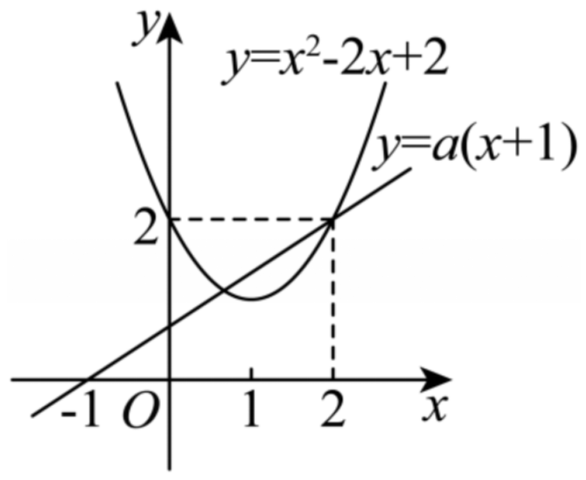
\includegraphics[width=0.30\textwidth]{figures/gao75_q12_graph.png}
\end{center}
% 原卷此处作“≥”，与题干严格不等号方向不一致，照录（见文件头“原卷笔误/存疑”①）
\step{由集合 $A$ 是“$2$ 集合”，故集合 $A$ 中只有一个元素，}
\step{得 $\begin{cases}2^2-2\times2+2\geqslant(2+1)a\\ 1^2-2\times1+2<(1+1)a\end{cases}$，解得 $\dfrac12<a\leqslant\dfrac23$，}
\step{故正实数 $a$ 的取值范围是 $\dfrac12<a\leqslant\dfrac23$.}
\solend
\fi

\end{enumerate}

\bigsec{二、选择题}

\begin{enumerate}
\setcounter{enumi}{12}

\item 已知全集 $U=\R$，集合 $A=\{x\mid x^2<4\}$，$B=\{y\mid y=x^2\}$，则图中阴影部分所表示的集合为\mbox{（\quad）}

\begin{center}
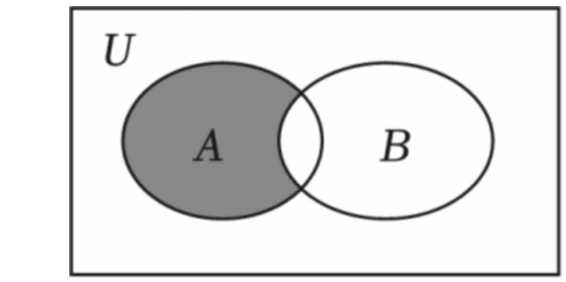
\includegraphics[width=0.26\textwidth]{figures/gao75_q13_venn.png}
\end{center}

\keepwithprev
A. $\{-2,-1,0\}$\qquad B. $(-\infty,4)$\qquad C. $(-2,0)$\qquad D. $(-2,0]$

\ifanswer
\solbegin
\step{集合 $A=\{x\mid x^2<4\}=(-2,2)$，$B=\{y\mid y=x^2\}=[0,+\infty)$，}
\step{图中阴影部分所表示的集合是 $A\cap\overline{B}=(-2,0)$. 故选 $C$.}
\solend
\fi

\item 已知 $x\in\R$，则“$\dfrac1x>1$”是“$x<1$”的\mbox{（\quad）}

\keepwithprev
A. 充分非必要条件\qquad B. 必要非充分条件\qquad C. 充要条件\qquad D. 既非充分又非必要条件

\ifanswer
\solbegin
\step{“$\dfrac1x>1$”$\Leftrightarrow0<x<1$，所以“$\dfrac1x>1$”是“$x<1$”的充分不必要条件. 故选 $A$.}
\solend
\fi

\item 已知集合 $M=\{x\mid x=m+\dfrac16,\,m\in\Z\}$，$N=\{x\mid x=\dfrac n2-\dfrac13,\,n\in\Z\}$，\\
$P=\{x\mid x=\dfrac p2+\dfrac16,\,p\in\Z\}$，则 $M$、$N$、$P$ 的关系为\mbox{（\quad）}

\keepwithprev
A. $M=N\subseteq P$\qquad B. $M\subseteq N=P$\qquad C. $M\subseteq N\subseteq P$\qquad D. $N\subseteq P\subseteq M$

\ifanswer
\solbegin
\step{集合 $N=\{x\mid x=\dfrac n2-\dfrac13,\,n\in\Z\}$，则 $x=\dfrac n2-\dfrac13=\dfrac{3n-2}6$，$n\in\Z$.}
\step{$P=\{x\mid x=\dfrac p2+\dfrac16,\,p\in\Z\}$，则 $x=\dfrac p2+\dfrac16=\dfrac{3p+1}6$，$p\in\Z$.}
\step{$M=\{x\mid x=m+\dfrac16,\,m\in\Z\}$，则 $x=m+\dfrac16=\dfrac{6m+1}6$，$m\in\Z$.}
\step{$M$、$N$、$P$ 三者分母相同，所以只需要比较他们的分子.}
\step{$M$：$6$ 的倍数$+1$，$N=P$：$3$ 的倍数$+1$，所以 $M\subseteq N=P$. 故选 $B$.}
\solend
\fi

\item 设集合 $P_1=\{x\mid x^2+ax+1>0\}$，$P_2=\{x\mid x^2+ax+2>0\}$，$Q_1=\{x\mid x^2+x+b>0\}$，$Q_2=\{x\mid x^2+2x+b>0\}$ 其中 $a,b\in\R$，给出下列两个命题：命题 $q_1$：对任意的 $a$，$P_1$ 是 $P_2$ 的子集；命题 $q_2$：对任意的 $b$，$Q_1$ 不是 $Q_2$ 的子集. 下列说法正确的是\mbox{（\quad）}

\keepwithprev
A. 命题 $q_1$ 是真命题，命题 $q_2$ 是假命题\qquad B. 命题 $q_1$ 是假命题，命题 $q_2$ 是真命题

C. 命题 $q_1$、$q_2$ 都是真命题\qquad D. 命题 $q_1$、$q_2$ 都是假命题

\ifanswer
\solbegin
\step{对于集合 $P_1=\{x\mid x^2+ax+1>0\}$，$P_2=\{x\mid x^2+ax+2>0\}$，}
\step{当 $m\in P_1$，即 $m^2+am+1>0$，得 $m^2+am+2>0$，}
\step{即有 $m\in P_2$，得对任意 $a$，$P_1$ 是 $P_2$ 的子集，命题 $q_1$ 为真命题；}
\step{当 $b=5$ 时，$Q_1=\{x\mid x^2+x+5>0\}=\R$，$Q_2=\{x\mid x^2+2x+5>0\}=\R$，}
\step{得 $Q_1$ 是 $Q_2$ 的子集；}
\step{存在 $b$，使得 $Q_1$ 是 $Q_2$ 的子集，故命题 $q_2$ 是假命题.}
\step{故选 $A$.}
\solend
\fi

\end{enumerate}

\bigsec{三、解答题}

\begin{enumerate}
\setcounter{enumi}{16}

\item 设集合 $A=\{x\mid x^2-2x=0\}$，$B=\{x\mid x^2+2(a+1)x+a^2-1=0\}$.

（1）写出集合 $A$ 的所有子集；

（2）若 $A\cap B=B$，求实数 $a$ 的取值范围.

\ifanswer
\solbegin
\stepm{(1)}{由 $x^2-2x=0$，得 $x=2$ 或 $x=0$，所以 $A=\{0,2\}$，}
\step{故集合 $A$ 的所有子集为 $\varnothing$、$\{0\}$、$\{2\}$、$\{0,2\}$.}
\stepm{(2)}{因为 $A\cap B=B$，所以 $B\subseteq A$，}
\step{方程 $x^2+2(a+1)x+a^2-1=0$，$\Delta=4(a+1)^2-4(a^2-1)=8a+8$，}
\step{若 $\Delta<0$，即 $a<-1$，方程 $x^2+2(a+1)x+a^2-1=0$ 无解，}
\step{此时 $B=\varnothing$，满足题意；}
\step{若 $\Delta=0$，即 $a=-1$，由 $x^2+2(a+1)x+a^2-1=0$，即 $x^2=0$，}
\step{解得 $x=0$，此时 $B=\{0\}$，满足题意；}
\step{若 $\Delta>0$，即 $a>-1$，要使 $B\subseteq A$，}
\step{则方程 $x^2+2(a+1)x+a^2-1=0$ 的解集为 $\{0,2\}$，}
\step{则 $\begin{cases}2+0=-2(a+1)\\ 2\times0=a^2-1\end{cases}$，$a$ 不存在.}
\step{综上所述，$a\leqslant-1$，即实数 $a$ 的取值范围为 $\{a\mid a\leqslant-1\}$.}
\solend
\fi

\ansspace

\item 已知全集 $U=\R$，集合 $A=\left\{x\,\middle|\,\dfrac{x-1}{x-3}<0\right\}$，$B=\{x\mid|x-a|<2\}$.

（1）当 $a=1$ 时，试用区间表示集合 $A$、$B$；

（2）若 $A\cup B=B$，求实数 $a$ 的取值范围.

\ifanswer
\solbegin
\stepm{(1)}{不等式 $\dfrac{x-1}{x-3}<0$ 可化为 $(x-1)(x-3)<0$，解得 $1<x<3$，即 $A=(1,3)$，}
\step{当 $a=1$ 时，$|x-1|<2$，则 $-2<x-1<2$，解得 $-1<x<3$，}
\step{即 $B=(-1,3)$；}
\stepm{(2)}{由不等式 $|x-a|<2$ 得 $-2<x-a<2$，解得 $-2+a<x<2+a$，}
\step{即 $B=\{x\mid-2+a<x<2+a\}$，}
\step{因为 $A\cup B=B$，所以 $A\subseteq B$，则 $\begin{cases}-2+a\leqslant1\\ 2+a\geqslant3\end{cases}$，解得 $1\leqslant a\leqslant3$，}
\step{即实数 $a$ 的取值范围为 $[1,3]$.}
\solend
\fi

\ansspace

\item 法国数学家弗朗索瓦·韦达 1615 年在著作《论方程的识别与订正》中建立了方程根与系数的关系. 发现一元二次方程 $ax^2+bx+c=0$，$a\neq0$ 的根与系数有如下的关系：

$x_1+x_2=-\dfrac ba$，$x_1x_2=\dfrac ca$，此即为韦达定理. 韦达定理的逆定理仍成立：如果两个数 $x_1$，$x_2$ 满足 $x_1+x_2=-\dfrac ba$，$x_1x_2=\dfrac ca$，则这两个数 $x_1$、$x_2$ 是方程 $ax^2+bx+c=0$，$a\neq0$ 的两个根. 例如：$m+n=-3$，$mn=2$，则 $m$、$n$ 是方程 $x^2+3x+2=0$ 的两个根. 请根据上述材料解决以下问题.

（1）已知 $m$、$n$ 是两个不相等的实数，满足 $m^2-6m-5=0$，$n^2-6n-5=0$，求 $\dfrac1m+\dfrac1n$ 的值；

（2）已知实数 $x$、$y$ 满足 $x+y+xy=17$，$x^2y+xy^2=72$，求 $x^2+y^2$ 的值.

\ifanswer
\solbegin
\stepm{(1)}{由题意，不相等的实数 $m$、$n$ 满足 $m^2-6m-5=0$、$n^2-6n-5=0$，}
\step{因此 $m$、$n$ 是一元二次方程 $x^2-6x-5=0$ 的两个不等实根.}
\step{由韦达定理得 $m+n=6$，$mn=-5$，因此 $\dfrac1m+\dfrac1n=\dfrac{m+n}{mn}=\dfrac6{-5}=-\dfrac65$.}
\stepm{(2)}{令 $s=x+y$，$t=xy$，}
\step{因为 $x+y+xy=17$，$x^2y+xy^2=72$，}
\step{即 $x+y+xy=17$，$xy(x+y)=72$，将已知条件变形得 $\begin{cases}s+t=17\\ st=72\end{cases}$.}
\step{由韦达定理逆定理，$s$、$t$ 是一元二次方程 $z^2-17z+72=0$ 的两个实根，}
\step{解方程得 $z_1=8$，$z_2=9$，即有两组解 $\begin{cases}s=8\\ t=9\end{cases}$ 和 $\begin{cases}s=9\\ t=8\end{cases}$.}
\step{当 $\begin{cases}s=8\\ t=9\end{cases}$ 时，$x$、$y$ 是方程 $w^2-8w+9=0$ 的根，}
\step{判别式 $\Delta=8^2-4\times1\times9=64-36=28>0$，符合题意，}
\step{此时 $x^2+y^2=(x+y)^2-2xy=s^2-2t=8^2-2\times9=64-18=46$；}
\step{当 $\begin{cases}s=9\\ t=8\end{cases}$ 时，$x$、$y$ 是方程 $w^2-9w+8=0$ 的根，}
\step{判别式 $\Delta=9^2-4\times1\times8=81-32=49>0$，符合题意，}
\step{此时 $x^2+y^2=(x+y)^2-2xy=s^2-2t=9^2-2\times8=81-16=65$.}
\step{综上，$x^2+y^2$ 的值为 $46$ 或 $65$.}
\solend
\fi

\ansspace

\item 已知关于 $x$ 的不等式 $ax^2-(a+1)x+b<0$.

（1）若不等式的解集是 $\{x\mid1<x<5\}$，求 $a+b$ 的值；

（2）若 $b=-\dfrac12$ 且不等式的解集为 $\R$，求 $a$ 取值范围；

（3）若 $b=1$，讨论此不等式的解集.

\ifanswer
\solbegin
\stepm{(1)}{由题意得 $1$ 和 $5$ 是方程 $ax^2-(a+1)x+b=0$ 的两个根且 $a>0$，}
\step{所以 $1+5=\dfrac{a+1}a$，$1\times5=\dfrac ba$，解得 $a=\dfrac15$，$b=1$，所以 $a+b=\dfrac65$.}
\stepm{(2)}{若 $b=-\dfrac12$，则不等式为 $ax^2-(a+1)x-\dfrac12<0$，}
\step{当 $a\neq0$，则有 $\begin{cases}a<0\\ \Delta=(a+1)^2+2a<0\end{cases}$，解得 $-2-\sqrt3<a<-2+\sqrt3$；}
\step{当 $a=0$，不等式即为 $-x-\dfrac12<0$，则 $x>-\dfrac12$，不合题意；}
\step{所以 $a$ 的取值范围是 $(-2-\sqrt3,-2+\sqrt3)$.}
\stepm{(3)}{若 $b=1$，则不等式为 $ax^2-(a+1)x+1<0$，即 $(ax-1)(x-1)<0$.}
\step{当 $a\neq0$ 时，由 $ax^2-(a+1)x+1<0$ 得 $(ax-1)(x-1)<0$.}
\step{方程 $(ax-1)(x-1)=0$ 的根为 $x=\dfrac1a$ 或 $x=1$，}
\step{当 $0<a<1$ 时，$\dfrac1a>1$，则不等式的解集为 $\left(1,\dfrac1a\right)$；}
\step{当 $a<0$ 时，$\dfrac1a<1$，则不等式的解集为 $\left(-\infty,\dfrac1a\right)\cup(1,+\infty)$；}
\step{当 $a=1$ 时，不等式即为 $(x-1)^2<0$，则不等式的解集为 $\varnothing$；}
\step{当 $a>1$ 时，$\dfrac1a<1$，则不等式的解集为 $\left(\dfrac1a,1\right)$；}
\step{当 $a=0$ 时，不等式为 $-x+1<0$，则不等式的解集为 $(1,+\infty)$；}
\step{综上所述，当 $a<0$ 时，不等式的解集为 $\left(-\infty,\dfrac1a\right)\cup(1,+\infty)$；}
\step{当 $a=0$ 时，不等式的解集为 $(1,+\infty)$；}
\step{当 $0<a<1$ 时，不等式的解集为 $\left(1,\dfrac1a\right)$；}
\step{当 $a=1$ 时，不等式的解集为 $\varnothing$；}
\step{当 $a>1$ 时，不等式的解集为 $\left(\dfrac1a,1\right)$.}
\solend
\fi

\ansspace

\item 已知关于 $x$ 的不等式① $x^2+2cx+c>0$，② $x^2+cx+c^2-1>0$，其中 $c$ 是实数.

（1）若 $1$ 是不等式②的一个解，求实数 $c$ 的取值范围；

（2）证明：不等式①、②中至多有一个恒成立；

（3）当 $c=0$ 时，“$x$ 满足 $|mx^2-4x+3|>5$”的一个必要非充分条件是“$x$ 满足 $x^2+cx+c^2-1>0$，求实数 $m$ 的取值范围.

\ifanswer
\solbegin
\stepm{(1)}{因为 $1$ 是不等式②的一个解，所以 $1+c+c^2-1>0$，}
\step{即 $c(c+1)>0$，解得 $c>0$ 或 $c<-1$，}
\step{所以实数 $c$ 的取值范围为 $(-\infty,-1)\cup(0,+\infty)$.}
\stepm{(2)}{假设不等式①、②都恒成立，}
\step{不等式① $x^2+2cx+c>0$ 恒成立，所以 $4c^2-4c<0$，所以 $0<c<1$；}
\step{② $x^2+cx+c^2-1>0$ 恒成立，所以 $c^2-4(c^2-1)<0$，$c^2>\dfrac43$，}
\step{解得 $c>\dfrac{2\sqrt3}3$ 或 $c<-\dfrac{2\sqrt3}3$；}
\step{所以当不等式①、②都恒成立时，}
\step{不等式组 $\begin{cases}0<c<1\\ c\in\left(-\infty,-\dfrac{2\sqrt3}3\right)\cup\left(\dfrac{2\sqrt3}3,+\infty\right)\end{cases}$ 无解，}
\step{所以假设不成立，}
\step{所以不等式①、②中至多有一个恒成立.}
\stepm{(3)}{当 $c=0$ 时，由 $x^2+cx+c^2-1>0$ 得 $x^2-1>0$，}
\step{解集为 $(-\infty,-1)\cup(1,+\infty)$.}
\step{记集合 $A=\{x\mid|mx^2-4x+3|>5\}$，集合 $B=\{x\mid x<-1\text{ 或 }x>1\}$.}
\step{由“$x$ 满足 $|mx^2-4x+3|>5$”的一个必要非充分条件是}
\step{“$x$ 满足 $x^2+cx+c^2-1>0$”得 $A$ 是 $B$ 的真子集.}
\step{所以 $\overline{B}$ 是 $A$ 的真子集，即对任意 $x\in[-1,1]$，$|mx^2-4x+3|\leqslant5$ 恒成立.}
\step{当 $x=0$ 时，不等式 $-5\leqslant mx^2-4x+3\leqslant5$ 恒成立；}
\step{当 $x\in[-1,0)\cup(0,1]$ 时，}
\step{则 $mx^2-4x+3\geqslant-5$ 与 $mx^2-4x+3\leqslant5$ 同时成立.}
\step{①由 $mx^2-4x+3\geqslant-5$，得 $m\geqslant\dfrac{4x-8}{x^2}$，求值域得 $\dfrac{4x-8}{x^2}$ 的最大值 $=-4$，}
\step{所以 $m\geqslant-4$.}
\step{②由 $mx^2-4x+3\leqslant5$，得 $m\leqslant\dfrac{4x+2}{x^2}$，求值域得 $\dfrac{4x+2}{x^2}$ 的最小值 $=-2$，}
\step{所以 $m\leqslant-2$.}
\step{综上所述，实数 $m$ 的取值范围为 $[-4,-2]$.}
\solend
\fi

\ansspace*[7]

\end{enumerate}

\end{document}
"
% 紧凑版：xelatex "\def\iscompact{1}% 高一75_市二中学_10月月考.tex
%   —— 高一上数学“2026-2027 年市二中学高一上 10 月月考”（讲评版）
% 试卷版：xelatex 高一75_市二中学_10月月考.tex
% 答案版：xelatex "\def\isanswer{1}\input{高一75_市二中学_10月月考.tex}"
% 紧凑版：xelatex "\def\iscompact{1}\input{高一75_市二中学_10月月考.tex}"
%
% 原始材料：微信公众号“魔都数学加油站”文章，连载“27学年高一75”；
% 原文标题“27学年高一75——2026-2027年上海市市二中学高一上10月月考”；
% 原文链接：https://mp.weixin.qq.com/s/dhxtwWEZgKLxeKdkbWqOhw。
% 页面标注发布时间 2026-10-22 21:45（上海）。
% 正文为 11 张 PNG 页（`原图/高一75_市二中学_10月月考/01..11.png`）：
% 第 2、4、5、6、9 页为 4762×6735，其余 6 页为 2560×3620，均按页序读取。
% 11 页全为试卷正文页（卷首标题在第 1 页页顶，卷末第 21 题 (3) 解析止于第 11 页），
% 无封面页、目录页、二维码或宣传页。粉色斜排“魔都数学加油站”为卷面水印，未录入。
%
% 卷首标题：照卷面印作“2026-2027 年市二中学高一上 10 月月考”（黑体加粗一行）。
% 原卷年份区间用半角连字符，本稿按全稿惯例排 en dash；原卷无副标题。
%
% 篇幅与题号：原卷自第 3 题起编号（第 1、2 题不在本卷内）。填空题 3—12（10 题）、
% 选择题 13—16（4 题）、解答题 17—21（5 题），共 19 题。本稿沿用原节与原题号，
% 只改排为全稿统一的大节样式。
%
% 讲评版：原卷第 4 题只印【答案】（“$[-1,2]$”），本稿只给 \ans{}；其余 18 题均印
% 【解析】，用 \solbegin…\solend。四道选择题的作答括号原卷即留空，答案写在解析末句
% “故选 C／A／B／A”，照录在解析内，不另提 \ans{}。
%
% 副标题：原卷未印副标题。本稿按“知识模块”口径标作“集合与常用逻辑用语、不等式”：
% 19 题中集合与常用逻辑用语 9 题（第 3、4、5、8、10、12、13、15、17、18 题中的集合题），
% 不等式 10 题（第 6、7、9、11、19、20、21 题及第 12、20 题的不等式部分），两类均确有
% 分量，故并标。口径同 高一63、高一68—74。
%
% 与原卷的排版差异：
%   ① 原卷每题下直接印【答案】/【解析】，本稿按全稿惯例将答案与解析置于答案版；
%   ② 原卷未印副标题，本稿按“知识模块”口径补出；
%   ③ 原卷填空横线约四个字宽，本稿按全稿惯例统一排 \blankline[4.4em]；
%   ④ 原卷数集记号排粗体 $\mathbf{R}$（第 5、6、7、9、10、14、18、20、21 题），本稿
%      按全稿惯例改用 $\R$（同 高一68—74）；第 11 题的“解集为 $\R$”同此；
%   ⑤ 原卷句末标点多为西文句点，均逐处照录；
%   ⑥ 第 17—21 题的子问原卷印作“（1）…（2）…”，本稿按 高一69—74 成例用行内
%      “（1）（2）（3）”段，解析中的子问标号用 \stepm{(1)}{…}；
%   ⑦ 每道解答题原卷未留作答空白，本稿按全稿惯例加 \ansspace（末题用 \ansspace*）；
%   ⑧ 选择题的作答括号原卷排半角“(    )”，本稿按全稿惯例排 \mbox{（\quad）}；
%      选项行排照原卷——第 13、14 题一行四条，第 15、16 题一行四条；
%   ⑨ 第 9、12、15、17—21 题解析中的不等式组／方程组，原卷均排作“{”连接的多行式，
%      本稿按全稿惯例排 cases；
%   ⑩ 第 12 题解析有一幅“抛物线 + 直线”图：原卷印在解析第 3 行右侧、题干无“如图”二字
%      （解析里写“两函数图象如图：”）。本稿按原卷截图裁取（`figures/gao75_q12_graph.png`，
%      由第 3 页原图裁出、去除粉色水印后转灰度，未放大），放在答案版解析第 3 条之后；
%   ⑪ 第 13 题题干中间有一幅韦恩图（全集矩形内含 A、B 两圆，A 涂灰）：原卷印在题干
%      右侧、题干句子被图隔开。本稿按原卷截图裁取（`figures/gao75_q13_venn.png`，由第 3
%      页原图裁出、去除粉色水印后转灰度，并抹去左侧侵入的“分”字），放在题干之后、
%      选项之前，仅答案版出。
%
% 原卷笔误/存疑（均照录未改，正文对应处另有 % 注）：
%   ① 第 12 题解析列不等式组时写 $2^2-2\times2+2\geqslant(2+1)a$，与
%      $x^2-2x+2<a(x+1)$ 的严格不等号方向不一致；原卷如此，照录未改。
%   ② 第 14 题选项 A—D 的“充分非必要”“必要非充分”“既非充分又非必要”与原卷
%      其它题的“充分不必要”写法不同，照录未统一。
%   ④ 第 21 题 (3) 题干的“$x$ 满足 $|mx^2-4x+3|>5$”的一个必要非充分条件是
%      “$x$ 满足 $x^2+cx+c^2-1>0$，原卷只有左引号、无右引号（且逗号在引号内），
%      本稿照录未补。
%   ③ 第 20 题 (2) 的解集写成 $(-2-\sqrt3,-2+\sqrt3)$，其中 $a<0$ 与 $\Delta<0$ 联立后
%      左端点应为 $-2-\sqrt3$、右端点为 $-2+\sqrt3$；原卷如此，照录未改。
%
% 行数核对：逐题数 \step/\stepm 条数与原卷【解析】印刷行数，18 题逐一相符，
% 合计 132 条 / 132 行（Q3：6；Q5：1；Q6：2；Q7：1；Q8：2；Q9：3；Q10：10；
% Q11：8；Q12：6；Q13：2；Q14：1；Q15：5；Q16：7；Q17：12；Q18：7；Q19：15；
% Q20：19；Q21：25）。另第 4 题只印【答案】，提 \ans{}，不计入 \step 账。
%
% 插图：第 12 题解析的抛物线图、第 13 题题干的韦恩图，见上⑩⑪；其余题干无配图。
%
\documentclass[a4paper,11pt]{article}
\usepackage{common}

\begin{document}

\examtitlest[3]{2026--2027 年市二中学高一上 10 月月考}{集合与常用逻辑用语、不等式}

\bigsec{一、填空题}

\begin{enumerate}
\setcounter{enumi}{2}

\item 已知集合 $A=\{a,a^2\}$，且 $1\in A$，则 $a=$\blankline[4.4em].

\ifanswer
\solbegin
\step{因为 $1\in A=\{a,a^2\}$，所以 $a=1$ 或 $a^2=1$.}
\step{又集合 $A=\{a,a^2\}$ 是用列举法写出两个元素的，其元素必须互异，故 $a\neq a^2$，}
\step{即 $a\neq0$ 且 $a\neq1$，所以 $a=1$ 应舍去；}
\step{由 $a^2=1$ 得 $a=1$（舍去）或 $a=-1$.}
\step{当 $a=-1$ 时，$A=\{-1,1\}$，满足 $1\in A$ 且两个元素互异.}
\step{故 $a=-1$.}
\solend
\fi

\item 已知集合 $A=[-1,1]$，$B=[0,2]$，则 $A\cup B=$\blankline[4.4em].

\ifanswer
\ans{$[-1,2]$}
\fi

\item 已知全集 $U=\R$，集合 $A=\{x\mid x\neq1\}$，则 $\overline{A}=$\blankline[4.4em].

\ifanswer
\solbegin
\step{因为全集 $U=\R$，集合 $A=\{x\mid x\neq1\}$，所以 $\overline{A}=\{x\mid x=1\}$.}
\solend
\fi

\item 设 $x\in\R$，不等式 $x^2-4x<0$ 的解集用区间表示是\blankline[4.4em].

\ifanswer
\solbegin
\step{因为 $x^2-4x<0$，即 $x(x-4)<0$，所以 $0<x<4$，}
\step{所以 $x(x-4)<0$ 的解集为 $(0,4)$.}
\solend
\fi

\item 已知 $m\in\R$，若关于 $x$ 的方程 $2mx^2+3x+m-1=m^2\cdot x^2+(m+1)x+1$ 解集为 $\R$，则 $m$ 的值为\blankline[4.4em].

\ifanswer
\solbegin
\step{由题意得 $2m=m^2$，$3=m+1$，$m-1=1$，所以 $m=2$.}
\solend
\fi

\item 设 $\alpha:x\leqslant m$，$\beta:|x-2|\leqslant1$，若 $\alpha$ 是 $\beta$ 的必要条件，则实数 $m$ 的取值范围是\blankline[4.4em].

\ifanswer
\solbegin
\step{由 $|x-2|\leqslant1$，得 $-1\leqslant x-2\leqslant1$，解得 $1\leqslant x\leqslant3$，}
\step{因为 $\alpha$ 是 $\beta$ 的必要条件，所以 $\{x\mid1\leqslant x\leqslant3\}\subseteq\{x\mid x\leqslant m\}$，得 $m\geqslant3$.}
\solend
\fi

\item 设 $a\in\R$，若关于 $x$ 的不等式 $\dfrac{a}{x-1}\leqslant1$ 的解集是 $(-\infty,1)\cup[2,+\infty)$，则 $a$ 的值为\blankline[4.4em].

\ifanswer
\solbegin
\step{不等式可变形为 $\dfrac{a+1-x}{x-1}\leqslant0$，等价于 $\begin{cases}(a+1-x)(x-1)\leqslant0\\ x-1\neq0\end{cases}$，}
\step{因为原不等式的解集是 $(-\infty,1)\cup[2,+\infty)$，}
\step{所以 $1$，$2$ 是方程 $(a+1-x)(x-1)=0$ 的两根，所以 $a+1=2$，解得 $a=1$.}
\solend
\fi

\item 下列命题：① “$x>1$ 或 $y>1$”的否定形式是“$x\leqslant1$ 或 $y\leqslant1$”，② 若 $A\cup B=B$，则 $A\subseteq B$，③ 方程 $ax+1=0$ 的解是 $x=-\frac1a$，④ “$ac=bc$”是“$a=b$”的必要非充分条件，⑤ “任意 $x\in\R$，$f(x)=f(-x)$”的否定形式是“存在 $x_0\in\R$，使得 $f(x_0)\neq f(-x_0)$”其中真命题的序号是\blankline[4.4em]（填写序号）.

\ifanswer
\solbegin
\step{①假命题：“$x>1$ 或 $y>1$”的否定形式是“$x\leqslant1$ 且 $y\leqslant1$”；}
\step{②真命题：$A\cup B=B\Leftrightarrow A\subseteq B$；}
\step{③假命题：当 $a=0$ 时，方程无解，因此该命题忽略了 $a=0$ 的情况；}
\step{④真命题：先判断必要性：若 $a=b$，则有 $ac=bc$，所以必要性成立；}
\step{再判断充分性：若 $ac=bc$，即 $(a-b)c=0$，当 $c=0$ 时，$a$ 和 $b$ 可以不相等，}
\step{因此充分性不成立.}
\step{⑤真命题：全称命题的否定是存在量词命题，}
\step{“任意 $x\in\R$，$f(x)=f(-x)$”的否定形式是}
\step{“存在 $x_0\in\R$，使得 $f(x_0)\neq f(-x_0)$”，表述正确.}
\step{故正确的是②④⑤.}
\solend
\fi

\item 为了加强家校联系，蔡老师组建了一个由学生、家长和教师组成的微信群. 已知该群中男学生人数多于女学生人数，女学生人数多于家长人数，家长人数多于教师人数，教师人数的两倍多于男学生人数. 则该微信群人数的最小值为\blankline[4.4em].

\ifanswer
\solbegin
\step{设男学生、女学生、家长、教师的人数分别为 $M$、$F$、$P$、$T$，}
\step{它们都是正整数.}
\step{由题意得 $M>F>P>T$，且教师人数的两倍多于男学生人数，即 $2T>M$.}
\step{由 $M>F>P>T$ 得 $M\geqslant T+3$；}
\step{又 $2T>M\geqslant T+3$，所以 $2T>T+3$，解得 $T>3$，故教师人数最少为 $T=4$.}
\step{当 $T=4$ 时，为使总人数最少，取 $P=5$、$F=6$、$M=7$，}
\step{此时 $7>6>5>4$ 且 $2\times4=8>7$，满足题意.}
\step{于是微信群人数为 $4+5+6+7=22$，所以该微信群人数的最小值为 $22$.}
\solend
\fi

\item 若集合 $M$ 有 $k$ 个子集，则称集合 $M$ 为“$k$ 集合”，\\
已知集合 $A=\{x\mid x^2-(a+2)x+2-a<0,\,x\in\Z\}$ 是“$2$ 集合”，则正实数 $a$ 的取值范围是\blankline[4.4em].

\ifanswer
\solbegin
\step{由 $x^2-(a+2)x+2-a<0$，得 $x^2-2x+2<a(x+1)$，}
\step{设二次函数 $y=x^2-2x+2$ 与一次函数 $y=a(x+1)$，}
\needvspace{13\baselineskip}
\step{由 $a>0$，$y=a(x+1)$ 过定点 $(-1,0)$，两函数图象如图：}
\begin{center}
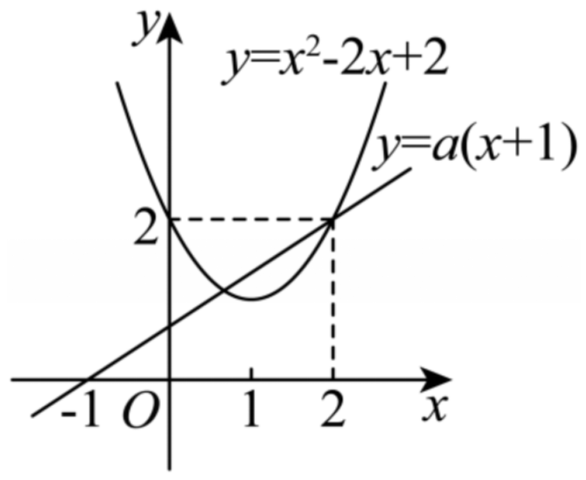
\includegraphics[width=0.30\textwidth]{figures/gao75_q12_graph.png}
\end{center}
% 原卷此处作“≥”，与题干严格不等号方向不一致，照录（见文件头“原卷笔误/存疑”①）
\step{由集合 $A$ 是“$2$ 集合”，故集合 $A$ 中只有一个元素，}
\step{得 $\begin{cases}2^2-2\times2+2\geqslant(2+1)a\\ 1^2-2\times1+2<(1+1)a\end{cases}$，解得 $\dfrac12<a\leqslant\dfrac23$，}
\step{故正实数 $a$ 的取值范围是 $\dfrac12<a\leqslant\dfrac23$.}
\solend
\fi

\end{enumerate}

\bigsec{二、选择题}

\begin{enumerate}
\setcounter{enumi}{12}

\item 已知全集 $U=\R$，集合 $A=\{x\mid x^2<4\}$，$B=\{y\mid y=x^2\}$，则图中阴影部分所表示的集合为\mbox{（\quad）}

\begin{center}
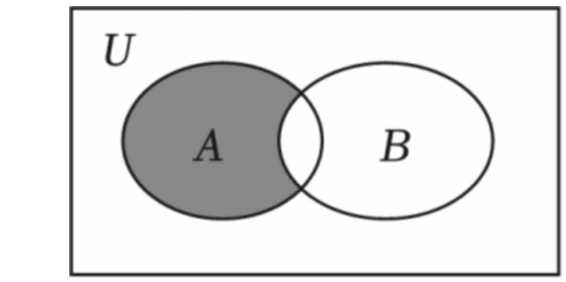
\includegraphics[width=0.26\textwidth]{figures/gao75_q13_venn.png}
\end{center}

\keepwithprev
A. $\{-2,-1,0\}$\qquad B. $(-\infty,4)$\qquad C. $(-2,0)$\qquad D. $(-2,0]$

\ifanswer
\solbegin
\step{集合 $A=\{x\mid x^2<4\}=(-2,2)$，$B=\{y\mid y=x^2\}=[0,+\infty)$，}
\step{图中阴影部分所表示的集合是 $A\cap\overline{B}=(-2,0)$. 故选 $C$.}
\solend
\fi

\item 已知 $x\in\R$，则“$\dfrac1x>1$”是“$x<1$”的\mbox{（\quad）}

\keepwithprev
A. 充分非必要条件\qquad B. 必要非充分条件\qquad C. 充要条件\qquad D. 既非充分又非必要条件

\ifanswer
\solbegin
\step{“$\dfrac1x>1$”$\Leftrightarrow0<x<1$，所以“$\dfrac1x>1$”是“$x<1$”的充分不必要条件. 故选 $A$.}
\solend
\fi

\item 已知集合 $M=\{x\mid x=m+\dfrac16,\,m\in\Z\}$，$N=\{x\mid x=\dfrac n2-\dfrac13,\,n\in\Z\}$，\\
$P=\{x\mid x=\dfrac p2+\dfrac16,\,p\in\Z\}$，则 $M$、$N$、$P$ 的关系为\mbox{（\quad）}

\keepwithprev
A. $M=N\subseteq P$\qquad B. $M\subseteq N=P$\qquad C. $M\subseteq N\subseteq P$\qquad D. $N\subseteq P\subseteq M$

\ifanswer
\solbegin
\step{集合 $N=\{x\mid x=\dfrac n2-\dfrac13,\,n\in\Z\}$，则 $x=\dfrac n2-\dfrac13=\dfrac{3n-2}6$，$n\in\Z$.}
\step{$P=\{x\mid x=\dfrac p2+\dfrac16,\,p\in\Z\}$，则 $x=\dfrac p2+\dfrac16=\dfrac{3p+1}6$，$p\in\Z$.}
\step{$M=\{x\mid x=m+\dfrac16,\,m\in\Z\}$，则 $x=m+\dfrac16=\dfrac{6m+1}6$，$m\in\Z$.}
\step{$M$、$N$、$P$ 三者分母相同，所以只需要比较他们的分子.}
\step{$M$：$6$ 的倍数$+1$，$N=P$：$3$ 的倍数$+1$，所以 $M\subseteq N=P$. 故选 $B$.}
\solend
\fi

\item 设集合 $P_1=\{x\mid x^2+ax+1>0\}$，$P_2=\{x\mid x^2+ax+2>0\}$，$Q_1=\{x\mid x^2+x+b>0\}$，$Q_2=\{x\mid x^2+2x+b>0\}$ 其中 $a,b\in\R$，给出下列两个命题：命题 $q_1$：对任意的 $a$，$P_1$ 是 $P_2$ 的子集；命题 $q_2$：对任意的 $b$，$Q_1$ 不是 $Q_2$ 的子集. 下列说法正确的是\mbox{（\quad）}

\keepwithprev
A. 命题 $q_1$ 是真命题，命题 $q_2$ 是假命题\qquad B. 命题 $q_1$ 是假命题，命题 $q_2$ 是真命题

C. 命题 $q_1$、$q_2$ 都是真命题\qquad D. 命题 $q_1$、$q_2$ 都是假命题

\ifanswer
\solbegin
\step{对于集合 $P_1=\{x\mid x^2+ax+1>0\}$，$P_2=\{x\mid x^2+ax+2>0\}$，}
\step{当 $m\in P_1$，即 $m^2+am+1>0$，得 $m^2+am+2>0$，}
\step{即有 $m\in P_2$，得对任意 $a$，$P_1$ 是 $P_2$ 的子集，命题 $q_1$ 为真命题；}
\step{当 $b=5$ 时，$Q_1=\{x\mid x^2+x+5>0\}=\R$，$Q_2=\{x\mid x^2+2x+5>0\}=\R$，}
\step{得 $Q_1$ 是 $Q_2$ 的子集；}
\step{存在 $b$，使得 $Q_1$ 是 $Q_2$ 的子集，故命题 $q_2$ 是假命题.}
\step{故选 $A$.}
\solend
\fi

\end{enumerate}

\bigsec{三、解答题}

\begin{enumerate}
\setcounter{enumi}{16}

\item 设集合 $A=\{x\mid x^2-2x=0\}$，$B=\{x\mid x^2+2(a+1)x+a^2-1=0\}$.

（1）写出集合 $A$ 的所有子集；

（2）若 $A\cap B=B$，求实数 $a$ 的取值范围.

\ifanswer
\solbegin
\stepm{(1)}{由 $x^2-2x=0$，得 $x=2$ 或 $x=0$，所以 $A=\{0,2\}$，}
\step{故集合 $A$ 的所有子集为 $\varnothing$、$\{0\}$、$\{2\}$、$\{0,2\}$.}
\stepm{(2)}{因为 $A\cap B=B$，所以 $B\subseteq A$，}
\step{方程 $x^2+2(a+1)x+a^2-1=0$，$\Delta=4(a+1)^2-4(a^2-1)=8a+8$，}
\step{若 $\Delta<0$，即 $a<-1$，方程 $x^2+2(a+1)x+a^2-1=0$ 无解，}
\step{此时 $B=\varnothing$，满足题意；}
\step{若 $\Delta=0$，即 $a=-1$，由 $x^2+2(a+1)x+a^2-1=0$，即 $x^2=0$，}
\step{解得 $x=0$，此时 $B=\{0\}$，满足题意；}
\step{若 $\Delta>0$，即 $a>-1$，要使 $B\subseteq A$，}
\step{则方程 $x^2+2(a+1)x+a^2-1=0$ 的解集为 $\{0,2\}$，}
\step{则 $\begin{cases}2+0=-2(a+1)\\ 2\times0=a^2-1\end{cases}$，$a$ 不存在.}
\step{综上所述，$a\leqslant-1$，即实数 $a$ 的取值范围为 $\{a\mid a\leqslant-1\}$.}
\solend
\fi

\ansspace

\item 已知全集 $U=\R$，集合 $A=\left\{x\,\middle|\,\dfrac{x-1}{x-3}<0\right\}$，$B=\{x\mid|x-a|<2\}$.

（1）当 $a=1$ 时，试用区间表示集合 $A$、$B$；

（2）若 $A\cup B=B$，求实数 $a$ 的取值范围.

\ifanswer
\solbegin
\stepm{(1)}{不等式 $\dfrac{x-1}{x-3}<0$ 可化为 $(x-1)(x-3)<0$，解得 $1<x<3$，即 $A=(1,3)$，}
\step{当 $a=1$ 时，$|x-1|<2$，则 $-2<x-1<2$，解得 $-1<x<3$，}
\step{即 $B=(-1,3)$；}
\stepm{(2)}{由不等式 $|x-a|<2$ 得 $-2<x-a<2$，解得 $-2+a<x<2+a$，}
\step{即 $B=\{x\mid-2+a<x<2+a\}$，}
\step{因为 $A\cup B=B$，所以 $A\subseteq B$，则 $\begin{cases}-2+a\leqslant1\\ 2+a\geqslant3\end{cases}$，解得 $1\leqslant a\leqslant3$，}
\step{即实数 $a$ 的取值范围为 $[1,3]$.}
\solend
\fi

\ansspace

\item 法国数学家弗朗索瓦·韦达 1615 年在著作《论方程的识别与订正》中建立了方程根与系数的关系. 发现一元二次方程 $ax^2+bx+c=0$，$a\neq0$ 的根与系数有如下的关系：

$x_1+x_2=-\dfrac ba$，$x_1x_2=\dfrac ca$，此即为韦达定理. 韦达定理的逆定理仍成立：如果两个数 $x_1$，$x_2$ 满足 $x_1+x_2=-\dfrac ba$，$x_1x_2=\dfrac ca$，则这两个数 $x_1$、$x_2$ 是方程 $ax^2+bx+c=0$，$a\neq0$ 的两个根. 例如：$m+n=-3$，$mn=2$，则 $m$、$n$ 是方程 $x^2+3x+2=0$ 的两个根. 请根据上述材料解决以下问题.

（1）已知 $m$、$n$ 是两个不相等的实数，满足 $m^2-6m-5=0$，$n^2-6n-5=0$，求 $\dfrac1m+\dfrac1n$ 的值；

（2）已知实数 $x$、$y$ 满足 $x+y+xy=17$，$x^2y+xy^2=72$，求 $x^2+y^2$ 的值.

\ifanswer
\solbegin
\stepm{(1)}{由题意，不相等的实数 $m$、$n$ 满足 $m^2-6m-5=0$、$n^2-6n-5=0$，}
\step{因此 $m$、$n$ 是一元二次方程 $x^2-6x-5=0$ 的两个不等实根.}
\step{由韦达定理得 $m+n=6$，$mn=-5$，因此 $\dfrac1m+\dfrac1n=\dfrac{m+n}{mn}=\dfrac6{-5}=-\dfrac65$.}
\stepm{(2)}{令 $s=x+y$，$t=xy$，}
\step{因为 $x+y+xy=17$，$x^2y+xy^2=72$，}
\step{即 $x+y+xy=17$，$xy(x+y)=72$，将已知条件变形得 $\begin{cases}s+t=17\\ st=72\end{cases}$.}
\step{由韦达定理逆定理，$s$、$t$ 是一元二次方程 $z^2-17z+72=0$ 的两个实根，}
\step{解方程得 $z_1=8$，$z_2=9$，即有两组解 $\begin{cases}s=8\\ t=9\end{cases}$ 和 $\begin{cases}s=9\\ t=8\end{cases}$.}
\step{当 $\begin{cases}s=8\\ t=9\end{cases}$ 时，$x$、$y$ 是方程 $w^2-8w+9=0$ 的根，}
\step{判别式 $\Delta=8^2-4\times1\times9=64-36=28>0$，符合题意，}
\step{此时 $x^2+y^2=(x+y)^2-2xy=s^2-2t=8^2-2\times9=64-18=46$；}
\step{当 $\begin{cases}s=9\\ t=8\end{cases}$ 时，$x$、$y$ 是方程 $w^2-9w+8=0$ 的根，}
\step{判别式 $\Delta=9^2-4\times1\times8=81-32=49>0$，符合题意，}
\step{此时 $x^2+y^2=(x+y)^2-2xy=s^2-2t=9^2-2\times8=81-16=65$.}
\step{综上，$x^2+y^2$ 的值为 $46$ 或 $65$.}
\solend
\fi

\ansspace

\item 已知关于 $x$ 的不等式 $ax^2-(a+1)x+b<0$.

（1）若不等式的解集是 $\{x\mid1<x<5\}$，求 $a+b$ 的值；

（2）若 $b=-\dfrac12$ 且不等式的解集为 $\R$，求 $a$ 取值范围；

（3）若 $b=1$，讨论此不等式的解集.

\ifanswer
\solbegin
\stepm{(1)}{由题意得 $1$ 和 $5$ 是方程 $ax^2-(a+1)x+b=0$ 的两个根且 $a>0$，}
\step{所以 $1+5=\dfrac{a+1}a$，$1\times5=\dfrac ba$，解得 $a=\dfrac15$，$b=1$，所以 $a+b=\dfrac65$.}
\stepm{(2)}{若 $b=-\dfrac12$，则不等式为 $ax^2-(a+1)x-\dfrac12<0$，}
\step{当 $a\neq0$，则有 $\begin{cases}a<0\\ \Delta=(a+1)^2+2a<0\end{cases}$，解得 $-2-\sqrt3<a<-2+\sqrt3$；}
\step{当 $a=0$，不等式即为 $-x-\dfrac12<0$，则 $x>-\dfrac12$，不合题意；}
\step{所以 $a$ 的取值范围是 $(-2-\sqrt3,-2+\sqrt3)$.}
\stepm{(3)}{若 $b=1$，则不等式为 $ax^2-(a+1)x+1<0$，即 $(ax-1)(x-1)<0$.}
\step{当 $a\neq0$ 时，由 $ax^2-(a+1)x+1<0$ 得 $(ax-1)(x-1)<0$.}
\step{方程 $(ax-1)(x-1)=0$ 的根为 $x=\dfrac1a$ 或 $x=1$，}
\step{当 $0<a<1$ 时，$\dfrac1a>1$，则不等式的解集为 $\left(1,\dfrac1a\right)$；}
\step{当 $a<0$ 时，$\dfrac1a<1$，则不等式的解集为 $\left(-\infty,\dfrac1a\right)\cup(1,+\infty)$；}
\step{当 $a=1$ 时，不等式即为 $(x-1)^2<0$，则不等式的解集为 $\varnothing$；}
\step{当 $a>1$ 时，$\dfrac1a<1$，则不等式的解集为 $\left(\dfrac1a,1\right)$；}
\step{当 $a=0$ 时，不等式为 $-x+1<0$，则不等式的解集为 $(1,+\infty)$；}
\step{综上所述，当 $a<0$ 时，不等式的解集为 $\left(-\infty,\dfrac1a\right)\cup(1,+\infty)$；}
\step{当 $a=0$ 时，不等式的解集为 $(1,+\infty)$；}
\step{当 $0<a<1$ 时，不等式的解集为 $\left(1,\dfrac1a\right)$；}
\step{当 $a=1$ 时，不等式的解集为 $\varnothing$；}
\step{当 $a>1$ 时，不等式的解集为 $\left(\dfrac1a,1\right)$.}
\solend
\fi

\ansspace

\item 已知关于 $x$ 的不等式① $x^2+2cx+c>0$，② $x^2+cx+c^2-1>0$，其中 $c$ 是实数.

（1）若 $1$ 是不等式②的一个解，求实数 $c$ 的取值范围；

（2）证明：不等式①、②中至多有一个恒成立；

（3）当 $c=0$ 时，“$x$ 满足 $|mx^2-4x+3|>5$”的一个必要非充分条件是“$x$ 满足 $x^2+cx+c^2-1>0$，求实数 $m$ 的取值范围.

\ifanswer
\solbegin
\stepm{(1)}{因为 $1$ 是不等式②的一个解，所以 $1+c+c^2-1>0$，}
\step{即 $c(c+1)>0$，解得 $c>0$ 或 $c<-1$，}
\step{所以实数 $c$ 的取值范围为 $(-\infty,-1)\cup(0,+\infty)$.}
\stepm{(2)}{假设不等式①、②都恒成立，}
\step{不等式① $x^2+2cx+c>0$ 恒成立，所以 $4c^2-4c<0$，所以 $0<c<1$；}
\step{② $x^2+cx+c^2-1>0$ 恒成立，所以 $c^2-4(c^2-1)<0$，$c^2>\dfrac43$，}
\step{解得 $c>\dfrac{2\sqrt3}3$ 或 $c<-\dfrac{2\sqrt3}3$；}
\step{所以当不等式①、②都恒成立时，}
\step{不等式组 $\begin{cases}0<c<1\\ c\in\left(-\infty,-\dfrac{2\sqrt3}3\right)\cup\left(\dfrac{2\sqrt3}3,+\infty\right)\end{cases}$ 无解，}
\step{所以假设不成立，}
\step{所以不等式①、②中至多有一个恒成立.}
\stepm{(3)}{当 $c=0$ 时，由 $x^2+cx+c^2-1>0$ 得 $x^2-1>0$，}
\step{解集为 $(-\infty,-1)\cup(1,+\infty)$.}
\step{记集合 $A=\{x\mid|mx^2-4x+3|>5\}$，集合 $B=\{x\mid x<-1\text{ 或 }x>1\}$.}
\step{由“$x$ 满足 $|mx^2-4x+3|>5$”的一个必要非充分条件是}
\step{“$x$ 满足 $x^2+cx+c^2-1>0$”得 $A$ 是 $B$ 的真子集.}
\step{所以 $\overline{B}$ 是 $A$ 的真子集，即对任意 $x\in[-1,1]$，$|mx^2-4x+3|\leqslant5$ 恒成立.}
\step{当 $x=0$ 时，不等式 $-5\leqslant mx^2-4x+3\leqslant5$ 恒成立；}
\step{当 $x\in[-1,0)\cup(0,1]$ 时，}
\step{则 $mx^2-4x+3\geqslant-5$ 与 $mx^2-4x+3\leqslant5$ 同时成立.}
\step{①由 $mx^2-4x+3\geqslant-5$，得 $m\geqslant\dfrac{4x-8}{x^2}$，求值域得 $\dfrac{4x-8}{x^2}$ 的最大值 $=-4$，}
\step{所以 $m\geqslant-4$.}
\step{②由 $mx^2-4x+3\leqslant5$，得 $m\leqslant\dfrac{4x+2}{x^2}$，求值域得 $\dfrac{4x+2}{x^2}$ 的最小值 $=-2$，}
\step{所以 $m\leqslant-2$.}
\step{综上所述，实数 $m$ 的取值范围为 $[-4,-2]$.}
\solend
\fi

\ansspace*[7]

\end{enumerate}

\end{document}
"
%
% 原始材料：微信公众号“魔都数学加油站”文章，连载“27学年高一75”；
% 原文标题“27学年高一75——2026-2027年上海市市二中学高一上10月月考”；
% 原文链接：https://mp.weixin.qq.com/s/dhxtwWEZgKLxeKdkbWqOhw。
% 页面标注发布时间 2026-10-22 21:45（上海）。
% 正文为 11 张 PNG 页（`原图/高一75_市二中学_10月月考/01..11.png`）：
% 第 2、4、5、6、9 页为 4762×6735，其余 6 页为 2560×3620，均按页序读取。
% 11 页全为试卷正文页（卷首标题在第 1 页页顶，卷末第 21 题 (3) 解析止于第 11 页），
% 无封面页、目录页、二维码或宣传页。粉色斜排“魔都数学加油站”为卷面水印，未录入。
%
% 卷首标题：照卷面印作“2026-2027 年市二中学高一上 10 月月考”（黑体加粗一行）。
% 原卷年份区间用半角连字符，本稿按全稿惯例排 en dash；原卷无副标题。
%
% 篇幅与题号：原卷自第 3 题起编号（第 1、2 题不在本卷内）。填空题 3—12（10 题）、
% 选择题 13—16（4 题）、解答题 17—21（5 题），共 19 题。本稿沿用原节与原题号，
% 只改排为全稿统一的大节样式。
%
% 讲评版：原卷第 4 题只印【答案】（“$[-1,2]$”），本稿只给 \ans{}；其余 18 题均印
% 【解析】，用 \solbegin…\solend。四道选择题的作答括号原卷即留空，答案写在解析末句
% “故选 C／A／B／A”，照录在解析内，不另提 \ans{}。
%
% 副标题：原卷未印副标题。本稿按“知识模块”口径标作“集合与常用逻辑用语、不等式”：
% 19 题中集合与常用逻辑用语 9 题（第 3、4、5、8、10、12、13、15、17、18 题中的集合题），
% 不等式 10 题（第 6、7、9、11、19、20、21 题及第 12、20 题的不等式部分），两类均确有
% 分量，故并标。口径同 高一63、高一68—74。
%
% 与原卷的排版差异：
%   ① 原卷每题下直接印【答案】/【解析】，本稿按全稿惯例将答案与解析置于答案版；
%   ② 原卷未印副标题，本稿按“知识模块”口径补出；
%   ③ 原卷填空横线约四个字宽，本稿按全稿惯例统一排 \blankline[4.4em]；
%   ④ 原卷数集记号排粗体 $\mathbf{R}$（第 5、6、7、9、10、14、18、20、21 题），本稿
%      按全稿惯例改用 $\R$（同 高一68—74）；第 11 题的“解集为 $\R$”同此；
%   ⑤ 原卷句末标点多为西文句点，均逐处照录；
%   ⑥ 第 17—21 题的子问原卷印作“（1）…（2）…”，本稿按 高一69—74 成例用行内
%      “（1）（2）（3）”段，解析中的子问标号用 \stepm{(1)}{…}；
%   ⑦ 每道解答题原卷未留作答空白，本稿按全稿惯例加 \ansspace（末题用 \ansspace*）；
%   ⑧ 选择题的作答括号原卷排半角“(    )”，本稿按全稿惯例排 \mbox{（\quad）}；
%      选项行排照原卷——第 13、14 题一行四条，第 15、16 题一行四条；
%   ⑨ 第 9、12、15、17—21 题解析中的不等式组／方程组，原卷均排作“{”连接的多行式，
%      本稿按全稿惯例排 cases；
%   ⑩ 第 12 题解析有一幅“抛物线 + 直线”图：原卷印在解析第 3 行右侧、题干无“如图”二字
%      （解析里写“两函数图象如图：”）。本稿按原卷截图裁取（`figures/gao75_q12_graph.png`，
%      由第 3 页原图裁出、去除粉色水印后转灰度，未放大），放在答案版解析第 3 条之后；
%   ⑪ 第 13 题题干中间有一幅韦恩图（全集矩形内含 A、B 两圆，A 涂灰）：原卷印在题干
%      右侧、题干句子被图隔开。本稿按原卷截图裁取（`figures/gao75_q13_venn.png`，由第 3
%      页原图裁出、去除粉色水印后转灰度，并抹去左侧侵入的“分”字），放在题干之后、
%      选项之前，仅答案版出。
%
% 原卷笔误/存疑（均照录未改，正文对应处另有 % 注）：
%   ① 第 12 题解析列不等式组时写 $2^2-2\times2+2\geqslant(2+1)a$，与
%      $x^2-2x+2<a(x+1)$ 的严格不等号方向不一致；原卷如此，照录未改。
%   ② 第 14 题选项 A—D 的“充分非必要”“必要非充分”“既非充分又非必要”与原卷
%      其它题的“充分不必要”写法不同，照录未统一。
%   ④ 第 21 题 (3) 题干的“$x$ 满足 $|mx^2-4x+3|>5$”的一个必要非充分条件是
%      “$x$ 满足 $x^2+cx+c^2-1>0$，原卷只有左引号、无右引号（且逗号在引号内），
%      本稿照录未补。
%   ③ 第 20 题 (2) 的解集写成 $(-2-\sqrt3,-2+\sqrt3)$，其中 $a<0$ 与 $\Delta<0$ 联立后
%      左端点应为 $-2-\sqrt3$、右端点为 $-2+\sqrt3$；原卷如此，照录未改。
%
% 行数核对：逐题数 \step/\stepm 条数与原卷【解析】印刷行数，18 题逐一相符，
% 合计 132 条 / 132 行（Q3：6；Q5：1；Q6：2；Q7：1；Q8：2；Q9：3；Q10：10；
% Q11：8；Q12：6；Q13：2；Q14：1；Q15：5；Q16：7；Q17：12；Q18：7；Q19：15；
% Q20：19；Q21：25）。另第 4 题只印【答案】，提 \ans{}，不计入 \step 账。
%
% 插图：第 12 题解析的抛物线图、第 13 题题干的韦恩图，见上⑩⑪；其余题干无配图。
%
\documentclass[a4paper,11pt]{article}
\usepackage{common}

\begin{document}

\examtitlest[3]{2026--2027 年市二中学高一上 10 月月考}{集合与常用逻辑用语、不等式}

\bigsec{一、填空题}

\begin{enumerate}
\setcounter{enumi}{2}

\item 已知集合 $A=\{a,a^2\}$，且 $1\in A$，则 $a=$\blankline[4.4em].

\ifanswer
\solbegin
\step{因为 $1\in A=\{a,a^2\}$，所以 $a=1$ 或 $a^2=1$.}
\step{又集合 $A=\{a,a^2\}$ 是用列举法写出两个元素的，其元素必须互异，故 $a\neq a^2$，}
\step{即 $a\neq0$ 且 $a\neq1$，所以 $a=1$ 应舍去；}
\step{由 $a^2=1$ 得 $a=1$（舍去）或 $a=-1$.}
\step{当 $a=-1$ 时，$A=\{-1,1\}$，满足 $1\in A$ 且两个元素互异.}
\step{故 $a=-1$.}
\solend
\fi

\item 已知集合 $A=[-1,1]$，$B=[0,2]$，则 $A\cup B=$\blankline[4.4em].

\ifanswer
\ans{$[-1,2]$}
\fi

\item 已知全集 $U=\R$，集合 $A=\{x\mid x\neq1\}$，则 $\overline{A}=$\blankline[4.4em].

\ifanswer
\solbegin
\step{因为全集 $U=\R$，集合 $A=\{x\mid x\neq1\}$，所以 $\overline{A}=\{x\mid x=1\}$.}
\solend
\fi

\item 设 $x\in\R$，不等式 $x^2-4x<0$ 的解集用区间表示是\blankline[4.4em].

\ifanswer
\solbegin
\step{因为 $x^2-4x<0$，即 $x(x-4)<0$，所以 $0<x<4$，}
\step{所以 $x(x-4)<0$ 的解集为 $(0,4)$.}
\solend
\fi

\item 已知 $m\in\R$，若关于 $x$ 的方程 $2mx^2+3x+m-1=m^2\cdot x^2+(m+1)x+1$ 解集为 $\R$，则 $m$ 的值为\blankline[4.4em].

\ifanswer
\solbegin
\step{由题意得 $2m=m^2$，$3=m+1$，$m-1=1$，所以 $m=2$.}
\solend
\fi

\item 设 $\alpha:x\leqslant m$，$\beta:|x-2|\leqslant1$，若 $\alpha$ 是 $\beta$ 的必要条件，则实数 $m$ 的取值范围是\blankline[4.4em].

\ifanswer
\solbegin
\step{由 $|x-2|\leqslant1$，得 $-1\leqslant x-2\leqslant1$，解得 $1\leqslant x\leqslant3$，}
\step{因为 $\alpha$ 是 $\beta$ 的必要条件，所以 $\{x\mid1\leqslant x\leqslant3\}\subseteq\{x\mid x\leqslant m\}$，得 $m\geqslant3$.}
\solend
\fi

\item 设 $a\in\R$，若关于 $x$ 的不等式 $\dfrac{a}{x-1}\leqslant1$ 的解集是 $(-\infty,1)\cup[2,+\infty)$，则 $a$ 的值为\blankline[4.4em].

\ifanswer
\solbegin
\step{不等式可变形为 $\dfrac{a+1-x}{x-1}\leqslant0$，等价于 $\begin{cases}(a+1-x)(x-1)\leqslant0\\ x-1\neq0\end{cases}$，}
\step{因为原不等式的解集是 $(-\infty,1)\cup[2,+\infty)$，}
\step{所以 $1$，$2$ 是方程 $(a+1-x)(x-1)=0$ 的两根，所以 $a+1=2$，解得 $a=1$.}
\solend
\fi

\item 下列命题：① “$x>1$ 或 $y>1$”的否定形式是“$x\leqslant1$ 或 $y\leqslant1$”，② 若 $A\cup B=B$，则 $A\subseteq B$，③ 方程 $ax+1=0$ 的解是 $x=-\frac1a$，④ “$ac=bc$”是“$a=b$”的必要非充分条件，⑤ “任意 $x\in\R$，$f(x)=f(-x)$”的否定形式是“存在 $x_0\in\R$，使得 $f(x_0)\neq f(-x_0)$”其中真命题的序号是\blankline[4.4em]（填写序号）.

\ifanswer
\solbegin
\step{①假命题：“$x>1$ 或 $y>1$”的否定形式是“$x\leqslant1$ 且 $y\leqslant1$”；}
\step{②真命题：$A\cup B=B\Leftrightarrow A\subseteq B$；}
\step{③假命题：当 $a=0$ 时，方程无解，因此该命题忽略了 $a=0$ 的情况；}
\step{④真命题：先判断必要性：若 $a=b$，则有 $ac=bc$，所以必要性成立；}
\step{再判断充分性：若 $ac=bc$，即 $(a-b)c=0$，当 $c=0$ 时，$a$ 和 $b$ 可以不相等，}
\step{因此充分性不成立.}
\step{⑤真命题：全称命题的否定是存在量词命题，}
\step{“任意 $x\in\R$，$f(x)=f(-x)$”的否定形式是}
\step{“存在 $x_0\in\R$，使得 $f(x_0)\neq f(-x_0)$”，表述正确.}
\step{故正确的是②④⑤.}
\solend
\fi

\item 为了加强家校联系，蔡老师组建了一个由学生、家长和教师组成的微信群. 已知该群中男学生人数多于女学生人数，女学生人数多于家长人数，家长人数多于教师人数，教师人数的两倍多于男学生人数. 则该微信群人数的最小值为\blankline[4.4em].

\ifanswer
\solbegin
\step{设男学生、女学生、家长、教师的人数分别为 $M$、$F$、$P$、$T$，}
\step{它们都是正整数.}
\step{由题意得 $M>F>P>T$，且教师人数的两倍多于男学生人数，即 $2T>M$.}
\step{由 $M>F>P>T$ 得 $M\geqslant T+3$；}
\step{又 $2T>M\geqslant T+3$，所以 $2T>T+3$，解得 $T>3$，故教师人数最少为 $T=4$.}
\step{当 $T=4$ 时，为使总人数最少，取 $P=5$、$F=6$、$M=7$，}
\step{此时 $7>6>5>4$ 且 $2\times4=8>7$，满足题意.}
\step{于是微信群人数为 $4+5+6+7=22$，所以该微信群人数的最小值为 $22$.}
\solend
\fi

\item 若集合 $M$ 有 $k$ 个子集，则称集合 $M$ 为“$k$ 集合”，\\
已知集合 $A=\{x\mid x^2-(a+2)x+2-a<0,\,x\in\Z\}$ 是“$2$ 集合”，则正实数 $a$ 的取值范围是\blankline[4.4em].

\ifanswer
\solbegin
\step{由 $x^2-(a+2)x+2-a<0$，得 $x^2-2x+2<a(x+1)$，}
\step{设二次函数 $y=x^2-2x+2$ 与一次函数 $y=a(x+1)$，}
\needvspace{13\baselineskip}
\step{由 $a>0$，$y=a(x+1)$ 过定点 $(-1,0)$，两函数图象如图：}
\begin{center}
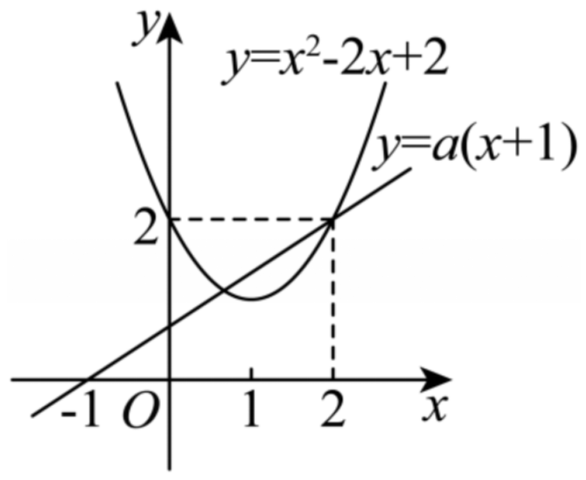
\includegraphics[width=0.30\textwidth]{figures/gao75_q12_graph.png}
\end{center}
% 原卷此处作“≥”，与题干严格不等号方向不一致，照录（见文件头“原卷笔误/存疑”①）
\step{由集合 $A$ 是“$2$ 集合”，故集合 $A$ 中只有一个元素，}
\step{得 $\begin{cases}2^2-2\times2+2\geqslant(2+1)a\\ 1^2-2\times1+2<(1+1)a\end{cases}$，解得 $\dfrac12<a\leqslant\dfrac23$，}
\step{故正实数 $a$ 的取值范围是 $\dfrac12<a\leqslant\dfrac23$.}
\solend
\fi

\end{enumerate}

\bigsec{二、选择题}

\begin{enumerate}
\setcounter{enumi}{12}

\item 已知全集 $U=\R$，集合 $A=\{x\mid x^2<4\}$，$B=\{y\mid y=x^2\}$，则图中阴影部分所表示的集合为\mbox{（\quad）}

\begin{center}
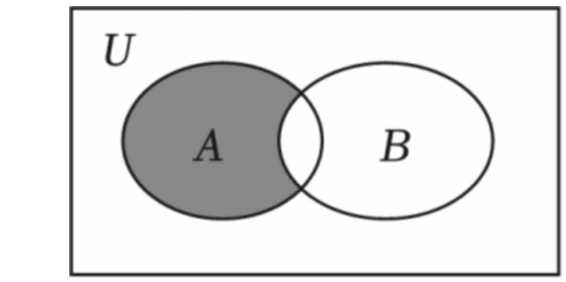
\includegraphics[width=0.26\textwidth]{figures/gao75_q13_venn.png}
\end{center}

\keepwithprev
A. $\{-2,-1,0\}$\qquad B. $(-\infty,4)$\qquad C. $(-2,0)$\qquad D. $(-2,0]$

\ifanswer
\solbegin
\step{集合 $A=\{x\mid x^2<4\}=(-2,2)$，$B=\{y\mid y=x^2\}=[0,+\infty)$，}
\step{图中阴影部分所表示的集合是 $A\cap\overline{B}=(-2,0)$. 故选 $C$.}
\solend
\fi

\item 已知 $x\in\R$，则“$\dfrac1x>1$”是“$x<1$”的\mbox{（\quad）}

\keepwithprev
A. 充分非必要条件\qquad B. 必要非充分条件\qquad C. 充要条件\qquad D. 既非充分又非必要条件

\ifanswer
\solbegin
\step{“$\dfrac1x>1$”$\Leftrightarrow0<x<1$，所以“$\dfrac1x>1$”是“$x<1$”的充分不必要条件. 故选 $A$.}
\solend
\fi

\item 已知集合 $M=\{x\mid x=m+\dfrac16,\,m\in\Z\}$，$N=\{x\mid x=\dfrac n2-\dfrac13,\,n\in\Z\}$，\\
$P=\{x\mid x=\dfrac p2+\dfrac16,\,p\in\Z\}$，则 $M$、$N$、$P$ 的关系为\mbox{（\quad）}

\keepwithprev
A. $M=N\subseteq P$\qquad B. $M\subseteq N=P$\qquad C. $M\subseteq N\subseteq P$\qquad D. $N\subseteq P\subseteq M$

\ifanswer
\solbegin
\step{集合 $N=\{x\mid x=\dfrac n2-\dfrac13,\,n\in\Z\}$，则 $x=\dfrac n2-\dfrac13=\dfrac{3n-2}6$，$n\in\Z$.}
\step{$P=\{x\mid x=\dfrac p2+\dfrac16,\,p\in\Z\}$，则 $x=\dfrac p2+\dfrac16=\dfrac{3p+1}6$，$p\in\Z$.}
\step{$M=\{x\mid x=m+\dfrac16,\,m\in\Z\}$，则 $x=m+\dfrac16=\dfrac{6m+1}6$，$m\in\Z$.}
\step{$M$、$N$、$P$ 三者分母相同，所以只需要比较他们的分子.}
\step{$M$：$6$ 的倍数$+1$，$N=P$：$3$ 的倍数$+1$，所以 $M\subseteq N=P$. 故选 $B$.}
\solend
\fi

\item 设集合 $P_1=\{x\mid x^2+ax+1>0\}$，$P_2=\{x\mid x^2+ax+2>0\}$，$Q_1=\{x\mid x^2+x+b>0\}$，$Q_2=\{x\mid x^2+2x+b>0\}$ 其中 $a,b\in\R$，给出下列两个命题：命题 $q_1$：对任意的 $a$，$P_1$ 是 $P_2$ 的子集；命题 $q_2$：对任意的 $b$，$Q_1$ 不是 $Q_2$ 的子集. 下列说法正确的是\mbox{（\quad）}

\keepwithprev
A. 命题 $q_1$ 是真命题，命题 $q_2$ 是假命题\qquad B. 命题 $q_1$ 是假命题，命题 $q_2$ 是真命题

C. 命题 $q_1$、$q_2$ 都是真命题\qquad D. 命题 $q_1$、$q_2$ 都是假命题

\ifanswer
\solbegin
\step{对于集合 $P_1=\{x\mid x^2+ax+1>0\}$，$P_2=\{x\mid x^2+ax+2>0\}$，}
\step{当 $m\in P_1$，即 $m^2+am+1>0$，得 $m^2+am+2>0$，}
\step{即有 $m\in P_2$，得对任意 $a$，$P_1$ 是 $P_2$ 的子集，命题 $q_1$ 为真命题；}
\step{当 $b=5$ 时，$Q_1=\{x\mid x^2+x+5>0\}=\R$，$Q_2=\{x\mid x^2+2x+5>0\}=\R$，}
\step{得 $Q_1$ 是 $Q_2$ 的子集；}
\step{存在 $b$，使得 $Q_1$ 是 $Q_2$ 的子集，故命题 $q_2$ 是假命题.}
\step{故选 $A$.}
\solend
\fi

\end{enumerate}

\bigsec{三、解答题}

\begin{enumerate}
\setcounter{enumi}{16}

\item 设集合 $A=\{x\mid x^2-2x=0\}$，$B=\{x\mid x^2+2(a+1)x+a^2-1=0\}$.

（1）写出集合 $A$ 的所有子集；

（2）若 $A\cap B=B$，求实数 $a$ 的取值范围.

\ifanswer
\solbegin
\stepm{(1)}{由 $x^2-2x=0$，得 $x=2$ 或 $x=0$，所以 $A=\{0,2\}$，}
\step{故集合 $A$ 的所有子集为 $\varnothing$、$\{0\}$、$\{2\}$、$\{0,2\}$.}
\stepm{(2)}{因为 $A\cap B=B$，所以 $B\subseteq A$，}
\step{方程 $x^2+2(a+1)x+a^2-1=0$，$\Delta=4(a+1)^2-4(a^2-1)=8a+8$，}
\step{若 $\Delta<0$，即 $a<-1$，方程 $x^2+2(a+1)x+a^2-1=0$ 无解，}
\step{此时 $B=\varnothing$，满足题意；}
\step{若 $\Delta=0$，即 $a=-1$，由 $x^2+2(a+1)x+a^2-1=0$，即 $x^2=0$，}
\step{解得 $x=0$，此时 $B=\{0\}$，满足题意；}
\step{若 $\Delta>0$，即 $a>-1$，要使 $B\subseteq A$，}
\step{则方程 $x^2+2(a+1)x+a^2-1=0$ 的解集为 $\{0,2\}$，}
\step{则 $\begin{cases}2+0=-2(a+1)\\ 2\times0=a^2-1\end{cases}$，$a$ 不存在.}
\step{综上所述，$a\leqslant-1$，即实数 $a$ 的取值范围为 $\{a\mid a\leqslant-1\}$.}
\solend
\fi

\ansspace

\item 已知全集 $U=\R$，集合 $A=\left\{x\,\middle|\,\dfrac{x-1}{x-3}<0\right\}$，$B=\{x\mid|x-a|<2\}$.

（1）当 $a=1$ 时，试用区间表示集合 $A$、$B$；

（2）若 $A\cup B=B$，求实数 $a$ 的取值范围.

\ifanswer
\solbegin
\stepm{(1)}{不等式 $\dfrac{x-1}{x-3}<0$ 可化为 $(x-1)(x-3)<0$，解得 $1<x<3$，即 $A=(1,3)$，}
\step{当 $a=1$ 时，$|x-1|<2$，则 $-2<x-1<2$，解得 $-1<x<3$，}
\step{即 $B=(-1,3)$；}
\stepm{(2)}{由不等式 $|x-a|<2$ 得 $-2<x-a<2$，解得 $-2+a<x<2+a$，}
\step{即 $B=\{x\mid-2+a<x<2+a\}$，}
\step{因为 $A\cup B=B$，所以 $A\subseteq B$，则 $\begin{cases}-2+a\leqslant1\\ 2+a\geqslant3\end{cases}$，解得 $1\leqslant a\leqslant3$，}
\step{即实数 $a$ 的取值范围为 $[1,3]$.}
\solend
\fi

\ansspace

\item 法国数学家弗朗索瓦·韦达 1615 年在著作《论方程的识别与订正》中建立了方程根与系数的关系. 发现一元二次方程 $ax^2+bx+c=0$，$a\neq0$ 的根与系数有如下的关系：

$x_1+x_2=-\dfrac ba$，$x_1x_2=\dfrac ca$，此即为韦达定理. 韦达定理的逆定理仍成立：如果两个数 $x_1$，$x_2$ 满足 $x_1+x_2=-\dfrac ba$，$x_1x_2=\dfrac ca$，则这两个数 $x_1$、$x_2$ 是方程 $ax^2+bx+c=0$，$a\neq0$ 的两个根. 例如：$m+n=-3$，$mn=2$，则 $m$、$n$ 是方程 $x^2+3x+2=0$ 的两个根. 请根据上述材料解决以下问题.

（1）已知 $m$、$n$ 是两个不相等的实数，满足 $m^2-6m-5=0$，$n^2-6n-5=0$，求 $\dfrac1m+\dfrac1n$ 的值；

（2）已知实数 $x$、$y$ 满足 $x+y+xy=17$，$x^2y+xy^2=72$，求 $x^2+y^2$ 的值.

\ifanswer
\solbegin
\stepm{(1)}{由题意，不相等的实数 $m$、$n$ 满足 $m^2-6m-5=0$、$n^2-6n-5=0$，}
\step{因此 $m$、$n$ 是一元二次方程 $x^2-6x-5=0$ 的两个不等实根.}
\step{由韦达定理得 $m+n=6$，$mn=-5$，因此 $\dfrac1m+\dfrac1n=\dfrac{m+n}{mn}=\dfrac6{-5}=-\dfrac65$.}
\stepm{(2)}{令 $s=x+y$，$t=xy$，}
\step{因为 $x+y+xy=17$，$x^2y+xy^2=72$，}
\step{即 $x+y+xy=17$，$xy(x+y)=72$，将已知条件变形得 $\begin{cases}s+t=17\\ st=72\end{cases}$.}
\step{由韦达定理逆定理，$s$、$t$ 是一元二次方程 $z^2-17z+72=0$ 的两个实根，}
\step{解方程得 $z_1=8$，$z_2=9$，即有两组解 $\begin{cases}s=8\\ t=9\end{cases}$ 和 $\begin{cases}s=9\\ t=8\end{cases}$.}
\step{当 $\begin{cases}s=8\\ t=9\end{cases}$ 时，$x$、$y$ 是方程 $w^2-8w+9=0$ 的根，}
\step{判别式 $\Delta=8^2-4\times1\times9=64-36=28>0$，符合题意，}
\step{此时 $x^2+y^2=(x+y)^2-2xy=s^2-2t=8^2-2\times9=64-18=46$；}
\step{当 $\begin{cases}s=9\\ t=8\end{cases}$ 时，$x$、$y$ 是方程 $w^2-9w+8=0$ 的根，}
\step{判别式 $\Delta=9^2-4\times1\times8=81-32=49>0$，符合题意，}
\step{此时 $x^2+y^2=(x+y)^2-2xy=s^2-2t=9^2-2\times8=81-16=65$.}
\step{综上，$x^2+y^2$ 的值为 $46$ 或 $65$.}
\solend
\fi

\ansspace

\item 已知关于 $x$ 的不等式 $ax^2-(a+1)x+b<0$.

（1）若不等式的解集是 $\{x\mid1<x<5\}$，求 $a+b$ 的值；

（2）若 $b=-\dfrac12$ 且不等式的解集为 $\R$，求 $a$ 取值范围；

（3）若 $b=1$，讨论此不等式的解集.

\ifanswer
\solbegin
\stepm{(1)}{由题意得 $1$ 和 $5$ 是方程 $ax^2-(a+1)x+b=0$ 的两个根且 $a>0$，}
\step{所以 $1+5=\dfrac{a+1}a$，$1\times5=\dfrac ba$，解得 $a=\dfrac15$，$b=1$，所以 $a+b=\dfrac65$.}
\stepm{(2)}{若 $b=-\dfrac12$，则不等式为 $ax^2-(a+1)x-\dfrac12<0$，}
\step{当 $a\neq0$，则有 $\begin{cases}a<0\\ \Delta=(a+1)^2+2a<0\end{cases}$，解得 $-2-\sqrt3<a<-2+\sqrt3$；}
\step{当 $a=0$，不等式即为 $-x-\dfrac12<0$，则 $x>-\dfrac12$，不合题意；}
\step{所以 $a$ 的取值范围是 $(-2-\sqrt3,-2+\sqrt3)$.}
\stepm{(3)}{若 $b=1$，则不等式为 $ax^2-(a+1)x+1<0$，即 $(ax-1)(x-1)<0$.}
\step{当 $a\neq0$ 时，由 $ax^2-(a+1)x+1<0$ 得 $(ax-1)(x-1)<0$.}
\step{方程 $(ax-1)(x-1)=0$ 的根为 $x=\dfrac1a$ 或 $x=1$，}
\step{当 $0<a<1$ 时，$\dfrac1a>1$，则不等式的解集为 $\left(1,\dfrac1a\right)$；}
\step{当 $a<0$ 时，$\dfrac1a<1$，则不等式的解集为 $\left(-\infty,\dfrac1a\right)\cup(1,+\infty)$；}
\step{当 $a=1$ 时，不等式即为 $(x-1)^2<0$，则不等式的解集为 $\varnothing$；}
\step{当 $a>1$ 时，$\dfrac1a<1$，则不等式的解集为 $\left(\dfrac1a,1\right)$；}
\step{当 $a=0$ 时，不等式为 $-x+1<0$，则不等式的解集为 $(1,+\infty)$；}
\step{综上所述，当 $a<0$ 时，不等式的解集为 $\left(-\infty,\dfrac1a\right)\cup(1,+\infty)$；}
\step{当 $a=0$ 时，不等式的解集为 $(1,+\infty)$；}
\step{当 $0<a<1$ 时，不等式的解集为 $\left(1,\dfrac1a\right)$；}
\step{当 $a=1$ 时，不等式的解集为 $\varnothing$；}
\step{当 $a>1$ 时，不等式的解集为 $\left(\dfrac1a,1\right)$.}
\solend
\fi

\ansspace

\item 已知关于 $x$ 的不等式① $x^2+2cx+c>0$，② $x^2+cx+c^2-1>0$，其中 $c$ 是实数.

（1）若 $1$ 是不等式②的一个解，求实数 $c$ 的取值范围；

（2）证明：不等式①、②中至多有一个恒成立；

（3）当 $c=0$ 时，“$x$ 满足 $|mx^2-4x+3|>5$”的一个必要非充分条件是“$x$ 满足 $x^2+cx+c^2-1>0$，求实数 $m$ 的取值范围.

\ifanswer
\solbegin
\stepm{(1)}{因为 $1$ 是不等式②的一个解，所以 $1+c+c^2-1>0$，}
\step{即 $c(c+1)>0$，解得 $c>0$ 或 $c<-1$，}
\step{所以实数 $c$ 的取值范围为 $(-\infty,-1)\cup(0,+\infty)$.}
\stepm{(2)}{假设不等式①、②都恒成立，}
\step{不等式① $x^2+2cx+c>0$ 恒成立，所以 $4c^2-4c<0$，所以 $0<c<1$；}
\step{② $x^2+cx+c^2-1>0$ 恒成立，所以 $c^2-4(c^2-1)<0$，$c^2>\dfrac43$，}
\step{解得 $c>\dfrac{2\sqrt3}3$ 或 $c<-\dfrac{2\sqrt3}3$；}
\step{所以当不等式①、②都恒成立时，}
\step{不等式组 $\begin{cases}0<c<1\\ c\in\left(-\infty,-\dfrac{2\sqrt3}3\right)\cup\left(\dfrac{2\sqrt3}3,+\infty\right)\end{cases}$ 无解，}
\step{所以假设不成立，}
\step{所以不等式①、②中至多有一个恒成立.}
\stepm{(3)}{当 $c=0$ 时，由 $x^2+cx+c^2-1>0$ 得 $x^2-1>0$，}
\step{解集为 $(-\infty,-1)\cup(1,+\infty)$.}
\step{记集合 $A=\{x\mid|mx^2-4x+3|>5\}$，集合 $B=\{x\mid x<-1\text{ 或 }x>1\}$.}
\step{由“$x$ 满足 $|mx^2-4x+3|>5$”的一个必要非充分条件是}
\step{“$x$ 满足 $x^2+cx+c^2-1>0$”得 $A$ 是 $B$ 的真子集.}
\step{所以 $\overline{B}$ 是 $A$ 的真子集，即对任意 $x\in[-1,1]$，$|mx^2-4x+3|\leqslant5$ 恒成立.}
\step{当 $x=0$ 时，不等式 $-5\leqslant mx^2-4x+3\leqslant5$ 恒成立；}
\step{当 $x\in[-1,0)\cup(0,1]$ 时，}
\step{则 $mx^2-4x+3\geqslant-5$ 与 $mx^2-4x+3\leqslant5$ 同时成立.}
\step{①由 $mx^2-4x+3\geqslant-5$，得 $m\geqslant\dfrac{4x-8}{x^2}$，求值域得 $\dfrac{4x-8}{x^2}$ 的最大值 $=-4$，}
\step{所以 $m\geqslant-4$.}
\step{②由 $mx^2-4x+3\leqslant5$，得 $m\leqslant\dfrac{4x+2}{x^2}$，求值域得 $\dfrac{4x+2}{x^2}$ 的最小值 $=-2$，}
\step{所以 $m\leqslant-2$.}
\step{综上所述，实数 $m$ 的取值范围为 $[-4,-2]$.}
\solend
\fi

\ansspace*[7]

\end{enumerate}

\end{document}
"
% 紧凑版：xelatex "\def\iscompact{1}% 高一75_市二中学_10月月考.tex
%   —— 高一上数学“2026-2027 年市二中学高一上 10 月月考”（讲评版）
% 试卷版：xelatex 高一75_市二中学_10月月考.tex
% 答案版：xelatex "\def\isanswer{1}% 高一75_市二中学_10月月考.tex
%   —— 高一上数学“2026-2027 年市二中学高一上 10 月月考”（讲评版）
% 试卷版：xelatex 高一75_市二中学_10月月考.tex
% 答案版：xelatex "\def\isanswer{1}\input{高一75_市二中学_10月月考.tex}"
% 紧凑版：xelatex "\def\iscompact{1}\input{高一75_市二中学_10月月考.tex}"
%
% 原始材料：微信公众号“魔都数学加油站”文章，连载“27学年高一75”；
% 原文标题“27学年高一75——2026-2027年上海市市二中学高一上10月月考”；
% 原文链接：https://mp.weixin.qq.com/s/dhxtwWEZgKLxeKdkbWqOhw。
% 页面标注发布时间 2026-10-22 21:45（上海）。
% 正文为 11 张 PNG 页（`原图/高一75_市二中学_10月月考/01..11.png`）：
% 第 2、4、5、6、9 页为 4762×6735，其余 6 页为 2560×3620，均按页序读取。
% 11 页全为试卷正文页（卷首标题在第 1 页页顶，卷末第 21 题 (3) 解析止于第 11 页），
% 无封面页、目录页、二维码或宣传页。粉色斜排“魔都数学加油站”为卷面水印，未录入。
%
% 卷首标题：照卷面印作“2026-2027 年市二中学高一上 10 月月考”（黑体加粗一行）。
% 原卷年份区间用半角连字符，本稿按全稿惯例排 en dash；原卷无副标题。
%
% 篇幅与题号：原卷自第 3 题起编号（第 1、2 题不在本卷内）。填空题 3—12（10 题）、
% 选择题 13—16（4 题）、解答题 17—21（5 题），共 19 题。本稿沿用原节与原题号，
% 只改排为全稿统一的大节样式。
%
% 讲评版：原卷第 4 题只印【答案】（“$[-1,2]$”），本稿只给 \ans{}；其余 18 题均印
% 【解析】，用 \solbegin…\solend。四道选择题的作答括号原卷即留空，答案写在解析末句
% “故选 C／A／B／A”，照录在解析内，不另提 \ans{}。
%
% 副标题：原卷未印副标题。本稿按“知识模块”口径标作“集合与常用逻辑用语、不等式”：
% 19 题中集合与常用逻辑用语 9 题（第 3、4、5、8、10、12、13、15、17、18 题中的集合题），
% 不等式 10 题（第 6、7、9、11、19、20、21 题及第 12、20 题的不等式部分），两类均确有
% 分量，故并标。口径同 高一63、高一68—74。
%
% 与原卷的排版差异：
%   ① 原卷每题下直接印【答案】/【解析】，本稿按全稿惯例将答案与解析置于答案版；
%   ② 原卷未印副标题，本稿按“知识模块”口径补出；
%   ③ 原卷填空横线约四个字宽，本稿按全稿惯例统一排 \blankline[4.4em]；
%   ④ 原卷数集记号排粗体 $\mathbf{R}$（第 5、6、7、9、10、14、18、20、21 题），本稿
%      按全稿惯例改用 $\R$（同 高一68—74）；第 11 题的“解集为 $\R$”同此；
%   ⑤ 原卷句末标点多为西文句点，均逐处照录；
%   ⑥ 第 17—21 题的子问原卷印作“（1）…（2）…”，本稿按 高一69—74 成例用行内
%      “（1）（2）（3）”段，解析中的子问标号用 \stepm{(1)}{…}；
%   ⑦ 每道解答题原卷未留作答空白，本稿按全稿惯例加 \ansspace（末题用 \ansspace*）；
%   ⑧ 选择题的作答括号原卷排半角“(    )”，本稿按全稿惯例排 \mbox{（\quad）}；
%      选项行排照原卷——第 13、14 题一行四条，第 15、16 题一行四条；
%   ⑨ 第 9、12、15、17—21 题解析中的不等式组／方程组，原卷均排作“{”连接的多行式，
%      本稿按全稿惯例排 cases；
%   ⑩ 第 12 题解析有一幅“抛物线 + 直线”图：原卷印在解析第 3 行右侧、题干无“如图”二字
%      （解析里写“两函数图象如图：”）。本稿按原卷截图裁取（`figures/gao75_q12_graph.png`，
%      由第 3 页原图裁出、去除粉色水印后转灰度，未放大），放在答案版解析第 3 条之后；
%   ⑪ 第 13 题题干中间有一幅韦恩图（全集矩形内含 A、B 两圆，A 涂灰）：原卷印在题干
%      右侧、题干句子被图隔开。本稿按原卷截图裁取（`figures/gao75_q13_venn.png`，由第 3
%      页原图裁出、去除粉色水印后转灰度，并抹去左侧侵入的“分”字），放在题干之后、
%      选项之前，仅答案版出。
%
% 原卷笔误/存疑（均照录未改，正文对应处另有 % 注）：
%   ① 第 12 题解析列不等式组时写 $2^2-2\times2+2\geqslant(2+1)a$，与
%      $x^2-2x+2<a(x+1)$ 的严格不等号方向不一致；原卷如此，照录未改。
%   ② 第 14 题选项 A—D 的“充分非必要”“必要非充分”“既非充分又非必要”与原卷
%      其它题的“充分不必要”写法不同，照录未统一。
%   ④ 第 21 题 (3) 题干的“$x$ 满足 $|mx^2-4x+3|>5$”的一个必要非充分条件是
%      “$x$ 满足 $x^2+cx+c^2-1>0$，原卷只有左引号、无右引号（且逗号在引号内），
%      本稿照录未补。
%   ③ 第 20 题 (2) 的解集写成 $(-2-\sqrt3,-2+\sqrt3)$，其中 $a<0$ 与 $\Delta<0$ 联立后
%      左端点应为 $-2-\sqrt3$、右端点为 $-2+\sqrt3$；原卷如此，照录未改。
%
% 行数核对：逐题数 \step/\stepm 条数与原卷【解析】印刷行数，18 题逐一相符，
% 合计 132 条 / 132 行（Q3：6；Q5：1；Q6：2；Q7：1；Q8：2；Q9：3；Q10：10；
% Q11：8；Q12：6；Q13：2；Q14：1；Q15：5；Q16：7；Q17：12；Q18：7；Q19：15；
% Q20：19；Q21：25）。另第 4 题只印【答案】，提 \ans{}，不计入 \step 账。
%
% 插图：第 12 题解析的抛物线图、第 13 题题干的韦恩图，见上⑩⑪；其余题干无配图。
%
\documentclass[a4paper,11pt]{article}
\usepackage{common}

\begin{document}

\examtitlest[3]{2026--2027 年市二中学高一上 10 月月考}{集合与常用逻辑用语、不等式}

\bigsec{一、填空题}

\begin{enumerate}
\setcounter{enumi}{2}

\item 已知集合 $A=\{a,a^2\}$，且 $1\in A$，则 $a=$\blankline[4.4em].

\ifanswer
\solbegin
\step{因为 $1\in A=\{a,a^2\}$，所以 $a=1$ 或 $a^2=1$.}
\step{又集合 $A=\{a,a^2\}$ 是用列举法写出两个元素的，其元素必须互异，故 $a\neq a^2$，}
\step{即 $a\neq0$ 且 $a\neq1$，所以 $a=1$ 应舍去；}
\step{由 $a^2=1$ 得 $a=1$（舍去）或 $a=-1$.}
\step{当 $a=-1$ 时，$A=\{-1,1\}$，满足 $1\in A$ 且两个元素互异.}
\step{故 $a=-1$.}
\solend
\fi

\item 已知集合 $A=[-1,1]$，$B=[0,2]$，则 $A\cup B=$\blankline[4.4em].

\ifanswer
\ans{$[-1,2]$}
\fi

\item 已知全集 $U=\R$，集合 $A=\{x\mid x\neq1\}$，则 $\overline{A}=$\blankline[4.4em].

\ifanswer
\solbegin
\step{因为全集 $U=\R$，集合 $A=\{x\mid x\neq1\}$，所以 $\overline{A}=\{x\mid x=1\}$.}
\solend
\fi

\item 设 $x\in\R$，不等式 $x^2-4x<0$ 的解集用区间表示是\blankline[4.4em].

\ifanswer
\solbegin
\step{因为 $x^2-4x<0$，即 $x(x-4)<0$，所以 $0<x<4$，}
\step{所以 $x(x-4)<0$ 的解集为 $(0,4)$.}
\solend
\fi

\item 已知 $m\in\R$，若关于 $x$ 的方程 $2mx^2+3x+m-1=m^2\cdot x^2+(m+1)x+1$ 解集为 $\R$，则 $m$ 的值为\blankline[4.4em].

\ifanswer
\solbegin
\step{由题意得 $2m=m^2$，$3=m+1$，$m-1=1$，所以 $m=2$.}
\solend
\fi

\item 设 $\alpha:x\leqslant m$，$\beta:|x-2|\leqslant1$，若 $\alpha$ 是 $\beta$ 的必要条件，则实数 $m$ 的取值范围是\blankline[4.4em].

\ifanswer
\solbegin
\step{由 $|x-2|\leqslant1$，得 $-1\leqslant x-2\leqslant1$，解得 $1\leqslant x\leqslant3$，}
\step{因为 $\alpha$ 是 $\beta$ 的必要条件，所以 $\{x\mid1\leqslant x\leqslant3\}\subseteq\{x\mid x\leqslant m\}$，得 $m\geqslant3$.}
\solend
\fi

\item 设 $a\in\R$，若关于 $x$ 的不等式 $\dfrac{a}{x-1}\leqslant1$ 的解集是 $(-\infty,1)\cup[2,+\infty)$，则 $a$ 的值为\blankline[4.4em].

\ifanswer
\solbegin
\step{不等式可变形为 $\dfrac{a+1-x}{x-1}\leqslant0$，等价于 $\begin{cases}(a+1-x)(x-1)\leqslant0\\ x-1\neq0\end{cases}$，}
\step{因为原不等式的解集是 $(-\infty,1)\cup[2,+\infty)$，}
\step{所以 $1$，$2$ 是方程 $(a+1-x)(x-1)=0$ 的两根，所以 $a+1=2$，解得 $a=1$.}
\solend
\fi

\item 下列命题：① “$x>1$ 或 $y>1$”的否定形式是“$x\leqslant1$ 或 $y\leqslant1$”，② 若 $A\cup B=B$，则 $A\subseteq B$，③ 方程 $ax+1=0$ 的解是 $x=-\frac1a$，④ “$ac=bc$”是“$a=b$”的必要非充分条件，⑤ “任意 $x\in\R$，$f(x)=f(-x)$”的否定形式是“存在 $x_0\in\R$，使得 $f(x_0)\neq f(-x_0)$”其中真命题的序号是\blankline[4.4em]（填写序号）.

\ifanswer
\solbegin
\step{①假命题：“$x>1$ 或 $y>1$”的否定形式是“$x\leqslant1$ 且 $y\leqslant1$”；}
\step{②真命题：$A\cup B=B\Leftrightarrow A\subseteq B$；}
\step{③假命题：当 $a=0$ 时，方程无解，因此该命题忽略了 $a=0$ 的情况；}
\step{④真命题：先判断必要性：若 $a=b$，则有 $ac=bc$，所以必要性成立；}
\step{再判断充分性：若 $ac=bc$，即 $(a-b)c=0$，当 $c=0$ 时，$a$ 和 $b$ 可以不相等，}
\step{因此充分性不成立.}
\step{⑤真命题：全称命题的否定是存在量词命题，}
\step{“任意 $x\in\R$，$f(x)=f(-x)$”的否定形式是}
\step{“存在 $x_0\in\R$，使得 $f(x_0)\neq f(-x_0)$”，表述正确.}
\step{故正确的是②④⑤.}
\solend
\fi

\item 为了加强家校联系，蔡老师组建了一个由学生、家长和教师组成的微信群. 已知该群中男学生人数多于女学生人数，女学生人数多于家长人数，家长人数多于教师人数，教师人数的两倍多于男学生人数. 则该微信群人数的最小值为\blankline[4.4em].

\ifanswer
\solbegin
\step{设男学生、女学生、家长、教师的人数分别为 $M$、$F$、$P$、$T$，}
\step{它们都是正整数.}
\step{由题意得 $M>F>P>T$，且教师人数的两倍多于男学生人数，即 $2T>M$.}
\step{由 $M>F>P>T$ 得 $M\geqslant T+3$；}
\step{又 $2T>M\geqslant T+3$，所以 $2T>T+3$，解得 $T>3$，故教师人数最少为 $T=4$.}
\step{当 $T=4$ 时，为使总人数最少，取 $P=5$、$F=6$、$M=7$，}
\step{此时 $7>6>5>4$ 且 $2\times4=8>7$，满足题意.}
\step{于是微信群人数为 $4+5+6+7=22$，所以该微信群人数的最小值为 $22$.}
\solend
\fi

\item 若集合 $M$ 有 $k$ 个子集，则称集合 $M$ 为“$k$ 集合”，\\
已知集合 $A=\{x\mid x^2-(a+2)x+2-a<0,\,x\in\Z\}$ 是“$2$ 集合”，则正实数 $a$ 的取值范围是\blankline[4.4em].

\ifanswer
\solbegin
\step{由 $x^2-(a+2)x+2-a<0$，得 $x^2-2x+2<a(x+1)$，}
\step{设二次函数 $y=x^2-2x+2$ 与一次函数 $y=a(x+1)$，}
\needvspace{13\baselineskip}
\step{由 $a>0$，$y=a(x+1)$ 过定点 $(-1,0)$，两函数图象如图：}
\begin{center}
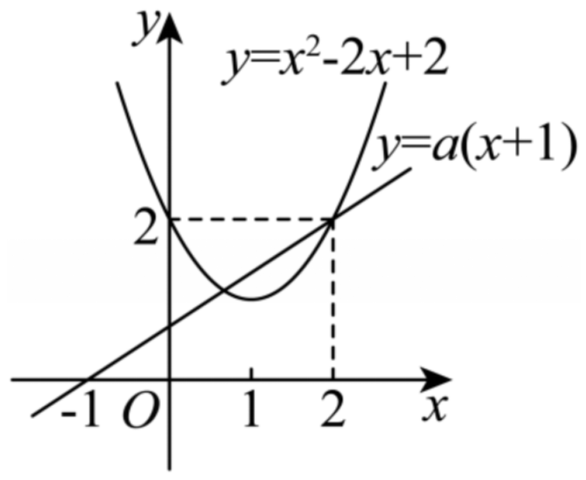
\includegraphics[width=0.30\textwidth]{figures/gao75_q12_graph.png}
\end{center}
% 原卷此处作“≥”，与题干严格不等号方向不一致，照录（见文件头“原卷笔误/存疑”①）
\step{由集合 $A$ 是“$2$ 集合”，故集合 $A$ 中只有一个元素，}
\step{得 $\begin{cases}2^2-2\times2+2\geqslant(2+1)a\\ 1^2-2\times1+2<(1+1)a\end{cases}$，解得 $\dfrac12<a\leqslant\dfrac23$，}
\step{故正实数 $a$ 的取值范围是 $\dfrac12<a\leqslant\dfrac23$.}
\solend
\fi

\end{enumerate}

\bigsec{二、选择题}

\begin{enumerate}
\setcounter{enumi}{12}

\item 已知全集 $U=\R$，集合 $A=\{x\mid x^2<4\}$，$B=\{y\mid y=x^2\}$，则图中阴影部分所表示的集合为\mbox{（\quad）}

\begin{center}
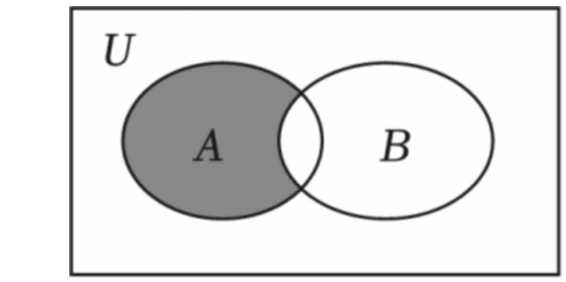
\includegraphics[width=0.26\textwidth]{figures/gao75_q13_venn.png}
\end{center}

\keepwithprev
A. $\{-2,-1,0\}$\qquad B. $(-\infty,4)$\qquad C. $(-2,0)$\qquad D. $(-2,0]$

\ifanswer
\solbegin
\step{集合 $A=\{x\mid x^2<4\}=(-2,2)$，$B=\{y\mid y=x^2\}=[0,+\infty)$，}
\step{图中阴影部分所表示的集合是 $A\cap\overline{B}=(-2,0)$. 故选 $C$.}
\solend
\fi

\item 已知 $x\in\R$，则“$\dfrac1x>1$”是“$x<1$”的\mbox{（\quad）}

\keepwithprev
A. 充分非必要条件\qquad B. 必要非充分条件\qquad C. 充要条件\qquad D. 既非充分又非必要条件

\ifanswer
\solbegin
\step{“$\dfrac1x>1$”$\Leftrightarrow0<x<1$，所以“$\dfrac1x>1$”是“$x<1$”的充分不必要条件. 故选 $A$.}
\solend
\fi

\item 已知集合 $M=\{x\mid x=m+\dfrac16,\,m\in\Z\}$，$N=\{x\mid x=\dfrac n2-\dfrac13,\,n\in\Z\}$，\\
$P=\{x\mid x=\dfrac p2+\dfrac16,\,p\in\Z\}$，则 $M$、$N$、$P$ 的关系为\mbox{（\quad）}

\keepwithprev
A. $M=N\subseteq P$\qquad B. $M\subseteq N=P$\qquad C. $M\subseteq N\subseteq P$\qquad D. $N\subseteq P\subseteq M$

\ifanswer
\solbegin
\step{集合 $N=\{x\mid x=\dfrac n2-\dfrac13,\,n\in\Z\}$，则 $x=\dfrac n2-\dfrac13=\dfrac{3n-2}6$，$n\in\Z$.}
\step{$P=\{x\mid x=\dfrac p2+\dfrac16,\,p\in\Z\}$，则 $x=\dfrac p2+\dfrac16=\dfrac{3p+1}6$，$p\in\Z$.}
\step{$M=\{x\mid x=m+\dfrac16,\,m\in\Z\}$，则 $x=m+\dfrac16=\dfrac{6m+1}6$，$m\in\Z$.}
\step{$M$、$N$、$P$ 三者分母相同，所以只需要比较他们的分子.}
\step{$M$：$6$ 的倍数$+1$，$N=P$：$3$ 的倍数$+1$，所以 $M\subseteq N=P$. 故选 $B$.}
\solend
\fi

\item 设集合 $P_1=\{x\mid x^2+ax+1>0\}$，$P_2=\{x\mid x^2+ax+2>0\}$，$Q_1=\{x\mid x^2+x+b>0\}$，$Q_2=\{x\mid x^2+2x+b>0\}$ 其中 $a,b\in\R$，给出下列两个命题：命题 $q_1$：对任意的 $a$，$P_1$ 是 $P_2$ 的子集；命题 $q_2$：对任意的 $b$，$Q_1$ 不是 $Q_2$ 的子集. 下列说法正确的是\mbox{（\quad）}

\keepwithprev
A. 命题 $q_1$ 是真命题，命题 $q_2$ 是假命题\qquad B. 命题 $q_1$ 是假命题，命题 $q_2$ 是真命题

C. 命题 $q_1$、$q_2$ 都是真命题\qquad D. 命题 $q_1$、$q_2$ 都是假命题

\ifanswer
\solbegin
\step{对于集合 $P_1=\{x\mid x^2+ax+1>0\}$，$P_2=\{x\mid x^2+ax+2>0\}$，}
\step{当 $m\in P_1$，即 $m^2+am+1>0$，得 $m^2+am+2>0$，}
\step{即有 $m\in P_2$，得对任意 $a$，$P_1$ 是 $P_2$ 的子集，命题 $q_1$ 为真命题；}
\step{当 $b=5$ 时，$Q_1=\{x\mid x^2+x+5>0\}=\R$，$Q_2=\{x\mid x^2+2x+5>0\}=\R$，}
\step{得 $Q_1$ 是 $Q_2$ 的子集；}
\step{存在 $b$，使得 $Q_1$ 是 $Q_2$ 的子集，故命题 $q_2$ 是假命题.}
\step{故选 $A$.}
\solend
\fi

\end{enumerate}

\bigsec{三、解答题}

\begin{enumerate}
\setcounter{enumi}{16}

\item 设集合 $A=\{x\mid x^2-2x=0\}$，$B=\{x\mid x^2+2(a+1)x+a^2-1=0\}$.

（1）写出集合 $A$ 的所有子集；

（2）若 $A\cap B=B$，求实数 $a$ 的取值范围.

\ifanswer
\solbegin
\stepm{(1)}{由 $x^2-2x=0$，得 $x=2$ 或 $x=0$，所以 $A=\{0,2\}$，}
\step{故集合 $A$ 的所有子集为 $\varnothing$、$\{0\}$、$\{2\}$、$\{0,2\}$.}
\stepm{(2)}{因为 $A\cap B=B$，所以 $B\subseteq A$，}
\step{方程 $x^2+2(a+1)x+a^2-1=0$，$\Delta=4(a+1)^2-4(a^2-1)=8a+8$，}
\step{若 $\Delta<0$，即 $a<-1$，方程 $x^2+2(a+1)x+a^2-1=0$ 无解，}
\step{此时 $B=\varnothing$，满足题意；}
\step{若 $\Delta=0$，即 $a=-1$，由 $x^2+2(a+1)x+a^2-1=0$，即 $x^2=0$，}
\step{解得 $x=0$，此时 $B=\{0\}$，满足题意；}
\step{若 $\Delta>0$，即 $a>-1$，要使 $B\subseteq A$，}
\step{则方程 $x^2+2(a+1)x+a^2-1=0$ 的解集为 $\{0,2\}$，}
\step{则 $\begin{cases}2+0=-2(a+1)\\ 2\times0=a^2-1\end{cases}$，$a$ 不存在.}
\step{综上所述，$a\leqslant-1$，即实数 $a$ 的取值范围为 $\{a\mid a\leqslant-1\}$.}
\solend
\fi

\ansspace

\item 已知全集 $U=\R$，集合 $A=\left\{x\,\middle|\,\dfrac{x-1}{x-3}<0\right\}$，$B=\{x\mid|x-a|<2\}$.

（1）当 $a=1$ 时，试用区间表示集合 $A$、$B$；

（2）若 $A\cup B=B$，求实数 $a$ 的取值范围.

\ifanswer
\solbegin
\stepm{(1)}{不等式 $\dfrac{x-1}{x-3}<0$ 可化为 $(x-1)(x-3)<0$，解得 $1<x<3$，即 $A=(1,3)$，}
\step{当 $a=1$ 时，$|x-1|<2$，则 $-2<x-1<2$，解得 $-1<x<3$，}
\step{即 $B=(-1,3)$；}
\stepm{(2)}{由不等式 $|x-a|<2$ 得 $-2<x-a<2$，解得 $-2+a<x<2+a$，}
\step{即 $B=\{x\mid-2+a<x<2+a\}$，}
\step{因为 $A\cup B=B$，所以 $A\subseteq B$，则 $\begin{cases}-2+a\leqslant1\\ 2+a\geqslant3\end{cases}$，解得 $1\leqslant a\leqslant3$，}
\step{即实数 $a$ 的取值范围为 $[1,3]$.}
\solend
\fi

\ansspace

\item 法国数学家弗朗索瓦·韦达 1615 年在著作《论方程的识别与订正》中建立了方程根与系数的关系. 发现一元二次方程 $ax^2+bx+c=0$，$a\neq0$ 的根与系数有如下的关系：

$x_1+x_2=-\dfrac ba$，$x_1x_2=\dfrac ca$，此即为韦达定理. 韦达定理的逆定理仍成立：如果两个数 $x_1$，$x_2$ 满足 $x_1+x_2=-\dfrac ba$，$x_1x_2=\dfrac ca$，则这两个数 $x_1$、$x_2$ 是方程 $ax^2+bx+c=0$，$a\neq0$ 的两个根. 例如：$m+n=-3$，$mn=2$，则 $m$、$n$ 是方程 $x^2+3x+2=0$ 的两个根. 请根据上述材料解决以下问题.

（1）已知 $m$、$n$ 是两个不相等的实数，满足 $m^2-6m-5=0$，$n^2-6n-5=0$，求 $\dfrac1m+\dfrac1n$ 的值；

（2）已知实数 $x$、$y$ 满足 $x+y+xy=17$，$x^2y+xy^2=72$，求 $x^2+y^2$ 的值.

\ifanswer
\solbegin
\stepm{(1)}{由题意，不相等的实数 $m$、$n$ 满足 $m^2-6m-5=0$、$n^2-6n-5=0$，}
\step{因此 $m$、$n$ 是一元二次方程 $x^2-6x-5=0$ 的两个不等实根.}
\step{由韦达定理得 $m+n=6$，$mn=-5$，因此 $\dfrac1m+\dfrac1n=\dfrac{m+n}{mn}=\dfrac6{-5}=-\dfrac65$.}
\stepm{(2)}{令 $s=x+y$，$t=xy$，}
\step{因为 $x+y+xy=17$，$x^2y+xy^2=72$，}
\step{即 $x+y+xy=17$，$xy(x+y)=72$，将已知条件变形得 $\begin{cases}s+t=17\\ st=72\end{cases}$.}
\step{由韦达定理逆定理，$s$、$t$ 是一元二次方程 $z^2-17z+72=0$ 的两个实根，}
\step{解方程得 $z_1=8$，$z_2=9$，即有两组解 $\begin{cases}s=8\\ t=9\end{cases}$ 和 $\begin{cases}s=9\\ t=8\end{cases}$.}
\step{当 $\begin{cases}s=8\\ t=9\end{cases}$ 时，$x$、$y$ 是方程 $w^2-8w+9=0$ 的根，}
\step{判别式 $\Delta=8^2-4\times1\times9=64-36=28>0$，符合题意，}
\step{此时 $x^2+y^2=(x+y)^2-2xy=s^2-2t=8^2-2\times9=64-18=46$；}
\step{当 $\begin{cases}s=9\\ t=8\end{cases}$ 时，$x$、$y$ 是方程 $w^2-9w+8=0$ 的根，}
\step{判别式 $\Delta=9^2-4\times1\times8=81-32=49>0$，符合题意，}
\step{此时 $x^2+y^2=(x+y)^2-2xy=s^2-2t=9^2-2\times8=81-16=65$.}
\step{综上，$x^2+y^2$ 的值为 $46$ 或 $65$.}
\solend
\fi

\ansspace

\item 已知关于 $x$ 的不等式 $ax^2-(a+1)x+b<0$.

（1）若不等式的解集是 $\{x\mid1<x<5\}$，求 $a+b$ 的值；

（2）若 $b=-\dfrac12$ 且不等式的解集为 $\R$，求 $a$ 取值范围；

（3）若 $b=1$，讨论此不等式的解集.

\ifanswer
\solbegin
\stepm{(1)}{由题意得 $1$ 和 $5$ 是方程 $ax^2-(a+1)x+b=0$ 的两个根且 $a>0$，}
\step{所以 $1+5=\dfrac{a+1}a$，$1\times5=\dfrac ba$，解得 $a=\dfrac15$，$b=1$，所以 $a+b=\dfrac65$.}
\stepm{(2)}{若 $b=-\dfrac12$，则不等式为 $ax^2-(a+1)x-\dfrac12<0$，}
\step{当 $a\neq0$，则有 $\begin{cases}a<0\\ \Delta=(a+1)^2+2a<0\end{cases}$，解得 $-2-\sqrt3<a<-2+\sqrt3$；}
\step{当 $a=0$，不等式即为 $-x-\dfrac12<0$，则 $x>-\dfrac12$，不合题意；}
\step{所以 $a$ 的取值范围是 $(-2-\sqrt3,-2+\sqrt3)$.}
\stepm{(3)}{若 $b=1$，则不等式为 $ax^2-(a+1)x+1<0$，即 $(ax-1)(x-1)<0$.}
\step{当 $a\neq0$ 时，由 $ax^2-(a+1)x+1<0$ 得 $(ax-1)(x-1)<0$.}
\step{方程 $(ax-1)(x-1)=0$ 的根为 $x=\dfrac1a$ 或 $x=1$，}
\step{当 $0<a<1$ 时，$\dfrac1a>1$，则不等式的解集为 $\left(1,\dfrac1a\right)$；}
\step{当 $a<0$ 时，$\dfrac1a<1$，则不等式的解集为 $\left(-\infty,\dfrac1a\right)\cup(1,+\infty)$；}
\step{当 $a=1$ 时，不等式即为 $(x-1)^2<0$，则不等式的解集为 $\varnothing$；}
\step{当 $a>1$ 时，$\dfrac1a<1$，则不等式的解集为 $\left(\dfrac1a,1\right)$；}
\step{当 $a=0$ 时，不等式为 $-x+1<0$，则不等式的解集为 $(1,+\infty)$；}
\step{综上所述，当 $a<0$ 时，不等式的解集为 $\left(-\infty,\dfrac1a\right)\cup(1,+\infty)$；}
\step{当 $a=0$ 时，不等式的解集为 $(1,+\infty)$；}
\step{当 $0<a<1$ 时，不等式的解集为 $\left(1,\dfrac1a\right)$；}
\step{当 $a=1$ 时，不等式的解集为 $\varnothing$；}
\step{当 $a>1$ 时，不等式的解集为 $\left(\dfrac1a,1\right)$.}
\solend
\fi

\ansspace

\item 已知关于 $x$ 的不等式① $x^2+2cx+c>0$，② $x^2+cx+c^2-1>0$，其中 $c$ 是实数.

（1）若 $1$ 是不等式②的一个解，求实数 $c$ 的取值范围；

（2）证明：不等式①、②中至多有一个恒成立；

（3）当 $c=0$ 时，“$x$ 满足 $|mx^2-4x+3|>5$”的一个必要非充分条件是“$x$ 满足 $x^2+cx+c^2-1>0$，求实数 $m$ 的取值范围.

\ifanswer
\solbegin
\stepm{(1)}{因为 $1$ 是不等式②的一个解，所以 $1+c+c^2-1>0$，}
\step{即 $c(c+1)>0$，解得 $c>0$ 或 $c<-1$，}
\step{所以实数 $c$ 的取值范围为 $(-\infty,-1)\cup(0,+\infty)$.}
\stepm{(2)}{假设不等式①、②都恒成立，}
\step{不等式① $x^2+2cx+c>0$ 恒成立，所以 $4c^2-4c<0$，所以 $0<c<1$；}
\step{② $x^2+cx+c^2-1>0$ 恒成立，所以 $c^2-4(c^2-1)<0$，$c^2>\dfrac43$，}
\step{解得 $c>\dfrac{2\sqrt3}3$ 或 $c<-\dfrac{2\sqrt3}3$；}
\step{所以当不等式①、②都恒成立时，}
\step{不等式组 $\begin{cases}0<c<1\\ c\in\left(-\infty,-\dfrac{2\sqrt3}3\right)\cup\left(\dfrac{2\sqrt3}3,+\infty\right)\end{cases}$ 无解，}
\step{所以假设不成立，}
\step{所以不等式①、②中至多有一个恒成立.}
\stepm{(3)}{当 $c=0$ 时，由 $x^2+cx+c^2-1>0$ 得 $x^2-1>0$，}
\step{解集为 $(-\infty,-1)\cup(1,+\infty)$.}
\step{记集合 $A=\{x\mid|mx^2-4x+3|>5\}$，集合 $B=\{x\mid x<-1\text{ 或 }x>1\}$.}
\step{由“$x$ 满足 $|mx^2-4x+3|>5$”的一个必要非充分条件是}
\step{“$x$ 满足 $x^2+cx+c^2-1>0$”得 $A$ 是 $B$ 的真子集.}
\step{所以 $\overline{B}$ 是 $A$ 的真子集，即对任意 $x\in[-1,1]$，$|mx^2-4x+3|\leqslant5$ 恒成立.}
\step{当 $x=0$ 时，不等式 $-5\leqslant mx^2-4x+3\leqslant5$ 恒成立；}
\step{当 $x\in[-1,0)\cup(0,1]$ 时，}
\step{则 $mx^2-4x+3\geqslant-5$ 与 $mx^2-4x+3\leqslant5$ 同时成立.}
\step{①由 $mx^2-4x+3\geqslant-5$，得 $m\geqslant\dfrac{4x-8}{x^2}$，求值域得 $\dfrac{4x-8}{x^2}$ 的最大值 $=-4$，}
\step{所以 $m\geqslant-4$.}
\step{②由 $mx^2-4x+3\leqslant5$，得 $m\leqslant\dfrac{4x+2}{x^2}$，求值域得 $\dfrac{4x+2}{x^2}$ 的最小值 $=-2$，}
\step{所以 $m\leqslant-2$.}
\step{综上所述，实数 $m$ 的取值范围为 $[-4,-2]$.}
\solend
\fi

\ansspace*[7]

\end{enumerate}

\end{document}
"
% 紧凑版：xelatex "\def\iscompact{1}% 高一75_市二中学_10月月考.tex
%   —— 高一上数学“2026-2027 年市二中学高一上 10 月月考”（讲评版）
% 试卷版：xelatex 高一75_市二中学_10月月考.tex
% 答案版：xelatex "\def\isanswer{1}\input{高一75_市二中学_10月月考.tex}"
% 紧凑版：xelatex "\def\iscompact{1}\input{高一75_市二中学_10月月考.tex}"
%
% 原始材料：微信公众号“魔都数学加油站”文章，连载“27学年高一75”；
% 原文标题“27学年高一75——2026-2027年上海市市二中学高一上10月月考”；
% 原文链接：https://mp.weixin.qq.com/s/dhxtwWEZgKLxeKdkbWqOhw。
% 页面标注发布时间 2026-10-22 21:45（上海）。
% 正文为 11 张 PNG 页（`原图/高一75_市二中学_10月月考/01..11.png`）：
% 第 2、4、5、6、9 页为 4762×6735，其余 6 页为 2560×3620，均按页序读取。
% 11 页全为试卷正文页（卷首标题在第 1 页页顶，卷末第 21 题 (3) 解析止于第 11 页），
% 无封面页、目录页、二维码或宣传页。粉色斜排“魔都数学加油站”为卷面水印，未录入。
%
% 卷首标题：照卷面印作“2026-2027 年市二中学高一上 10 月月考”（黑体加粗一行）。
% 原卷年份区间用半角连字符，本稿按全稿惯例排 en dash；原卷无副标题。
%
% 篇幅与题号：原卷自第 3 题起编号（第 1、2 题不在本卷内）。填空题 3—12（10 题）、
% 选择题 13—16（4 题）、解答题 17—21（5 题），共 19 题。本稿沿用原节与原题号，
% 只改排为全稿统一的大节样式。
%
% 讲评版：原卷第 4 题只印【答案】（“$[-1,2]$”），本稿只给 \ans{}；其余 18 题均印
% 【解析】，用 \solbegin…\solend。四道选择题的作答括号原卷即留空，答案写在解析末句
% “故选 C／A／B／A”，照录在解析内，不另提 \ans{}。
%
% 副标题：原卷未印副标题。本稿按“知识模块”口径标作“集合与常用逻辑用语、不等式”：
% 19 题中集合与常用逻辑用语 9 题（第 3、4、5、8、10、12、13、15、17、18 题中的集合题），
% 不等式 10 题（第 6、7、9、11、19、20、21 题及第 12、20 题的不等式部分），两类均确有
% 分量，故并标。口径同 高一63、高一68—74。
%
% 与原卷的排版差异：
%   ① 原卷每题下直接印【答案】/【解析】，本稿按全稿惯例将答案与解析置于答案版；
%   ② 原卷未印副标题，本稿按“知识模块”口径补出；
%   ③ 原卷填空横线约四个字宽，本稿按全稿惯例统一排 \blankline[4.4em]；
%   ④ 原卷数集记号排粗体 $\mathbf{R}$（第 5、6、7、9、10、14、18、20、21 题），本稿
%      按全稿惯例改用 $\R$（同 高一68—74）；第 11 题的“解集为 $\R$”同此；
%   ⑤ 原卷句末标点多为西文句点，均逐处照录；
%   ⑥ 第 17—21 题的子问原卷印作“（1）…（2）…”，本稿按 高一69—74 成例用行内
%      “（1）（2）（3）”段，解析中的子问标号用 \stepm{(1)}{…}；
%   ⑦ 每道解答题原卷未留作答空白，本稿按全稿惯例加 \ansspace（末题用 \ansspace*）；
%   ⑧ 选择题的作答括号原卷排半角“(    )”，本稿按全稿惯例排 \mbox{（\quad）}；
%      选项行排照原卷——第 13、14 题一行四条，第 15、16 题一行四条；
%   ⑨ 第 9、12、15、17—21 题解析中的不等式组／方程组，原卷均排作“{”连接的多行式，
%      本稿按全稿惯例排 cases；
%   ⑩ 第 12 题解析有一幅“抛物线 + 直线”图：原卷印在解析第 3 行右侧、题干无“如图”二字
%      （解析里写“两函数图象如图：”）。本稿按原卷截图裁取（`figures/gao75_q12_graph.png`，
%      由第 3 页原图裁出、去除粉色水印后转灰度，未放大），放在答案版解析第 3 条之后；
%   ⑪ 第 13 题题干中间有一幅韦恩图（全集矩形内含 A、B 两圆，A 涂灰）：原卷印在题干
%      右侧、题干句子被图隔开。本稿按原卷截图裁取（`figures/gao75_q13_venn.png`，由第 3
%      页原图裁出、去除粉色水印后转灰度，并抹去左侧侵入的“分”字），放在题干之后、
%      选项之前，仅答案版出。
%
% 原卷笔误/存疑（均照录未改，正文对应处另有 % 注）：
%   ① 第 12 题解析列不等式组时写 $2^2-2\times2+2\geqslant(2+1)a$，与
%      $x^2-2x+2<a(x+1)$ 的严格不等号方向不一致；原卷如此，照录未改。
%   ② 第 14 题选项 A—D 的“充分非必要”“必要非充分”“既非充分又非必要”与原卷
%      其它题的“充分不必要”写法不同，照录未统一。
%   ④ 第 21 题 (3) 题干的“$x$ 满足 $|mx^2-4x+3|>5$”的一个必要非充分条件是
%      “$x$ 满足 $x^2+cx+c^2-1>0$，原卷只有左引号、无右引号（且逗号在引号内），
%      本稿照录未补。
%   ③ 第 20 题 (2) 的解集写成 $(-2-\sqrt3,-2+\sqrt3)$，其中 $a<0$ 与 $\Delta<0$ 联立后
%      左端点应为 $-2-\sqrt3$、右端点为 $-2+\sqrt3$；原卷如此，照录未改。
%
% 行数核对：逐题数 \step/\stepm 条数与原卷【解析】印刷行数，18 题逐一相符，
% 合计 132 条 / 132 行（Q3：6；Q5：1；Q6：2；Q7：1；Q8：2；Q9：3；Q10：10；
% Q11：8；Q12：6；Q13：2；Q14：1；Q15：5；Q16：7；Q17：12；Q18：7；Q19：15；
% Q20：19；Q21：25）。另第 4 题只印【答案】，提 \ans{}，不计入 \step 账。
%
% 插图：第 12 题解析的抛物线图、第 13 题题干的韦恩图，见上⑩⑪；其余题干无配图。
%
\documentclass[a4paper,11pt]{article}
\usepackage{common}

\begin{document}

\examtitlest[3]{2026--2027 年市二中学高一上 10 月月考}{集合与常用逻辑用语、不等式}

\bigsec{一、填空题}

\begin{enumerate}
\setcounter{enumi}{2}

\item 已知集合 $A=\{a,a^2\}$，且 $1\in A$，则 $a=$\blankline[4.4em].

\ifanswer
\solbegin
\step{因为 $1\in A=\{a,a^2\}$，所以 $a=1$ 或 $a^2=1$.}
\step{又集合 $A=\{a,a^2\}$ 是用列举法写出两个元素的，其元素必须互异，故 $a\neq a^2$，}
\step{即 $a\neq0$ 且 $a\neq1$，所以 $a=1$ 应舍去；}
\step{由 $a^2=1$ 得 $a=1$（舍去）或 $a=-1$.}
\step{当 $a=-1$ 时，$A=\{-1,1\}$，满足 $1\in A$ 且两个元素互异.}
\step{故 $a=-1$.}
\solend
\fi

\item 已知集合 $A=[-1,1]$，$B=[0,2]$，则 $A\cup B=$\blankline[4.4em].

\ifanswer
\ans{$[-1,2]$}
\fi

\item 已知全集 $U=\R$，集合 $A=\{x\mid x\neq1\}$，则 $\overline{A}=$\blankline[4.4em].

\ifanswer
\solbegin
\step{因为全集 $U=\R$，集合 $A=\{x\mid x\neq1\}$，所以 $\overline{A}=\{x\mid x=1\}$.}
\solend
\fi

\item 设 $x\in\R$，不等式 $x^2-4x<0$ 的解集用区间表示是\blankline[4.4em].

\ifanswer
\solbegin
\step{因为 $x^2-4x<0$，即 $x(x-4)<0$，所以 $0<x<4$，}
\step{所以 $x(x-4)<0$ 的解集为 $(0,4)$.}
\solend
\fi

\item 已知 $m\in\R$，若关于 $x$ 的方程 $2mx^2+3x+m-1=m^2\cdot x^2+(m+1)x+1$ 解集为 $\R$，则 $m$ 的值为\blankline[4.4em].

\ifanswer
\solbegin
\step{由题意得 $2m=m^2$，$3=m+1$，$m-1=1$，所以 $m=2$.}
\solend
\fi

\item 设 $\alpha:x\leqslant m$，$\beta:|x-2|\leqslant1$，若 $\alpha$ 是 $\beta$ 的必要条件，则实数 $m$ 的取值范围是\blankline[4.4em].

\ifanswer
\solbegin
\step{由 $|x-2|\leqslant1$，得 $-1\leqslant x-2\leqslant1$，解得 $1\leqslant x\leqslant3$，}
\step{因为 $\alpha$ 是 $\beta$ 的必要条件，所以 $\{x\mid1\leqslant x\leqslant3\}\subseteq\{x\mid x\leqslant m\}$，得 $m\geqslant3$.}
\solend
\fi

\item 设 $a\in\R$，若关于 $x$ 的不等式 $\dfrac{a}{x-1}\leqslant1$ 的解集是 $(-\infty,1)\cup[2,+\infty)$，则 $a$ 的值为\blankline[4.4em].

\ifanswer
\solbegin
\step{不等式可变形为 $\dfrac{a+1-x}{x-1}\leqslant0$，等价于 $\begin{cases}(a+1-x)(x-1)\leqslant0\\ x-1\neq0\end{cases}$，}
\step{因为原不等式的解集是 $(-\infty,1)\cup[2,+\infty)$，}
\step{所以 $1$，$2$ 是方程 $(a+1-x)(x-1)=0$ 的两根，所以 $a+1=2$，解得 $a=1$.}
\solend
\fi

\item 下列命题：① “$x>1$ 或 $y>1$”的否定形式是“$x\leqslant1$ 或 $y\leqslant1$”，② 若 $A\cup B=B$，则 $A\subseteq B$，③ 方程 $ax+1=0$ 的解是 $x=-\frac1a$，④ “$ac=bc$”是“$a=b$”的必要非充分条件，⑤ “任意 $x\in\R$，$f(x)=f(-x)$”的否定形式是“存在 $x_0\in\R$，使得 $f(x_0)\neq f(-x_0)$”其中真命题的序号是\blankline[4.4em]（填写序号）.

\ifanswer
\solbegin
\step{①假命题：“$x>1$ 或 $y>1$”的否定形式是“$x\leqslant1$ 且 $y\leqslant1$”；}
\step{②真命题：$A\cup B=B\Leftrightarrow A\subseteq B$；}
\step{③假命题：当 $a=0$ 时，方程无解，因此该命题忽略了 $a=0$ 的情况；}
\step{④真命题：先判断必要性：若 $a=b$，则有 $ac=bc$，所以必要性成立；}
\step{再判断充分性：若 $ac=bc$，即 $(a-b)c=0$，当 $c=0$ 时，$a$ 和 $b$ 可以不相等，}
\step{因此充分性不成立.}
\step{⑤真命题：全称命题的否定是存在量词命题，}
\step{“任意 $x\in\R$，$f(x)=f(-x)$”的否定形式是}
\step{“存在 $x_0\in\R$，使得 $f(x_0)\neq f(-x_0)$”，表述正确.}
\step{故正确的是②④⑤.}
\solend
\fi

\item 为了加强家校联系，蔡老师组建了一个由学生、家长和教师组成的微信群. 已知该群中男学生人数多于女学生人数，女学生人数多于家长人数，家长人数多于教师人数，教师人数的两倍多于男学生人数. 则该微信群人数的最小值为\blankline[4.4em].

\ifanswer
\solbegin
\step{设男学生、女学生、家长、教师的人数分别为 $M$、$F$、$P$、$T$，}
\step{它们都是正整数.}
\step{由题意得 $M>F>P>T$，且教师人数的两倍多于男学生人数，即 $2T>M$.}
\step{由 $M>F>P>T$ 得 $M\geqslant T+3$；}
\step{又 $2T>M\geqslant T+3$，所以 $2T>T+3$，解得 $T>3$，故教师人数最少为 $T=4$.}
\step{当 $T=4$ 时，为使总人数最少，取 $P=5$、$F=6$、$M=7$，}
\step{此时 $7>6>5>4$ 且 $2\times4=8>7$，满足题意.}
\step{于是微信群人数为 $4+5+6+7=22$，所以该微信群人数的最小值为 $22$.}
\solend
\fi

\item 若集合 $M$ 有 $k$ 个子集，则称集合 $M$ 为“$k$ 集合”，\\
已知集合 $A=\{x\mid x^2-(a+2)x+2-a<0,\,x\in\Z\}$ 是“$2$ 集合”，则正实数 $a$ 的取值范围是\blankline[4.4em].

\ifanswer
\solbegin
\step{由 $x^2-(a+2)x+2-a<0$，得 $x^2-2x+2<a(x+1)$，}
\step{设二次函数 $y=x^2-2x+2$ 与一次函数 $y=a(x+1)$，}
\needvspace{13\baselineskip}
\step{由 $a>0$，$y=a(x+1)$ 过定点 $(-1,0)$，两函数图象如图：}
\begin{center}
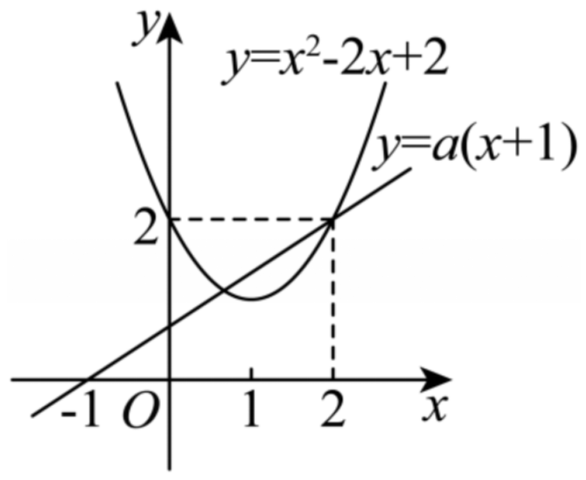
\includegraphics[width=0.30\textwidth]{figures/gao75_q12_graph.png}
\end{center}
% 原卷此处作“≥”，与题干严格不等号方向不一致，照录（见文件头“原卷笔误/存疑”①）
\step{由集合 $A$ 是“$2$ 集合”，故集合 $A$ 中只有一个元素，}
\step{得 $\begin{cases}2^2-2\times2+2\geqslant(2+1)a\\ 1^2-2\times1+2<(1+1)a\end{cases}$，解得 $\dfrac12<a\leqslant\dfrac23$，}
\step{故正实数 $a$ 的取值范围是 $\dfrac12<a\leqslant\dfrac23$.}
\solend
\fi

\end{enumerate}

\bigsec{二、选择题}

\begin{enumerate}
\setcounter{enumi}{12}

\item 已知全集 $U=\R$，集合 $A=\{x\mid x^2<4\}$，$B=\{y\mid y=x^2\}$，则图中阴影部分所表示的集合为\mbox{（\quad）}

\begin{center}
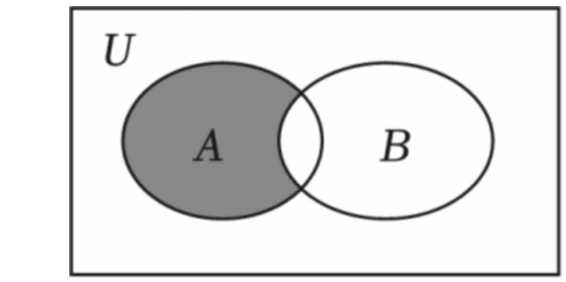
\includegraphics[width=0.26\textwidth]{figures/gao75_q13_venn.png}
\end{center}

\keepwithprev
A. $\{-2,-1,0\}$\qquad B. $(-\infty,4)$\qquad C. $(-2,0)$\qquad D. $(-2,0]$

\ifanswer
\solbegin
\step{集合 $A=\{x\mid x^2<4\}=(-2,2)$，$B=\{y\mid y=x^2\}=[0,+\infty)$，}
\step{图中阴影部分所表示的集合是 $A\cap\overline{B}=(-2,0)$. 故选 $C$.}
\solend
\fi

\item 已知 $x\in\R$，则“$\dfrac1x>1$”是“$x<1$”的\mbox{（\quad）}

\keepwithprev
A. 充分非必要条件\qquad B. 必要非充分条件\qquad C. 充要条件\qquad D. 既非充分又非必要条件

\ifanswer
\solbegin
\step{“$\dfrac1x>1$”$\Leftrightarrow0<x<1$，所以“$\dfrac1x>1$”是“$x<1$”的充分不必要条件. 故选 $A$.}
\solend
\fi

\item 已知集合 $M=\{x\mid x=m+\dfrac16,\,m\in\Z\}$，$N=\{x\mid x=\dfrac n2-\dfrac13,\,n\in\Z\}$，\\
$P=\{x\mid x=\dfrac p2+\dfrac16,\,p\in\Z\}$，则 $M$、$N$、$P$ 的关系为\mbox{（\quad）}

\keepwithprev
A. $M=N\subseteq P$\qquad B. $M\subseteq N=P$\qquad C. $M\subseteq N\subseteq P$\qquad D. $N\subseteq P\subseteq M$

\ifanswer
\solbegin
\step{集合 $N=\{x\mid x=\dfrac n2-\dfrac13,\,n\in\Z\}$，则 $x=\dfrac n2-\dfrac13=\dfrac{3n-2}6$，$n\in\Z$.}
\step{$P=\{x\mid x=\dfrac p2+\dfrac16,\,p\in\Z\}$，则 $x=\dfrac p2+\dfrac16=\dfrac{3p+1}6$，$p\in\Z$.}
\step{$M=\{x\mid x=m+\dfrac16,\,m\in\Z\}$，则 $x=m+\dfrac16=\dfrac{6m+1}6$，$m\in\Z$.}
\step{$M$、$N$、$P$ 三者分母相同，所以只需要比较他们的分子.}
\step{$M$：$6$ 的倍数$+1$，$N=P$：$3$ 的倍数$+1$，所以 $M\subseteq N=P$. 故选 $B$.}
\solend
\fi

\item 设集合 $P_1=\{x\mid x^2+ax+1>0\}$，$P_2=\{x\mid x^2+ax+2>0\}$，$Q_1=\{x\mid x^2+x+b>0\}$，$Q_2=\{x\mid x^2+2x+b>0\}$ 其中 $a,b\in\R$，给出下列两个命题：命题 $q_1$：对任意的 $a$，$P_1$ 是 $P_2$ 的子集；命题 $q_2$：对任意的 $b$，$Q_1$ 不是 $Q_2$ 的子集. 下列说法正确的是\mbox{（\quad）}

\keepwithprev
A. 命题 $q_1$ 是真命题，命题 $q_2$ 是假命题\qquad B. 命题 $q_1$ 是假命题，命题 $q_2$ 是真命题

C. 命题 $q_1$、$q_2$ 都是真命题\qquad D. 命题 $q_1$、$q_2$ 都是假命题

\ifanswer
\solbegin
\step{对于集合 $P_1=\{x\mid x^2+ax+1>0\}$，$P_2=\{x\mid x^2+ax+2>0\}$，}
\step{当 $m\in P_1$，即 $m^2+am+1>0$，得 $m^2+am+2>0$，}
\step{即有 $m\in P_2$，得对任意 $a$，$P_1$ 是 $P_2$ 的子集，命题 $q_1$ 为真命题；}
\step{当 $b=5$ 时，$Q_1=\{x\mid x^2+x+5>0\}=\R$，$Q_2=\{x\mid x^2+2x+5>0\}=\R$，}
\step{得 $Q_1$ 是 $Q_2$ 的子集；}
\step{存在 $b$，使得 $Q_1$ 是 $Q_2$ 的子集，故命题 $q_2$ 是假命题.}
\step{故选 $A$.}
\solend
\fi

\end{enumerate}

\bigsec{三、解答题}

\begin{enumerate}
\setcounter{enumi}{16}

\item 设集合 $A=\{x\mid x^2-2x=0\}$，$B=\{x\mid x^2+2(a+1)x+a^2-1=0\}$.

（1）写出集合 $A$ 的所有子集；

（2）若 $A\cap B=B$，求实数 $a$ 的取值范围.

\ifanswer
\solbegin
\stepm{(1)}{由 $x^2-2x=0$，得 $x=2$ 或 $x=0$，所以 $A=\{0,2\}$，}
\step{故集合 $A$ 的所有子集为 $\varnothing$、$\{0\}$、$\{2\}$、$\{0,2\}$.}
\stepm{(2)}{因为 $A\cap B=B$，所以 $B\subseteq A$，}
\step{方程 $x^2+2(a+1)x+a^2-1=0$，$\Delta=4(a+1)^2-4(a^2-1)=8a+8$，}
\step{若 $\Delta<0$，即 $a<-1$，方程 $x^2+2(a+1)x+a^2-1=0$ 无解，}
\step{此时 $B=\varnothing$，满足题意；}
\step{若 $\Delta=0$，即 $a=-1$，由 $x^2+2(a+1)x+a^2-1=0$，即 $x^2=0$，}
\step{解得 $x=0$，此时 $B=\{0\}$，满足题意；}
\step{若 $\Delta>0$，即 $a>-1$，要使 $B\subseteq A$，}
\step{则方程 $x^2+2(a+1)x+a^2-1=0$ 的解集为 $\{0,2\}$，}
\step{则 $\begin{cases}2+0=-2(a+1)\\ 2\times0=a^2-1\end{cases}$，$a$ 不存在.}
\step{综上所述，$a\leqslant-1$，即实数 $a$ 的取值范围为 $\{a\mid a\leqslant-1\}$.}
\solend
\fi

\ansspace

\item 已知全集 $U=\R$，集合 $A=\left\{x\,\middle|\,\dfrac{x-1}{x-3}<0\right\}$，$B=\{x\mid|x-a|<2\}$.

（1）当 $a=1$ 时，试用区间表示集合 $A$、$B$；

（2）若 $A\cup B=B$，求实数 $a$ 的取值范围.

\ifanswer
\solbegin
\stepm{(1)}{不等式 $\dfrac{x-1}{x-3}<0$ 可化为 $(x-1)(x-3)<0$，解得 $1<x<3$，即 $A=(1,3)$，}
\step{当 $a=1$ 时，$|x-1|<2$，则 $-2<x-1<2$，解得 $-1<x<3$，}
\step{即 $B=(-1,3)$；}
\stepm{(2)}{由不等式 $|x-a|<2$ 得 $-2<x-a<2$，解得 $-2+a<x<2+a$，}
\step{即 $B=\{x\mid-2+a<x<2+a\}$，}
\step{因为 $A\cup B=B$，所以 $A\subseteq B$，则 $\begin{cases}-2+a\leqslant1\\ 2+a\geqslant3\end{cases}$，解得 $1\leqslant a\leqslant3$，}
\step{即实数 $a$ 的取值范围为 $[1,3]$.}
\solend
\fi

\ansspace

\item 法国数学家弗朗索瓦·韦达 1615 年在著作《论方程的识别与订正》中建立了方程根与系数的关系. 发现一元二次方程 $ax^2+bx+c=0$，$a\neq0$ 的根与系数有如下的关系：

$x_1+x_2=-\dfrac ba$，$x_1x_2=\dfrac ca$，此即为韦达定理. 韦达定理的逆定理仍成立：如果两个数 $x_1$，$x_2$ 满足 $x_1+x_2=-\dfrac ba$，$x_1x_2=\dfrac ca$，则这两个数 $x_1$、$x_2$ 是方程 $ax^2+bx+c=0$，$a\neq0$ 的两个根. 例如：$m+n=-3$，$mn=2$，则 $m$、$n$ 是方程 $x^2+3x+2=0$ 的两个根. 请根据上述材料解决以下问题.

（1）已知 $m$、$n$ 是两个不相等的实数，满足 $m^2-6m-5=0$，$n^2-6n-5=0$，求 $\dfrac1m+\dfrac1n$ 的值；

（2）已知实数 $x$、$y$ 满足 $x+y+xy=17$，$x^2y+xy^2=72$，求 $x^2+y^2$ 的值.

\ifanswer
\solbegin
\stepm{(1)}{由题意，不相等的实数 $m$、$n$ 满足 $m^2-6m-5=0$、$n^2-6n-5=0$，}
\step{因此 $m$、$n$ 是一元二次方程 $x^2-6x-5=0$ 的两个不等实根.}
\step{由韦达定理得 $m+n=6$，$mn=-5$，因此 $\dfrac1m+\dfrac1n=\dfrac{m+n}{mn}=\dfrac6{-5}=-\dfrac65$.}
\stepm{(2)}{令 $s=x+y$，$t=xy$，}
\step{因为 $x+y+xy=17$，$x^2y+xy^2=72$，}
\step{即 $x+y+xy=17$，$xy(x+y)=72$，将已知条件变形得 $\begin{cases}s+t=17\\ st=72\end{cases}$.}
\step{由韦达定理逆定理，$s$、$t$ 是一元二次方程 $z^2-17z+72=0$ 的两个实根，}
\step{解方程得 $z_1=8$，$z_2=9$，即有两组解 $\begin{cases}s=8\\ t=9\end{cases}$ 和 $\begin{cases}s=9\\ t=8\end{cases}$.}
\step{当 $\begin{cases}s=8\\ t=9\end{cases}$ 时，$x$、$y$ 是方程 $w^2-8w+9=0$ 的根，}
\step{判别式 $\Delta=8^2-4\times1\times9=64-36=28>0$，符合题意，}
\step{此时 $x^2+y^2=(x+y)^2-2xy=s^2-2t=8^2-2\times9=64-18=46$；}
\step{当 $\begin{cases}s=9\\ t=8\end{cases}$ 时，$x$、$y$ 是方程 $w^2-9w+8=0$ 的根，}
\step{判别式 $\Delta=9^2-4\times1\times8=81-32=49>0$，符合题意，}
\step{此时 $x^2+y^2=(x+y)^2-2xy=s^2-2t=9^2-2\times8=81-16=65$.}
\step{综上，$x^2+y^2$ 的值为 $46$ 或 $65$.}
\solend
\fi

\ansspace

\item 已知关于 $x$ 的不等式 $ax^2-(a+1)x+b<0$.

（1）若不等式的解集是 $\{x\mid1<x<5\}$，求 $a+b$ 的值；

（2）若 $b=-\dfrac12$ 且不等式的解集为 $\R$，求 $a$ 取值范围；

（3）若 $b=1$，讨论此不等式的解集.

\ifanswer
\solbegin
\stepm{(1)}{由题意得 $1$ 和 $5$ 是方程 $ax^2-(a+1)x+b=0$ 的两个根且 $a>0$，}
\step{所以 $1+5=\dfrac{a+1}a$，$1\times5=\dfrac ba$，解得 $a=\dfrac15$，$b=1$，所以 $a+b=\dfrac65$.}
\stepm{(2)}{若 $b=-\dfrac12$，则不等式为 $ax^2-(a+1)x-\dfrac12<0$，}
\step{当 $a\neq0$，则有 $\begin{cases}a<0\\ \Delta=(a+1)^2+2a<0\end{cases}$，解得 $-2-\sqrt3<a<-2+\sqrt3$；}
\step{当 $a=0$，不等式即为 $-x-\dfrac12<0$，则 $x>-\dfrac12$，不合题意；}
\step{所以 $a$ 的取值范围是 $(-2-\sqrt3,-2+\sqrt3)$.}
\stepm{(3)}{若 $b=1$，则不等式为 $ax^2-(a+1)x+1<0$，即 $(ax-1)(x-1)<0$.}
\step{当 $a\neq0$ 时，由 $ax^2-(a+1)x+1<0$ 得 $(ax-1)(x-1)<0$.}
\step{方程 $(ax-1)(x-1)=0$ 的根为 $x=\dfrac1a$ 或 $x=1$，}
\step{当 $0<a<1$ 时，$\dfrac1a>1$，则不等式的解集为 $\left(1,\dfrac1a\right)$；}
\step{当 $a<0$ 时，$\dfrac1a<1$，则不等式的解集为 $\left(-\infty,\dfrac1a\right)\cup(1,+\infty)$；}
\step{当 $a=1$ 时，不等式即为 $(x-1)^2<0$，则不等式的解集为 $\varnothing$；}
\step{当 $a>1$ 时，$\dfrac1a<1$，则不等式的解集为 $\left(\dfrac1a,1\right)$；}
\step{当 $a=0$ 时，不等式为 $-x+1<0$，则不等式的解集为 $(1,+\infty)$；}
\step{综上所述，当 $a<0$ 时，不等式的解集为 $\left(-\infty,\dfrac1a\right)\cup(1,+\infty)$；}
\step{当 $a=0$ 时，不等式的解集为 $(1,+\infty)$；}
\step{当 $0<a<1$ 时，不等式的解集为 $\left(1,\dfrac1a\right)$；}
\step{当 $a=1$ 时，不等式的解集为 $\varnothing$；}
\step{当 $a>1$ 时，不等式的解集为 $\left(\dfrac1a,1\right)$.}
\solend
\fi

\ansspace

\item 已知关于 $x$ 的不等式① $x^2+2cx+c>0$，② $x^2+cx+c^2-1>0$，其中 $c$ 是实数.

（1）若 $1$ 是不等式②的一个解，求实数 $c$ 的取值范围；

（2）证明：不等式①、②中至多有一个恒成立；

（3）当 $c=0$ 时，“$x$ 满足 $|mx^2-4x+3|>5$”的一个必要非充分条件是“$x$ 满足 $x^2+cx+c^2-1>0$，求实数 $m$ 的取值范围.

\ifanswer
\solbegin
\stepm{(1)}{因为 $1$ 是不等式②的一个解，所以 $1+c+c^2-1>0$，}
\step{即 $c(c+1)>0$，解得 $c>0$ 或 $c<-1$，}
\step{所以实数 $c$ 的取值范围为 $(-\infty,-1)\cup(0,+\infty)$.}
\stepm{(2)}{假设不等式①、②都恒成立，}
\step{不等式① $x^2+2cx+c>0$ 恒成立，所以 $4c^2-4c<0$，所以 $0<c<1$；}
\step{② $x^2+cx+c^2-1>0$ 恒成立，所以 $c^2-4(c^2-1)<0$，$c^2>\dfrac43$，}
\step{解得 $c>\dfrac{2\sqrt3}3$ 或 $c<-\dfrac{2\sqrt3}3$；}
\step{所以当不等式①、②都恒成立时，}
\step{不等式组 $\begin{cases}0<c<1\\ c\in\left(-\infty,-\dfrac{2\sqrt3}3\right)\cup\left(\dfrac{2\sqrt3}3,+\infty\right)\end{cases}$ 无解，}
\step{所以假设不成立，}
\step{所以不等式①、②中至多有一个恒成立.}
\stepm{(3)}{当 $c=0$ 时，由 $x^2+cx+c^2-1>0$ 得 $x^2-1>0$，}
\step{解集为 $(-\infty,-1)\cup(1,+\infty)$.}
\step{记集合 $A=\{x\mid|mx^2-4x+3|>5\}$，集合 $B=\{x\mid x<-1\text{ 或 }x>1\}$.}
\step{由“$x$ 满足 $|mx^2-4x+3|>5$”的一个必要非充分条件是}
\step{“$x$ 满足 $x^2+cx+c^2-1>0$”得 $A$ 是 $B$ 的真子集.}
\step{所以 $\overline{B}$ 是 $A$ 的真子集，即对任意 $x\in[-1,1]$，$|mx^2-4x+3|\leqslant5$ 恒成立.}
\step{当 $x=0$ 时，不等式 $-5\leqslant mx^2-4x+3\leqslant5$ 恒成立；}
\step{当 $x\in[-1,0)\cup(0,1]$ 时，}
\step{则 $mx^2-4x+3\geqslant-5$ 与 $mx^2-4x+3\leqslant5$ 同时成立.}
\step{①由 $mx^2-4x+3\geqslant-5$，得 $m\geqslant\dfrac{4x-8}{x^2}$，求值域得 $\dfrac{4x-8}{x^2}$ 的最大值 $=-4$，}
\step{所以 $m\geqslant-4$.}
\step{②由 $mx^2-4x+3\leqslant5$，得 $m\leqslant\dfrac{4x+2}{x^2}$，求值域得 $\dfrac{4x+2}{x^2}$ 的最小值 $=-2$，}
\step{所以 $m\leqslant-2$.}
\step{综上所述，实数 $m$ 的取值范围为 $[-4,-2]$.}
\solend
\fi

\ansspace*[7]

\end{enumerate}

\end{document}
"
%
% 原始材料：微信公众号“魔都数学加油站”文章，连载“27学年高一75”；
% 原文标题“27学年高一75——2026-2027年上海市市二中学高一上10月月考”；
% 原文链接：https://mp.weixin.qq.com/s/dhxtwWEZgKLxeKdkbWqOhw。
% 页面标注发布时间 2026-10-22 21:45（上海）。
% 正文为 11 张 PNG 页（`原图/高一75_市二中学_10月月考/01..11.png`）：
% 第 2、4、5、6、9 页为 4762×6735，其余 6 页为 2560×3620，均按页序读取。
% 11 页全为试卷正文页（卷首标题在第 1 页页顶，卷末第 21 题 (3) 解析止于第 11 页），
% 无封面页、目录页、二维码或宣传页。粉色斜排“魔都数学加油站”为卷面水印，未录入。
%
% 卷首标题：照卷面印作“2026-2027 年市二中学高一上 10 月月考”（黑体加粗一行）。
% 原卷年份区间用半角连字符，本稿按全稿惯例排 en dash；原卷无副标题。
%
% 篇幅与题号：原卷自第 3 题起编号（第 1、2 题不在本卷内）。填空题 3—12（10 题）、
% 选择题 13—16（4 题）、解答题 17—21（5 题），共 19 题。本稿沿用原节与原题号，
% 只改排为全稿统一的大节样式。
%
% 讲评版：原卷第 4 题只印【答案】（“$[-1,2]$”），本稿只给 \ans{}；其余 18 题均印
% 【解析】，用 \solbegin…\solend。四道选择题的作答括号原卷即留空，答案写在解析末句
% “故选 C／A／B／A”，照录在解析内，不另提 \ans{}。
%
% 副标题：原卷未印副标题。本稿按“知识模块”口径标作“集合与常用逻辑用语、不等式”：
% 19 题中集合与常用逻辑用语 9 题（第 3、4、5、8、10、12、13、15、17、18 题中的集合题），
% 不等式 10 题（第 6、7、9、11、19、20、21 题及第 12、20 题的不等式部分），两类均确有
% 分量，故并标。口径同 高一63、高一68—74。
%
% 与原卷的排版差异：
%   ① 原卷每题下直接印【答案】/【解析】，本稿按全稿惯例将答案与解析置于答案版；
%   ② 原卷未印副标题，本稿按“知识模块”口径补出；
%   ③ 原卷填空横线约四个字宽，本稿按全稿惯例统一排 \blankline[4.4em]；
%   ④ 原卷数集记号排粗体 $\mathbf{R}$（第 5、6、7、9、10、14、18、20、21 题），本稿
%      按全稿惯例改用 $\R$（同 高一68—74）；第 11 题的“解集为 $\R$”同此；
%   ⑤ 原卷句末标点多为西文句点，均逐处照录；
%   ⑥ 第 17—21 题的子问原卷印作“（1）…（2）…”，本稿按 高一69—74 成例用行内
%      “（1）（2）（3）”段，解析中的子问标号用 \stepm{(1)}{…}；
%   ⑦ 每道解答题原卷未留作答空白，本稿按全稿惯例加 \ansspace（末题用 \ansspace*）；
%   ⑧ 选择题的作答括号原卷排半角“(    )”，本稿按全稿惯例排 \mbox{（\quad）}；
%      选项行排照原卷——第 13、14 题一行四条，第 15、16 题一行四条；
%   ⑨ 第 9、12、15、17—21 题解析中的不等式组／方程组，原卷均排作“{”连接的多行式，
%      本稿按全稿惯例排 cases；
%   ⑩ 第 12 题解析有一幅“抛物线 + 直线”图：原卷印在解析第 3 行右侧、题干无“如图”二字
%      （解析里写“两函数图象如图：”）。本稿按原卷截图裁取（`figures/gao75_q12_graph.png`，
%      由第 3 页原图裁出、去除粉色水印后转灰度，未放大），放在答案版解析第 3 条之后；
%   ⑪ 第 13 题题干中间有一幅韦恩图（全集矩形内含 A、B 两圆，A 涂灰）：原卷印在题干
%      右侧、题干句子被图隔开。本稿按原卷截图裁取（`figures/gao75_q13_venn.png`，由第 3
%      页原图裁出、去除粉色水印后转灰度，并抹去左侧侵入的“分”字），放在题干之后、
%      选项之前，仅答案版出。
%
% 原卷笔误/存疑（均照录未改，正文对应处另有 % 注）：
%   ① 第 12 题解析列不等式组时写 $2^2-2\times2+2\geqslant(2+1)a$，与
%      $x^2-2x+2<a(x+1)$ 的严格不等号方向不一致；原卷如此，照录未改。
%   ② 第 14 题选项 A—D 的“充分非必要”“必要非充分”“既非充分又非必要”与原卷
%      其它题的“充分不必要”写法不同，照录未统一。
%   ④ 第 21 题 (3) 题干的“$x$ 满足 $|mx^2-4x+3|>5$”的一个必要非充分条件是
%      “$x$ 满足 $x^2+cx+c^2-1>0$，原卷只有左引号、无右引号（且逗号在引号内），
%      本稿照录未补。
%   ③ 第 20 题 (2) 的解集写成 $(-2-\sqrt3,-2+\sqrt3)$，其中 $a<0$ 与 $\Delta<0$ 联立后
%      左端点应为 $-2-\sqrt3$、右端点为 $-2+\sqrt3$；原卷如此，照录未改。
%
% 行数核对：逐题数 \step/\stepm 条数与原卷【解析】印刷行数，18 题逐一相符，
% 合计 132 条 / 132 行（Q3：6；Q5：1；Q6：2；Q7：1；Q8：2；Q9：3；Q10：10；
% Q11：8；Q12：6；Q13：2；Q14：1；Q15：5；Q16：7；Q17：12；Q18：7；Q19：15；
% Q20：19；Q21：25）。另第 4 题只印【答案】，提 \ans{}，不计入 \step 账。
%
% 插图：第 12 题解析的抛物线图、第 13 题题干的韦恩图，见上⑩⑪；其余题干无配图。
%
\documentclass[a4paper,11pt]{article}
\usepackage{common}

\begin{document}

\examtitlest[3]{2026--2027 年市二中学高一上 10 月月考}{集合与常用逻辑用语、不等式}

\bigsec{一、填空题}

\begin{enumerate}
\setcounter{enumi}{2}

\item 已知集合 $A=\{a,a^2\}$，且 $1\in A$，则 $a=$\blankline[4.4em].

\ifanswer
\solbegin
\step{因为 $1\in A=\{a,a^2\}$，所以 $a=1$ 或 $a^2=1$.}
\step{又集合 $A=\{a,a^2\}$ 是用列举法写出两个元素的，其元素必须互异，故 $a\neq a^2$，}
\step{即 $a\neq0$ 且 $a\neq1$，所以 $a=1$ 应舍去；}
\step{由 $a^2=1$ 得 $a=1$（舍去）或 $a=-1$.}
\step{当 $a=-1$ 时，$A=\{-1,1\}$，满足 $1\in A$ 且两个元素互异.}
\step{故 $a=-1$.}
\solend
\fi

\item 已知集合 $A=[-1,1]$，$B=[0,2]$，则 $A\cup B=$\blankline[4.4em].

\ifanswer
\ans{$[-1,2]$}
\fi

\item 已知全集 $U=\R$，集合 $A=\{x\mid x\neq1\}$，则 $\overline{A}=$\blankline[4.4em].

\ifanswer
\solbegin
\step{因为全集 $U=\R$，集合 $A=\{x\mid x\neq1\}$，所以 $\overline{A}=\{x\mid x=1\}$.}
\solend
\fi

\item 设 $x\in\R$，不等式 $x^2-4x<0$ 的解集用区间表示是\blankline[4.4em].

\ifanswer
\solbegin
\step{因为 $x^2-4x<0$，即 $x(x-4)<0$，所以 $0<x<4$，}
\step{所以 $x(x-4)<0$ 的解集为 $(0,4)$.}
\solend
\fi

\item 已知 $m\in\R$，若关于 $x$ 的方程 $2mx^2+3x+m-1=m^2\cdot x^2+(m+1)x+1$ 解集为 $\R$，则 $m$ 的值为\blankline[4.4em].

\ifanswer
\solbegin
\step{由题意得 $2m=m^2$，$3=m+1$，$m-1=1$，所以 $m=2$.}
\solend
\fi

\item 设 $\alpha:x\leqslant m$，$\beta:|x-2|\leqslant1$，若 $\alpha$ 是 $\beta$ 的必要条件，则实数 $m$ 的取值范围是\blankline[4.4em].

\ifanswer
\solbegin
\step{由 $|x-2|\leqslant1$，得 $-1\leqslant x-2\leqslant1$，解得 $1\leqslant x\leqslant3$，}
\step{因为 $\alpha$ 是 $\beta$ 的必要条件，所以 $\{x\mid1\leqslant x\leqslant3\}\subseteq\{x\mid x\leqslant m\}$，得 $m\geqslant3$.}
\solend
\fi

\item 设 $a\in\R$，若关于 $x$ 的不等式 $\dfrac{a}{x-1}\leqslant1$ 的解集是 $(-\infty,1)\cup[2,+\infty)$，则 $a$ 的值为\blankline[4.4em].

\ifanswer
\solbegin
\step{不等式可变形为 $\dfrac{a+1-x}{x-1}\leqslant0$，等价于 $\begin{cases}(a+1-x)(x-1)\leqslant0\\ x-1\neq0\end{cases}$，}
\step{因为原不等式的解集是 $(-\infty,1)\cup[2,+\infty)$，}
\step{所以 $1$，$2$ 是方程 $(a+1-x)(x-1)=0$ 的两根，所以 $a+1=2$，解得 $a=1$.}
\solend
\fi

\item 下列命题：① “$x>1$ 或 $y>1$”的否定形式是“$x\leqslant1$ 或 $y\leqslant1$”，② 若 $A\cup B=B$，则 $A\subseteq B$，③ 方程 $ax+1=0$ 的解是 $x=-\frac1a$，④ “$ac=bc$”是“$a=b$”的必要非充分条件，⑤ “任意 $x\in\R$，$f(x)=f(-x)$”的否定形式是“存在 $x_0\in\R$，使得 $f(x_0)\neq f(-x_0)$”其中真命题的序号是\blankline[4.4em]（填写序号）.

\ifanswer
\solbegin
\step{①假命题：“$x>1$ 或 $y>1$”的否定形式是“$x\leqslant1$ 且 $y\leqslant1$”；}
\step{②真命题：$A\cup B=B\Leftrightarrow A\subseteq B$；}
\step{③假命题：当 $a=0$ 时，方程无解，因此该命题忽略了 $a=0$ 的情况；}
\step{④真命题：先判断必要性：若 $a=b$，则有 $ac=bc$，所以必要性成立；}
\step{再判断充分性：若 $ac=bc$，即 $(a-b)c=0$，当 $c=0$ 时，$a$ 和 $b$ 可以不相等，}
\step{因此充分性不成立.}
\step{⑤真命题：全称命题的否定是存在量词命题，}
\step{“任意 $x\in\R$，$f(x)=f(-x)$”的否定形式是}
\step{“存在 $x_0\in\R$，使得 $f(x_0)\neq f(-x_0)$”，表述正确.}
\step{故正确的是②④⑤.}
\solend
\fi

\item 为了加强家校联系，蔡老师组建了一个由学生、家长和教师组成的微信群. 已知该群中男学生人数多于女学生人数，女学生人数多于家长人数，家长人数多于教师人数，教师人数的两倍多于男学生人数. 则该微信群人数的最小值为\blankline[4.4em].

\ifanswer
\solbegin
\step{设男学生、女学生、家长、教师的人数分别为 $M$、$F$、$P$、$T$，}
\step{它们都是正整数.}
\step{由题意得 $M>F>P>T$，且教师人数的两倍多于男学生人数，即 $2T>M$.}
\step{由 $M>F>P>T$ 得 $M\geqslant T+3$；}
\step{又 $2T>M\geqslant T+3$，所以 $2T>T+3$，解得 $T>3$，故教师人数最少为 $T=4$.}
\step{当 $T=4$ 时，为使总人数最少，取 $P=5$、$F=6$、$M=7$，}
\step{此时 $7>6>5>4$ 且 $2\times4=8>7$，满足题意.}
\step{于是微信群人数为 $4+5+6+7=22$，所以该微信群人数的最小值为 $22$.}
\solend
\fi

\item 若集合 $M$ 有 $k$ 个子集，则称集合 $M$ 为“$k$ 集合”，\\
已知集合 $A=\{x\mid x^2-(a+2)x+2-a<0,\,x\in\Z\}$ 是“$2$ 集合”，则正实数 $a$ 的取值范围是\blankline[4.4em].

\ifanswer
\solbegin
\step{由 $x^2-(a+2)x+2-a<0$，得 $x^2-2x+2<a(x+1)$，}
\step{设二次函数 $y=x^2-2x+2$ 与一次函数 $y=a(x+1)$，}
\needvspace{13\baselineskip}
\step{由 $a>0$，$y=a(x+1)$ 过定点 $(-1,0)$，两函数图象如图：}
\begin{center}
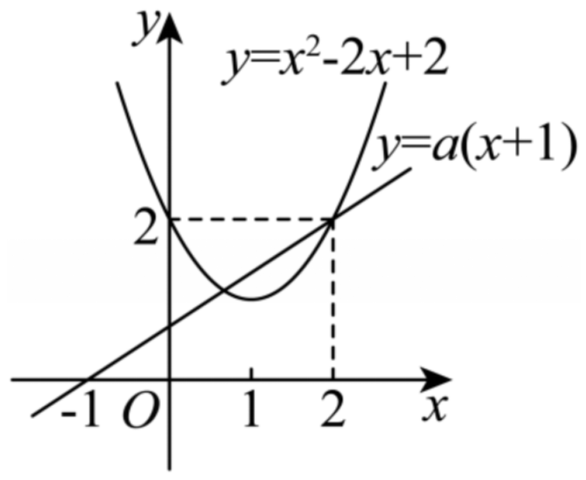
\includegraphics[width=0.30\textwidth]{figures/gao75_q12_graph.png}
\end{center}
% 原卷此处作“≥”，与题干严格不等号方向不一致，照录（见文件头“原卷笔误/存疑”①）
\step{由集合 $A$ 是“$2$ 集合”，故集合 $A$ 中只有一个元素，}
\step{得 $\begin{cases}2^2-2\times2+2\geqslant(2+1)a\\ 1^2-2\times1+2<(1+1)a\end{cases}$，解得 $\dfrac12<a\leqslant\dfrac23$，}
\step{故正实数 $a$ 的取值范围是 $\dfrac12<a\leqslant\dfrac23$.}
\solend
\fi

\end{enumerate}

\bigsec{二、选择题}

\begin{enumerate}
\setcounter{enumi}{12}

\item 已知全集 $U=\R$，集合 $A=\{x\mid x^2<4\}$，$B=\{y\mid y=x^2\}$，则图中阴影部分所表示的集合为\mbox{（\quad）}

\begin{center}
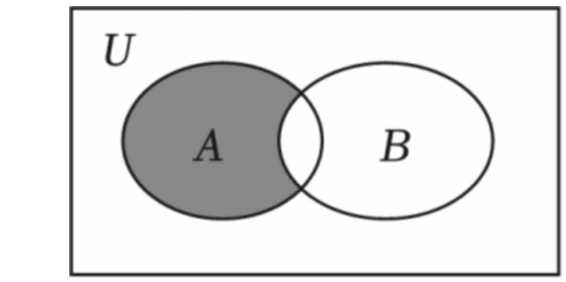
\includegraphics[width=0.26\textwidth]{figures/gao75_q13_venn.png}
\end{center}

\keepwithprev
A. $\{-2,-1,0\}$\qquad B. $(-\infty,4)$\qquad C. $(-2,0)$\qquad D. $(-2,0]$

\ifanswer
\solbegin
\step{集合 $A=\{x\mid x^2<4\}=(-2,2)$，$B=\{y\mid y=x^2\}=[0,+\infty)$，}
\step{图中阴影部分所表示的集合是 $A\cap\overline{B}=(-2,0)$. 故选 $C$.}
\solend
\fi

\item 已知 $x\in\R$，则“$\dfrac1x>1$”是“$x<1$”的\mbox{（\quad）}

\keepwithprev
A. 充分非必要条件\qquad B. 必要非充分条件\qquad C. 充要条件\qquad D. 既非充分又非必要条件

\ifanswer
\solbegin
\step{“$\dfrac1x>1$”$\Leftrightarrow0<x<1$，所以“$\dfrac1x>1$”是“$x<1$”的充分不必要条件. 故选 $A$.}
\solend
\fi

\item 已知集合 $M=\{x\mid x=m+\dfrac16,\,m\in\Z\}$，$N=\{x\mid x=\dfrac n2-\dfrac13,\,n\in\Z\}$，\\
$P=\{x\mid x=\dfrac p2+\dfrac16,\,p\in\Z\}$，则 $M$、$N$、$P$ 的关系为\mbox{（\quad）}

\keepwithprev
A. $M=N\subseteq P$\qquad B. $M\subseteq N=P$\qquad C. $M\subseteq N\subseteq P$\qquad D. $N\subseteq P\subseteq M$

\ifanswer
\solbegin
\step{集合 $N=\{x\mid x=\dfrac n2-\dfrac13,\,n\in\Z\}$，则 $x=\dfrac n2-\dfrac13=\dfrac{3n-2}6$，$n\in\Z$.}
\step{$P=\{x\mid x=\dfrac p2+\dfrac16,\,p\in\Z\}$，则 $x=\dfrac p2+\dfrac16=\dfrac{3p+1}6$，$p\in\Z$.}
\step{$M=\{x\mid x=m+\dfrac16,\,m\in\Z\}$，则 $x=m+\dfrac16=\dfrac{6m+1}6$，$m\in\Z$.}
\step{$M$、$N$、$P$ 三者分母相同，所以只需要比较他们的分子.}
\step{$M$：$6$ 的倍数$+1$，$N=P$：$3$ 的倍数$+1$，所以 $M\subseteq N=P$. 故选 $B$.}
\solend
\fi

\item 设集合 $P_1=\{x\mid x^2+ax+1>0\}$，$P_2=\{x\mid x^2+ax+2>0\}$，$Q_1=\{x\mid x^2+x+b>0\}$，$Q_2=\{x\mid x^2+2x+b>0\}$ 其中 $a,b\in\R$，给出下列两个命题：命题 $q_1$：对任意的 $a$，$P_1$ 是 $P_2$ 的子集；命题 $q_2$：对任意的 $b$，$Q_1$ 不是 $Q_2$ 的子集. 下列说法正确的是\mbox{（\quad）}

\keepwithprev
A. 命题 $q_1$ 是真命题，命题 $q_2$ 是假命题\qquad B. 命题 $q_1$ 是假命题，命题 $q_2$ 是真命题

C. 命题 $q_1$、$q_2$ 都是真命题\qquad D. 命题 $q_1$、$q_2$ 都是假命题

\ifanswer
\solbegin
\step{对于集合 $P_1=\{x\mid x^2+ax+1>0\}$，$P_2=\{x\mid x^2+ax+2>0\}$，}
\step{当 $m\in P_1$，即 $m^2+am+1>0$，得 $m^2+am+2>0$，}
\step{即有 $m\in P_2$，得对任意 $a$，$P_1$ 是 $P_2$ 的子集，命题 $q_1$ 为真命题；}
\step{当 $b=5$ 时，$Q_1=\{x\mid x^2+x+5>0\}=\R$，$Q_2=\{x\mid x^2+2x+5>0\}=\R$，}
\step{得 $Q_1$ 是 $Q_2$ 的子集；}
\step{存在 $b$，使得 $Q_1$ 是 $Q_2$ 的子集，故命题 $q_2$ 是假命题.}
\step{故选 $A$.}
\solend
\fi

\end{enumerate}

\bigsec{三、解答题}

\begin{enumerate}
\setcounter{enumi}{16}

\item 设集合 $A=\{x\mid x^2-2x=0\}$，$B=\{x\mid x^2+2(a+1)x+a^2-1=0\}$.

（1）写出集合 $A$ 的所有子集；

（2）若 $A\cap B=B$，求实数 $a$ 的取值范围.

\ifanswer
\solbegin
\stepm{(1)}{由 $x^2-2x=0$，得 $x=2$ 或 $x=0$，所以 $A=\{0,2\}$，}
\step{故集合 $A$ 的所有子集为 $\varnothing$、$\{0\}$、$\{2\}$、$\{0,2\}$.}
\stepm{(2)}{因为 $A\cap B=B$，所以 $B\subseteq A$，}
\step{方程 $x^2+2(a+1)x+a^2-1=0$，$\Delta=4(a+1)^2-4(a^2-1)=8a+8$，}
\step{若 $\Delta<0$，即 $a<-1$，方程 $x^2+2(a+1)x+a^2-1=0$ 无解，}
\step{此时 $B=\varnothing$，满足题意；}
\step{若 $\Delta=0$，即 $a=-1$，由 $x^2+2(a+1)x+a^2-1=0$，即 $x^2=0$，}
\step{解得 $x=0$，此时 $B=\{0\}$，满足题意；}
\step{若 $\Delta>0$，即 $a>-1$，要使 $B\subseteq A$，}
\step{则方程 $x^2+2(a+1)x+a^2-1=0$ 的解集为 $\{0,2\}$，}
\step{则 $\begin{cases}2+0=-2(a+1)\\ 2\times0=a^2-1\end{cases}$，$a$ 不存在.}
\step{综上所述，$a\leqslant-1$，即实数 $a$ 的取值范围为 $\{a\mid a\leqslant-1\}$.}
\solend
\fi

\ansspace

\item 已知全集 $U=\R$，集合 $A=\left\{x\,\middle|\,\dfrac{x-1}{x-3}<0\right\}$，$B=\{x\mid|x-a|<2\}$.

（1）当 $a=1$ 时，试用区间表示集合 $A$、$B$；

（2）若 $A\cup B=B$，求实数 $a$ 的取值范围.

\ifanswer
\solbegin
\stepm{(1)}{不等式 $\dfrac{x-1}{x-3}<0$ 可化为 $(x-1)(x-3)<0$，解得 $1<x<3$，即 $A=(1,3)$，}
\step{当 $a=1$ 时，$|x-1|<2$，则 $-2<x-1<2$，解得 $-1<x<3$，}
\step{即 $B=(-1,3)$；}
\stepm{(2)}{由不等式 $|x-a|<2$ 得 $-2<x-a<2$，解得 $-2+a<x<2+a$，}
\step{即 $B=\{x\mid-2+a<x<2+a\}$，}
\step{因为 $A\cup B=B$，所以 $A\subseteq B$，则 $\begin{cases}-2+a\leqslant1\\ 2+a\geqslant3\end{cases}$，解得 $1\leqslant a\leqslant3$，}
\step{即实数 $a$ 的取值范围为 $[1,3]$.}
\solend
\fi

\ansspace

\item 法国数学家弗朗索瓦·韦达 1615 年在著作《论方程的识别与订正》中建立了方程根与系数的关系. 发现一元二次方程 $ax^2+bx+c=0$，$a\neq0$ 的根与系数有如下的关系：

$x_1+x_2=-\dfrac ba$，$x_1x_2=\dfrac ca$，此即为韦达定理. 韦达定理的逆定理仍成立：如果两个数 $x_1$，$x_2$ 满足 $x_1+x_2=-\dfrac ba$，$x_1x_2=\dfrac ca$，则这两个数 $x_1$、$x_2$ 是方程 $ax^2+bx+c=0$，$a\neq0$ 的两个根. 例如：$m+n=-3$，$mn=2$，则 $m$、$n$ 是方程 $x^2+3x+2=0$ 的两个根. 请根据上述材料解决以下问题.

（1）已知 $m$、$n$ 是两个不相等的实数，满足 $m^2-6m-5=0$，$n^2-6n-5=0$，求 $\dfrac1m+\dfrac1n$ 的值；

（2）已知实数 $x$、$y$ 满足 $x+y+xy=17$，$x^2y+xy^2=72$，求 $x^2+y^2$ 的值.

\ifanswer
\solbegin
\stepm{(1)}{由题意，不相等的实数 $m$、$n$ 满足 $m^2-6m-5=0$、$n^2-6n-5=0$，}
\step{因此 $m$、$n$ 是一元二次方程 $x^2-6x-5=0$ 的两个不等实根.}
\step{由韦达定理得 $m+n=6$，$mn=-5$，因此 $\dfrac1m+\dfrac1n=\dfrac{m+n}{mn}=\dfrac6{-5}=-\dfrac65$.}
\stepm{(2)}{令 $s=x+y$，$t=xy$，}
\step{因为 $x+y+xy=17$，$x^2y+xy^2=72$，}
\step{即 $x+y+xy=17$，$xy(x+y)=72$，将已知条件变形得 $\begin{cases}s+t=17\\ st=72\end{cases}$.}
\step{由韦达定理逆定理，$s$、$t$ 是一元二次方程 $z^2-17z+72=0$ 的两个实根，}
\step{解方程得 $z_1=8$，$z_2=9$，即有两组解 $\begin{cases}s=8\\ t=9\end{cases}$ 和 $\begin{cases}s=9\\ t=8\end{cases}$.}
\step{当 $\begin{cases}s=8\\ t=9\end{cases}$ 时，$x$、$y$ 是方程 $w^2-8w+9=0$ 的根，}
\step{判别式 $\Delta=8^2-4\times1\times9=64-36=28>0$，符合题意，}
\step{此时 $x^2+y^2=(x+y)^2-2xy=s^2-2t=8^2-2\times9=64-18=46$；}
\step{当 $\begin{cases}s=9\\ t=8\end{cases}$ 时，$x$、$y$ 是方程 $w^2-9w+8=0$ 的根，}
\step{判别式 $\Delta=9^2-4\times1\times8=81-32=49>0$，符合题意，}
\step{此时 $x^2+y^2=(x+y)^2-2xy=s^2-2t=9^2-2\times8=81-16=65$.}
\step{综上，$x^2+y^2$ 的值为 $46$ 或 $65$.}
\solend
\fi

\ansspace

\item 已知关于 $x$ 的不等式 $ax^2-(a+1)x+b<0$.

（1）若不等式的解集是 $\{x\mid1<x<5\}$，求 $a+b$ 的值；

（2）若 $b=-\dfrac12$ 且不等式的解集为 $\R$，求 $a$ 取值范围；

（3）若 $b=1$，讨论此不等式的解集.

\ifanswer
\solbegin
\stepm{(1)}{由题意得 $1$ 和 $5$ 是方程 $ax^2-(a+1)x+b=0$ 的两个根且 $a>0$，}
\step{所以 $1+5=\dfrac{a+1}a$，$1\times5=\dfrac ba$，解得 $a=\dfrac15$，$b=1$，所以 $a+b=\dfrac65$.}
\stepm{(2)}{若 $b=-\dfrac12$，则不等式为 $ax^2-(a+1)x-\dfrac12<0$，}
\step{当 $a\neq0$，则有 $\begin{cases}a<0\\ \Delta=(a+1)^2+2a<0\end{cases}$，解得 $-2-\sqrt3<a<-2+\sqrt3$；}
\step{当 $a=0$，不等式即为 $-x-\dfrac12<0$，则 $x>-\dfrac12$，不合题意；}
\step{所以 $a$ 的取值范围是 $(-2-\sqrt3,-2+\sqrt3)$.}
\stepm{(3)}{若 $b=1$，则不等式为 $ax^2-(a+1)x+1<0$，即 $(ax-1)(x-1)<0$.}
\step{当 $a\neq0$ 时，由 $ax^2-(a+1)x+1<0$ 得 $(ax-1)(x-1)<0$.}
\step{方程 $(ax-1)(x-1)=0$ 的根为 $x=\dfrac1a$ 或 $x=1$，}
\step{当 $0<a<1$ 时，$\dfrac1a>1$，则不等式的解集为 $\left(1,\dfrac1a\right)$；}
\step{当 $a<0$ 时，$\dfrac1a<1$，则不等式的解集为 $\left(-\infty,\dfrac1a\right)\cup(1,+\infty)$；}
\step{当 $a=1$ 时，不等式即为 $(x-1)^2<0$，则不等式的解集为 $\varnothing$；}
\step{当 $a>1$ 时，$\dfrac1a<1$，则不等式的解集为 $\left(\dfrac1a,1\right)$；}
\step{当 $a=0$ 时，不等式为 $-x+1<0$，则不等式的解集为 $(1,+\infty)$；}
\step{综上所述，当 $a<0$ 时，不等式的解集为 $\left(-\infty,\dfrac1a\right)\cup(1,+\infty)$；}
\step{当 $a=0$ 时，不等式的解集为 $(1,+\infty)$；}
\step{当 $0<a<1$ 时，不等式的解集为 $\left(1,\dfrac1a\right)$；}
\step{当 $a=1$ 时，不等式的解集为 $\varnothing$；}
\step{当 $a>1$ 时，不等式的解集为 $\left(\dfrac1a,1\right)$.}
\solend
\fi

\ansspace

\item 已知关于 $x$ 的不等式① $x^2+2cx+c>0$，② $x^2+cx+c^2-1>0$，其中 $c$ 是实数.

（1）若 $1$ 是不等式②的一个解，求实数 $c$ 的取值范围；

（2）证明：不等式①、②中至多有一个恒成立；

（3）当 $c=0$ 时，“$x$ 满足 $|mx^2-4x+3|>5$”的一个必要非充分条件是“$x$ 满足 $x^2+cx+c^2-1>0$，求实数 $m$ 的取值范围.

\ifanswer
\solbegin
\stepm{(1)}{因为 $1$ 是不等式②的一个解，所以 $1+c+c^2-1>0$，}
\step{即 $c(c+1)>0$，解得 $c>0$ 或 $c<-1$，}
\step{所以实数 $c$ 的取值范围为 $(-\infty,-1)\cup(0,+\infty)$.}
\stepm{(2)}{假设不等式①、②都恒成立，}
\step{不等式① $x^2+2cx+c>0$ 恒成立，所以 $4c^2-4c<0$，所以 $0<c<1$；}
\step{② $x^2+cx+c^2-1>0$ 恒成立，所以 $c^2-4(c^2-1)<0$，$c^2>\dfrac43$，}
\step{解得 $c>\dfrac{2\sqrt3}3$ 或 $c<-\dfrac{2\sqrt3}3$；}
\step{所以当不等式①、②都恒成立时，}
\step{不等式组 $\begin{cases}0<c<1\\ c\in\left(-\infty,-\dfrac{2\sqrt3}3\right)\cup\left(\dfrac{2\sqrt3}3,+\infty\right)\end{cases}$ 无解，}
\step{所以假设不成立，}
\step{所以不等式①、②中至多有一个恒成立.}
\stepm{(3)}{当 $c=0$ 时，由 $x^2+cx+c^2-1>0$ 得 $x^2-1>0$，}
\step{解集为 $(-\infty,-1)\cup(1,+\infty)$.}
\step{记集合 $A=\{x\mid|mx^2-4x+3|>5\}$，集合 $B=\{x\mid x<-1\text{ 或 }x>1\}$.}
\step{由“$x$ 满足 $|mx^2-4x+3|>5$”的一个必要非充分条件是}
\step{“$x$ 满足 $x^2+cx+c^2-1>0$”得 $A$ 是 $B$ 的真子集.}
\step{所以 $\overline{B}$ 是 $A$ 的真子集，即对任意 $x\in[-1,1]$，$|mx^2-4x+3|\leqslant5$ 恒成立.}
\step{当 $x=0$ 时，不等式 $-5\leqslant mx^2-4x+3\leqslant5$ 恒成立；}
\step{当 $x\in[-1,0)\cup(0,1]$ 时，}
\step{则 $mx^2-4x+3\geqslant-5$ 与 $mx^2-4x+3\leqslant5$ 同时成立.}
\step{①由 $mx^2-4x+3\geqslant-5$，得 $m\geqslant\dfrac{4x-8}{x^2}$，求值域得 $\dfrac{4x-8}{x^2}$ 的最大值 $=-4$，}
\step{所以 $m\geqslant-4$.}
\step{②由 $mx^2-4x+3\leqslant5$，得 $m\leqslant\dfrac{4x+2}{x^2}$，求值域得 $\dfrac{4x+2}{x^2}$ 的最小值 $=-2$，}
\step{所以 $m\leqslant-2$.}
\step{综上所述，实数 $m$ 的取值范围为 $[-4,-2]$.}
\solend
\fi

\ansspace*[7]

\end{enumerate}

\end{document}
"
%
% 原始材料：微信公众号“魔都数学加油站”文章，连载“27学年高一75”；
% 原文标题“27学年高一75——2026-2027年上海市市二中学高一上10月月考”；
% 原文链接：https://mp.weixin.qq.com/s/dhxtwWEZgKLxeKdkbWqOhw。
% 页面标注发布时间 2026-10-22 21:45（上海）。
% 正文为 11 张 PNG 页（`原图/高一75_市二中学_10月月考/01..11.png`）：
% 第 2、4、5、6、9 页为 4762×6735，其余 6 页为 2560×3620，均按页序读取。
% 11 页全为试卷正文页（卷首标题在第 1 页页顶，卷末第 21 题 (3) 解析止于第 11 页），
% 无封面页、目录页、二维码或宣传页。粉色斜排“魔都数学加油站”为卷面水印，未录入。
%
% 卷首标题：照卷面印作“2026-2027 年市二中学高一上 10 月月考”（黑体加粗一行）。
% 原卷年份区间用半角连字符，本稿按全稿惯例排 en dash；原卷无副标题。
%
% 篇幅与题号：原卷自第 3 题起编号（第 1、2 题不在本卷内）。填空题 3—12（10 题）、
% 选择题 13—16（4 题）、解答题 17—21（5 题），共 19 题。本稿沿用原节与原题号，
% 只改排为全稿统一的大节样式。
%
% 讲评版：原卷第 4 题只印【答案】（“$[-1,2]$”），本稿只给 \ans{}；其余 18 题均印
% 【解析】，用 \solbegin…\solend。四道选择题的作答括号原卷即留空，答案写在解析末句
% “故选 C／A／B／A”，照录在解析内，不另提 \ans{}。
%
% 副标题：原卷未印副标题。本稿按“知识模块”口径标作“集合与常用逻辑用语、不等式”：
% 19 题中集合与常用逻辑用语 9 题（第 3、4、5、8、10、12、13、15、17、18 题中的集合题），
% 不等式 10 题（第 6、7、9、11、19、20、21 题及第 12、20 题的不等式部分），两类均确有
% 分量，故并标。口径同 高一63、高一68—74。
%
% 与原卷的排版差异：
%   ① 原卷每题下直接印【答案】/【解析】，本稿按全稿惯例将答案与解析置于答案版；
%   ② 原卷未印副标题，本稿按“知识模块”口径补出；
%   ③ 原卷填空横线约四个字宽，本稿按全稿惯例统一排 \blankline[4.4em]；
%   ④ 原卷数集记号排粗体 $\mathbf{R}$（第 5、6、7、9、10、14、18、20、21 题），本稿
%      按全稿惯例改用 $\R$（同 高一68—74）；第 11 题的“解集为 $\R$”同此；
%   ⑤ 原卷句末标点多为西文句点，均逐处照录；
%   ⑥ 第 17—21 题的子问原卷印作“（1）…（2）…”，本稿按 高一69—74 成例用行内
%      “（1）（2）（3）”段，解析中的子问标号用 \stepm{(1)}{…}；
%   ⑦ 每道解答题原卷未留作答空白，本稿按全稿惯例加 \ansspace（末题用 \ansspace*）；
%   ⑧ 选择题的作答括号原卷排半角“(    )”，本稿按全稿惯例排 \mbox{（\quad）}；
%      选项行排照原卷——第 13、14 题一行四条，第 15、16 题一行四条；
%   ⑨ 第 9、12、15、17—21 题解析中的不等式组／方程组，原卷均排作“{”连接的多行式，
%      本稿按全稿惯例排 cases；
%   ⑩ 第 12 题解析有一幅“抛物线 + 直线”图：原卷印在解析第 3 行右侧、题干无“如图”二字
%      （解析里写“两函数图象如图：”）。本稿按原卷截图裁取（`figures/gao75_q12_graph.png`，
%      由第 3 页原图裁出、去除粉色水印后转灰度，未放大），放在答案版解析第 3 条之后；
%   ⑪ 第 13 题题干中间有一幅韦恩图（全集矩形内含 A、B 两圆，A 涂灰）：原卷印在题干
%      右侧、题干句子被图隔开。本稿按原卷截图裁取（`figures/gao75_q13_venn.png`，由第 3
%      页原图裁出、去除粉色水印后转灰度，并抹去左侧侵入的“分”字），放在题干之后、
%      选项之前，仅答案版出。
%
% 原卷笔误/存疑（均照录未改，正文对应处另有 % 注）：
%   ① 第 12 题解析列不等式组时写 $2^2-2\times2+2\geqslant(2+1)a$，与
%      $x^2-2x+2<a(x+1)$ 的严格不等号方向不一致；原卷如此，照录未改。
%   ② 第 14 题选项 A—D 的“充分非必要”“必要非充分”“既非充分又非必要”与原卷
%      其它题的“充分不必要”写法不同，照录未统一。
%   ④ 第 21 题 (3) 题干的“$x$ 满足 $|mx^2-4x+3|>5$”的一个必要非充分条件是
%      “$x$ 满足 $x^2+cx+c^2-1>0$，原卷只有左引号、无右引号（且逗号在引号内），
%      本稿照录未补。
%   ③ 第 20 题 (2) 的解集写成 $(-2-\sqrt3,-2+\sqrt3)$，其中 $a<0$ 与 $\Delta<0$ 联立后
%      左端点应为 $-2-\sqrt3$、右端点为 $-2+\sqrt3$；原卷如此，照录未改。
%
% 行数核对：逐题数 \step/\stepm 条数与原卷【解析】印刷行数，18 题逐一相符，
% 合计 132 条 / 132 行（Q3：6；Q5：1；Q6：2；Q7：1；Q8：2；Q9：3；Q10：10；
% Q11：8；Q12：6；Q13：2；Q14：1；Q15：5；Q16：7；Q17：12；Q18：7；Q19：15；
% Q20：19；Q21：25）。另第 4 题只印【答案】，提 \ans{}，不计入 \step 账。
%
% 插图：第 12 题解析的抛物线图、第 13 题题干的韦恩图，见上⑩⑪；其余题干无配图。
%
\documentclass[a4paper,11pt]{article}
\usepackage{common}

\begin{document}

\examtitlest[3]{2026--2027 年市二中学高一上 10 月月考}{集合与常用逻辑用语、不等式}

\bigsec{一、填空题}

\begin{enumerate}
\setcounter{enumi}{2}

\item 已知集合 $A=\{a,a^2\}$，且 $1\in A$，则 $a=$\blankline[4.4em].

\ifanswer
\solbegin
\step{因为 $1\in A=\{a,a^2\}$，所以 $a=1$ 或 $a^2=1$.}
\step{又集合 $A=\{a,a^2\}$ 是用列举法写出两个元素的，其元素必须互异，故 $a\neq a^2$，}
\step{即 $a\neq0$ 且 $a\neq1$，所以 $a=1$ 应舍去；}
\step{由 $a^2=1$ 得 $a=1$（舍去）或 $a=-1$.}
\step{当 $a=-1$ 时，$A=\{-1,1\}$，满足 $1\in A$ 且两个元素互异.}
\step{故 $a=-1$.}
\solend
\fi

\item 已知集合 $A=[-1,1]$，$B=[0,2]$，则 $A\cup B=$\blankline[4.4em].

\ifanswer
\ans{$[-1,2]$}
\fi

\item 已知全集 $U=\R$，集合 $A=\{x\mid x\neq1\}$，则 $\overline{A}=$\blankline[4.4em].

\ifanswer
\solbegin
\step{因为全集 $U=\R$，集合 $A=\{x\mid x\neq1\}$，所以 $\overline{A}=\{x\mid x=1\}$.}
\solend
\fi

\item 设 $x\in\R$，不等式 $x^2-4x<0$ 的解集用区间表示是\blankline[4.4em].

\ifanswer
\solbegin
\step{因为 $x^2-4x<0$，即 $x(x-4)<0$，所以 $0<x<4$，}
\step{所以 $x(x-4)<0$ 的解集为 $(0,4)$.}
\solend
\fi

\item 已知 $m\in\R$，若关于 $x$ 的方程 $2mx^2+3x+m-1=m^2\cdot x^2+(m+1)x+1$ 解集为 $\R$，则 $m$ 的值为\blankline[4.4em].

\ifanswer
\solbegin
\step{由题意得 $2m=m^2$，$3=m+1$，$m-1=1$，所以 $m=2$.}
\solend
\fi

\item 设 $\alpha:x\leqslant m$，$\beta:|x-2|\leqslant1$，若 $\alpha$ 是 $\beta$ 的必要条件，则实数 $m$ 的取值范围是\blankline[4.4em].

\ifanswer
\solbegin
\step{由 $|x-2|\leqslant1$，得 $-1\leqslant x-2\leqslant1$，解得 $1\leqslant x\leqslant3$，}
\step{因为 $\alpha$ 是 $\beta$ 的必要条件，所以 $\{x\mid1\leqslant x\leqslant3\}\subseteq\{x\mid x\leqslant m\}$，得 $m\geqslant3$.}
\solend
\fi

\item 设 $a\in\R$，若关于 $x$ 的不等式 $\dfrac{a}{x-1}\leqslant1$ 的解集是 $(-\infty,1)\cup[2,+\infty)$，则 $a$ 的值为\blankline[4.4em].

\ifanswer
\solbegin
\step{不等式可变形为 $\dfrac{a+1-x}{x-1}\leqslant0$，等价于 $\begin{cases}(a+1-x)(x-1)\leqslant0\\ x-1\neq0\end{cases}$，}
\step{因为原不等式的解集是 $(-\infty,1)\cup[2,+\infty)$，}
\step{所以 $1$，$2$ 是方程 $(a+1-x)(x-1)=0$ 的两根，所以 $a+1=2$，解得 $a=1$.}
\solend
\fi

\item 下列命题：① “$x>1$ 或 $y>1$”的否定形式是“$x\leqslant1$ 或 $y\leqslant1$”，② 若 $A\cup B=B$，则 $A\subseteq B$，③ 方程 $ax+1=0$ 的解是 $x=-\frac1a$，④ “$ac=bc$”是“$a=b$”的必要非充分条件，⑤ “任意 $x\in\R$，$f(x)=f(-x)$”的否定形式是“存在 $x_0\in\R$，使得 $f(x_0)\neq f(-x_0)$”其中真命题的序号是\blankline[4.4em]（填写序号）.

\ifanswer
\solbegin
\step{①假命题：“$x>1$ 或 $y>1$”的否定形式是“$x\leqslant1$ 且 $y\leqslant1$”；}
\step{②真命题：$A\cup B=B\Leftrightarrow A\subseteq B$；}
\step{③假命题：当 $a=0$ 时，方程无解，因此该命题忽略了 $a=0$ 的情况；}
\step{④真命题：先判断必要性：若 $a=b$，则有 $ac=bc$，所以必要性成立；}
\step{再判断充分性：若 $ac=bc$，即 $(a-b)c=0$，当 $c=0$ 时，$a$ 和 $b$ 可以不相等，}
\step{因此充分性不成立.}
\step{⑤真命题：全称命题的否定是存在量词命题，}
\step{“任意 $x\in\R$，$f(x)=f(-x)$”的否定形式是}
\step{“存在 $x_0\in\R$，使得 $f(x_0)\neq f(-x_0)$”，表述正确.}
\step{故正确的是②④⑤.}
\solend
\fi

\item 为了加强家校联系，蔡老师组建了一个由学生、家长和教师组成的微信群. 已知该群中男学生人数多于女学生人数，女学生人数多于家长人数，家长人数多于教师人数，教师人数的两倍多于男学生人数. 则该微信群人数的最小值为\blankline[4.4em].

\ifanswer
\solbegin
\step{设男学生、女学生、家长、教师的人数分别为 $M$、$F$、$P$、$T$，}
\step{它们都是正整数.}
\step{由题意得 $M>F>P>T$，且教师人数的两倍多于男学生人数，即 $2T>M$.}
\step{由 $M>F>P>T$ 得 $M\geqslant T+3$；}
\step{又 $2T>M\geqslant T+3$，所以 $2T>T+3$，解得 $T>3$，故教师人数最少为 $T=4$.}
\step{当 $T=4$ 时，为使总人数最少，取 $P=5$、$F=6$、$M=7$，}
\step{此时 $7>6>5>4$ 且 $2\times4=8>7$，满足题意.}
\step{于是微信群人数为 $4+5+6+7=22$，所以该微信群人数的最小值为 $22$.}
\solend
\fi

\item 若集合 $M$ 有 $k$ 个子集，则称集合 $M$ 为“$k$ 集合”，\\
已知集合 $A=\{x\mid x^2-(a+2)x+2-a<0,\,x\in\Z\}$ 是“$2$ 集合”，则正实数 $a$ 的取值范围是\blankline[4.4em].

\ifanswer
\solbegin
\step{由 $x^2-(a+2)x+2-a<0$，得 $x^2-2x+2<a(x+1)$，}
\step{设二次函数 $y=x^2-2x+2$ 与一次函数 $y=a(x+1)$，}
\needvspace{13\baselineskip}
\step{由 $a>0$，$y=a(x+1)$ 过定点 $(-1,0)$，两函数图象如图：}
\begin{center}
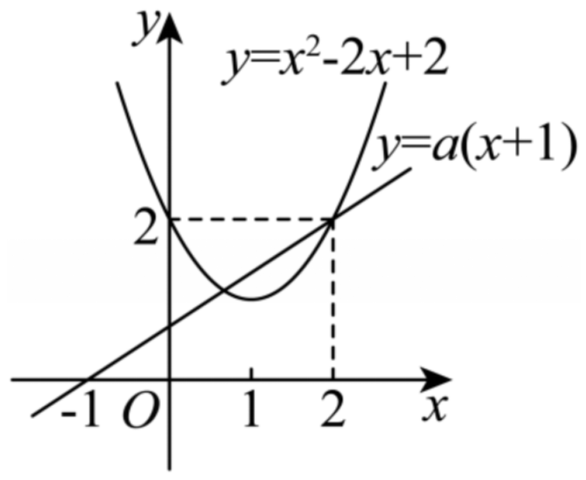
\includegraphics[width=0.30\textwidth]{figures/gao75_q12_graph.png}
\end{center}
% 原卷此处作“≥”，与题干严格不等号方向不一致，照录（见文件头“原卷笔误/存疑”①）
\step{由集合 $A$ 是“$2$ 集合”，故集合 $A$ 中只有一个元素，}
\step{得 $\begin{cases}2^2-2\times2+2\geqslant(2+1)a\\ 1^2-2\times1+2<(1+1)a\end{cases}$，解得 $\dfrac12<a\leqslant\dfrac23$，}
\step{故正实数 $a$ 的取值范围是 $\dfrac12<a\leqslant\dfrac23$.}
\solend
\fi

\end{enumerate}

\bigsec{二、选择题}

\begin{enumerate}
\setcounter{enumi}{12}

\item 已知全集 $U=\R$，集合 $A=\{x\mid x^2<4\}$，$B=\{y\mid y=x^2\}$，则图中阴影部分所表示的集合为\mbox{（\quad）}

\begin{center}
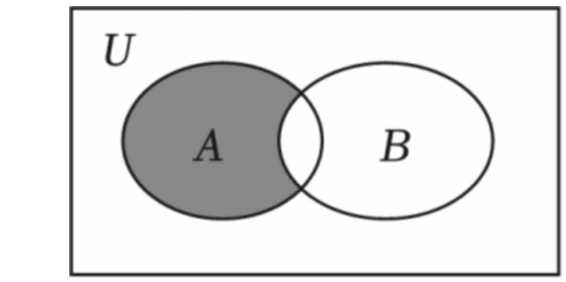
\includegraphics[width=0.26\textwidth]{figures/gao75_q13_venn.png}
\end{center}

\keepwithprev
A. $\{-2,-1,0\}$\qquad B. $(-\infty,4)$\qquad C. $(-2,0)$\qquad D. $(-2,0]$

\ifanswer
\solbegin
\step{集合 $A=\{x\mid x^2<4\}=(-2,2)$，$B=\{y\mid y=x^2\}=[0,+\infty)$，}
\step{图中阴影部分所表示的集合是 $A\cap\overline{B}=(-2,0)$. 故选 $C$.}
\solend
\fi

\item 已知 $x\in\R$，则“$\dfrac1x>1$”是“$x<1$”的\mbox{（\quad）}

\keepwithprev
A. 充分非必要条件\qquad B. 必要非充分条件\qquad C. 充要条件\qquad D. 既非充分又非必要条件

\ifanswer
\solbegin
\step{“$\dfrac1x>1$”$\Leftrightarrow0<x<1$，所以“$\dfrac1x>1$”是“$x<1$”的充分不必要条件. 故选 $A$.}
\solend
\fi

\item 已知集合 $M=\{x\mid x=m+\dfrac16,\,m\in\Z\}$，$N=\{x\mid x=\dfrac n2-\dfrac13,\,n\in\Z\}$，\\
$P=\{x\mid x=\dfrac p2+\dfrac16,\,p\in\Z\}$，则 $M$、$N$、$P$ 的关系为\mbox{（\quad）}

\keepwithprev
A. $M=N\subseteq P$\qquad B. $M\subseteq N=P$\qquad C. $M\subseteq N\subseteq P$\qquad D. $N\subseteq P\subseteq M$

\ifanswer
\solbegin
\step{集合 $N=\{x\mid x=\dfrac n2-\dfrac13,\,n\in\Z\}$，则 $x=\dfrac n2-\dfrac13=\dfrac{3n-2}6$，$n\in\Z$.}
\step{$P=\{x\mid x=\dfrac p2+\dfrac16,\,p\in\Z\}$，则 $x=\dfrac p2+\dfrac16=\dfrac{3p+1}6$，$p\in\Z$.}
\step{$M=\{x\mid x=m+\dfrac16,\,m\in\Z\}$，则 $x=m+\dfrac16=\dfrac{6m+1}6$，$m\in\Z$.}
\step{$M$、$N$、$P$ 三者分母相同，所以只需要比较他们的分子.}
\step{$M$：$6$ 的倍数$+1$，$N=P$：$3$ 的倍数$+1$，所以 $M\subseteq N=P$. 故选 $B$.}
\solend
\fi

\item 设集合 $P_1=\{x\mid x^2+ax+1>0\}$，$P_2=\{x\mid x^2+ax+2>0\}$，$Q_1=\{x\mid x^2+x+b>0\}$，$Q_2=\{x\mid x^2+2x+b>0\}$ 其中 $a,b\in\R$，给出下列两个命题：命题 $q_1$：对任意的 $a$，$P_1$ 是 $P_2$ 的子集；命题 $q_2$：对任意的 $b$，$Q_1$ 不是 $Q_2$ 的子集. 下列说法正确的是\mbox{（\quad）}

\keepwithprev
A. 命题 $q_1$ 是真命题，命题 $q_2$ 是假命题\qquad B. 命题 $q_1$ 是假命题，命题 $q_2$ 是真命题

C. 命题 $q_1$、$q_2$ 都是真命题\qquad D. 命题 $q_1$、$q_2$ 都是假命题

\ifanswer
\solbegin
\step{对于集合 $P_1=\{x\mid x^2+ax+1>0\}$，$P_2=\{x\mid x^2+ax+2>0\}$，}
\step{当 $m\in P_1$，即 $m^2+am+1>0$，得 $m^2+am+2>0$，}
\step{即有 $m\in P_2$，得对任意 $a$，$P_1$ 是 $P_2$ 的子集，命题 $q_1$ 为真命题；}
\step{当 $b=5$ 时，$Q_1=\{x\mid x^2+x+5>0\}=\R$，$Q_2=\{x\mid x^2+2x+5>0\}=\R$，}
\step{得 $Q_1$ 是 $Q_2$ 的子集；}
\step{存在 $b$，使得 $Q_1$ 是 $Q_2$ 的子集，故命题 $q_2$ 是假命题.}
\step{故选 $A$.}
\solend
\fi

\end{enumerate}

\bigsec{三、解答题}

\begin{enumerate}
\setcounter{enumi}{16}

\item 设集合 $A=\{x\mid x^2-2x=0\}$，$B=\{x\mid x^2+2(a+1)x+a^2-1=0\}$.

（1）写出集合 $A$ 的所有子集；

（2）若 $A\cap B=B$，求实数 $a$ 的取值范围.

\ifanswer
\solbegin
\stepm{(1)}{由 $x^2-2x=0$，得 $x=2$ 或 $x=0$，所以 $A=\{0,2\}$，}
\step{故集合 $A$ 的所有子集为 $\varnothing$、$\{0\}$、$\{2\}$、$\{0,2\}$.}
\stepm{(2)}{因为 $A\cap B=B$，所以 $B\subseteq A$，}
\step{方程 $x^2+2(a+1)x+a^2-1=0$，$\Delta=4(a+1)^2-4(a^2-1)=8a+8$，}
\step{若 $\Delta<0$，即 $a<-1$，方程 $x^2+2(a+1)x+a^2-1=0$ 无解，}
\step{此时 $B=\varnothing$，满足题意；}
\step{若 $\Delta=0$，即 $a=-1$，由 $x^2+2(a+1)x+a^2-1=0$，即 $x^2=0$，}
\step{解得 $x=0$，此时 $B=\{0\}$，满足题意；}
\step{若 $\Delta>0$，即 $a>-1$，要使 $B\subseteq A$，}
\step{则方程 $x^2+2(a+1)x+a^2-1=0$ 的解集为 $\{0,2\}$，}
\step{则 $\begin{cases}2+0=-2(a+1)\\ 2\times0=a^2-1\end{cases}$，$a$ 不存在.}
\step{综上所述，$a\leqslant-1$，即实数 $a$ 的取值范围为 $\{a\mid a\leqslant-1\}$.}
\solend
\fi

\ansspace

\item 已知全集 $U=\R$，集合 $A=\left\{x\,\middle|\,\dfrac{x-1}{x-3}<0\right\}$，$B=\{x\mid|x-a|<2\}$.

（1）当 $a=1$ 时，试用区间表示集合 $A$、$B$；

（2）若 $A\cup B=B$，求实数 $a$ 的取值范围.

\ifanswer
\solbegin
\stepm{(1)}{不等式 $\dfrac{x-1}{x-3}<0$ 可化为 $(x-1)(x-3)<0$，解得 $1<x<3$，即 $A=(1,3)$，}
\step{当 $a=1$ 时，$|x-1|<2$，则 $-2<x-1<2$，解得 $-1<x<3$，}
\step{即 $B=(-1,3)$；}
\stepm{(2)}{由不等式 $|x-a|<2$ 得 $-2<x-a<2$，解得 $-2+a<x<2+a$，}
\step{即 $B=\{x\mid-2+a<x<2+a\}$，}
\step{因为 $A\cup B=B$，所以 $A\subseteq B$，则 $\begin{cases}-2+a\leqslant1\\ 2+a\geqslant3\end{cases}$，解得 $1\leqslant a\leqslant3$，}
\step{即实数 $a$ 的取值范围为 $[1,3]$.}
\solend
\fi

\ansspace

\item 法国数学家弗朗索瓦·韦达 1615 年在著作《论方程的识别与订正》中建立了方程根与系数的关系. 发现一元二次方程 $ax^2+bx+c=0$，$a\neq0$ 的根与系数有如下的关系：

$x_1+x_2=-\dfrac ba$，$x_1x_2=\dfrac ca$，此即为韦达定理. 韦达定理的逆定理仍成立：如果两个数 $x_1$，$x_2$ 满足 $x_1+x_2=-\dfrac ba$，$x_1x_2=\dfrac ca$，则这两个数 $x_1$、$x_2$ 是方程 $ax^2+bx+c=0$，$a\neq0$ 的两个根. 例如：$m+n=-3$，$mn=2$，则 $m$、$n$ 是方程 $x^2+3x+2=0$ 的两个根. 请根据上述材料解决以下问题.

（1）已知 $m$、$n$ 是两个不相等的实数，满足 $m^2-6m-5=0$，$n^2-6n-5=0$，求 $\dfrac1m+\dfrac1n$ 的值；

（2）已知实数 $x$、$y$ 满足 $x+y+xy=17$，$x^2y+xy^2=72$，求 $x^2+y^2$ 的值.

\ifanswer
\solbegin
\stepm{(1)}{由题意，不相等的实数 $m$、$n$ 满足 $m^2-6m-5=0$、$n^2-6n-5=0$，}
\step{因此 $m$、$n$ 是一元二次方程 $x^2-6x-5=0$ 的两个不等实根.}
\step{由韦达定理得 $m+n=6$，$mn=-5$，因此 $\dfrac1m+\dfrac1n=\dfrac{m+n}{mn}=\dfrac6{-5}=-\dfrac65$.}
\stepm{(2)}{令 $s=x+y$，$t=xy$，}
\step{因为 $x+y+xy=17$，$x^2y+xy^2=72$，}
\step{即 $x+y+xy=17$，$xy(x+y)=72$，将已知条件变形得 $\begin{cases}s+t=17\\ st=72\end{cases}$.}
\step{由韦达定理逆定理，$s$、$t$ 是一元二次方程 $z^2-17z+72=0$ 的两个实根，}
\step{解方程得 $z_1=8$，$z_2=9$，即有两组解 $\begin{cases}s=8\\ t=9\end{cases}$ 和 $\begin{cases}s=9\\ t=8\end{cases}$.}
\step{当 $\begin{cases}s=8\\ t=9\end{cases}$ 时，$x$、$y$ 是方程 $w^2-8w+9=0$ 的根，}
\step{判别式 $\Delta=8^2-4\times1\times9=64-36=28>0$，符合题意，}
\step{此时 $x^2+y^2=(x+y)^2-2xy=s^2-2t=8^2-2\times9=64-18=46$；}
\step{当 $\begin{cases}s=9\\ t=8\end{cases}$ 时，$x$、$y$ 是方程 $w^2-9w+8=0$ 的根，}
\step{判别式 $\Delta=9^2-4\times1\times8=81-32=49>0$，符合题意，}
\step{此时 $x^2+y^2=(x+y)^2-2xy=s^2-2t=9^2-2\times8=81-16=65$.}
\step{综上，$x^2+y^2$ 的值为 $46$ 或 $65$.}
\solend
\fi

\ansspace

\item 已知关于 $x$ 的不等式 $ax^2-(a+1)x+b<0$.

（1）若不等式的解集是 $\{x\mid1<x<5\}$，求 $a+b$ 的值；

（2）若 $b=-\dfrac12$ 且不等式的解集为 $\R$，求 $a$ 取值范围；

（3）若 $b=1$，讨论此不等式的解集.

\ifanswer
\solbegin
\stepm{(1)}{由题意得 $1$ 和 $5$ 是方程 $ax^2-(a+1)x+b=0$ 的两个根且 $a>0$，}
\step{所以 $1+5=\dfrac{a+1}a$，$1\times5=\dfrac ba$，解得 $a=\dfrac15$，$b=1$，所以 $a+b=\dfrac65$.}
\stepm{(2)}{若 $b=-\dfrac12$，则不等式为 $ax^2-(a+1)x-\dfrac12<0$，}
\step{当 $a\neq0$，则有 $\begin{cases}a<0\\ \Delta=(a+1)^2+2a<0\end{cases}$，解得 $-2-\sqrt3<a<-2+\sqrt3$；}
\step{当 $a=0$，不等式即为 $-x-\dfrac12<0$，则 $x>-\dfrac12$，不合题意；}
\step{所以 $a$ 的取值范围是 $(-2-\sqrt3,-2+\sqrt3)$.}
\stepm{(3)}{若 $b=1$，则不等式为 $ax^2-(a+1)x+1<0$，即 $(ax-1)(x-1)<0$.}
\step{当 $a\neq0$ 时，由 $ax^2-(a+1)x+1<0$ 得 $(ax-1)(x-1)<0$.}
\step{方程 $(ax-1)(x-1)=0$ 的根为 $x=\dfrac1a$ 或 $x=1$，}
\step{当 $0<a<1$ 时，$\dfrac1a>1$，则不等式的解集为 $\left(1,\dfrac1a\right)$；}
\step{当 $a<0$ 时，$\dfrac1a<1$，则不等式的解集为 $\left(-\infty,\dfrac1a\right)\cup(1,+\infty)$；}
\step{当 $a=1$ 时，不等式即为 $(x-1)^2<0$，则不等式的解集为 $\varnothing$；}
\step{当 $a>1$ 时，$\dfrac1a<1$，则不等式的解集为 $\left(\dfrac1a,1\right)$；}
\step{当 $a=0$ 时，不等式为 $-x+1<0$，则不等式的解集为 $(1,+\infty)$；}
\step{综上所述，当 $a<0$ 时，不等式的解集为 $\left(-\infty,\dfrac1a\right)\cup(1,+\infty)$；}
\step{当 $a=0$ 时，不等式的解集为 $(1,+\infty)$；}
\step{当 $0<a<1$ 时，不等式的解集为 $\left(1,\dfrac1a\right)$；}
\step{当 $a=1$ 时，不等式的解集为 $\varnothing$；}
\step{当 $a>1$ 时，不等式的解集为 $\left(\dfrac1a,1\right)$.}
\solend
\fi

\ansspace

\item 已知关于 $x$ 的不等式① $x^2+2cx+c>0$，② $x^2+cx+c^2-1>0$，其中 $c$ 是实数.

（1）若 $1$ 是不等式②的一个解，求实数 $c$ 的取值范围；

（2）证明：不等式①、②中至多有一个恒成立；

（3）当 $c=0$ 时，“$x$ 满足 $|mx^2-4x+3|>5$”的一个必要非充分条件是“$x$ 满足 $x^2+cx+c^2-1>0$，求实数 $m$ 的取值范围.

\ifanswer
\solbegin
\stepm{(1)}{因为 $1$ 是不等式②的一个解，所以 $1+c+c^2-1>0$，}
\step{即 $c(c+1)>0$，解得 $c>0$ 或 $c<-1$，}
\step{所以实数 $c$ 的取值范围为 $(-\infty,-1)\cup(0,+\infty)$.}
\stepm{(2)}{假设不等式①、②都恒成立，}
\step{不等式① $x^2+2cx+c>0$ 恒成立，所以 $4c^2-4c<0$，所以 $0<c<1$；}
\step{② $x^2+cx+c^2-1>0$ 恒成立，所以 $c^2-4(c^2-1)<0$，$c^2>\dfrac43$，}
\step{解得 $c>\dfrac{2\sqrt3}3$ 或 $c<-\dfrac{2\sqrt3}3$；}
\step{所以当不等式①、②都恒成立时，}
\step{不等式组 $\begin{cases}0<c<1\\ c\in\left(-\infty,-\dfrac{2\sqrt3}3\right)\cup\left(\dfrac{2\sqrt3}3,+\infty\right)\end{cases}$ 无解，}
\step{所以假设不成立，}
\step{所以不等式①、②中至多有一个恒成立.}
\stepm{(3)}{当 $c=0$ 时，由 $x^2+cx+c^2-1>0$ 得 $x^2-1>0$，}
\step{解集为 $(-\infty,-1)\cup(1,+\infty)$.}
\step{记集合 $A=\{x\mid|mx^2-4x+3|>5\}$，集合 $B=\{x\mid x<-1\text{ 或 }x>1\}$.}
\step{由“$x$ 满足 $|mx^2-4x+3|>5$”的一个必要非充分条件是}
\step{“$x$ 满足 $x^2+cx+c^2-1>0$”得 $A$ 是 $B$ 的真子集.}
\step{所以 $\overline{B}$ 是 $A$ 的真子集，即对任意 $x\in[-1,1]$，$|mx^2-4x+3|\leqslant5$ 恒成立.}
\step{当 $x=0$ 时，不等式 $-5\leqslant mx^2-4x+3\leqslant5$ 恒成立；}
\step{当 $x\in[-1,0)\cup(0,1]$ 时，}
\step{则 $mx^2-4x+3\geqslant-5$ 与 $mx^2-4x+3\leqslant5$ 同时成立.}
\step{①由 $mx^2-4x+3\geqslant-5$，得 $m\geqslant\dfrac{4x-8}{x^2}$，求值域得 $\dfrac{4x-8}{x^2}$ 的最大值 $=-4$，}
\step{所以 $m\geqslant-4$.}
\step{②由 $mx^2-4x+3\leqslant5$，得 $m\leqslant\dfrac{4x+2}{x^2}$，求值域得 $\dfrac{4x+2}{x^2}$ 的最小值 $=-2$，}
\step{所以 $m\leqslant-2$.}
\step{综上所述，实数 $m$ 的取值范围为 $[-4,-2]$.}
\solend
\fi

\ansspace*[7]

\end{enumerate}

\end{document}
"
%
% 原始材料：微信公众号“魔都数学加油站”文章，连载“27学年高一75”；
% 原文标题“27学年高一75——2026-2027年上海市市二中学高一上10月月考”；
% 原文链接：https://mp.weixin.qq.com/s/dhxtwWEZgKLxeKdkbWqOhw。
% 页面标注发布时间 2026-10-22 21:45（上海）。
% 正文为 11 张 PNG 页（`原图/高一75_市二中学_10月月考/01..11.png`）：
% 第 2、4、5、6、9 页为 4762×6735，其余 6 页为 2560×3620，均按页序读取。
% 11 页全为试卷正文页（卷首标题在第 1 页页顶，卷末第 21 题 (3) 解析止于第 11 页），
% 无封面页、目录页、二维码或宣传页。粉色斜排“魔都数学加油站”为卷面水印，未录入。
%
% 卷首标题：照卷面印作“2026-2027 年市二中学高一上 10 月月考”（黑体加粗一行）。
% 原卷年份区间用半角连字符，本稿按全稿惯例排 en dash；原卷无副标题。
%
% 篇幅与题号：原卷自第 3 题起编号（第 1、2 题不在本卷内）。填空题 3—12（10 题）、
% 选择题 13—16（4 题）、解答题 17—21（5 题），共 19 题。本稿沿用原节与原题号，
% 只改排为全稿统一的大节样式。
%
% 讲评版：原卷第 4 题只印【答案】（“$[-1,2]$”），本稿只给 \ans{}；其余 18 题均印
% 【解析】，用 \solbegin…\solend。四道选择题的作答括号原卷即留空，答案写在解析末句
% “故选 C／A／B／A”，照录在解析内，不另提 \ans{}。
%
% 副标题：原卷未印副标题。本稿按“知识模块”口径标作“集合与常用逻辑用语、不等式”：
% 19 题中集合与常用逻辑用语 9 题（第 3、4、5、8、10、12、13、15、17、18 题中的集合题），
% 不等式 10 题（第 6、7、9、11、19、20、21 题及第 12、20 题的不等式部分），两类均确有
% 分量，故并标。口径同 高一63、高一68—74。
%
% 与原卷的排版差异：
%   ① 原卷每题下直接印【答案】/【解析】，本稿按全稿惯例将答案与解析置于答案版；
%   ② 原卷未印副标题，本稿按“知识模块”口径补出；
%   ③ 原卷填空横线约四个字宽，本稿按全稿惯例统一排 \blankline[4.4em]；
%   ④ 原卷数集记号排粗体 $\mathbf{R}$（第 5、6、7、9、10、14、18、20、21 题），本稿
%      按全稿惯例改用 $\R$（同 高一68—74）；第 11 题的“解集为 $\R$”同此；
%   ⑤ 原卷句末标点多为西文句点，均逐处照录；
%   ⑥ 第 17—21 题的子问原卷印作“（1）…（2）…”，本稿按 高一69—74 成例用行内
%      “（1）（2）（3）”段，解析中的子问标号用 \stepm{(1)}{…}；
%   ⑦ 每道解答题原卷未留作答空白，本稿按全稿惯例加 \ansspace（末题用 \ansspace*）；
%   ⑧ 选择题的作答括号原卷排半角“(    )”，本稿按全稿惯例排 \mbox{（\quad）}；
%      选项行排照原卷——第 13、14 题一行四条，第 15、16 题一行四条；
%   ⑨ 第 9、12、15、17—21 题解析中的不等式组／方程组，原卷均排作“{”连接的多行式，
%      本稿按全稿惯例排 cases；
%   ⑩ 第 12 题解析有一幅“抛物线 + 直线”图：原卷印在解析第 3 行右侧、题干无“如图”二字
%      （解析里写“两函数图象如图：”）。本稿按原卷截图裁取（`figures/gao75_q12_graph.png`，
%      由第 3 页原图裁出、去除粉色水印后转灰度，未放大），放在答案版解析第 3 条之后；
%   ⑪ 第 13 题题干中间有一幅韦恩图（全集矩形内含 A、B 两圆，A 涂灰）：原卷印在题干
%      右侧、题干句子被图隔开。本稿按原卷截图裁取（`figures/gao75_q13_venn.png`，由第 3
%      页原图裁出、去除粉色水印后转灰度，并抹去左侧侵入的“分”字），放在题干之后、
%      选项之前，仅答案版出。
%
% 原卷笔误/存疑（均照录未改，正文对应处另有 % 注）：
%   ① 第 12 题解析列不等式组时写 $2^2-2\times2+2\geqslant(2+1)a$，与
%      $x^2-2x+2<a(x+1)$ 的严格不等号方向不一致；原卷如此，照录未改。
%   ② 第 14 题选项 A—D 的“充分非必要”“必要非充分”“既非充分又非必要”与原卷
%      其它题的“充分不必要”写法不同，照录未统一。
%   ④ 第 21 题 (3) 题干的“$x$ 满足 $|mx^2-4x+3|>5$”的一个必要非充分条件是
%      “$x$ 满足 $x^2+cx+c^2-1>0$，原卷只有左引号、无右引号（且逗号在引号内），
%      本稿照录未补。
%   ③ 第 20 题 (2) 的解集写成 $(-2-\sqrt3,-2+\sqrt3)$，其中 $a<0$ 与 $\Delta<0$ 联立后
%      左端点应为 $-2-\sqrt3$、右端点为 $-2+\sqrt3$；原卷如此，照录未改。
%
% 行数核对：逐题数 \step/\stepm 条数与原卷【解析】印刷行数，18 题逐一相符，
% 合计 132 条 / 132 行（Q3：6；Q5：1；Q6：2；Q7：1；Q8：2；Q9：3；Q10：10；
% Q11：8；Q12：6；Q13：2；Q14：1；Q15：5；Q16：7；Q17：12；Q18：7；Q19：15；
% Q20：19；Q21：25）。另第 4 题只印【答案】，提 \ans{}，不计入 \step 账。
%
% 插图：第 12 题解析的抛物线图、第 13 题题干的韦恩图，见上⑩⑪；其余题干无配图。
%
\documentclass[a4paper,11pt]{article}
\usepackage{common}

\begin{document}

\examtitlest[3]{2026--2027 年市二中学高一上 10 月月考}{集合与常用逻辑用语、不等式}

\bigsec{一、填空题}

\begin{enumerate}
\setcounter{enumi}{2}

\item 已知集合 $A=\{a,a^2\}$，且 $1\in A$，则 $a=$\blankline[4.4em].

\ifanswer
\solbegin
\step{因为 $1\in A=\{a,a^2\}$，所以 $a=1$ 或 $a^2=1$.}
\step{又集合 $A=\{a,a^2\}$ 是用列举法写出两个元素的，其元素必须互异，故 $a\neq a^2$，}
\step{即 $a\neq0$ 且 $a\neq1$，所以 $a=1$ 应舍去；}
\step{由 $a^2=1$ 得 $a=1$（舍去）或 $a=-1$.}
\step{当 $a=-1$ 时，$A=\{-1,1\}$，满足 $1\in A$ 且两个元素互异.}
\step{故 $a=-1$.}
\solend
\fi

\item 已知集合 $A=[-1,1]$，$B=[0,2]$，则 $A\cup B=$\blankline[4.4em].

\ifanswer
\ans{$[-1,2]$}
\fi

\item 已知全集 $U=\R$，集合 $A=\{x\mid x\neq1\}$，则 $\overline{A}=$\blankline[4.4em].

\ifanswer
\solbegin
\step{因为全集 $U=\R$，集合 $A=\{x\mid x\neq1\}$，所以 $\overline{A}=\{x\mid x=1\}$.}
\solend
\fi

\item 设 $x\in\R$，不等式 $x^2-4x<0$ 的解集用区间表示是\blankline[4.4em].

\ifanswer
\solbegin
\step{因为 $x^2-4x<0$，即 $x(x-4)<0$，所以 $0<x<4$，}
\step{所以 $x(x-4)<0$ 的解集为 $(0,4)$.}
\solend
\fi

\item 已知 $m\in\R$，若关于 $x$ 的方程 $2mx^2+3x+m-1=m^2\cdot x^2+(m+1)x+1$ 解集为 $\R$，则 $m$ 的值为\blankline[4.4em].

\ifanswer
\solbegin
\step{由题意得 $2m=m^2$，$3=m+1$，$m-1=1$，所以 $m=2$.}
\solend
\fi

\item 设 $\alpha:x\leqslant m$，$\beta:|x-2|\leqslant1$，若 $\alpha$ 是 $\beta$ 的必要条件，则实数 $m$ 的取值范围是\blankline[4.4em].

\ifanswer
\solbegin
\step{由 $|x-2|\leqslant1$，得 $-1\leqslant x-2\leqslant1$，解得 $1\leqslant x\leqslant3$，}
\step{因为 $\alpha$ 是 $\beta$ 的必要条件，所以 $\{x\mid1\leqslant x\leqslant3\}\subseteq\{x\mid x\leqslant m\}$，得 $m\geqslant3$.}
\solend
\fi

\item 设 $a\in\R$，若关于 $x$ 的不等式 $\dfrac{a}{x-1}\leqslant1$ 的解集是 $(-\infty,1)\cup[2,+\infty)$，则 $a$ 的值为\blankline[4.4em].

\ifanswer
\solbegin
\step{不等式可变形为 $\dfrac{a+1-x}{x-1}\leqslant0$，等价于 $\begin{cases}(a+1-x)(x-1)\leqslant0\\ x-1\neq0\end{cases}$，}
\step{因为原不等式的解集是 $(-\infty,1)\cup[2,+\infty)$，}
\step{所以 $1$，$2$ 是方程 $(a+1-x)(x-1)=0$ 的两根，所以 $a+1=2$，解得 $a=1$.}
\solend
\fi

\item 下列命题：① “$x>1$ 或 $y>1$”的否定形式是“$x\leqslant1$ 或 $y\leqslant1$”，② 若 $A\cup B=B$，则 $A\subseteq B$，③ 方程 $ax+1=0$ 的解是 $x=-\frac1a$，④ “$ac=bc$”是“$a=b$”的必要非充分条件，⑤ “任意 $x\in\R$，$f(x)=f(-x)$”的否定形式是“存在 $x_0\in\R$，使得 $f(x_0)\neq f(-x_0)$”其中真命题的序号是\blankline[4.4em]（填写序号）.

\ifanswer
\solbegin
\step{①假命题：“$x>1$ 或 $y>1$”的否定形式是“$x\leqslant1$ 且 $y\leqslant1$”；}
\step{②真命题：$A\cup B=B\Leftrightarrow A\subseteq B$；}
\step{③假命题：当 $a=0$ 时，方程无解，因此该命题忽略了 $a=0$ 的情况；}
\step{④真命题：先判断必要性：若 $a=b$，则有 $ac=bc$，所以必要性成立；}
\step{再判断充分性：若 $ac=bc$，即 $(a-b)c=0$，当 $c=0$ 时，$a$ 和 $b$ 可以不相等，}
\step{因此充分性不成立.}
\step{⑤真命题：全称命题的否定是存在量词命题，}
\step{“任意 $x\in\R$，$f(x)=f(-x)$”的否定形式是}
\step{“存在 $x_0\in\R$，使得 $f(x_0)\neq f(-x_0)$”，表述正确.}
\step{故正确的是②④⑤.}
\solend
\fi

\item 为了加强家校联系，蔡老师组建了一个由学生、家长和教师组成的微信群. 已知该群中男学生人数多于女学生人数，女学生人数多于家长人数，家长人数多于教师人数，教师人数的两倍多于男学生人数. 则该微信群人数的最小值为\blankline[4.4em].

\ifanswer
\solbegin
\step{设男学生、女学生、家长、教师的人数分别为 $M$、$F$、$P$、$T$，}
\step{它们都是正整数.}
\step{由题意得 $M>F>P>T$，且教师人数的两倍多于男学生人数，即 $2T>M$.}
\step{由 $M>F>P>T$ 得 $M\geqslant T+3$；}
\step{又 $2T>M\geqslant T+3$，所以 $2T>T+3$，解得 $T>3$，故教师人数最少为 $T=4$.}
\step{当 $T=4$ 时，为使总人数最少，取 $P=5$、$F=6$、$M=7$，}
\step{此时 $7>6>5>4$ 且 $2\times4=8>7$，满足题意.}
\step{于是微信群人数为 $4+5+6+7=22$，所以该微信群人数的最小值为 $22$.}
\solend
\fi

\item 若集合 $M$ 有 $k$ 个子集，则称集合 $M$ 为“$k$ 集合”，\\
已知集合 $A=\{x\mid x^2-(a+2)x+2-a<0,\,x\in\Z\}$ 是“$2$ 集合”，则正实数 $a$ 的取值范围是\blankline[4.4em].

\ifanswer
\solbegin
\step{由 $x^2-(a+2)x+2-a<0$，得 $x^2-2x+2<a(x+1)$，}
\step{设二次函数 $y=x^2-2x+2$ 与一次函数 $y=a(x+1)$，}
\needvspace{13\baselineskip}
\step{由 $a>0$，$y=a(x+1)$ 过定点 $(-1,0)$，两函数图象如图：}
\begin{center}
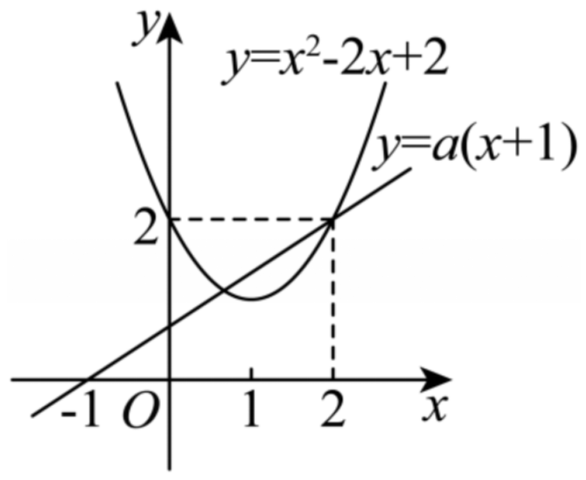
\includegraphics[width=0.30\textwidth]{figures/gao75_q12_graph.png}
\end{center}
% 原卷此处作“≥”，与题干严格不等号方向不一致，照录（见文件头“原卷笔误/存疑”①）
\step{由集合 $A$ 是“$2$ 集合”，故集合 $A$ 中只有一个元素，}
\step{得 $\begin{cases}2^2-2\times2+2\geqslant(2+1)a\\ 1^2-2\times1+2<(1+1)a\end{cases}$，解得 $\dfrac12<a\leqslant\dfrac23$，}
\step{故正实数 $a$ 的取值范围是 $\dfrac12<a\leqslant\dfrac23$.}
\solend
\fi

\end{enumerate}

\bigsec{二、选择题}

\begin{enumerate}
\setcounter{enumi}{12}

\item 已知全集 $U=\R$，集合 $A=\{x\mid x^2<4\}$，$B=\{y\mid y=x^2\}$，则图中阴影部分所表示的集合为\mbox{（\quad）}

\begin{center}
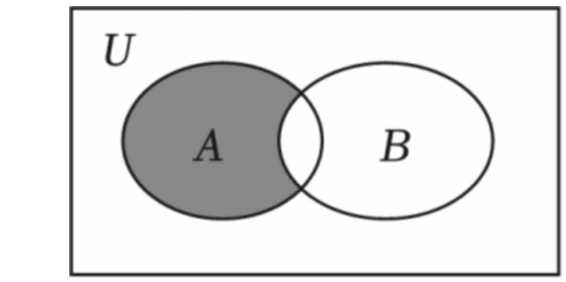
\includegraphics[width=0.26\textwidth]{figures/gao75_q13_venn.png}
\end{center}

\keepwithprev
A. $\{-2,-1,0\}$\qquad B. $(-\infty,4)$\qquad C. $(-2,0)$\qquad D. $(-2,0]$

\ifanswer
\solbegin
\step{集合 $A=\{x\mid x^2<4\}=(-2,2)$，$B=\{y\mid y=x^2\}=[0,+\infty)$，}
\step{图中阴影部分所表示的集合是 $A\cap\overline{B}=(-2,0)$. 故选 $C$.}
\solend
\fi

\item 已知 $x\in\R$，则“$\dfrac1x>1$”是“$x<1$”的\mbox{（\quad）}

\keepwithprev
A. 充分非必要条件\qquad B. 必要非充分条件\qquad C. 充要条件\qquad D. 既非充分又非必要条件

\ifanswer
\solbegin
\step{“$\dfrac1x>1$”$\Leftrightarrow0<x<1$，所以“$\dfrac1x>1$”是“$x<1$”的充分不必要条件. 故选 $A$.}
\solend
\fi

\item 已知集合 $M=\{x\mid x=m+\dfrac16,\,m\in\Z\}$，$N=\{x\mid x=\dfrac n2-\dfrac13,\,n\in\Z\}$，\\
$P=\{x\mid x=\dfrac p2+\dfrac16,\,p\in\Z\}$，则 $M$、$N$、$P$ 的关系为\mbox{（\quad）}

\keepwithprev
A. $M=N\subseteq P$\qquad B. $M\subseteq N=P$\qquad C. $M\subseteq N\subseteq P$\qquad D. $N\subseteq P\subseteq M$

\ifanswer
\solbegin
\step{集合 $N=\{x\mid x=\dfrac n2-\dfrac13,\,n\in\Z\}$，则 $x=\dfrac n2-\dfrac13=\dfrac{3n-2}6$，$n\in\Z$.}
\step{$P=\{x\mid x=\dfrac p2+\dfrac16,\,p\in\Z\}$，则 $x=\dfrac p2+\dfrac16=\dfrac{3p+1}6$，$p\in\Z$.}
\step{$M=\{x\mid x=m+\dfrac16,\,m\in\Z\}$，则 $x=m+\dfrac16=\dfrac{6m+1}6$，$m\in\Z$.}
\step{$M$、$N$、$P$ 三者分母相同，所以只需要比较他们的分子.}
\step{$M$：$6$ 的倍数$+1$，$N=P$：$3$ 的倍数$+1$，所以 $M\subseteq N=P$. 故选 $B$.}
\solend
\fi

\item 设集合 $P_1=\{x\mid x^2+ax+1>0\}$，$P_2=\{x\mid x^2+ax+2>0\}$，$Q_1=\{x\mid x^2+x+b>0\}$，$Q_2=\{x\mid x^2+2x+b>0\}$ 其中 $a,b\in\R$，给出下列两个命题：命题 $q_1$：对任意的 $a$，$P_1$ 是 $P_2$ 的子集；命题 $q_2$：对任意的 $b$，$Q_1$ 不是 $Q_2$ 的子集. 下列说法正确的是\mbox{（\quad）}

\keepwithprev
A. 命题 $q_1$ 是真命题，命题 $q_2$ 是假命题\qquad B. 命题 $q_1$ 是假命题，命题 $q_2$ 是真命题

C. 命题 $q_1$、$q_2$ 都是真命题\qquad D. 命题 $q_1$、$q_2$ 都是假命题

\ifanswer
\solbegin
\step{对于集合 $P_1=\{x\mid x^2+ax+1>0\}$，$P_2=\{x\mid x^2+ax+2>0\}$，}
\step{当 $m\in P_1$，即 $m^2+am+1>0$，得 $m^2+am+2>0$，}
\step{即有 $m\in P_2$，得对任意 $a$，$P_1$ 是 $P_2$ 的子集，命题 $q_1$ 为真命题；}
\step{当 $b=5$ 时，$Q_1=\{x\mid x^2+x+5>0\}=\R$，$Q_2=\{x\mid x^2+2x+5>0\}=\R$，}
\step{得 $Q_1$ 是 $Q_2$ 的子集；}
\step{存在 $b$，使得 $Q_1$ 是 $Q_2$ 的子集，故命题 $q_2$ 是假命题.}
\step{故选 $A$.}
\solend
\fi

\end{enumerate}

\bigsec{三、解答题}

\begin{enumerate}
\setcounter{enumi}{16}

\item 设集合 $A=\{x\mid x^2-2x=0\}$，$B=\{x\mid x^2+2(a+1)x+a^2-1=0\}$.

（1）写出集合 $A$ 的所有子集；

（2）若 $A\cap B=B$，求实数 $a$ 的取值范围.

\ifanswer
\solbegin
\stepm{(1)}{由 $x^2-2x=0$，得 $x=2$ 或 $x=0$，所以 $A=\{0,2\}$，}
\step{故集合 $A$ 的所有子集为 $\varnothing$、$\{0\}$、$\{2\}$、$\{0,2\}$.}
\stepm{(2)}{因为 $A\cap B=B$，所以 $B\subseteq A$，}
\step{方程 $x^2+2(a+1)x+a^2-1=0$，$\Delta=4(a+1)^2-4(a^2-1)=8a+8$，}
\step{若 $\Delta<0$，即 $a<-1$，方程 $x^2+2(a+1)x+a^2-1=0$ 无解，}
\step{此时 $B=\varnothing$，满足题意；}
\step{若 $\Delta=0$，即 $a=-1$，由 $x^2+2(a+1)x+a^2-1=0$，即 $x^2=0$，}
\step{解得 $x=0$，此时 $B=\{0\}$，满足题意；}
\step{若 $\Delta>0$，即 $a>-1$，要使 $B\subseteq A$，}
\step{则方程 $x^2+2(a+1)x+a^2-1=0$ 的解集为 $\{0,2\}$，}
\step{则 $\begin{cases}2+0=-2(a+1)\\ 2\times0=a^2-1\end{cases}$，$a$ 不存在.}
\step{综上所述，$a\leqslant-1$，即实数 $a$ 的取值范围为 $\{a\mid a\leqslant-1\}$.}
\solend
\fi

\ansspace

\item 已知全集 $U=\R$，集合 $A=\left\{x\,\middle|\,\dfrac{x-1}{x-3}<0\right\}$，$B=\{x\mid|x-a|<2\}$.

（1）当 $a=1$ 时，试用区间表示集合 $A$、$B$；

（2）若 $A\cup B=B$，求实数 $a$ 的取值范围.

\ifanswer
\solbegin
\stepm{(1)}{不等式 $\dfrac{x-1}{x-3}<0$ 可化为 $(x-1)(x-3)<0$，解得 $1<x<3$，即 $A=(1,3)$，}
\step{当 $a=1$ 时，$|x-1|<2$，则 $-2<x-1<2$，解得 $-1<x<3$，}
\step{即 $B=(-1,3)$；}
\stepm{(2)}{由不等式 $|x-a|<2$ 得 $-2<x-a<2$，解得 $-2+a<x<2+a$，}
\step{即 $B=\{x\mid-2+a<x<2+a\}$，}
\step{因为 $A\cup B=B$，所以 $A\subseteq B$，则 $\begin{cases}-2+a\leqslant1\\ 2+a\geqslant3\end{cases}$，解得 $1\leqslant a\leqslant3$，}
\step{即实数 $a$ 的取值范围为 $[1,3]$.}
\solend
\fi

\ansspace

\item 法国数学家弗朗索瓦·韦达 1615 年在著作《论方程的识别与订正》中建立了方程根与系数的关系. 发现一元二次方程 $ax^2+bx+c=0$，$a\neq0$ 的根与系数有如下的关系：

$x_1+x_2=-\dfrac ba$，$x_1x_2=\dfrac ca$，此即为韦达定理. 韦达定理的逆定理仍成立：如果两个数 $x_1$，$x_2$ 满足 $x_1+x_2=-\dfrac ba$，$x_1x_2=\dfrac ca$，则这两个数 $x_1$、$x_2$ 是方程 $ax^2+bx+c=0$，$a\neq0$ 的两个根. 例如：$m+n=-3$，$mn=2$，则 $m$、$n$ 是方程 $x^2+3x+2=0$ 的两个根. 请根据上述材料解决以下问题.

（1）已知 $m$、$n$ 是两个不相等的实数，满足 $m^2-6m-5=0$，$n^2-6n-5=0$，求 $\dfrac1m+\dfrac1n$ 的值；

（2）已知实数 $x$、$y$ 满足 $x+y+xy=17$，$x^2y+xy^2=72$，求 $x^2+y^2$ 的值.

\ifanswer
\solbegin
\stepm{(1)}{由题意，不相等的实数 $m$、$n$ 满足 $m^2-6m-5=0$、$n^2-6n-5=0$，}
\step{因此 $m$、$n$ 是一元二次方程 $x^2-6x-5=0$ 的两个不等实根.}
\step{由韦达定理得 $m+n=6$，$mn=-5$，因此 $\dfrac1m+\dfrac1n=\dfrac{m+n}{mn}=\dfrac6{-5}=-\dfrac65$.}
\stepm{(2)}{令 $s=x+y$，$t=xy$，}
\step{因为 $x+y+xy=17$，$x^2y+xy^2=72$，}
\step{即 $x+y+xy=17$，$xy(x+y)=72$，将已知条件变形得 $\begin{cases}s+t=17\\ st=72\end{cases}$.}
\step{由韦达定理逆定理，$s$、$t$ 是一元二次方程 $z^2-17z+72=0$ 的两个实根，}
\step{解方程得 $z_1=8$，$z_2=9$，即有两组解 $\begin{cases}s=8\\ t=9\end{cases}$ 和 $\begin{cases}s=9\\ t=8\end{cases}$.}
\step{当 $\begin{cases}s=8\\ t=9\end{cases}$ 时，$x$、$y$ 是方程 $w^2-8w+9=0$ 的根，}
\step{判别式 $\Delta=8^2-4\times1\times9=64-36=28>0$，符合题意，}
\step{此时 $x^2+y^2=(x+y)^2-2xy=s^2-2t=8^2-2\times9=64-18=46$；}
\step{当 $\begin{cases}s=9\\ t=8\end{cases}$ 时，$x$、$y$ 是方程 $w^2-9w+8=0$ 的根，}
\step{判别式 $\Delta=9^2-4\times1\times8=81-32=49>0$，符合题意，}
\step{此时 $x^2+y^2=(x+y)^2-2xy=s^2-2t=9^2-2\times8=81-16=65$.}
\step{综上，$x^2+y^2$ 的值为 $46$ 或 $65$.}
\solend
\fi

\ansspace

\item 已知关于 $x$ 的不等式 $ax^2-(a+1)x+b<0$.

（1）若不等式的解集是 $\{x\mid1<x<5\}$，求 $a+b$ 的值；

（2）若 $b=-\dfrac12$ 且不等式的解集为 $\R$，求 $a$ 取值范围；

（3）若 $b=1$，讨论此不等式的解集.

\ifanswer
\solbegin
\stepm{(1)}{由题意得 $1$ 和 $5$ 是方程 $ax^2-(a+1)x+b=0$ 的两个根且 $a>0$，}
\step{所以 $1+5=\dfrac{a+1}a$，$1\times5=\dfrac ba$，解得 $a=\dfrac15$，$b=1$，所以 $a+b=\dfrac65$.}
\stepm{(2)}{若 $b=-\dfrac12$，则不等式为 $ax^2-(a+1)x-\dfrac12<0$，}
\step{当 $a\neq0$，则有 $\begin{cases}a<0\\ \Delta=(a+1)^2+2a<0\end{cases}$，解得 $-2-\sqrt3<a<-2+\sqrt3$；}
\step{当 $a=0$，不等式即为 $-x-\dfrac12<0$，则 $x>-\dfrac12$，不合题意；}
\step{所以 $a$ 的取值范围是 $(-2-\sqrt3,-2+\sqrt3)$.}
\stepm{(3)}{若 $b=1$，则不等式为 $ax^2-(a+1)x+1<0$，即 $(ax-1)(x-1)<0$.}
\step{当 $a\neq0$ 时，由 $ax^2-(a+1)x+1<0$ 得 $(ax-1)(x-1)<0$.}
\step{方程 $(ax-1)(x-1)=0$ 的根为 $x=\dfrac1a$ 或 $x=1$，}
\step{当 $0<a<1$ 时，$\dfrac1a>1$，则不等式的解集为 $\left(1,\dfrac1a\right)$；}
\step{当 $a<0$ 时，$\dfrac1a<1$，则不等式的解集为 $\left(-\infty,\dfrac1a\right)\cup(1,+\infty)$；}
\step{当 $a=1$ 时，不等式即为 $(x-1)^2<0$，则不等式的解集为 $\varnothing$；}
\step{当 $a>1$ 时，$\dfrac1a<1$，则不等式的解集为 $\left(\dfrac1a,1\right)$；}
\step{当 $a=0$ 时，不等式为 $-x+1<0$，则不等式的解集为 $(1,+\infty)$；}
\step{综上所述，当 $a<0$ 时，不等式的解集为 $\left(-\infty,\dfrac1a\right)\cup(1,+\infty)$；}
\step{当 $a=0$ 时，不等式的解集为 $(1,+\infty)$；}
\step{当 $0<a<1$ 时，不等式的解集为 $\left(1,\dfrac1a\right)$；}
\step{当 $a=1$ 时，不等式的解集为 $\varnothing$；}
\step{当 $a>1$ 时，不等式的解集为 $\left(\dfrac1a,1\right)$.}
\solend
\fi

\ansspace

\item 已知关于 $x$ 的不等式① $x^2+2cx+c>0$，② $x^2+cx+c^2-1>0$，其中 $c$ 是实数.

（1）若 $1$ 是不等式②的一个解，求实数 $c$ 的取值范围；

（2）证明：不等式①、②中至多有一个恒成立；

（3）当 $c=0$ 时，“$x$ 满足 $|mx^2-4x+3|>5$”的一个必要非充分条件是“$x$ 满足 $x^2+cx+c^2-1>0$，求实数 $m$ 的取值范围.

\ifanswer
\solbegin
\stepm{(1)}{因为 $1$ 是不等式②的一个解，所以 $1+c+c^2-1>0$，}
\step{即 $c(c+1)>0$，解得 $c>0$ 或 $c<-1$，}
\step{所以实数 $c$ 的取值范围为 $(-\infty,-1)\cup(0,+\infty)$.}
\stepm{(2)}{假设不等式①、②都恒成立，}
\step{不等式① $x^2+2cx+c>0$ 恒成立，所以 $4c^2-4c<0$，所以 $0<c<1$；}
\step{② $x^2+cx+c^2-1>0$ 恒成立，所以 $c^2-4(c^2-1)<0$，$c^2>\dfrac43$，}
\step{解得 $c>\dfrac{2\sqrt3}3$ 或 $c<-\dfrac{2\sqrt3}3$；}
\step{所以当不等式①、②都恒成立时，}
\step{不等式组 $\begin{cases}0<c<1\\ c\in\left(-\infty,-\dfrac{2\sqrt3}3\right)\cup\left(\dfrac{2\sqrt3}3,+\infty\right)\end{cases}$ 无解，}
\step{所以假设不成立，}
\step{所以不等式①、②中至多有一个恒成立.}
\stepm{(3)}{当 $c=0$ 时，由 $x^2+cx+c^2-1>0$ 得 $x^2-1>0$，}
\step{解集为 $(-\infty,-1)\cup(1,+\infty)$.}
\step{记集合 $A=\{x\mid|mx^2-4x+3|>5\}$，集合 $B=\{x\mid x<-1\text{ 或 }x>1\}$.}
\step{由“$x$ 满足 $|mx^2-4x+3|>5$”的一个必要非充分条件是}
\step{“$x$ 满足 $x^2+cx+c^2-1>0$”得 $A$ 是 $B$ 的真子集.}
\step{所以 $\overline{B}$ 是 $A$ 的真子集，即对任意 $x\in[-1,1]$，$|mx^2-4x+3|\leqslant5$ 恒成立.}
\step{当 $x=0$ 时，不等式 $-5\leqslant mx^2-4x+3\leqslant5$ 恒成立；}
\step{当 $x\in[-1,0)\cup(0,1]$ 时，}
\step{则 $mx^2-4x+3\geqslant-5$ 与 $mx^2-4x+3\leqslant5$ 同时成立.}
\step{①由 $mx^2-4x+3\geqslant-5$，得 $m\geqslant\dfrac{4x-8}{x^2}$，求值域得 $\dfrac{4x-8}{x^2}$ 的最大值 $=-4$，}
\step{所以 $m\geqslant-4$.}
\step{②由 $mx^2-4x+3\leqslant5$，得 $m\leqslant\dfrac{4x+2}{x^2}$，求值域得 $\dfrac{4x+2}{x^2}$ 的最小值 $=-2$，}
\step{所以 $m\leqslant-2$.}
\step{综上所述，实数 $m$ 的取值范围为 $[-4,-2]$.}
\solend
\fi

\ansspace*[7]

\end{enumerate}

\end{document}
